% **************************************************************************************************************
% A Classic Thesis Style
% An Homage to The Elements of Typographic Style
%
% Copyright (C) 2012 Andr\'e Miede http://www.miede.de
%
% If you like the style then I would appreciate a postcard. My address 
% can be found in the file ClassicThesis.pdf. A collection of the 
% postcards I received so far is available online at 
% http://postcards.miede.de
%
% License:
% This program is free software; you can redistribute it and/or modify
% it under the terms of the GNU General Public License as published by
% the Free Software Foundation; either version 2 of the License, or
% (at your option) any later version.
%
% This program is distributed in the hope that it will be useful,
% but WITHOUT ANY WARRANTY; without even the implied warranty of
% MERCHANTABILITY or FITNESS FOR A PARTICULAR PURPOSE.  See the
% GNU General Public License for more details.
%
% You should have received a copy of the GNU General Public License
% along with this program; see the file COPYING.  If not, write to
% the Free Software Foundation, Inc., 59 Temple Place - Suite 330,
% Boston, MA 02111-1307, USA.
%
% **************************************************************************************************************
% Note:
%    * You must not use "u etc. in strings/commands that will be spaced out (use \"u or real umlauts instead)
%    * New enumeration (small caps): \begin{aenumerate} \end{aenumerate}
%    * For margin notes: \marginpar or \graffito{}
%    * Do not use bold fonts in this style, it is designed around them
%    * Use tables as in the examples
%    * See classicthesis-preamble.sty for useful commands
% **************************************************************************************************************
% To Do:
%		 * [high] Check this out: http://www.golatex.de/koma-script-warnung-in-verbindung-mit-listings-package-t2058.html
%    * [medium] mathbb in section-titles/chapter-titles => disappears somehow in headlines!!!
% **************************************************************************************************************
% Changelog:
%     Modified by Scott Lowe based on changes made by Helen Ramsden for use with University of Edinbugh
%     Ph.D. theses within the School of Informatics.
% **************************************************************************************************************
\documentclass[
	 oneside,openright,titlepage,numbers=noenddot,headinclude,%1headlines,
                footinclude=true,cleardoublepage=empty,
                BCOR=0mm,paper=a4,fontsize=11pt, % Binding correction, paper type and font size
                american, % Languages
                ]{scrreprt}

%********************************************************************
% Note: Make all your adjustments in here
%*******************************************************
% ****************************************************************************************************
% classicthesis-config.tex 
% formerly known as loadpackages.sty, classicthesis-ldpkg.sty, and classicthesis-preamble.sty 
% Use it at the beginning of your ClassicThesis.tex, or as a LaTeX Preamble 
% in your ClassicThesis.{tex,lyx} with % ****************************************************************************************************
% classicthesis-config.tex 
% formerly known as loadpackages.sty, classicthesis-ldpkg.sty, and classicthesis-preamble.sty 
% Use it at the beginning of your ClassicThesis.tex, or as a LaTeX Preamble 
% in your ClassicThesis.{tex,lyx} with % ****************************************************************************************************
% classicthesis-config.tex 
% formerly known as loadpackages.sty, classicthesis-ldpkg.sty, and classicthesis-preamble.sty 
% Use it at the beginning of your ClassicThesis.tex, or as a LaTeX Preamble 
% in your ClassicThesis.{tex,lyx} with \input{classicthesis-config}
% ****************************************************************************************************  
% If you like the classicthesis, then I would appreciate a postcard. 
% My address can be found in the file ClassicThesis.pdf. A collection 
% of the postcards I received so far is available online at 
% http://postcards.miede.de
% ****************************************************************************************************

% ****************************************************************************************************
% 1. Configure classicthesis for your needs here, e.g., remove "drafting" below 
% in order to deactivate the time-stamp on the pages
% ****************************************************************************************************
\PassOptionsToPackage{eulerchapternumbers,listings,%drafting,%
                 pdfspacing,floatperchapter,%linedheaders,%
                 subfig,beramono,parts,%eulermath,
                 dottedtoc}{classicthesis}
% ********************************************************************
% Available options for classicthesis.sty 
% (see ClassicThesis.pdf for more information):
% drafting
% parts nochapters linedheaders
% eulerchapternumbers beramono eulermath pdfspacing minionprospacing
% tocaligned dottedtoc manychapters
% listings floatperchapter subfig
% ********************************************************************

% ********************************************************************
% Triggers for this config
% ******************************************************************** 
\usepackage{ifthen}
\newboolean{enable-backrefs} % enable backrefs in the bibliography
\setboolean{enable-backrefs}{true} % true false
% ****************************************************************************************************


% ****************************************************************************************************
% 2. Personal data and user ad-hoc commands
% ****************************************************************************************************
\newcommand{\myTitle}{Decoding information from neural populations in the visual cortex\xspace}
\newcommand{\mySubtitle}{\xspace}
\newcommand{\myDegree}{Doctor of Philosophy\xspace}
\newcommand{\myName}{Scott C. Lowe\xspace}
\newcommand{\myProf}{Prof. Mark van Rossum,\space\space{University of Edinburgh}\xspace} %Institute for Adaptive and Neural Computation,
\newcommand{\myOtherProf}{Prof. Stefano Panzeri,\space\space{Istituto Italiano di Technologia}\xspace} %Center for Neuroscience and Cognitive Systems,
\newcommand{\myThirdProf}{Prof. Alex Thiele,\space\space{Newcastle University}\xspace} %Institute of Neuroscience,
\newcommand{\mySupervisor}{SUPERVISORNAME\xspace}
\newcommand{\myFaculty}{Institute for Adaptive and Neural Computation\xspace}
\newcommand{\myDepartment}{School of Informatics\xspace}
\newcommand{\myUni}{University of Edinburgh\xspace}
\newcommand{\myLocation}{Edinburgh\xspace}
\newcommand{\myTime}{\the\year\xspace}
\newcommand{\myVersion}{version 4.1\xspace}

% ********************************************************************
% Setup, finetuning, and useful commands
% ********************************************************************
\newcounter{dummy} % necessary for correct hyperlinks (to index, bib, etc.)
\newlength{\abcd} % for ab..z string length calculation
\providecommand{\mLyX}{L\kern-.1667em\lower.25em\hbox{Y}\kern-.125emX\@}
\newcommand{\ie}{i.\,e.}
\newcommand{\Ie}{I.\,e.}
\newcommand{\eg}{e.\,g.}
\newcommand{\Eg}{E.\,g.} 
\newcommand{\etal}{\textit{et al.}}
\newcommand{\NB}{{N.B.}}
% ****************************************************************************************************


% ****************************************************************************************************
% 3. Loading some handy packages
% ****************************************************************************************************
% ******************************************************************** 
% Packages with options that might require adjustments
% ******************************************************************** 
\PassOptionsToPackage{latin9}{inputenc}	% latin9 (ISO-8859-9) = latin1+"Euro sign"
 \usepackage{inputenc}				

%\PassOptionsToPackage{ngerman,american}{babel}   % change this to your language(s)
% Spanish languages need extra options in order to work with this template
%\PassOptionsToPackage{spanish,es-lcroman}{babel}
 \usepackage{babel}					

%\PassOptionsToPackage{square,numbers}{natbib}
 \usepackage[natbibapa]{apacite}
 \usepackage{natbib,natbibspacing}

\PassOptionsToPackage{fleqn}{amsmath}		% math environments and more by the AMS 
 \usepackage{amsmath}

\usepackage{textgreek}

% ******************************************************************** 
% General useful packages
% ******************************************************************** 
\PassOptionsToPackage{T1}{fontenc} % T2A for cyrillics
	\usepackage{fontenc}     
\usepackage{textcomp} % fix warning with missing font shapes
\usepackage{scrhack} % fix warnings when using KOMA with listings package          
\usepackage{xspace} % to get the spacing after macros right  
\usepackage{mparhack} % get marginpar right
\usepackage{fixltx2e} % fixes some LaTeX stuff 
\PassOptionsToPackage{smaller}{acronym} % printonlyused,
	\usepackage{acronym} % nice macros for handling all acronyms in the thesis
%\renewcommand*{\acsfont}[1]{\textssc{#1}} % for MinionPro
%
\ifcsname/bflabel\endcsname%
    % For older versions of acronym
	\renewcommand{\bflabel}[1]{{#1}\hfill} % fix the list of acronyms
\else%
	% For acronym version >=1.41
	% Prevent acronym from using bold face
	\renewcommand{\aclabelfont}[1]{\acsfont{#1}\hfill}
\fi%
%
% ****************************************************************************************************


% ****************************************************************************************************
% 4. Setup floats: tables, (sub)figures, and captions
% ****************************************************************************************************
\usepackage{tabularx} % better tables
	\setlength{\extrarowheight}{3pt} % increase table row height
\newcommand{\tableheadline}[1]{\multicolumn{1}{c}{\spacedlowsmallcaps{#1}}}
\newcommand{\myfloatalign}{\centering} % to be used with each float for alignment
\usepackage{caption}
\DeclareCaptionLabelFormat{spacedlowsmallcaps}{%
  \bothIfFirst{\spacedlowsmallcaps{#1}}{~}\spacedlowsmallcaps{#2}}
\DeclareCaptionLabelSeparator*{periodenspace}{.\enspace}
\captionsetup{%
    hypcap=true,%
    format=plain,%
    indention=0cm,%
    font={small},% ,stretch=1.05
    labelformat=spacedlowsmallcaps,%
    labelsep=periodenspace}
\usepackage{subfig}
\usepackage{rotating}

\usepackage{chngcntr}
% \counterwithin{figure}{section}

% Add padding below caption
% \setlength{\belowcaptionskip}{3pt}

% ****************************************************************************************************
% 4b. Other useful packages
% ****************************************************************************************************
% If you don't have any of these, you can find them on CTAN
%
%\usepackage{bibspacing}     % Don't need to use this, I guess
%
\usepackage{pdflscape}       % Lets you put pages into landscape
\usepackage{rotating}        % Lets you rotate tables and figures
%
\usepackage{keyval}          % Key-value decoder (Part of the graphics bundle, so probably already included)
%
\usepackage{glossaries}      % Comprehensive glossary package
%
% ********************************************************************
% Things for tables
% ********************************************************************
\usepackage{array}           % Extended version of array and table environments
\usepackage{longtable}       % For tables spanning multiple pages
\usepackage{multirow}        % Items can span multiple table rows/cols
\usepackage{dcolumn}                % Lets you align decimal points within columns of a table
\newcolumntype{d}[1]{D{.}{.}{#1}}   % Adds decimal point column type. Must specify the number of decimal places as arg.
% NB: no need to import the (essential) booktabs package, because
% classicthesis.sty does this for us
%
% ********************************************************************
% Laying out text nicely
% ********************************************************************
% Things for maths
\usepackage{amssymb,amstext} % Full math equation support
\usepackage{amsthm}          % Better theorem environments
\usepackage{amsfonts}        % For blackboard bold, etc
\usepackage{nicefrac}        % Nicer fractions
%
%\usepackage{units}           % nice units, for 10Hz with a thin space, etc
\usepackage{siunitx}         % like units, but better
\DeclareSIUnit\cpd{cpd}      % cycles per degree as a cpd unit
\DeclareSIUnit\dva{dva}      % degrees of visual angle unit
\sisetup{separate-uncertainty = true, retain-explicit-plus}
%
\usepackage{mhchem}          % For chemical formulae
%
\usepackage{soul}            % Provides hy­phen­at­able spacing
%
% For displaying text in special ways
\usepackage{verbatim}        % Useful for program listings
% NB: listings (in its own section below) is useful for program listings too.
\usepackage{framed}          % Framed and/or shaded regions
\usepackage{color}           % Set text color
\definecolor{shadecolor}{gray}{0.9} % and make a new named color
%
% ********************************************************************
% Things for including images
% ********************************************************************
\usepackage{grffile}         % allow dots in middle of filenames
\usepackage{epstopdf}        % automatically convert eps files to pdf files
% when using epstopdf, on command line you must call pdflatex with arguments:
%--shell-escape --enable-write18
% NB: we also use the svg package, but that must be done later, after including
% the classicthesis class.
%
% ********************************************************************
% Moving things around
% ********************************************************************
\usepackage{calc}            % Allows raisebox, can move baselines
\usepackage{placeins}        % Provides \FloatBarrier which is an impass for figures 
\usepackage{float}           % Improved float interface
\usepackage{setspace}        % Can set space between lines
%
% ****************************************************************************************************

% ****************************************************************************************************
% 4c. Custom commands
% ****************************************************************************************************
\newcommand{\lyxdot}{.}
\newcommand{\mm}[0]{$\mathrm{\mu m}$ }
%\newcommand{\degree}{\ensuremath{^\circ}}
\newcommand{\ih}[0]{$I_{h}$ }
\newcommand{\cm}[0]{$cm^{2}$}
\newcommand{\sq}[0]{$^{2}$ }
% ********************************************************************
% Maths things
% ********************************************************************
% Declare a font which is useful for making symbols as curly letters,
% such as \mathpzc{H}
\DeclareMathAlphabet{\mathpzc}{OT1}{pzc}{m}{it}
%%% `Log-like' maths functions
\DeclareMathOperator{\sgn}{sgn}                         % sign
\DeclareMathOperator{\E}{\mathop{\mathbb E\/}}         % expectation
\DeclareMathOperator*{\EE}{\mathlarger{\mathlarger{\mathop{\mathbb E\/}}}}   % expectation
%\newcommand{\EE}{\mathlarger{\operatorname{\mathbb E}}}
\DeclareMathOperator{\PP}{\mathbb P\/}  % probability
%
% Derivatives
\let\underdot=\d                                        % rename builtin command \d{} to \underdot{}
%\renewcommand{\d}{\operatorname{d}}                     % old method
\renewcommand{\d}{\ensuremath{\operatorname{d}\!}}      % straight operator d (\! for no space after)
%\renewcommand{\d}{\ensuremath{d}}                       % italic (variable-like) d
\newcommand{\od}[1]{\frac{\d}{\d#1}}                    % first order ordinary derivative operator
\newcommand{\odn}[2]{\frac{\d^{#2}}{\d#1^{#2}}}         % n-th order ordinary derivative operator
\newcommand{\pd}[1]{\frac{\partial}{\partial #1}}       % first order partial derivative operator
\newcommand{\pdn}[2]{\frac{\partial^{#2}}{\partial #1^{#2}}}    % n-th order partial derivative operator
%
%%% Ordinals
%\newcommand{\ord}[2]{#1#2}                              %where we are doing normal 1st, 2nd, 3rd, 4th and not n-th
\newcommand{\ord}[2]{\ensuremath{\text{#1}^\text{#2}}}  %where we are doing normal 1st, 2nd, 3rd, 4th and not n-th
%\newcommand{\nth}[1]{#1\text{-th}}                      %where the argument is mathematical and we are in math-mode
%\newcommand{\mth}[1]{$#1$-th}                           %where the argument is mathematical but we are not in math-mode
\newcommand{\nth}[1]{\ensuremath{#1\text{-th}}}         %NEW: where argument is mathematical (may be used in any mode)
\newcommand{\mth}[1]{\nth{#1}}                          %ditto. for backward compatibility.
%
%%% Vectors
\newcommand{\mtx}[1]{\left[ \begin{matrix} #1 \end{matrix} \right]} %matrix
\newcommand{\col}[1]{\mtx{#1}}                                      %column vector
\newcommand{\row}[1]{[#1]}                                          %row vector
\newcommand{\tcol}[1]{\row{#1}^T}                                   %transposed col vector
%
%%% Notation
\newcommand{\VEC}[1]{\mathbf{#1}}                                   %vector symbol typeface
\newcommand{\SET}[1]{\mathbf{#1}}                                   %set symbol typeface
\newcommand{\NSYS}[1]{\mathbb{#1}}                                  %number system typeface (R, C, Z, N)
%
\newcommand{\R}{\NSYS{R}}                                           %number system typeface (R, C, Z, N)
\newcommand{\C}{\NSYS{C}}                                           %number system typeface (R, C, Z, N)
\newcommand{\Z}{\NSYS{Z}}                                           %number system typeface (R, C, Z, N)
\newcommand{\N}{\NSYS{N}}                                           %number system typeface (R, C, Z, N)
%
%% Imaginary unit
\newcommand{\iu}{{\mathrm{i}\mkern1mu}}
%% Real and Imaginary components
\renewcommand{\Re}{\operatorname{Re}}
\renewcommand{\Im}{\operatorname{Im}}
%
% ****************************************************************************************************

% ****************************************************************************************************
% 5. Setup code listings
% ****************************************************************************************************
\usepackage{listings} 
%\lstset{emph={trueIndex,root},emphstyle=\color{BlueViolet}}%\underbar} % for special keywords
\lstset{language=[LaTeX]Tex,%C++,
    keywordstyle=\color{RoyalBlue},%\bfseries,
    basicstyle=\small\ttfamily,
    %identifierstyle=\color{NavyBlue},
    commentstyle=\color{Green}\ttfamily,
    stringstyle=\rmfamily,
    numbers=none,%left,%
    numberstyle=\scriptsize,%\tiny
    stepnumber=5,
    numbersep=8pt,
    showstringspaces=false,
    breaklines=true,
    frameround=ftff,
    frame=single,
    belowcaptionskip=.75\baselineskip
    %frame=L
} 
% ****************************************************************************************************    		   


% ****************************************************************************************************
% 6. PDFLaTeX, hyperreferences and citation backreferences
% ****************************************************************************************************
% ********************************************************************
% Using PDFLaTeX
% ********************************************************************
\PassOptionsToPackage{pdftex,hyperfootnotes=false,pdfpagelabels,backref=page}{hyperref}
	\usepackage{hyperref}  % backref linktocpage pagebackref

\pdfcompresslevel=9
\pdfadjustspacing=1 
\PassOptionsToPackage{pdftex}{graphicx}
	\usepackage{graphicx} 

% ********************************************************************
% Setup the style of the backrefs from the bibliography
% (translate the options to any language you use)
% ********************************************************************
\newcommand{\backrefnotcitedstring}{\relax}%(Not cited.)
\newcommand{\backrefcitedsinglestring}[1]{(Cited on page~#1.)}
\newcommand{\backrefcitedmultistring}[1]{(Cited on pages~#1.)}
\ifthenelse{\boolean{enable-backrefs}}%
{%
		\PassOptionsToPackage{hyperpageref}{backref}
		\usepackage{backref} % to be loaded after hyperref package 
		   \renewcommand{\backreftwosep}{ and~} % separate 2 pages
		   \renewcommand{\backreflastsep}{, and~} % separate last of longer list
		   \renewcommand*{\backref}[1]{}  % disable standard
		   \renewcommand*{\backrefalt}[4]{% detailed backref
		      \ifcase #1 %
		         \backrefnotcitedstring%
		      \or%
		         \backrefcitedsinglestring{#2}%
		      \else%
		         \backrefcitedmultistring{#2}%
		      \fi}%
}{\relax}    

% ********************************************************************
% Hyperreferences
% ********************************************************************
\definecolor{webblue}{rgb}{0,0,0.930}
\hypersetup{%
    %draft,	% = no hyperlinking at all (useful in b/w printouts)
    colorlinks=true, linktocpage=true, pdfstartpage=3, pdfstartview=FitV,%
    % uncomment the following line if you want to have black links (e.g., for printing)
    %colorlinks=false, linktocpage=false, pdfborder={0 0 0}, pdfstartpage=3, pdfstartview=FitV,% 
    breaklinks=true, pdfpagemode=UseNone, pageanchor=true, pdfpagemode=UseOutlines,%
    plainpages=false, bookmarksnumbered, bookmarksopen=true, bookmarksopenlevel=1,%
    hypertexnames=true, pdfhighlight=/O,%nesting=true,%frenchlinks,%
    urlcolor=webbrown, linkcolor=RoyalBlue, citecolor=webgreen, %pagecolor=RoyalBlue,%
    %urlcolor=Black, linkcolor=Black, citecolor=Black, %pagecolor=Black,%
    pdftitle={\myTitle},%
    pdfauthor={\textcopyright\ \myName, \myUni, \myFaculty},%
    pdfsubject={},%
    pdfkeywords={},%
    pdfcreator={pdfLaTeX},%
    pdfproducer={LaTeX with hyperref and classicthesis}%
}   

% ********************************************************************
% Setup autoreferences
% ********************************************************************
% There are some issues regarding autorefnames
% http://www.ureader.de/msg/136221647.aspx
% http://www.tex.ac.uk/cgi-bin/texfaq2html?label=latexwords
% you have to redefine the makros for the 
% language you use, e.g., american, ngerman
% (as chosen when loading babel/AtBeginDocument)
% ********************************************************************
\makeatletter
\@ifpackageloaded{babel}%
    {%
       \addto\extrasamerican{%
					\renewcommand*{\figureautorefname}{Figure}%
					\renewcommand*{\tableautorefname}{Table}%
					\renewcommand*{\partautorefname}{Part}%
					\renewcommand*{\chapterautorefname}{Chapter}%
					\renewcommand*{\sectionautorefname}{Section}%
					\renewcommand*{\subsectionautorefname}{Section}%
					\renewcommand*{\subsubsectionautorefname}{Section}% 	
				}%
       \addto\extrasngerman{% 
					\renewcommand*{\paragraphautorefname}{Absatz}%
					\renewcommand*{\subparagraphautorefname}{Unterabsatz}%
					\renewcommand*{\footnoteautorefname}{Fu\"snote}%
					\renewcommand*{\FancyVerbLineautorefname}{Zeile}%
					\renewcommand*{\theoremautorefname}{Theorem}%
					\renewcommand*{\appendixautorefname}{Anhang}%
					\renewcommand*{\equationautorefname}{Gleichung}%        
					\renewcommand*{\itemautorefname}{Punkt}%
				}%	
			% Fix to getting autorefs for subfigures right (thanks to Belinda Vogt for changing the definition)
			\providecommand{\subfigureautorefname}{\figureautorefname}%  			
    }{\relax}
\makeatother


% ****************************************************************************************************
% 7. Last calls before the bar closes
% ****************************************************************************************************
% ********************************************************************
% Development Stuff
% ********************************************************************
\listfiles
%\PassOptionsToPackage{l2tabu,orthodox,abort}{nag}
%	\usepackage{nag}
%\PassOptionsToPackage{warning, all}{onlyamsmath}
%	\usepackage{onlyamsmath}

% ********************************************************************
% Last, but not least...
% ********************************************************************
\usepackage{classicthesis} 
% ****************************************************************************************************

% ****************************************************************************************************
% 8. Further adjustments (experimental)
% ****************************************************************************************************
% ********************************************************************
% Import svg package
% ********************************************************************
% Need to include the svg package after classicthesis because it does not
% play nicely with importing several required packages too early
\usepackage{svg}             % can include svg files with \includesvg

% ********************************************************************
% Changing the text area
% ********************************************************************
% \linespread{1.3}
\linespread{1.05} % a bit more for Palatino
%\areaset[current]{312pt}{761pt} % 686 (factor 2.2) + 33 head + 42 head \the\footskip
%\setlength{\marginparwidth}{7em}%
%\setlength{\marginparsep}{2em}%

% ********************************************************************
% Using different fonts
% ********************************************************************
%\usepackage[oldstylenums]{kpfonts} % oldstyle notextcomp
%\usepackage[osf]{libertine}
%\usepackage{hfoldsty} % Computer Modern with osf
%\usepackage[light,condensed,math]{iwona}
%\renewcommand{\sfdefault}{iwona}
%\usepackage{lmodern} % <-- no osf support :-(
%\usepackage[urw-garamond]{mathdesign} <-- no osf support :-(

% ********************************************************************
% Adjust colour of acronyms
% ********************************************************************
\makeatletter
\AtBeginDocument{%
  \renewcommand*{\AC@hyperlink}[2]{%
    \begingroup
      \hypersetup{linkcolor=Black}%webbrown
      \hyperlink{#1}{#2}%
    \endgroup
  }%
}
\makeatother
% ****************************************************************************************************

% ****************************************************************************************************  
% If you like the classicthesis, then I would appreciate a postcard. 
% My address can be found in the file ClassicThesis.pdf. A collection 
% of the postcards I received so far is available online at 
% http://postcards.miede.de
% ****************************************************************************************************

% ****************************************************************************************************
% 1. Configure classicthesis for your needs here, e.g., remove "drafting" below 
% in order to deactivate the time-stamp on the pages
% ****************************************************************************************************
\PassOptionsToPackage{eulerchapternumbers,listings,%drafting,%
                 pdfspacing,floatperchapter,%linedheaders,%
                 subfig,beramono,parts,%eulermath,
                 dottedtoc}{classicthesis}
% ********************************************************************
% Available options for classicthesis.sty 
% (see ClassicThesis.pdf for more information):
% drafting
% parts nochapters linedheaders
% eulerchapternumbers beramono eulermath pdfspacing minionprospacing
% tocaligned dottedtoc manychapters
% listings floatperchapter subfig
% ********************************************************************

% ********************************************************************
% Triggers for this config
% ******************************************************************** 
\usepackage{ifthen}
\newboolean{enable-backrefs} % enable backrefs in the bibliography
\setboolean{enable-backrefs}{true} % true false
% ****************************************************************************************************


% ****************************************************************************************************
% 2. Personal data and user ad-hoc commands
% ****************************************************************************************************
\newcommand{\myTitle}{Decoding information from neural populations in the visual cortex\xspace}
\newcommand{\mySubtitle}{\xspace}
\newcommand{\myDegree}{Doctor of Philosophy\xspace}
\newcommand{\myName}{Scott C. Lowe\xspace}
\newcommand{\myProf}{Prof. Mark van Rossum,\space\space{University of Edinburgh}\xspace} %Institute for Adaptive and Neural Computation,
\newcommand{\myOtherProf}{Prof. Stefano Panzeri,\space\space{Istituto Italiano di Technologia}\xspace} %Center for Neuroscience and Cognitive Systems,
\newcommand{\myThirdProf}{Prof. Alex Thiele,\space\space{Newcastle University}\xspace} %Institute of Neuroscience,
\newcommand{\mySupervisor}{SUPERVISORNAME\xspace}
\newcommand{\myFaculty}{Institute for Adaptive and Neural Computation\xspace}
\newcommand{\myDepartment}{School of Informatics\xspace}
\newcommand{\myUni}{University of Edinburgh\xspace}
\newcommand{\myLocation}{Edinburgh\xspace}
\newcommand{\myTime}{\the\year\xspace}
\newcommand{\myVersion}{version 4.1\xspace}

% ********************************************************************
% Setup, finetuning, and useful commands
% ********************************************************************
\newcounter{dummy} % necessary for correct hyperlinks (to index, bib, etc.)
\newlength{\abcd} % for ab..z string length calculation
\providecommand{\mLyX}{L\kern-.1667em\lower.25em\hbox{Y}\kern-.125emX\@}
\newcommand{\ie}{i.\,e.}
\newcommand{\Ie}{I.\,e.}
\newcommand{\eg}{e.\,g.}
\newcommand{\Eg}{E.\,g.} 
\newcommand{\etal}{\textit{et al.}}
\newcommand{\NB}{{N.B.}}
% ****************************************************************************************************


% ****************************************************************************************************
% 3. Loading some handy packages
% ****************************************************************************************************
% ******************************************************************** 
% Packages with options that might require adjustments
% ******************************************************************** 
\PassOptionsToPackage{latin9}{inputenc}	% latin9 (ISO-8859-9) = latin1+"Euro sign"
 \usepackage{inputenc}				

%\PassOptionsToPackage{ngerman,american}{babel}   % change this to your language(s)
% Spanish languages need extra options in order to work with this template
%\PassOptionsToPackage{spanish,es-lcroman}{babel}
 \usepackage{babel}					

%\PassOptionsToPackage{square,numbers}{natbib}
 \usepackage[natbibapa]{apacite}
 \usepackage{natbib,natbibspacing}

\PassOptionsToPackage{fleqn}{amsmath}		% math environments and more by the AMS 
 \usepackage{amsmath}

\usepackage{textgreek}

% ******************************************************************** 
% General useful packages
% ******************************************************************** 
\PassOptionsToPackage{T1}{fontenc} % T2A for cyrillics
	\usepackage{fontenc}     
\usepackage{textcomp} % fix warning with missing font shapes
\usepackage{scrhack} % fix warnings when using KOMA with listings package          
\usepackage{xspace} % to get the spacing after macros right  
\usepackage{mparhack} % get marginpar right
\usepackage{fixltx2e} % fixes some LaTeX stuff 
\PassOptionsToPackage{smaller}{acronym} % printonlyused,
	\usepackage{acronym} % nice macros for handling all acronyms in the thesis
%\renewcommand*{\acsfont}[1]{\textssc{#1}} % for MinionPro
%
\ifcsname/bflabel\endcsname%
    % For older versions of acronym
	\renewcommand{\bflabel}[1]{{#1}\hfill} % fix the list of acronyms
\else%
	% For acronym version >=1.41
	% Prevent acronym from using bold face
	\renewcommand{\aclabelfont}[1]{\acsfont{#1}\hfill}
\fi%
%
% ****************************************************************************************************


% ****************************************************************************************************
% 4. Setup floats: tables, (sub)figures, and captions
% ****************************************************************************************************
\usepackage{tabularx} % better tables
	\setlength{\extrarowheight}{3pt} % increase table row height
\newcommand{\tableheadline}[1]{\multicolumn{1}{c}{\spacedlowsmallcaps{#1}}}
\newcommand{\myfloatalign}{\centering} % to be used with each float for alignment
\usepackage{caption}
\DeclareCaptionLabelFormat{spacedlowsmallcaps}{%
  \bothIfFirst{\spacedlowsmallcaps{#1}}{~}\spacedlowsmallcaps{#2}}
\DeclareCaptionLabelSeparator*{periodenspace}{.\enspace}
\captionsetup{%
    hypcap=true,%
    format=plain,%
    indention=0cm,%
    font={small},% ,stretch=1.05
    labelformat=spacedlowsmallcaps,%
    labelsep=periodenspace}
\usepackage{subfig}
\usepackage{rotating}

\usepackage{chngcntr}
% \counterwithin{figure}{section}

% Add padding below caption
% \setlength{\belowcaptionskip}{3pt}

% ****************************************************************************************************
% 4b. Other useful packages
% ****************************************************************************************************
% If you don't have any of these, you can find them on CTAN
%
%\usepackage{bibspacing}     % Don't need to use this, I guess
%
\usepackage{pdflscape}       % Lets you put pages into landscape
\usepackage{rotating}        % Lets you rotate tables and figures
%
\usepackage{keyval}          % Key-value decoder (Part of the graphics bundle, so probably already included)
%
\usepackage{glossaries}      % Comprehensive glossary package
%
% ********************************************************************
% Things for tables
% ********************************************************************
\usepackage{array}           % Extended version of array and table environments
\usepackage{longtable}       % For tables spanning multiple pages
\usepackage{multirow}        % Items can span multiple table rows/cols
\usepackage{dcolumn}                % Lets you align decimal points within columns of a table
\newcolumntype{d}[1]{D{.}{.}{#1}}   % Adds decimal point column type. Must specify the number of decimal places as arg.
% NB: no need to import the (essential) booktabs package, because
% classicthesis.sty does this for us
%
% ********************************************************************
% Laying out text nicely
% ********************************************************************
% Things for maths
\usepackage{amssymb,amstext} % Full math equation support
\usepackage{amsthm}          % Better theorem environments
\usepackage{amsfonts}        % For blackboard bold, etc
\usepackage{nicefrac}        % Nicer fractions
%
%\usepackage{units}           % nice units, for 10Hz with a thin space, etc
\usepackage{siunitx}         % like units, but better
\DeclareSIUnit\cpd{cpd}      % cycles per degree as a cpd unit
\DeclareSIUnit\dva{dva}      % degrees of visual angle unit
\sisetup{separate-uncertainty = true, retain-explicit-plus}
%
\usepackage{mhchem}          % For chemical formulae
%
\usepackage{soul}            % Provides hy­phen­at­able spacing
%
% For displaying text in special ways
\usepackage{verbatim}        % Useful for program listings
% NB: listings (in its own section below) is useful for program listings too.
\usepackage{framed}          % Framed and/or shaded regions
\usepackage{color}           % Set text color
\definecolor{shadecolor}{gray}{0.9} % and make a new named color
%
% ********************************************************************
% Things for including images
% ********************************************************************
\usepackage{grffile}         % allow dots in middle of filenames
\usepackage{epstopdf}        % automatically convert eps files to pdf files
% when using epstopdf, on command line you must call pdflatex with arguments:
%--shell-escape --enable-write18
% NB: we also use the svg package, but that must be done later, after including
% the classicthesis class.
%
% ********************************************************************
% Moving things around
% ********************************************************************
\usepackage{calc}            % Allows raisebox, can move baselines
\usepackage{placeins}        % Provides \FloatBarrier which is an impass for figures 
\usepackage{float}           % Improved float interface
\usepackage{setspace}        % Can set space between lines
%
% ****************************************************************************************************

% ****************************************************************************************************
% 4c. Custom commands
% ****************************************************************************************************
\newcommand{\lyxdot}{.}
\newcommand{\mm}[0]{$\mathrm{\mu m}$ }
%\newcommand{\degree}{\ensuremath{^\circ}}
\newcommand{\ih}[0]{$I_{h}$ }
\newcommand{\cm}[0]{$cm^{2}$}
\newcommand{\sq}[0]{$^{2}$ }
% ********************************************************************
% Maths things
% ********************************************************************
% Declare a font which is useful for making symbols as curly letters,
% such as \mathpzc{H}
\DeclareMathAlphabet{\mathpzc}{OT1}{pzc}{m}{it}
%%% `Log-like' maths functions
\DeclareMathOperator{\sgn}{sgn}                         % sign
\DeclareMathOperator{\E}{\mathop{\mathbb E\/}}         % expectation
\DeclareMathOperator*{\EE}{\mathlarger{\mathlarger{\mathop{\mathbb E\/}}}}   % expectation
%\newcommand{\EE}{\mathlarger{\operatorname{\mathbb E}}}
\DeclareMathOperator{\PP}{\mathbb P\/}  % probability
%
% Derivatives
\let\underdot=\d                                        % rename builtin command \d{} to \underdot{}
%\renewcommand{\d}{\operatorname{d}}                     % old method
\renewcommand{\d}{\ensuremath{\operatorname{d}\!}}      % straight operator d (\! for no space after)
%\renewcommand{\d}{\ensuremath{d}}                       % italic (variable-like) d
\newcommand{\od}[1]{\frac{\d}{\d#1}}                    % first order ordinary derivative operator
\newcommand{\odn}[2]{\frac{\d^{#2}}{\d#1^{#2}}}         % n-th order ordinary derivative operator
\newcommand{\pd}[1]{\frac{\partial}{\partial #1}}       % first order partial derivative operator
\newcommand{\pdn}[2]{\frac{\partial^{#2}}{\partial #1^{#2}}}    % n-th order partial derivative operator
%
%%% Ordinals
%\newcommand{\ord}[2]{#1#2}                              %where we are doing normal 1st, 2nd, 3rd, 4th and not n-th
\newcommand{\ord}[2]{\ensuremath{\text{#1}^\text{#2}}}  %where we are doing normal 1st, 2nd, 3rd, 4th and not n-th
%\newcommand{\nth}[1]{#1\text{-th}}                      %where the argument is mathematical and we are in math-mode
%\newcommand{\mth}[1]{$#1$-th}                           %where the argument is mathematical but we are not in math-mode
\newcommand{\nth}[1]{\ensuremath{#1\text{-th}}}         %NEW: where argument is mathematical (may be used in any mode)
\newcommand{\mth}[1]{\nth{#1}}                          %ditto. for backward compatibility.
%
%%% Vectors
\newcommand{\mtx}[1]{\left[ \begin{matrix} #1 \end{matrix} \right]} %matrix
\newcommand{\col}[1]{\mtx{#1}}                                      %column vector
\newcommand{\row}[1]{[#1]}                                          %row vector
\newcommand{\tcol}[1]{\row{#1}^T}                                   %transposed col vector
%
%%% Notation
\newcommand{\VEC}[1]{\mathbf{#1}}                                   %vector symbol typeface
\newcommand{\SET}[1]{\mathbf{#1}}                                   %set symbol typeface
\newcommand{\NSYS}[1]{\mathbb{#1}}                                  %number system typeface (R, C, Z, N)
%
\newcommand{\R}{\NSYS{R}}                                           %number system typeface (R, C, Z, N)
\newcommand{\C}{\NSYS{C}}                                           %number system typeface (R, C, Z, N)
\newcommand{\Z}{\NSYS{Z}}                                           %number system typeface (R, C, Z, N)
\newcommand{\N}{\NSYS{N}}                                           %number system typeface (R, C, Z, N)
%
%% Imaginary unit
\newcommand{\iu}{{\mathrm{i}\mkern1mu}}
%% Real and Imaginary components
\renewcommand{\Re}{\operatorname{Re}}
\renewcommand{\Im}{\operatorname{Im}}
%
% ****************************************************************************************************

% ****************************************************************************************************
% 5. Setup code listings
% ****************************************************************************************************
\usepackage{listings} 
%\lstset{emph={trueIndex,root},emphstyle=\color{BlueViolet}}%\underbar} % for special keywords
\lstset{language=[LaTeX]Tex,%C++,
    keywordstyle=\color{RoyalBlue},%\bfseries,
    basicstyle=\small\ttfamily,
    %identifierstyle=\color{NavyBlue},
    commentstyle=\color{Green}\ttfamily,
    stringstyle=\rmfamily,
    numbers=none,%left,%
    numberstyle=\scriptsize,%\tiny
    stepnumber=5,
    numbersep=8pt,
    showstringspaces=false,
    breaklines=true,
    frameround=ftff,
    frame=single,
    belowcaptionskip=.75\baselineskip
    %frame=L
} 
% ****************************************************************************************************    		   


% ****************************************************************************************************
% 6. PDFLaTeX, hyperreferences and citation backreferences
% ****************************************************************************************************
% ********************************************************************
% Using PDFLaTeX
% ********************************************************************
\PassOptionsToPackage{pdftex,hyperfootnotes=false,pdfpagelabels,backref=page}{hyperref}
	\usepackage{hyperref}  % backref linktocpage pagebackref

\pdfcompresslevel=9
\pdfadjustspacing=1 
\PassOptionsToPackage{pdftex}{graphicx}
	\usepackage{graphicx} 

% ********************************************************************
% Setup the style of the backrefs from the bibliography
% (translate the options to any language you use)
% ********************************************************************
\newcommand{\backrefnotcitedstring}{\relax}%(Not cited.)
\newcommand{\backrefcitedsinglestring}[1]{(Cited on page~#1.)}
\newcommand{\backrefcitedmultistring}[1]{(Cited on pages~#1.)}
\ifthenelse{\boolean{enable-backrefs}}%
{%
		\PassOptionsToPackage{hyperpageref}{backref}
		\usepackage{backref} % to be loaded after hyperref package 
		   \renewcommand{\backreftwosep}{ and~} % separate 2 pages
		   \renewcommand{\backreflastsep}{, and~} % separate last of longer list
		   \renewcommand*{\backref}[1]{}  % disable standard
		   \renewcommand*{\backrefalt}[4]{% detailed backref
		      \ifcase #1 %
		         \backrefnotcitedstring%
		      \or%
		         \backrefcitedsinglestring{#2}%
		      \else%
		         \backrefcitedmultistring{#2}%
		      \fi}%
}{\relax}    

% ********************************************************************
% Hyperreferences
% ********************************************************************
\definecolor{webblue}{rgb}{0,0,0.930}
\hypersetup{%
    %draft,	% = no hyperlinking at all (useful in b/w printouts)
    colorlinks=true, linktocpage=true, pdfstartpage=3, pdfstartview=FitV,%
    % uncomment the following line if you want to have black links (e.g., for printing)
    %colorlinks=false, linktocpage=false, pdfborder={0 0 0}, pdfstartpage=3, pdfstartview=FitV,% 
    breaklinks=true, pdfpagemode=UseNone, pageanchor=true, pdfpagemode=UseOutlines,%
    plainpages=false, bookmarksnumbered, bookmarksopen=true, bookmarksopenlevel=1,%
    hypertexnames=true, pdfhighlight=/O,%nesting=true,%frenchlinks,%
    urlcolor=webbrown, linkcolor=RoyalBlue, citecolor=webgreen, %pagecolor=RoyalBlue,%
    %urlcolor=Black, linkcolor=Black, citecolor=Black, %pagecolor=Black,%
    pdftitle={\myTitle},%
    pdfauthor={\textcopyright\ \myName, \myUni, \myFaculty},%
    pdfsubject={},%
    pdfkeywords={},%
    pdfcreator={pdfLaTeX},%
    pdfproducer={LaTeX with hyperref and classicthesis}%
}   

% ********************************************************************
% Setup autoreferences
% ********************************************************************
% There are some issues regarding autorefnames
% http://www.ureader.de/msg/136221647.aspx
% http://www.tex.ac.uk/cgi-bin/texfaq2html?label=latexwords
% you have to redefine the makros for the 
% language you use, e.g., american, ngerman
% (as chosen when loading babel/AtBeginDocument)
% ********************************************************************
\makeatletter
\@ifpackageloaded{babel}%
    {%
       \addto\extrasamerican{%
					\renewcommand*{\figureautorefname}{Figure}%
					\renewcommand*{\tableautorefname}{Table}%
					\renewcommand*{\partautorefname}{Part}%
					\renewcommand*{\chapterautorefname}{Chapter}%
					\renewcommand*{\sectionautorefname}{Section}%
					\renewcommand*{\subsectionautorefname}{Section}%
					\renewcommand*{\subsubsectionautorefname}{Section}% 	
				}%
       \addto\extrasngerman{% 
					\renewcommand*{\paragraphautorefname}{Absatz}%
					\renewcommand*{\subparagraphautorefname}{Unterabsatz}%
					\renewcommand*{\footnoteautorefname}{Fu\"snote}%
					\renewcommand*{\FancyVerbLineautorefname}{Zeile}%
					\renewcommand*{\theoremautorefname}{Theorem}%
					\renewcommand*{\appendixautorefname}{Anhang}%
					\renewcommand*{\equationautorefname}{Gleichung}%        
					\renewcommand*{\itemautorefname}{Punkt}%
				}%	
			% Fix to getting autorefs for subfigures right (thanks to Belinda Vogt for changing the definition)
			\providecommand{\subfigureautorefname}{\figureautorefname}%  			
    }{\relax}
\makeatother


% ****************************************************************************************************
% 7. Last calls before the bar closes
% ****************************************************************************************************
% ********************************************************************
% Development Stuff
% ********************************************************************
\listfiles
%\PassOptionsToPackage{l2tabu,orthodox,abort}{nag}
%	\usepackage{nag}
%\PassOptionsToPackage{warning, all}{onlyamsmath}
%	\usepackage{onlyamsmath}

% ********************************************************************
% Last, but not least...
% ********************************************************************
\usepackage{classicthesis} 
% ****************************************************************************************************

% ****************************************************************************************************
% 8. Further adjustments (experimental)
% ****************************************************************************************************
% ********************************************************************
% Import svg package
% ********************************************************************
% Need to include the svg package after classicthesis because it does not
% play nicely with importing several required packages too early
\usepackage{svg}             % can include svg files with \includesvg

% ********************************************************************
% Changing the text area
% ********************************************************************
% \linespread{1.3}
\linespread{1.05} % a bit more for Palatino
%\areaset[current]{312pt}{761pt} % 686 (factor 2.2) + 33 head + 42 head \the\footskip
%\setlength{\marginparwidth}{7em}%
%\setlength{\marginparsep}{2em}%

% ********************************************************************
% Using different fonts
% ********************************************************************
%\usepackage[oldstylenums]{kpfonts} % oldstyle notextcomp
%\usepackage[osf]{libertine}
%\usepackage{hfoldsty} % Computer Modern with osf
%\usepackage[light,condensed,math]{iwona}
%\renewcommand{\sfdefault}{iwona}
%\usepackage{lmodern} % <-- no osf support :-(
%\usepackage[urw-garamond]{mathdesign} <-- no osf support :-(

% ********************************************************************
% Adjust colour of acronyms
% ********************************************************************
\makeatletter
\AtBeginDocument{%
  \renewcommand*{\AC@hyperlink}[2]{%
    \begingroup
      \hypersetup{linkcolor=Black}%webbrown
      \hyperlink{#1}{#2}%
    \endgroup
  }%
}
\makeatother
% ****************************************************************************************************

% ****************************************************************************************************  
% If you like the classicthesis, then I would appreciate a postcard. 
% My address can be found in the file ClassicThesis.pdf. A collection 
% of the postcards I received so far is available online at 
% http://postcards.miede.de
% ****************************************************************************************************

% ****************************************************************************************************
% 1. Configure classicthesis for your needs here, e.g., remove "drafting" below 
% in order to deactivate the time-stamp on the pages
% ****************************************************************************************************
\PassOptionsToPackage{eulerchapternumbers,listings,%drafting,%
                 pdfspacing,floatperchapter,%linedheaders,%
                 subfig,beramono,parts,%eulermath,
                 dottedtoc}{classicthesis}
% ********************************************************************
% Available options for classicthesis.sty 
% (see ClassicThesis.pdf for more information):
% drafting
% parts nochapters linedheaders
% eulerchapternumbers beramono eulermath pdfspacing minionprospacing
% tocaligned dottedtoc manychapters
% listings floatperchapter subfig
% ********************************************************************

% ********************************************************************
% Triggers for this config
% ******************************************************************** 
\usepackage{ifthen}
\newboolean{enable-backrefs} % enable backrefs in the bibliography
\setboolean{enable-backrefs}{true} % true false
% ****************************************************************************************************


% ****************************************************************************************************
% 2. Personal data and user ad-hoc commands
% ****************************************************************************************************
\newcommand{\myTitle}{Decoding information from neural populations in the visual cortex\xspace}
\newcommand{\mySubtitle}{\xspace}
\newcommand{\myDegree}{Doctor of Philosophy\xspace}
\newcommand{\myName}{Scott C. Lowe\xspace}
\newcommand{\myProf}{Prof. Mark van Rossum,\space\space{University of Edinburgh}\xspace} %Institute for Adaptive and Neural Computation,
\newcommand{\myOtherProf}{Prof. Stefano Panzeri,\space\space{Istituto Italiano di Technologia}\xspace} %Center for Neuroscience and Cognitive Systems,
\newcommand{\myThirdProf}{Prof. Alex Thiele,\space\space{Newcastle University}\xspace} %Institute of Neuroscience,
\newcommand{\mySupervisor}{SUPERVISORNAME\xspace}
\newcommand{\myFaculty}{Institute for Adaptive and Neural Computation\xspace}
\newcommand{\myDepartment}{School of Informatics\xspace}
\newcommand{\myUni}{University of Edinburgh\xspace}
\newcommand{\myLocation}{Edinburgh\xspace}
\newcommand{\myTime}{\the\year\xspace}
\newcommand{\myVersion}{version 4.1\xspace}

% ********************************************************************
% Setup, finetuning, and useful commands
% ********************************************************************
\newcounter{dummy} % necessary for correct hyperlinks (to index, bib, etc.)
\newlength{\abcd} % for ab..z string length calculation
\providecommand{\mLyX}{L\kern-.1667em\lower.25em\hbox{Y}\kern-.125emX\@}
\newcommand{\ie}{i.\,e.}
\newcommand{\Ie}{I.\,e.}
\newcommand{\eg}{e.\,g.}
\newcommand{\Eg}{E.\,g.} 
\newcommand{\etal}{\textit{et al.}}
\newcommand{\NB}{{N.B.}}
% ****************************************************************************************************


% ****************************************************************************************************
% 3. Loading some handy packages
% ****************************************************************************************************
% ******************************************************************** 
% Packages with options that might require adjustments
% ******************************************************************** 
\PassOptionsToPackage{latin9}{inputenc}	% latin9 (ISO-8859-9) = latin1+"Euro sign"
 \usepackage{inputenc}				

%\PassOptionsToPackage{ngerman,american}{babel}   % change this to your language(s)
% Spanish languages need extra options in order to work with this template
%\PassOptionsToPackage{spanish,es-lcroman}{babel}
 \usepackage{babel}					

%\PassOptionsToPackage{square,numbers}{natbib}
 \usepackage[natbibapa]{apacite}
 \usepackage{natbib,natbibspacing}

\PassOptionsToPackage{fleqn}{amsmath}		% math environments and more by the AMS 
 \usepackage{amsmath}

\usepackage{textgreek}

% ******************************************************************** 
% General useful packages
% ******************************************************************** 
\PassOptionsToPackage{T1}{fontenc} % T2A for cyrillics
	\usepackage{fontenc}     
\usepackage{textcomp} % fix warning with missing font shapes
\usepackage{scrhack} % fix warnings when using KOMA with listings package          
\usepackage{xspace} % to get the spacing after macros right  
\usepackage{mparhack} % get marginpar right
\usepackage{fixltx2e} % fixes some LaTeX stuff 
\PassOptionsToPackage{smaller}{acronym} % printonlyused,
	\usepackage{acronym} % nice macros for handling all acronyms in the thesis
%\renewcommand*{\acsfont}[1]{\textssc{#1}} % for MinionPro
%
\ifcsname/bflabel\endcsname%
    % For older versions of acronym
	\renewcommand{\bflabel}[1]{{#1}\hfill} % fix the list of acronyms
\else%
	% For acronym version >=1.41
	% Prevent acronym from using bold face
	\renewcommand{\aclabelfont}[1]{\acsfont{#1}\hfill}
\fi%
%
% ****************************************************************************************************


% ****************************************************************************************************
% 4. Setup floats: tables, (sub)figures, and captions
% ****************************************************************************************************
\usepackage{tabularx} % better tables
	\setlength{\extrarowheight}{3pt} % increase table row height
\newcommand{\tableheadline}[1]{\multicolumn{1}{c}{\spacedlowsmallcaps{#1}}}
\newcommand{\myfloatalign}{\centering} % to be used with each float for alignment
\usepackage{caption}
\DeclareCaptionLabelFormat{spacedlowsmallcaps}{%
  \bothIfFirst{\spacedlowsmallcaps{#1}}{~}\spacedlowsmallcaps{#2}}
\DeclareCaptionLabelSeparator*{periodenspace}{.\enspace}
\captionsetup{%
    hypcap=true,%
    format=plain,%
    indention=0cm,%
    font={small},% ,stretch=1.05
    labelformat=spacedlowsmallcaps,%
    labelsep=periodenspace}
\usepackage{subfig}
\usepackage{rotating}

\usepackage{chngcntr}
% \counterwithin{figure}{section}

% Add padding below caption
% \setlength{\belowcaptionskip}{3pt}

% ****************************************************************************************************
% 4b. Other useful packages
% ****************************************************************************************************
% If you don't have any of these, you can find them on CTAN
%
%\usepackage{bibspacing}     % Don't need to use this, I guess
%
\usepackage{pdflscape}       % Lets you put pages into landscape
\usepackage{rotating}        % Lets you rotate tables and figures
%
\usepackage{keyval}          % Key-value decoder (Part of the graphics bundle, so probably already included)
%
\usepackage{glossaries}      % Comprehensive glossary package
%
% ********************************************************************
% Things for tables
% ********************************************************************
\usepackage{array}           % Extended version of array and table environments
\usepackage{longtable}       % For tables spanning multiple pages
\usepackage{multirow}        % Items can span multiple table rows/cols
\usepackage{dcolumn}                % Lets you align decimal points within columns of a table
\newcolumntype{d}[1]{D{.}{.}{#1}}   % Adds decimal point column type. Must specify the number of decimal places as arg.
% NB: no need to import the (essential) booktabs package, because
% classicthesis.sty does this for us
%
% ********************************************************************
% Laying out text nicely
% ********************************************************************
% Things for maths
\usepackage{amssymb,amstext} % Full math equation support
\usepackage{amsthm}          % Better theorem environments
\usepackage{amsfonts}        % For blackboard bold, etc
\usepackage{nicefrac}        % Nicer fractions
%
%\usepackage{units}           % nice units, for 10Hz with a thin space, etc
\usepackage{siunitx}         % like units, but better
\DeclareSIUnit\cpd{cpd}      % cycles per degree as a cpd unit
\DeclareSIUnit\dva{dva}      % degrees of visual angle unit
\sisetup{separate-uncertainty = true, retain-explicit-plus}
%
\usepackage{mhchem}          % For chemical formulae
%
\usepackage{soul}            % Provides hy­phen­at­able spacing
%
% For displaying text in special ways
\usepackage{verbatim}        % Useful for program listings
% NB: listings (in its own section below) is useful for program listings too.
\usepackage{framed}          % Framed and/or shaded regions
\usepackage{color}           % Set text color
\definecolor{shadecolor}{gray}{0.9} % and make a new named color
%
% ********************************************************************
% Things for including images
% ********************************************************************
\usepackage{grffile}         % allow dots in middle of filenames
\usepackage{epstopdf}        % automatically convert eps files to pdf files
% when using epstopdf, on command line you must call pdflatex with arguments:
%--shell-escape --enable-write18
% NB: we also use the svg package, but that must be done later, after including
% the classicthesis class.
%
% ********************************************************************
% Moving things around
% ********************************************************************
\usepackage{calc}            % Allows raisebox, can move baselines
\usepackage{placeins}        % Provides \FloatBarrier which is an impass for figures 
\usepackage{float}           % Improved float interface
\usepackage{setspace}        % Can set space between lines
%
% ****************************************************************************************************

% ****************************************************************************************************
% 4c. Custom commands
% ****************************************************************************************************
\newcommand{\lyxdot}{.}
\newcommand{\mm}[0]{$\mathrm{\mu m}$ }
%\newcommand{\degree}{\ensuremath{^\circ}}
\newcommand{\ih}[0]{$I_{h}$ }
\newcommand{\cm}[0]{$cm^{2}$}
\newcommand{\sq}[0]{$^{2}$ }
% ********************************************************************
% Maths things
% ********************************************************************
% Declare a font which is useful for making symbols as curly letters,
% such as \mathpzc{H}
\DeclareMathAlphabet{\mathpzc}{OT1}{pzc}{m}{it}
%%% `Log-like' maths functions
\DeclareMathOperator{\sgn}{sgn}                         % sign
\DeclareMathOperator{\E}{\mathop{\mathbb E\/}}         % expectation
\DeclareMathOperator*{\EE}{\mathlarger{\mathlarger{\mathop{\mathbb E\/}}}}   % expectation
%\newcommand{\EE}{\mathlarger{\operatorname{\mathbb E}}}
\DeclareMathOperator{\PP}{\mathbb P\/}  % probability
%
% Derivatives
\let\underdot=\d                                        % rename builtin command \d{} to \underdot{}
%\renewcommand{\d}{\operatorname{d}}                     % old method
\renewcommand{\d}{\ensuremath{\operatorname{d}\!}}      % straight operator d (\! for no space after)
%\renewcommand{\d}{\ensuremath{d}}                       % italic (variable-like) d
\newcommand{\od}[1]{\frac{\d}{\d#1}}                    % first order ordinary derivative operator
\newcommand{\odn}[2]{\frac{\d^{#2}}{\d#1^{#2}}}         % n-th order ordinary derivative operator
\newcommand{\pd}[1]{\frac{\partial}{\partial #1}}       % first order partial derivative operator
\newcommand{\pdn}[2]{\frac{\partial^{#2}}{\partial #1^{#2}}}    % n-th order partial derivative operator
%
%%% Ordinals
%\newcommand{\ord}[2]{#1#2}                              %where we are doing normal 1st, 2nd, 3rd, 4th and not n-th
\newcommand{\ord}[2]{\ensuremath{\text{#1}^\text{#2}}}  %where we are doing normal 1st, 2nd, 3rd, 4th and not n-th
%\newcommand{\nth}[1]{#1\text{-th}}                      %where the argument is mathematical and we are in math-mode
%\newcommand{\mth}[1]{$#1$-th}                           %where the argument is mathematical but we are not in math-mode
\newcommand{\nth}[1]{\ensuremath{#1\text{-th}}}         %NEW: where argument is mathematical (may be used in any mode)
\newcommand{\mth}[1]{\nth{#1}}                          %ditto. for backward compatibility.
%
%%% Vectors
\newcommand{\mtx}[1]{\left[ \begin{matrix} #1 \end{matrix} \right]} %matrix
\newcommand{\col}[1]{\mtx{#1}}                                      %column vector
\newcommand{\row}[1]{[#1]}                                          %row vector
\newcommand{\tcol}[1]{\row{#1}^T}                                   %transposed col vector
%
%%% Notation
\newcommand{\VEC}[1]{\mathbf{#1}}                                   %vector symbol typeface
\newcommand{\SET}[1]{\mathbf{#1}}                                   %set symbol typeface
\newcommand{\NSYS}[1]{\mathbb{#1}}                                  %number system typeface (R, C, Z, N)
%
\newcommand{\R}{\NSYS{R}}                                           %number system typeface (R, C, Z, N)
\newcommand{\C}{\NSYS{C}}                                           %number system typeface (R, C, Z, N)
\newcommand{\Z}{\NSYS{Z}}                                           %number system typeface (R, C, Z, N)
\newcommand{\N}{\NSYS{N}}                                           %number system typeface (R, C, Z, N)
%
%% Imaginary unit
\newcommand{\iu}{{\mathrm{i}\mkern1mu}}
%% Real and Imaginary components
\renewcommand{\Re}{\operatorname{Re}}
\renewcommand{\Im}{\operatorname{Im}}
%
% ****************************************************************************************************

% ****************************************************************************************************
% 5. Setup code listings
% ****************************************************************************************************
\usepackage{listings} 
%\lstset{emph={trueIndex,root},emphstyle=\color{BlueViolet}}%\underbar} % for special keywords
\lstset{language=[LaTeX]Tex,%C++,
    keywordstyle=\color{RoyalBlue},%\bfseries,
    basicstyle=\small\ttfamily,
    %identifierstyle=\color{NavyBlue},
    commentstyle=\color{Green}\ttfamily,
    stringstyle=\rmfamily,
    numbers=none,%left,%
    numberstyle=\scriptsize,%\tiny
    stepnumber=5,
    numbersep=8pt,
    showstringspaces=false,
    breaklines=true,
    frameround=ftff,
    frame=single,
    belowcaptionskip=.75\baselineskip
    %frame=L
} 
% ****************************************************************************************************    		   


% ****************************************************************************************************
% 6. PDFLaTeX, hyperreferences and citation backreferences
% ****************************************************************************************************
% ********************************************************************
% Using PDFLaTeX
% ********************************************************************
\PassOptionsToPackage{pdftex,hyperfootnotes=false,pdfpagelabels,backref=page}{hyperref}
	\usepackage{hyperref}  % backref linktocpage pagebackref

\pdfcompresslevel=9
\pdfadjustspacing=1 
\PassOptionsToPackage{pdftex}{graphicx}
	\usepackage{graphicx} 

% ********************************************************************
% Setup the style of the backrefs from the bibliography
% (translate the options to any language you use)
% ********************************************************************
\newcommand{\backrefnotcitedstring}{\relax}%(Not cited.)
\newcommand{\backrefcitedsinglestring}[1]{(Cited on page~#1.)}
\newcommand{\backrefcitedmultistring}[1]{(Cited on pages~#1.)}
\ifthenelse{\boolean{enable-backrefs}}%
{%
		\PassOptionsToPackage{hyperpageref}{backref}
		\usepackage{backref} % to be loaded after hyperref package 
		   \renewcommand{\backreftwosep}{ and~} % separate 2 pages
		   \renewcommand{\backreflastsep}{, and~} % separate last of longer list
		   \renewcommand*{\backref}[1]{}  % disable standard
		   \renewcommand*{\backrefalt}[4]{% detailed backref
		      \ifcase #1 %
		         \backrefnotcitedstring%
		      \or%
		         \backrefcitedsinglestring{#2}%
		      \else%
		         \backrefcitedmultistring{#2}%
		      \fi}%
}{\relax}    

% ********************************************************************
% Hyperreferences
% ********************************************************************
\definecolor{webblue}{rgb}{0,0,0.930}
\hypersetup{%
    %draft,	% = no hyperlinking at all (useful in b/w printouts)
    colorlinks=true, linktocpage=true, pdfstartpage=3, pdfstartview=FitV,%
    % uncomment the following line if you want to have black links (e.g., for printing)
    %colorlinks=false, linktocpage=false, pdfborder={0 0 0}, pdfstartpage=3, pdfstartview=FitV,% 
    breaklinks=true, pdfpagemode=UseNone, pageanchor=true, pdfpagemode=UseOutlines,%
    plainpages=false, bookmarksnumbered, bookmarksopen=true, bookmarksopenlevel=1,%
    hypertexnames=true, pdfhighlight=/O,%nesting=true,%frenchlinks,%
    urlcolor=webbrown, linkcolor=RoyalBlue, citecolor=webgreen, %pagecolor=RoyalBlue,%
    %urlcolor=Black, linkcolor=Black, citecolor=Black, %pagecolor=Black,%
    pdftitle={\myTitle},%
    pdfauthor={\textcopyright\ \myName, \myUni, \myFaculty},%
    pdfsubject={},%
    pdfkeywords={},%
    pdfcreator={pdfLaTeX},%
    pdfproducer={LaTeX with hyperref and classicthesis}%
}   

% ********************************************************************
% Setup autoreferences
% ********************************************************************
% There are some issues regarding autorefnames
% http://www.ureader.de/msg/136221647.aspx
% http://www.tex.ac.uk/cgi-bin/texfaq2html?label=latexwords
% you have to redefine the makros for the 
% language you use, e.g., american, ngerman
% (as chosen when loading babel/AtBeginDocument)
% ********************************************************************
\makeatletter
\@ifpackageloaded{babel}%
    {%
       \addto\extrasamerican{%
					\renewcommand*{\figureautorefname}{Figure}%
					\renewcommand*{\tableautorefname}{Table}%
					\renewcommand*{\partautorefname}{Part}%
					\renewcommand*{\chapterautorefname}{Chapter}%
					\renewcommand*{\sectionautorefname}{Section}%
					\renewcommand*{\subsectionautorefname}{Section}%
					\renewcommand*{\subsubsectionautorefname}{Section}% 	
				}%
       \addto\extrasngerman{% 
					\renewcommand*{\paragraphautorefname}{Absatz}%
					\renewcommand*{\subparagraphautorefname}{Unterabsatz}%
					\renewcommand*{\footnoteautorefname}{Fu\"snote}%
					\renewcommand*{\FancyVerbLineautorefname}{Zeile}%
					\renewcommand*{\theoremautorefname}{Theorem}%
					\renewcommand*{\appendixautorefname}{Anhang}%
					\renewcommand*{\equationautorefname}{Gleichung}%        
					\renewcommand*{\itemautorefname}{Punkt}%
				}%	
			% Fix to getting autorefs for subfigures right (thanks to Belinda Vogt for changing the definition)
			\providecommand{\subfigureautorefname}{\figureautorefname}%  			
    }{\relax}
\makeatother


% ****************************************************************************************************
% 7. Last calls before the bar closes
% ****************************************************************************************************
% ********************************************************************
% Development Stuff
% ********************************************************************
\listfiles
%\PassOptionsToPackage{l2tabu,orthodox,abort}{nag}
%	\usepackage{nag}
%\PassOptionsToPackage{warning, all}{onlyamsmath}
%	\usepackage{onlyamsmath}

% ********************************************************************
% Last, but not least...
% ********************************************************************
\usepackage{classicthesis} 
% ****************************************************************************************************

% ****************************************************************************************************
% 8. Further adjustments (experimental)
% ****************************************************************************************************
% ********************************************************************
% Import svg package
% ********************************************************************
% Need to include the svg package after classicthesis because it does not
% play nicely with importing several required packages too early
\usepackage{svg}             % can include svg files with \includesvg

% ********************************************************************
% Changing the text area
% ********************************************************************
% \linespread{1.3}
\linespread{1.05} % a bit more for Palatino
%\areaset[current]{312pt}{761pt} % 686 (factor 2.2) + 33 head + 42 head \the\footskip
%\setlength{\marginparwidth}{7em}%
%\setlength{\marginparsep}{2em}%

% ********************************************************************
% Using different fonts
% ********************************************************************
%\usepackage[oldstylenums]{kpfonts} % oldstyle notextcomp
%\usepackage[osf]{libertine}
%\usepackage{hfoldsty} % Computer Modern with osf
%\usepackage[light,condensed,math]{iwona}
%\renewcommand{\sfdefault}{iwona}
%\usepackage{lmodern} % <-- no osf support :-(
%\usepackage[urw-garamond]{mathdesign} <-- no osf support :-(

% ********************************************************************
% Adjust colour of acronyms
% ********************************************************************
\makeatletter
\AtBeginDocument{%
  \renewcommand*{\AC@hyperlink}[2]{%
    \begingroup
      \hypersetup{linkcolor=Black}%webbrown
      \hyperlink{#1}{#2}%
    \endgroup
  }%
}
\makeatother
% ****************************************************************************************************

%
% Use the margins requested by UoE
\usepackage[hmargin={40mm, 25mm}, vmargin={20mm,40mm}]{geometry}
%
% Lets you include PDFs in the document
\usepackage{pdfpages}
%
\newcommand{\sesname}[1]{\textsf{#1}}
\newcommand{\invivo}{\textit{in vivo}}
%
\makeglossaries
%
%********************************************************************
% Hyphenation
%*******************************************************
%\hyphenation{put special hyphenation here}

% ********************************************************************
% GO!GO!GO! MOVE IT!
%*******************************************************
\begin{document}
\frenchspacing % Reduces space after periods to make text more compact
\raggedbottom % Makes all pages the height of the text on that page
\selectlanguage{american} % american ngerman
%\renewcommand*{\bibname}{new name} % Uncomment to change the name of the bibliography
%\setbibpreamble{} % Uncomment to include a preamble to the bibliography - some text before the reference list starts
\pagenumbering{roman} % Roman page numbering prior to the start of the thesis content (i, ii, iii, etc)
\pagestyle{plain} % Suppress headers for the pre-content pages
%********************************************************************
% Frontmatter
%*******************************************************
%\include{FrontBackmatter/DirtyTitlepage}
%*******************************************************
% Titlepage
%*******************************************************
\begin{titlepage}
	% if you want the titlepage to be centered, uncomment and fine-tune the line below (KOMA classes environment)
	%\begin{addmargin}[-1cm]{-3cm}
    \begin{center}
        \large  

        \hfill

        \vfill

        \begingroup
            \color{Maroon}
            %\spacedallcaps{\myTitle}
            \spacedallcaps{Decoding information}
            \\
            \spacedallcaps{from neural populations}
            \\
            \spacedallcaps{in the visual cortex}
            \\ \bigskip
        \endgroup

        \spacedlowsmallcaps{\myName}

        \vfill

        
\includegraphics[width=3cm]{uoeMaterial/eushield-normal} \\ \medskip % Picture
        \vfill

        %\mySubtitle \\ \medskip % Thesis subtitle
        \myDegree \\
        \myDepartment \\
        %\myFaculty \\
        \myUni \\ \bigskip

        \myTime

        \vfill                      

    \end{center}  
  %\end{addmargin}       
\end{titlepage}   

% Back of the title page

\thispagestyle{empty}

\hfill

\vfill

\noindent\myName: 

\noindent\textit{\myTitle\mySubtitle}

\noindent\myDegree, 
\myTime
%\textcopyright\ 
% You may wish to do something with the back of the title page, such as including your supervisors, location or time frame of the work. Below is an example of doing so although you may want to tweak it to your liking.

%\-- \myVersion % Time and version
\vfill
\bigskip

\noindent\spacedlowsmallcaps{Supervisors}: \\
\myProf \\
\myOtherProf \\ 
\myThirdProf \\
\bigskip

\vfill

%\noindent\spacedlowsmallcaps{Location}: \\
%\myLocation

%\medskip \\

%\noindent\spacedlowsmallcaps{Time Frame}: \\
%\myTime

%\cleardoublepage%*******************************************************
% Dedication
%*******************************************************
\thispagestyle{empty}
%\phantomsection 
\refstepcounter{dummy}
\pdfbookmark[1]{Dedication}{Dedication}

\vspace*{3cm}

\begin{center}
    \emph{Ohana} means family. \\
    Family means nobody gets left behind, or forgotten. \\ \medskip
    --- Lilo \& Stitch    
\end{center}

\medskip

\begin{center}
    Dedicated to the loving memory of Rudolf Miede. \\ \smallskip
    1939\,--\,2005
\end{center}

%\cleardoublepage\include{FrontBackmatter/Foreword}
\cleardoublepage\pdfbookmark[1]{Lay Summary}{Lay Summary} % Bookmark name visible in a PDF viewer

\begingroup
\let\clearpage\relax
\let\cleardoublepage\relax
\let\cleardoublepage\relax

\chapter*{Lay Summary} % Abstract name

\endgroup
\cleardoublepage%*******************************************************
% Abstract
%*******************************************************
%\renewcommand{\abstractname}{Abstract}
\pdfbookmark[1]{Abstract}{Abstract}
\begingroup
\let\clearpage\relax
\let\cleardoublepage\relax
\let\cleardoublepage\relax

\chapter*{Abstract}

Short summary of the contents in English.
Something to do with \citep{Yoshida:2007ja}, perhaps.

\endgroup			

\vfill

%\cleardoublepage%*******************************************************
% Publications
%*******************************************************
\pdfbookmark[1]{Publications}{publications}
\chapter*{Publications}
Some ideas and figures have appeared previously in the following publications:

\bigskip

\noindent Put your publications from the thesis here. The packages \texttt{multibib} or \texttt{bibtopic} etc. can be used to handle multiple different bibliographies in your document.

\cleardoublepage%*******************************************************
% Acknowledgments
%*******************************************************
\pdfbookmark[1]{Acknowledgments}{acknowledgments}

%----------------------------------------------------------------------------------------

\begingroup

\let\clearpage\relax
\let\cleardoublepage\relax
\let\cleardoublepage\relax

\chapter*{Acknowledgements} % Acknowledgements section text

Thank you all

\endgroup

\cleardoublepage%*******************************************************
% Declaration
%*******************************************************
% \refstepcounter{dummy}
\pdfbookmark[0]{Declaration}{declaration}

\begingroup

\let\clearpage\relax
\let\cleardoublepage\relax
\let\cleardoublepage\relax

\chapter*{Declaration}
% \addcontentsline{toc}{chapter}{\tocEntry{Declaration}}

% \thispagestyle{empty}
I declare that this thesis was composed by myself, that the work contained herein is my own except where explicitly stated otherwise in the text, and that this work has not been submitted for any other degree or professional qualification except as specified.
\bigskip
 
\noindent\textit{\myLocation, \myTime}

\smallskip

\begin{flushright}
    \begin{tabular}{m{5cm}}
        \\ \hline
        \centering\myName,\\October 16, 2017\\
    \end{tabular}
\end{flushright}

\endgroup

\pagestyle{scrheadings} % Show chapter titles as headings
\cleardoublepage%*******************************************************
% Table of Contents
%*******************************************************
%\phantomsection
\refstepcounter{dummy}
\pdfbookmark[1]{\contentsname}{tableofcontents}
\setcounter{tocdepth}{2} % <-- 2 includes up to subsections in the ToC
\setcounter{secnumdepth}{3} % <-- 3 numbers up to subsubsections
\manualmark
\markboth{\spacedlowsmallcaps{\contentsname}}{\spacedlowsmallcaps{\contentsname}}
\tableofcontents 
\automark[section]{chapter}
\renewcommand{\chaptermark}[1]{\markboth{\spacedlowsmallcaps{#1}}{\spacedlowsmallcaps{#1}}}
\renewcommand{\sectionmark}[1]{\markright{\thesection\enspace\spacedlowsmallcaps{#1}}}
%*******************************************************
% List of Figures and of the Tables
%*******************************************************
\clearpage

\begingroup 
    \let\clearpage\relax
    \let\cleardoublepage\relax
    \let\cleardoublepage\relax
    %*******************************************************
    % List of Figures
    %*******************************************************    
    %\phantomsection 
    \refstepcounter{dummy}
    %\addcontentsline{toc}{chapter}{\listfigurename}
    \pdfbookmark[1]{\listfigurename}{lof}
    \listoffigures

    \vspace*{8ex}

    %*******************************************************
    % List of Tables
    %*******************************************************
    %\phantomsection 
    \refstepcounter{dummy}
    %\addcontentsline{toc}{chapter}{\listtablename}
    \pdfbookmark[1]{\listtablename}{lot}
    \listoftables
        
    \vspace*{8ex}
%   \newpage
    
    %*******************************************************
    % List of Listings
    %*******************************************************      
	  %\phantomsection 
    \refstepcounter{dummy}
    %\addcontentsline{toc}{chapter}{\lstlistlistingname}
    \pdfbookmark[1]{\lstlistlistingname}{lol}
    \lstlistoflistings 

    \vspace*{8ex}
       
    %*******************************************************
    % Acronyms
    %*******************************************************
    %\phantomsection 
    \refstepcounter{dummy}
    \pdfbookmark[1]{Acronyms}{acronyms}
    \markboth{\spacedlowsmallcaps{Acronyms}}{\spacedlowsmallcaps{Acronyms}}
    \chapter*{Acronyms}
    \begin{acronym}[BOLD]
        \acro{ACh}[ACh]{acetylcholine}
        \acro{Ag}[Ag]{silver}
        \acro{BOLD}[BOLD]{blood oxygen-level dependent}
        \acro{CSD}[CSD]{current source density}
        \acro{EEG}[EEG]{electroencephalography}
        \acro{FFT}[FFT]{fast-Fourier Transform}
        \acro{G}[G]{supragranular}
        \acro{IG}[IG]{infragranular}
        \acro{L1}[L1]{layer 1 of \ac{V1}}
        \acro{L23}[L2/3]{layer 2/3 of \ac{V1}}
        \acro{L4}[L4]{layer 4 of \ac{V1}}
        \acro{L5}[L5]{layer 5 of \ac{V1}}
        \acro{L5a}[L5A]{layer 5A of \ac{V1}}
        \acro{L5b}[L5B]{layer 5B of \ac{V1}}
        \acro{L6}[L6]{layer 6 of \ac{V1}}
        \acro{L6a}[L6A]{layer 6A of \ac{V1}}
        \acro{L6b}[L6B]{layer 6B of \ac{V1}}
        \acro{LFP}[LFP]{local field potential}
        \acro{LGN}[LGN]{lateral geniculate nucleus}
        \acro{M1}[M1]{monkey 1}
        \acro{M2}[M2]{monkey 2}
        \acro{MEA}[MEA]{multi-electrode arrays}
        \acro{MRI}[MRI]{magnetic resonance imaging}
        \acro{MSTd}[MSTd]{dorsal medial superior temporal area}
        \acro{MUA}[MUA]{multi-unit activity}
        \acro{NaCl}[NaCl]{sodium chloride}
        \acro{NSB}[NSB]{{N}emenman-{S}hafee-{B}ialek entropy estimation method}
        \acro{PT}[PT]{{P}anzeri-{T}reves method}
        \acro{QE}[QE]{Quadratic Extrapolation method}
        \acro{RF}[RF]{receptive field}
        \acro{RGC}[RGC]{retinal ganglion cell}
        \acro{SG}[SG]{supragranular}
        \acro{V1}[V1]{primary visual cortex}
        \acro{V2}[V2]{visual area {V2}}
        \acro{V4}[V4]{extrastriate visual cortex area {V4}}
    \end{acronym}                     
\endgroup

\cleardoublepage
 % Contents, list of figures/tables/listings and acronyms
%
%********************************************************************
% Mainmatter
%*******************************************************
\pagenumbering{arabic}
%\setcounter{page}{90}
% use \cleardoublepage here to avoid problems with pdfbookmark
\cleardoublepage
%
%*******************************************************
% Chapters
%*******************************************************
\acresetall
%!TEX root = ../PhDthesis.tex
\chapter{Introduction}


\section{Organisation of the Thesis}


%!TEX root = ../ClassicThesis.tex

\chapter{Background}
\label{ch:bg}

%------------------------------------------------------------------------------
\section{Information Theory, and its applications within Neuroscience}
\label{sec:bgit}

A common experimental methodology used in neuroscience is to record the extracellular activity of individual neurons under different conditions.
From this, we can compare the activity of the neuron under different conditions to examine whether it is dependent on this set of conditions, and if so investigate the nature of the relationship between the two.

Frequently, the approach used is to take many recordings of the same neuron for the same condition, and then take the average across these repetitions (``trials'') to reduce the effects of neuronal variability, producing a \ac{PSTH}, for instance.
This neuronal variability is often referred to as ``noise'', however it is debatable as to whether differences in the behaviour of individual neurons between trials are due to noise within the system or are in fact representative of changes in other, as-yet unknown, hidden or latent variables within the system (see \autoref{sec:bg-noisecorr} for further discussion).

Such a simple treatment of the data --- averaging over the response over repetitions --- is fundamentally flawed, since this is not the manner in which brains process stimuli.
At any moment in time, the brain has access to the activity of many neurons simultaneously (not a single neuron in isolation), but only has a single sample of each one (not multiple instantiations of the same neuron).

If we instead use information theory to study the neuronal activity, we can consider how much information there is across a system containing multiple neurons during an isolated period of time, for instance a single trial.
By using an information theoretic technique, we can overcome the limitations of the more simple methods; but no method is perfect and there are other limitations which arise when using information theory instead.
% CITE no free lunch theorem
In this section, I will first outline the analytic procedure through which information theoretic analysis is applied to neuroscientific data, some of the problems which arise, and how to try to overcome them.

In the context of trying to experimentally investigate properties of the sensory cortex of the brain, one typically uses an experimental set-up with a finite collection of discrete experimental stimuli.
These stimuli are then repeatedly presented to the sensory organ in an appropriate fashion, and the responses during each presentation are recorded.

% Can cut the Fisher information, since it isn't actually information theoretic
Even when investigating the responses to stimulus features which vary continuously, such as line orientation for the visual stimulation and frequency for auditory stimulation, one has two options.
Firstly, the features can be preserved in a continuous space and the information about the stimulus estimated using Fisher information. The inverse of the Fisher information provides a lower bound on the mean squared error which any decoder can achieve \citep{Quiroga2009}.
Alternatively, the stimulus space can be discretized into a finite subset of stimuli from which we can draw samples with repetition.
Once the samples are discretized and presented repeatedly, we can use Shannon information to compute the amount of information about the stimulus identity contained in the neuronal response.
If the stimulus set is intrinsically discrete, Fisher information can not be used and an information theoretic analysis can only be performed using Shannon information.

For such an experimental set-up, let us assume that on each trial the stimulus $s$ is selected at random with probability $P(s)$ from a set of discrete stimuli $\SET{S}$, containing $S$ unique stimuli.
The neuronal response could be one (or more than one) of several data types, such as a spike train from one or more neurons, the \ac{LFP}, \ac{CSD}, \ac{BOLD} signal, a calcium indicator, \ac{EEG}, or others \citep{Magri2009,Quiroga2009}.
The principles of information theory can be applied whichever neural signal is taken to be the response.
In \autoref{ch:pl}, we will work with information encoded in \ac{MUA} and spike trains, whilst in Chapters~\ref{ch:lam}, \ref{ch:xlam} and \ref{ch:plam} we will be considering the \ac{MUA}, \ac{LFP} and \ac{CSD}.

With regards to the analysis of sensory recordings (with which this thesis will be concerned), the different conditions used on the trial are typically different stimuli, and the extracellular recordings provide us with the neuron's response to the stimuli.
When applying information theory to neuronal data, we treat the brain as a communication channel, transmitting information about sensory input.
We are hence interested in how much information the response in the brain contains about which stimulus was presented to it.

However, it should be noted that we frame the problem in the context of a \textit{communication channel} simply because this is the framework around which Shannon information is formulated \citep{mackay2003information}.
Within information theory, systems are modelled with information passing between a transmitter and receiver through a communication channel.
The message passing between them in modified as it passes through the channel, and the receiver must attempt to decipher which message was originally sent.

In some ways, some functions of the brain are similar to the process of a compression algorithm.
The initial encoding of the stimulus as transcribed by the appropriate sensory organ contains a large amount of information about the precise input stimulus --- for example the individual pixel values with an image stimulus --- which has a large amount of redundancy if one is interested only in detecting, classifying, and reacting to stimuli.
A binary image of only $17 \times 17$ pixels can express \num{9.9e86} different states --- around a million times more than there are atoms in the visible universe, thought to be around \num{1e80}.
However the vast majority of these images (for this, or equally true for a larger image with more intensity levels and colours) resemble unstructured random noise.
The set of images which are of interest for interacting with a real world environment is vastly smaller, and with an appropriate high-level statistical model of the appropriate subset of the class of all potential stimuli can be compressed down to a much smaller number of bytes.
For instance, whether a given visual stimulus contains the face of familiar person.

After a stimulus has been processed by the brain, information about the exact intensities of individual pixels is lost, but salient information about the environment is preserved.
We can hence investigate how stimuli are encoded within the brain by computing the amount of information about properties of the stimulus contained within the neural recordings.
Here, we make the following assumption: if the neuronal activity is observed to contain information about the stimulus, we can assume this information is present due to the manner within which information is encoded by the brain, and that this information can be drawn upon to inform decisions taken with regard to the stimulus.
We rationalise this assumption on the basis that we know the brain contains information about stimuli (otherwise it would be functionally blind/deaf), and it would be wasteful expend resources encoding stimuli accurately but in a non-functional manner.

The neural data which can be collected with modern experimental equipment is very dense and rich in content.
For instance, individual spikes can be recorded with the precision of fraction of a millisecond, and broadband \acp{LFP} allow for many frequency components to be analysed from the same recording.
Typically, it is not possible to compute the information about the stimulus contained in the entire data stream all at once.
The reason for this is the relatively small number of trials which can be collected for any given dataset.

% Mark dislikes this paragraph I guess?
The repetitions of presenting the same stimulus and recording the neural response must be performed with the experimental setup the same, and recording taken from the same neurons.
However, there is a maximum duration for any \invivo{} experiment of a few hours, after which the experimenters and subjects will be fatigued.
This, naturally, leads to a maximum number of repetitions of an experimental protocol which can be completed within this timeframe, and that is in the order of 100.
Should more trials be undertaken in a different experimental session, there is no guarantee that the neurons recorded from will be the same, so the response structure may be different and can't be combined with that of the prior session.

Using information theory, we can investigate the nature of the neural code used by individual neurons and populations of neurons \citep{Optican1987}.
For example, if our dataset consists of recordings of neuronal spiking activity, we can consider the amount of information contained in the spike train coincident with a \SI{40}{\milli\second} stimulus, say.
First, we can consider our response vector to be the total number of spikes over the \SI{40}{\milli\second} window and compute the information contained in these about the identity of the presented stimulus.
Second, we can consider our response vector to be the number of spikes in each quarter of the stimulus presentation period (four \SI{10}{\milli\second} windows).
This step could equally be performed with more windows of finer granularity, so in general we would have a response vector $r = [r_1, \ldots, r_L]$, with $L$ windows each of length $\nicefrac{T}{L}$ and $r_i$ the number of spikes during the $i$-th window\footnote{In our example, $T = \SI{40}{\milli\second}$.}.
Since the information contained in single \SI{40}{\milli\second} window approach is, by construction, contained in the vector of responses within the shorter windows, we can investigate amount of information contained within the timing of the spikes.
If there is no significant difference between the amount of information about the stimulus contained in the two vectors, it seems reasonable to conclude that the stimulus, or some attributes which distinguish it, are encoded in the firing rate, whilst the exact timing of the spikes is unimportant.

% Typically \citep{Quiroga2009,Brasselet2012,Panzeri2007,Arabzadeh2006,Strong1998}, a certain post-stimulus time window of duration $t$ in \SIrange{20}{40}{\milli\second} is chosen and a neural code is constructed which forms a discrete, multi-dimensional array $r = \{r_1, \ldots, r_L\}$ of dimension $L$, because a discrete response of this form is appropriate for performing an information theoretic analysis on.
% To look at the information given by the firing rate of a single neuron, we might use a spike-count code where $L=1$ and $r$ is equal to the number of spikes elicited in the window $t$.
% Similarly, to look at the information contained in the firing rate of a many neurons, we would use a spike-count code where $r_i$ is equal to the number of spikes elicited in the window $t$ for spike train of the \nth{i} neuron, and let $L$ equal the number of neurons to be studied.
% In comparison, to look at the information contained in the millisecond level spike timing of a single neurons, we would divide the time window into $L$ bins of length $\Delta t = \nicefrac{t}{L}$ such that $\Delta t$ is the assumed time precision of the code, and set $r_i$ to be the number of spikes elicited in \nth{i} time-bin.

In general, we will choose some framework through which the raw data is reduced to a manageable finite ensemble of possible states, $\SET{R}$.
Having constrained both our encoding of the stimulus and the response to a finite set of states, we can investigate the relationship between them using Shannon information \citep{Shannon1948}.

Within this theory, information is quantified in a manner analogous to how ``surprised'' a receiver would be if they were to reveal the contents of a message sent by the transmitter.
Unless there is only one possible message, there is uncertainty over what will be sent, potentially with some messages more likely than others.
If an \textit{a priori} likely message is received, this confirms the expectations so the receiver, so they are less ``surprised''.
If an unlikely message is received, the receiver is more ``surprised''.
Intuitively, the amount of information gained on receipt of the message is related to how much the uncertainty in the message was reduced upon its arrival.

Rigorously, we define the \textbf{Shannon information} content of an outcome or result $x$ to be
\begin{equation}
\label{eq:shannon-information}
\operatorname{h}( x ) = \log_2 \frac{1}{P(x)}
.\end{equation}
This corresponds to how ``surprised'' we would be to observe the result $x$ being produced by the system in question.
Note that $h(x)=0$ if $P(x)=1$ (if an event is certain, we are never surprised and gain no information observing it), and $h(x) \to \infty$ as $P(x) \to 0^+$ (we gain more information --- we are increasingly surprised --- when a diminishingly unlikely event occurs).

The \textbf{entropy} of a system is a measure of amount of uncertainty we have about its state.
We define this as the expected amount of information we will gain when we observe it,
\begin{align}
\HH( \SET{X} )
  &= \EE_{x \in \SET{X}} \left( \log_2 \frac{1}{P(x)} \right) \notag
\\&= \sum_{x \in \SET{X}} P(x) \log_2 \frac{1}{P(x)}
\\&= - \sum_{x \in \SET{X}} P(x) \log_2 P(r) \notag
,\end{align}
where $\SET{X}$ is the ensemble of possible states of the system in question.

When studying neural recordings using information theory, we will need to take note of the uncertainty in which stimulus is presented, $\HH(\SET{S})$, and the uncertainty in the response, $\HH(\SET{R})$.
In particular, the amount of information about the stimulus contained in the response is their \textbf{mutual information}, $\I(\SET{S};\SET{R})$.
This is the amount by which our uncertainty in the stimulus is reduced when we discover the value of the response to that stimulus, which is equivalent to the amount by which our uncertainty in the response decreases when we discover the identity of the stimulus
\begin{equation}
\I(\SET{S};\SET{R}) = \HH(\SET{S}) - \HH(\SET{S} | \SET{R}) = \HH(\SET{R}) - \HH(\SET{R} | \SET{S})
.\end{equation}
Here, we make use of the conditional entropy (also known as noise entropy), so named because it is the entropy of one variable when conditioned on the state of another.
Analogously to \autoref{eq:shannon-information}, this is defined as
\begin{align}
\HH(\SET{X} | \SET{Y})
  &= \EE_{x \in \SET{X}, \, y \in \SET{Y}} \left( \log_2 \frac{1}{P(x|y)} \right) \notag
\\&= \sum_{x \in \SET{X}, \, y \in \SET{Y}} P(x,y) \log_2 \frac{1}{P(x|y)}
\\&= \sum_{y \in \SET{Y}} P(y) \sum_{x \in \SET{X}} P(x|y) \log_2 \frac{1}{P(x|y)} \notag
\\&= - \sum_{y \in \SET{Y}} P(y) \sum_{x \in \SET{X}} P(x|y) \log_2 P(x|y) \notag
.\end{align}
% The mutual information is zero if and only if responses are completely independent of stimuli.
% For brevity, we will refer to {mutual information} to as \textbf{information} in the remainder of this thesis.

Computing the mutual information between stimulus and response requires us to estimate $P(s)$, $P(r)$, and either $P(s|r)$ or $P(r|s)$.
The requirement to know $P(s)$ renders applying mutual information outside of a controlled environment all-but impossible.
If the subject is free moving, a prior over the set of potential stimuli it could be exposed to is very challenging to define.
However, within an experimental setting we can control the stimulus presentation such that there is only a finite set of unique stimuli, and the probability of each of them, $P(s)$, is defined by our experimental protocol.
In practice, $P(r|s)$ is much easier to derive than $P(s|r)$, and so we estimate $P(r)$ and $P(r|s)$.
As mentioned earlier, we must repeatedly present each stimulus so it is possible to estimate the response distribution $P(r|s)$ for each stimulus condition.

However, estimating these probabilities from the data can cause problems with our estimated mutual information.
Since we have only a finite number of samples, there will inevitably be inaccuracies in our probability estimates (the ``limited sampling'' problem).
Should we repeat the experiment, the natural variation in the samples we collect will result in statistical variance in our measured mutual information.
Moreover, the variation due to finite sampling may cause our response distributions to appear different for different stimuli, even when the underlying response generation process is the same for each stimulus.
Such problems produce an over-estimation bias in the computed mutual information compared with the ground truth.
For instance, if a particular response never occurs for given stimulus presentation, a na{\"i}ve frequentist estimate of its probability would be $0$.
This would lead us to mistakenly conclude that it is impossible a certain stimulus was presented if we observe this response, even though we could have observed this combination had we taken more samples.

Of even greater concern, the bias to the estimated mutual information can vary greatly depending on the choice of experiment or analysis framework.
One cannot draw comparisons between na{\"i}vely estimated mutual information values under different experimental criteria because the changes in the bias can completely dwarf the changes in the ground truth information value.
It is therefore necessary to estimate the bias on the na{\"i}ve mutual information value and make a correction to counteract it.

A number of techniques exist to correct for the bias in the mutual information estimation.
The simplest of these is to shuffle the data so that responses are paired with stimuli at random \citep{Optican1991}.

% Here, insert Ish. Need to adapt text to fit it in

A completely different method of bias correction which works for responses with dimension $L > 1$, is to compute an estimate of the information known as $\I_{\text{sh}}$.
This is found \citep{Montemurro2007} by computing two additional terms: $\HH_\text{ind}( \SET{R} | \SET{S} )$, the noise entropy estimate if the dimensions of $r$ are assumed to be independent from one another; and $\HH_\text{sh}( \SET{R} | \SET{S} )$, the noise entropy estimate when bins are shuffled along each dimension, $r_i$, of the response to generate pseudo-response arrays.
The advantage of this is $\HH_\text{ind}( \SET{R} | \SET{S} )$ and $\HH_\text{sh}( \SET{R} | \SET{S} )$ should be equal, but $\HH_\text{sh}( \SET{R} | \SET{S} )$ has a bias around the same magnitude as $\HH( \SET{R} | \SET{S} )$, so we can compute
\begin{equation}
\I_{\text{sh}}(\SET{S};\SET{R}) = \HH( \SET{R} ) - \HH_\text{ind}( \SET{R} | \SET{S} ) + \HH_\text{sh}( \SET{R} | \SET{S} ) - \HH( \SET{R} | \SET{S} )
,\end{equation}
which has a much smaller bias than $\I(\SET{S};\SET{R})$.

% End insert

However, a more accurate \citep{Panzeri1996} method to correct for the bias is to decompose the measured mutual information as a power series in terms of $\nicefrac{1}{N}$, where $N$ is the number of trials recorded.
The $\nicefrac{1}{N}$ coefficient in the expansion depends only on the number of stimuli and number of possible responses \citep{Miller1955,Treves1995}.
This dominant term is a good estimate of the bias, and subtracting it from our uncorrected information value greatly improves its accuracy \citep{Treves1995}.
However, this term is dependent on the on the total number of potential responses for each stimulus.
Since some stimuli may not be able to elicit every response, this is smaller than the number of  theoretically possible responses.
However as described above, some responses may be possible to produce but unobserved in the limited set of samples.
Consequently, \citet{Panzeri1996} use Bayesian statistics to estimate the actual number of potential responses.
The \ac{PT} method was observed to be accurate provided there are at least 4 times as many repetitions of each stimulus as there are possible responses.

A second method of correcting the bias which uses a power series expansion is the \ac{QE} method of \citet{Strong1998}.
Here, the bias on the mutual information is assumed to be well approximated by a second order $\nicefrac{1}{N}$ expression,
\begin{equation}
\I_{\text{uncorrected}}(\SET{S};\SET{R}) =
\I_{\text{true}}(\SET{S};\SET{R}) + \frac{a}{N} + \frac{b}{N^2}
,\end{equation}
and the two free parameters, $a$ and $b$, are found by computing the information content with fractions of the full available dataset (\ie{} using $\nicefrac{N}{2}$ and $\nicefrac{N}{4}$ trials).
Since the two are built on the same assumptions, \ac{QE} gives similar performance to \ac{PT}, but with because it is computationally instead of analytically derived it requires more computational processing.

% Consider discussing Best Universal Bound (BUB) method (Paninski, 2003)

The \ac{NSB} entropy estimation method \citep{Nemenman2004} provides an alternative framework through which the bias can minimised.
This method begins with a uniform prior and uses Bayesian inference to update the probability distribution given each sample in turn.
The result has less residual bias than the \ac{PT} or \ac{QE} methods, but at higher computational cost \citep{Panzeri2007}.

Each of these bias correction methods make a trade off between variability and bias.
Introducing more terms in order to reduce the bias invariably increases variability, but this is a price worth paying since the uncorrected bias is so prominent in the results.
Unless indicated otherwise, we will be using the \ac{PT} bias correction method when computing mutual information with a single dimensional response, and $\I_{\text{sh}}$ with \ac{PT} when using multi-dimensional response vector.


%------------------------------------------------------------------------------
\section{Neural Correlations}

\subsection{Signal Correlations}


\subsection{Noise Correlations}
\label{sec:bg-noisecorr}

When an individual is repeatedly presented with the same stimulus, a representation of the stimulus is formed within the brain of the individual.
One might expect that, should we eliminate variations in the environment such that an identical audio track is played without any background stimulus or a visual image is presented with the eyes held in place, the activity within the associated sensory cortex would be identical on each repetition of the stimulus presentation.

Whilst the information encoded across the whole population of neurons may indeed be the same, the activity of each individual neuron varies with each presentation of the stimulus.
Both the number of spikes evoked (or firing rate) and the timing of these spikes varies for each neuron. 

One can imagine the activity of each neuron fluctuating around a mean (though not with a Gaussian distribution).
Each neuron has a certain expected value for its activity in response to any stimulus which could be presented.
For classes of stimuli for which the neurons are tuned, such as gratings of different orientations or different contrasts, we can plot a tuning curve mapping the parameter space describing the stimuli to a particular response activity, specific to each neuron.

Noise correlations are observed when the responses to fixed stimuli co-vary for two neurons.
That is to say, positive noise correlations are found when two neurons tend to have higher-than-expected activity on the same trials as one another (and lower-than-expected on the same trials too).

Intuitively, one can see that such noise correlations between pairs of neurons can inhibit the accuracy with which the stimulus is encoded in their activities.
Suppose that two neurons both respond monotonically more to stimuli of higher contrast.
Knowing their tuning curves and their current activity, we can decode the contrast of the current stimulus with some level of accuracy.
If the two neurons are independent of one another, knowing the activity of both will give us a more accurate and more precise estimate of the actual contrast of the stimulus.
But if the activity between the pair of neurons is positively correlated, the information conveyed from the pair of neurons is reduced --- when one gives an overestimate of the contrast from a by-chance elevated activity level, so does the other.
In contrast, negative correlations would enhance our decoding accuracy, for an overestimate from one neuron would more frequently be mitigated by an underestimate from the other.

For a long period of time, neuroinformatians had argued that positive noise correlations are always detrimental to the encoding of stimuli.
However, more recent theoretical work has found that, when considering a non-homogeneous population of neurons --- a population where the tuning curve is not the same for each neuron --- positive noise correlations can in fact be beneficial to the encoding of information about the stimulus.

This can be envisioned by extending the 1-D mapping between a stimulus parameter and the activity of a single neuron to a 2-D plane of pairwise activity levels which is traversed as the stimulus parameter is adjusted.
For orientation tuning (where the angular parametrisation of the stimulus is cyclic), tracing out the expected activity of a pair of neurons in response to the stimulus class will result in a closed loop in the 2-D plane.
For other stimuli, which are non-cyclic, the trace is an open curve.

Deviations to the response of the pair of neurons which move in the direction of the curve is detrimental to stimulus decoding, whereas deviations which are tangential to the curve are beneficial (better even than independence).
Whether these directions correspond to positive or negative correlations depends on the direction of the line.

%!TEX root = ../ClassicThesis.tex
\chapter{Perceptual Learning in {V1} and {V4}}

\graphicspath{{Chapters/MRes-report/}}
%----------------------------------------------------------------------------------------------------------------------
\section{Introduction}

In this study, we will be examining how the ability of individual neurons to discriminate between multiple stimuli changes over many exposures to the stimuli.
This will be done by means of an information theoretic analysis of the experimentally collected data.
To begin, we will consider some background material to give the reader a feel for the field.

%----------------------------------------------------------------------------------------------------------------------
%----------------------------------------------------------------------------------------------------------------------
\subsection{Background}
\label{ch:bg}

To the best of the author's knowledge, surprisingly, no previous study to date has analysed perceptual learning in an information theoretic framework.
Consequently in this section we will offer the reader an overview in both perceptual learning and information theory in isolation from one another.

%----------------------------------------------------------------------------------------------------------------------
\subsubsection{Perceptual Learning}
\label{sec:bgpl}

When an individual repeatedly performs a sensory perception task they will typically demonstrate an improvement in performance. If the task is repeated until performance reaches saturation, the effect can persist for months. This phenomenon is known as perceptual learning, and its duration sets it apart from shorter term effects such as sensitization (transient increase in sensitivity following a period of stimulation) and priming (change in perception of one stimulus immediately following a different, faint, stimulus).
Tasks well suited to studying perceptual learning involve making fine distinctions between different sensory inputs, such as discerning between lines of similar orientations.

It has been noted that improvements in perception are highly specific to the task at hand. For example, for visual tasks perceptual learning has no effect on performance if the stimulus is displaced by as little as $3^\circ$ in the visual field from the training location \cite{Gilbert1994}, 
and a vernier acuity task on the separation of lines has no transfer to the same task with dots \cite{Poggio1992}.

% extend, more examples, cited

Psychologists and psychophysicists have long known that it is possible for training to improve performance on discrimination tasks across a variety of sensory modalities, such as visual acuity, somatosensory spatial resolution, hue discrimination, estimation of weight and discrimination of pitch \cite{Gilbert2001}; but the fact that it occurs for such a low-level tasks is still surprising to the uninitiated. More specific examples of perceptual learning in the visual system include discrimination of differences in the offset of two lines, discrimination of orientation of lines, discrimination of direction of motion, and perception of depth in random-dot stereograms \cite{Gilbert2001,Fine2002}.

There is still some contention over where the physiological changes which lead to perceptual learning are situated in the brain. Consequently, there are several competing models which attempt to explain how perceptual learning arises.
The `early' model hypothesises that improvements principally occur at a low level in the sensory cortex \cite{Gilbert2001,Fahle2005}.
The `late' model states that improvements are in higher level cortical areas related to decision making \cite{Yu2004}.
Whilst according to the `reverse hierarchy model', improvements are made first in higher level decision areas, and then these are propagated down the cortical hierarchy to lower levels via top-down feedback signals if the changes at higher levels are insufficient \cite{Ahissar2004,Hochstein2002}.

Perceptual learning is thought to be connected to cortical remapping and reorganisation in response to similar stimuli \cite{Dinse2003,Pleger2003,Polley2006}. In such experiments, the region of the cortex coding for the stimulus is seen to expand.
Some researchers in this field have suggested that perceptual learning might be the mechanism which underpins all adult plasticity in the sensory and association cortices \cite{Gilbert2001}.


Neural changes correlated with perceptual learning have been observed at many levels of the cortical hierarchy. Studies have found changes in the orientation tuning curves of neurons in both V1 \cite{Schoups2001} and V4 \cite{Yang2004,Raiguel2006}, however the effects are greater in V4 than in V1 \cite{Raiguel2006}, and not all studies find neural changes in V1 and V2 which relate to perceptual learning, even when the subject has demonstrated psychometric improvement in the task \cite{Ghose2002}.

Due to the specificity of perceptual learning, only neurons in the retinotopic area where the stimulus falls are affected. 
When the properties of individual neurons have been observed to change during perceptual learning, their tuning curves for task-relevant features have become sharper (\ie{} the bandwidth narrows). Under activity-based models of neural information processing, this will provide more information about the task-relevant stimulus property if it falls on the steeper slope of the tuning curve. Studies have also shown that the effect of perceptual learning is most pronounced on the most relevant neurons from the perspective of information conveyed \cite{Raiguel2006}. 

% Perceptual learning has also been demonstrated in the inferotemporal region (IT) for face classification tasks in monkeys \cite{Sigala2002}. In this study, discriminatory features relevant to the task were more represented across the neural population than task irrelevant features.

% stuff about contrast sensitivity anomaly
Since all neurons in the visual system have contrast tuning to some degree, one might think a contrast discrimination task a good choice for a perceptual learning study. However, perceptual learning has proven unreliable for such discrimination problems, possibly because contrast sensitivity is already overtrained due to its importance in low-light conditions. Better results have sometimes been found if the contrast test stimulus is accompanied with flanking stimuli \cite{Adini2002}, a phenomenon known as context-dependent learning, though other studies have found learning occurs at the same rate both with and without flankers \cite{Yu2004}, despite nearly identical setup between the experiments with the conflicting two results.

%----------------------------------------------------------------------------------------------------------------------
\subsubsection{Information Theory in Neuroscience}
\label{sec:bgit}

A common method used in neuroscience is to record the extracellular activity of a single neuron under different conditions. Frequently, the approach used is to take many recordings of the same neuron for the same condition, and then take the average across these repetitions (``trials'') to reduce the effects of neuronal variability. However, this is not how the brain processes stimuli, as it has access to many neurons but only one trial at a time.
On the other hand, by using information theory to extracellular recordings allows it to be studied on the basis of single-trial activity.

When applying information theory to neuronal data, we treat the brain as a communication channel, transmitting information about sensory input. 
In the perspective of sensory recordings, the different conditions used on the trial are typically different stimuli, and the extracellular recordings provide us with the neuron's response to the stimuli.
For such an experimental setup, let us assume that on each trial the stimulus $s$ is selected at random with probability $P(s)$ from a set of stimuli $\SET{S}$, containing $S$ unique stimuli.
For our purposes, we will be considering response given by the neuron in the spike-train it elicits, though an information approach can be performed on data from the Local Field Potential (LFP) of extracellular recordings, or collected by Magnetic Resonance Imaging (MRI) Blood Oxygen-Level Dependent (BOLD) signal or Electroencephalography (EEG) \cite{Magri2009,Quiroga2009}.

Using information theory, we can also investigate the nature of the neural code used by individual neurons and populations of neurons \cite{Optican1987}.
For example, we might look at whether a neuron is conveying information in the millisecond level timing of its spikes, or if all the information is conveyed in its firing rate.
This can be done by choosing a way of quantifying the neural activity which reflects what we think are its most salient properties, and then comparing the how much information can be extracted for different codes.
Typically \cite{Quiroga2009,Brasselet2012,Panzeri2007,Arabzadeh2006,Strong1998}, a certain poststimulus time window of duration $t \in [20,40]$ is chosen and a neural code is constructed which forms a discrete, multi-dimensional array $r = \{r_1, \ldots, r_L\}$ of dimension $L$, because a discrete response of this form is appropriate for performing an information theoretic analysis on.
To look at the information given by the firing rate of a single neuron, we might use a spike-count code where $L=1$ and $r$ is equal to the number of spikes elicited in the window $t$.
Similarly, to look at the information contained in the firing rate of a many neurons, we would use a spike-count code where $r_i$ is equal to the number of spikes elicited in the window $t$ for spiketrain of the \nth{i} neuron, and let $L$ equal the number of neurons to be studied.
In comparison, to look at the information contained in the millisecond level spike timing of a single neurons, we would divide the time window into $L$ bins of length $\Delta t = \nicefrac{t}{L}$ such that $\Delta t$ is the assumed time precision of the code, and set $r_i$ to be the number of spikes elicited in \nth{i} time-bin.

Having chosen a neural code, we can let $\SET{R}$ denote the set of possible response arrays.
The relationship between the distribution of responses and stimuli is evaluated by first quantifying the variability of the responses.
This can be done with the entropy \cite{Shannon1948} of the responses, and we define the \textit{response entropy} to be
\begin{equation}
H( \SET{R} )
= - \sum_{r} P(r) \log_2 P(r)
\end{equation}
where $P(r)$ is the probability of observing the response $r$ on any trial regardless of the stimulus.
However, the responses given by neurons are ``noisy'', so they do not give the same response on every trial even if the same stimulus is presented.
Consequently, we must also consider the variability due to noise by computing the \textit{noise entropy}, defined as
\begin{equation}
H( \SET{R} | \SET{S} )
= - \sum_{r,s} P(s) P(r|s) \log_2 P(r|s)
.\end{equation}
The information about the stimulus which is transmitted in the response is then given by the difference of these, and the \textit{mutual information} between stimulus and response is given by
\begin{equation}
I( \SET{S} ; \SET{R} )
= H( \SET{R} ) - H( \SET{R} | \SET{S} )
= \sum_{r,s} P(r,s) \log_2 \frac{P(r|s)}{P(r)}
.\end{equation}
The mutual information can conceptualised how much an independent observer can expect their uncertainty in the stimulus $s$ presented on a single trial to be reduced by if they were to observe the neural response. When using base two logarithms, the mutual information is measured in bits, where gaining \unit[1]{bit} of information about something means a halving in uncertainty about it.
The mutual information is zero if and only if responses are completely independent of stimuli.
We will frequently abbreviate mutual information to just information.
% CITE MacKay

When working with experimental data, the probabilities $P(s)$, $P(r)$ and $P(r|s)$ must be estimated from the available data.
This presents a major problem, because precise values for the probabilities can only be found exactly from their frequencies in the data if there is an infinite amount number of trials available, and real-world experiments (somewhat inconveniently) contain only a limited number of trials.
The estimated probabilities are subject to statistical error, leading to an associated systematic error (bias) and statistical variance in the estimates of the entropies and mutual information. The bias in particular is an issue, causing the mutual information to be upwardly biased, which can lead to incorrect conclusions if not corrected. Conceptually, this is because finite sampling can lead to spurious differences in the response distributions, making them seem more discriminable that they really are.
We refer to the bias uncorrected mutual information as the ``plug-in'' measurement, $I_{\text{plugin}}(\SET{S};\SET{R})$.

Fortunately, several techniques exist to correct for the bias.
Several of these bias correction methods focus on expanding out the measured information as a power series \cite{Miller1955,Treves1995} in terms of $\nicefrac{1}{N}$, where $N$ is the number of trials in the dataset, though technically the relationship with the power series only holds in the asymptotic sampling regime with a very large number of trials. The first term in the bias, proportional to $\nicefrac{1}{N}$, has a coefficient which depends only on the number of stimuli, $S$, and possible responses $\overline{R}$ . However, $\overline{R} \neq R$ because many responses which are theoretically possible by the construction of the response code may be in fact be impossible to generate. Furthermore, $\overline{R}$ cannot be found simply by looking at the number of unique responses in the dataset, since low probability responses may not have occurred in the finite number of trials sampled, leading to an underestimation of $\overline{R}$.
Consequently, one approach to bias correction, the Panzeri-Treves method \cite{Panzeri1996} (PT), uses a Bayesian procedure to estimate the true number of possible responses and then subtracts the leading term of the bias from the mutual information.
A second method of correcting for the bias which makes use of the power series expansion is the Quadratic Extrapolation method \cite{Strong1998} (QE). Here, the uncorrected mutual information is assumed to be well approximated by
$$
I_{\text{plugin}}(\SET{S};\SET{R}) = I_{\text{true}}(\SET{S};\SET{R}) + \frac{a}{N} + \frac{b}{N^2}
,$$
with the free parameters $a$ and $b$ found by computing the information content with fractions of the full available dataset (\ie{} using $\nicefrac{N}{2}$ and $\nicefrac{N}{2}$ trials).

Other bias correction methods which do not utilise the power series expansion include the Nemenman-Shafee-Bialek (NSB) entropy estimation method.
This uses a Bayesian inference approach to entropy estimation with a specially chosen prior probability distribution to make the prior expected entropy distribution uniform \cite{Nemenman2004}.

A completely different method of bias correction which works for responses with dimension $L > 1$, is to compute an estimate of the information known as $I_{\text{sh}}$.
This is found \cite{Montemurro2007} by computing two additional terms: $H_\text{ind}( \SET{R} | \SET{S} )$, the noise entropy estimate if the dimensions of $r$ are assumed to be independent from one another; and $H_\text{sh}( \SET{R} | \SET{S} )$, the noise entropy estimate when bins are shuffled along each dimension, $r_i$, of the response to generate pseudo-response arrays. The advantage of this is $H_\text{ind}( \SET{R} | \SET{S} )$ and $H_\text{sh}( \SET{R} | \SET{S} )$ should be equal, but $H_\text{sh}( \SET{R} | \SET{S} )$ has a bias around the same magnitude as $H( \SET{R} | \SET{S} )$, so we can compute
$$
I_{\text{sh}}(\SET{S};\SET{R}) = H( \SET{R} ) - H_\text{ind}( \SET{R} | \SET{S} ) + H_\text{sh}( \SET{R} | \SET{S} ) - H( \SET{R} | \SET{S} )
,$$
which has a much smaller bias than $I(\SET{S};\SET{R})$.

Both the PT and QE correction methods give similar approximations to the true information, whilst NSB outperforms them with a less biased estimate \cite{Panzeri2007}. However, NSB is very computationally intensive \cite{Panzeri2007}, so we will not be making use of it in the presented body work.
All these bias correction methods tend to make a trade off between variability and bias, introducing more terms and hence more variability to reduce the size of bias term.

% rule of thumb number of trials per stimulus required for decent estimate in each case


%----------------------------------------------------------------------------------------------------------------------
% \subsection{Applying Information Theory to Neuroscience data}

% Previous research has looked at the information in the onset transient in V1. There lower variability in the transient response, and this gives the most information about the stimuli. Adding activity from later is not useful. \cite{Muller2001}


%----------------------------------------------------------------------------------------------------------------------


%----------------------------------------------------------------------------------------------------------------------
\subsection{Hypotheses}

In the course of the analysis, we will be testing several hypotheses.
The most obvious of these is that we would expect the information contained in the population spiking activity to increases over time as perceptual learning occurs. This is likely to involve an increase in information for some of the individual neurons, but not necessarily all.
In line with previous experiments \cite{Raiguel2006}, I also expect to see more of a change in information for neurons in V4 than V1, and also a greater change in the V4 neurons which are the most informative to begin with \cite{Raiguel2006}.
In keeping with the reverse hierarchy model, learning should begin in V4 first before being propagated down to V1, so one would expect to see distinct increases in the mutual information between the stimulus and V4 on a shorter timescale than between V1 and V4.

Since temporal coding, in particular response latency, has been found to be important for subtle contrast differences \cite{Reich2001,Arabzadeh2006}, I hypothesise that the amount of information in the temporal coding of the spiking data will have increased above and beyond any increase in the information contained in the firing rates alone. Furthermore, I expect to see that response latencies become more stimulus dependent, conveying an increasing amount of information about the stimulus contrast.

Furthermore, since these studies \cite{Reich2001,Arabzadeh2006} also found the information contained within firing rate alone was sufficient for gross discrimination of contrast, I hypothesise that information in the latency and temporal code will only increase significantly for test stimuli close in contrast to the sample stimulus (see the following section for an explanation of the experimental setup).

%----------------------------------------------------------------------------------------------------------------------

% %-----------------------------------------------------------
\subsection{Background}
\label{ch:bg}

As far as I am aware, surprisingly no previous study to date has analysed perceptual learning in an information theoretic framework.
Consequently in this section we will offer the author a brief overview in both perceptual learning and information theory in isolation.

%-----------------------------------------------------------
\subsubsection{Perceptual Learning}
\label{sec:bgpl}

When an individual repeatedly performs a sensory perception task they will typically demonstrate an improvement in performance. If the task is repeated until performance reaches saturation (approached asymptotically), the effect can persist for months. This phenomenon is known as perceptual learning, and its duration sets it apart from shorter term effects such as sensitization (transient increase in sensitivity following a period of stimulation) and priming (change in perception of one stimulus immediately following a different, faint, stimulus).
Tasks well suited to studying perceptual learning involve making fine distinctions between different sensory inputs, such as discerning between lines of similar orientations.

It has been noted that improvements in perception are highly specific to the task at hand. For example, for visual tasks perceptual learning has no effect on performance if the stimulus is displaced by as little as $3^\circ$ in the visual field from the training location \cite{Gilbert1994}, 
and a vernier acuity task on the separation of lines has no transfer to the same task with dots \cite{Poggio1992}.

% extend, more examples, cited

Psychologists and psychophysicists have long known that it is possible for training to improve performance on discrimination tasks across a variety of sensory modalities, such as visual acuity, somatosensory spatial resolution, hue discrimination, estimation of weight and discrimination of pitch \cite{Gilbert2001}; but the fact that it occurs for such a low-level tasks is still surprising to the uninitiated. More specific examples of perceptual learning in the visual system include discrimination of differences in the offset of two lines, discrimination of orientation of lines, discrimination of direction of motion, and perception of depth in random-dot stereograms \cite{Gilbert2001,Fine2002}.

There is still some contention over where the physiological changes which lead to perceptual learning are situated in the brain. Consequently, there are several competing models which attempt to explain how perceptual learning arises.
The `early' model hypothesises that improvements principally occur at a low level in the sensory cortex \cite{Gilbert2001,Fahle2005}.
The `late' model states that improvements are in higher level cortical areas related to decision making \cite{Yu2004}.
Whilst according to the `reverse hierarchy model', improvements are made first in higher level decision areas, and then these are propagated down the cortical hierarchy to lower levels via top-down feedback signals if the changes at higher levels are insufficient \cite{Ahissar2004,Hochstein2002}.

Perceptual learning is thought to be connected to cortical remapping and reorganisation in response to similar stimuli \cite{Dinse2003,Pleger2003,Polley2006}. In such experiments, the region of the cortex coding for the stimulus is seen to expand.
Some researchers in this field have suggested that perceptual learning might be the mechanism which underpins all adult plasticity in the sensory and association cortices \cite{Gilbert2001}.


Neural changes correlated with perceptual learning have been observed at many levels of the cortical hierarchy. Studies have found changes in the orientation tuning curves of neurons in both V1 \cite{Schoups2001} and V4 \cite{Yang2004,Raiguel2006}, however the effects are greater in V4 than in V1 \cite{Raiguel2006}, and not all studies find neural changes in V1 and V2 which relate to perceptual learning, even when the subject has demonstrated psychometric improvement in the task \cite{Ghose2002}.

Due to the specificity of perceptual learning, only neurons in the retinotopic area where the stimulus falls are affected. 
When the properties of individual neurons have been observed to change during perceptual learning, their tuning curves for task-relevant features have become sharper (\ie the bandwidth narrows). Under activity-based models of neural information processing, this will provide more information about the task-relevant stimulus property if it falls on the steeper slope of the tuning curve. Studies have also shown that the effect of perceptual learning is most pronounced on the most relevant neurons from the perspective of information conveyed \cite{Raiguel2006}. 

% Perceptual learning has also been demonstrated in the inferotemporal region (IT) for face classification tasks in monkeys \cite{Sigala2002}. In this study, discriminatory features relevant to the task were more represented across the neural population than task irrelevant features.

% stuff about contrast sensitivity anomaly
Since all neurons in the visual system have contrast tuning to some degree, one might think a contrast discrimination task a good choice for a perceptual learning study. However, perceptual learning has proven unreliable for such discrimination problems, possibly because contrast sensitivity is already overtrained due to its importance in low-light conditions. Better results have sometimes been found if the contrast test stimulus is accompanied with flanking stimuli \cite{Adini2002}, a phenomenon known as context-dependent learning, though other studies have found learning occurs at the same rate both with and without flankers \cite{Yu2004}, despite nearly identical setup between the experiments with the conflicting two results.

%-----------------------------------------------------------
\subsubsection{Information Theory in Neuroscience}
\label{sec:bgit}

A common method used in neuroscience is to record the extracellular activity of a single neuron under different conditions. Frequently, the approach used is to take many recordings of the same neuron for the same condition, and then take the average across these repetitions (``trials'') to reduce the effects of neuronal variability. However, this is not how the brain processes stimuli, as it has access to many neurons but only one trial at a time.
On the other hand, by using information theory to extracellular recordings allows it to be studied on the basis of single-trial activity.

When appling information theory to neuronal data, we treat the brain as a communication channel, transmitting information about sensory input. 
In the perspective of sensory recordings, the different conditions used on the trial are typically different stimuli, and the extracellular recordings provide us with the neuron's response to the stimuli.
For such an experimental setup, let us assume that on each trial the stimulus $s$ is selected at random with probability $P(s)$ from a set of stimuli $\SET{S}$, containing $S$ unique stimuli.
For our purposes, we will be considering response given by the neuron in the spike-train it ellicits, though an information approach can be performed on data from the Local Field Potential (LFP) of extracellular recordings, or collected by Magnetic Resonance Imaging (MRI) Blood Oxygen-Level Dependent (BOLD) signal or Electroencephalography (EEG) \cite{Magri2009,Quiroga2009}.

Using information theory, we can also investigate the nature of the neural code used by individual neurons and populations of neurons.
For example, we might look at whether a neuron is conveying information in the millisecond level timing of its spikes, or if all the information is conveyed in its firing rate.
This can be done by choosing a way of quantifying the neural activity which reflects what we think are its most salient properties, and then comparing the how much information can be extracted for different codes.
Typically \cite{Quiroga2009,Brasselet2012,Panzeri2007,Arabzadeh2006,Strong1998}, a certain poststimulus time window of duration $t \in [20,40]$ is chosen and a neural code is constructed which forms a discrete, multi-dimensional array $r = \{r_1, \ldots, r_L\}$ of dimension $L$, because a discrete response of this form is appropriate for performing an information theoretic analysis on.
To look at the information given by the firing rate of a single neuron, we might use a spike-count code where $L=1$ and $r$ is equal to the number of spikes elicited in the window $t$.
Similarly, to look at the information contained in the firing rate of a many neurons, we would use a spike-count code where $r_i$ is equal to the number of spikes elicited in the window $t$ for spiketrain of the \nth{i} neuron, and let $L$ equal the number of neurons to be studied.
In comparison, to look at the information contained in the millisecond level spike timing of a single neurons, we would divide the time window into $L$ bins of length $\Delta t = \nicefrac{t}{L}$ such that $\Delta t$ is the assumed time precision of the code, and set $r_i$ to be the number of spikes elicited in \nth{i} time-bin.

Having chosen a neural code, we can let $\SET{R}$ denote the set of possible response arrays.
The relationship between the distribution of responses and stimuli is equaluated by first quantifying the variability of the responses.
This can be done with the entropy \cite{Shannon1948} of the responses, and we define the \textit{response entropy} to be
\begin{equation}
H( \SET{R} )
= - \sum_{r} P(r) \log_2 P(r)
\end{equation}
where $P(r)$ is the probability of observing the response $r$ on any trial regardless of the stimulus.
However, the responses given by neurons are ``noisy'', so they do not give the same response on every trial even if the same stimulus is presented.
Consequently, we must also consider the variability due to noise by computing the \textit{noise entropy}, defined as
\begin{equation}
H( \SET{R} | \SET{S} )
= - \sum_{r,s} P(s) P(r|s) \log_2 P(r|s)
.\end{equation}
The information about the stimulus which is transmitted in the response is then given by the difference of these, and the \textit{mutual information} between stimulus and response is given by
\begin{equation}
I( \SET{S} ; \SET{R} )
= H( \SET{R} ) - H( \SET{R} | \SET{S} )
= \sum_{r,s} P(r,s) \log_2 \frac{P(r|s)}{P(r)}
.\end{equation}
The mutual information can conceptualised how much an independent observer can expect their uncertainty in the stimulus $s$ presented on a single trial to be reduced by if they were to observe the neural response. When using base two logarithms, the mutual information is measured in bits, where gaining \unit[1]{bit} of information about something means a halving in uncertainty about it.
The mutual information is zero if and only if responses are completely independent of stimuli.
We will frequently abbreviate mutual information to just information.
% CITE MacKay

When working with experimental data, the probabilities $P(s)$, $P(r)$ and $P(r|s)$ must be estimated from the available data.
This presents a major problem, because precise values for the probabilities can only be found exactly from their frequencies in the data if there is an infinite amount number of trials available, and real-world experiments (somewhat inconviniently) contain only a limited number of trials.
The estimated probabilities are subject to statistical error, leading to an associated systematic error (bias) and statistical variance in the estimates of the entropies and mutual information. The bias in particular is an issue, causing the mutual information to be upwardly biased, which can lead to incorrect conclusions if not corrected. Conceptually, this is because finite sampling can lead to spurious differences in the response distributions, making them seem more discriminable that they really are.
We refer to the bias uncorrected mutual information as the ''plug-in'' measurement, $I_{\text{plugin}}(\SET{S};\SET{R})$.

Fortunately, several techniques exist to correct for the bias.
Several of these bias correction methods focus on expanding out the measured information as a power series \cite{Miller1955,Treves1995} in terms of $\nicefrac{1}{N}$, where $N$ is the number of trials in the dataset, though technically the relationship with the power series only holds in the asyptotic sampling regime with a very large number of trials. The first term in the bias, proportional to $\nicefrac{1}{N}$, has a coefficient which depends only on the number of stimuli, $S$, and possible responses $\overbar{R}$ . However, $\overbar{R} \neq R$ because many responses which are theoretically possible by the construction of the response code may be in fact be impossible to generate. Furthermore, $\overbar{R}$ cannot be found simply by looking at the number of unique responses in the dataset, since low probability responses may not have occurred in the finite number of trials sampled, leading to an underestimation of $\overbar{R}$.
Consequently, one approach to bias correction, the Panzeri-Treves method \cite{Panzeri1996} (PT), uses a Bayesian procedure to estimate the true number of possible responses and then subtracts the leading term of the bias from the mutual information.
A second method of correcting for the bias which makes use of the power series expansion is the Quadratic Extrapolation method \cite{Strong1998} (QE). Here, the uncorrected mutual information is assumed to be well approximated by
$$
I_{\text{plugin}}(\SET{S};\SET{R}) = I_{\text{true}}(\SET{S};\SET{R}) + \nicefrac{a}{N} + \nicefrac{b}{N^2}
,$$
with the free parameters $a$ and $b$ found by computing the information content with fractions of the full available dataset (\ie using $\nicefrac{N}{2}$ and $\nicefrac{N}{2}$ trials).

Other bias correction methods which do not utilise the power series expansion include the Nemenman-Shafee-Bialek (NSB) entropy estimation method.
This uses a Bayesian inference approach to entropy estimation with a specially chosen prior probability distribution to make the prior expected entropy distribution uniform \cite{Nemenman2004}.

A completely different method of bias correction which works for responses with dimension $L > 1$, is to compute an estimate of the information known as $I_{\text{sh}}$.
This is found \cite{Montemurro2007} by computing two additional terms: $H_\text{ind}( \SET{R} | \SET{S} )$, the noise entropy estimate if the dimensions of $r$ are assumed to be independent from one another; and $H_\text{sh}( \SET{R} | \SET{S} )$, the noise entropy estimate when bins are shuffled along each dimension, $r_i$, of the response to generate pseudo-response arrays. The advantage of this is $H_\text{ind}( \SET{R} | \SET{S} )$ and $H_\text{sh}( \SET{R} | \SET{S} )$ should be equal, but $H_\text{sh}( \SET{R} | \SET{S} )$ has a bias around the same magnitude as $H( \SET{R} | \SET{S} )$, so we can compute
$$
I_{\text{sh}}(\SET{S};\SET{R}) = H( \SET{R} ) - H_\text{ind}( \SET{R} | \SET{S} ) + H_\text{sh}( \SET{R} | \SET{S} ) - H( \SET{R} | \SET{S} )
,$$
which has a much smaller bias than $I_(\SET{S};\SET{R})$.

Both the PT and QE correction methods give similar approximations to the true information, whilst NSB outperforms them with a less biased estimate \cite{Panzeri2007}. However, NSB is very computationally intensive \cite{Panzeri2007}, so we will not be making use of it in the presented body work.
All these bias correction methods tend to make a trade off between variability and bias, introducing more terms and hence more variability to reduce the size of bias term.

% rule of thumb number of trials per stimulus required for decent estimate in each case


%-----------------------------------------------------------
% \subsection{Applying Information Theory to Neuroscience data}

% Previous research has looked at the information in the onset transient in V1. There lower variability in the transient response, and this gives the most information about the stimuli. Adding activity from later is not useful. \cite{Muller2001}

 % Don't include this
%----------------------------------------------------------------------------------------------------------------------
\section{Experimental Data}
\label{ch:exp}

The dataset we will be analysing is taken from a set of ongoing experiments into perceptual learning in macaque monkeys, which is being undertaken by the Visual Neuroscience laboratory group of the Institute of Neuroscience, Newcastle University.
% The research group is led by Prof. Alexander Thiele, who was also the supervisor for the 2 month research project which this report concerns.

Extracellular recordings were taken from multi-electrode arrays (MEA) chronically implanted in both V1 and V4 for two macaque monkeys: M1 and M2. The study was performed first on M1, and then M2. For each monkey, the two implants were undertaken simultaneously by a fully trained brain surgeon with prior experience with these implants in animals. Though these implants would ideally be located in V1 and V4 such that the surrounding neurons respond to the same area of the visual field, this did not happen to be the case for either animal. Consequently, experimentation had to be performed first with stimuli in the appropriate location for the V4 implant, and then the V1 implant.
The MEAs are not tetrodes, so electrodes on the implanted MEAs are sufficiently distant from one another such that no spike detected by one electrode will be detected as an isolated spike at another electrode. The number of channels recorded from for each animal is given in Table~\ref{tab:nchannels}.

\begin{table}[hbtp]
\caption{Number of channels recorded from for each of the monkeys and brain regions. The number of channels on the implanted MEA was the same for all 4 implants, but not all electrodes were viable to record from after implantation.}
\label{tab:nchannels}
\begin{center}
\begin{tabular}{rlr}
\toprule
Animal  & Region & Number of channels
\\
\midrule
M1  & V4    & 30
\\
        & V1    & 23
\\
M2    & V4    & 20
\\
        & V1    & 25
\\
\bottomrule
\end{tabular}
\end{center}
\end{table}

The experiment comprised 4 stages, each of which conform to the same overarching structure.
Each experiment is composed of a series of trials. On each trial, the monkey must first fixate on a fixation point, which is a black cross on a grey background with 50\% contrast displayed on a monitor in front of the monkey. For M1, the refresh rate of the monitor was \unit[85]{Hz}, whilst for M2 it was \unit[75]{Hz}.

\begin{figure}[htbp]
\begin{center}
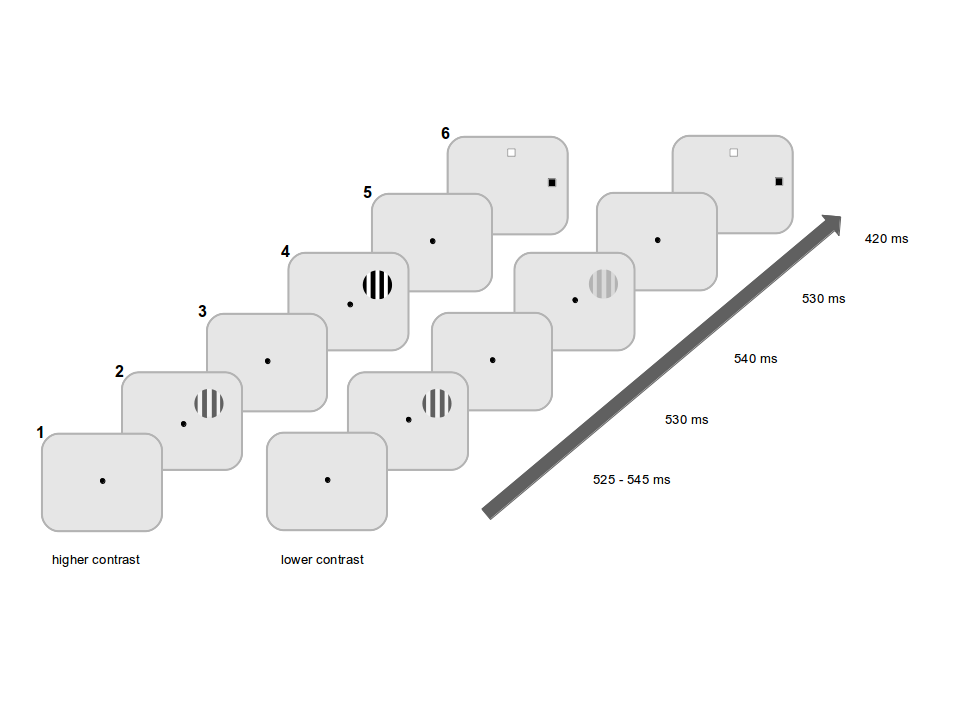
\includegraphics[width=\linewidth]{./figs/PLtask1.png}
\end{center}
\caption{
Experimental procedure.
1:~The monkey fixates upon a central spot. 2:~A sample stimulus in the form of either a Gabor patch or a sine grating is presented at the pedestal contrast (\eg{}~30\%). 3:~Blank sample-test interval. 4:~Test stimulus presented. 5:~Blank test-target interval. 6:~Two target stimuli appear to the left and right of the test stimulus location, signalling that the subject is allowed make a saccade to their chosen target.
Subject's overall objective is to make a comparison between the contrasts of the sample and test stimuli (presented during steps 2 and 4, respectively): if the test stimulus was of a higher contrast (\eg{}~32\%) than the pedestal contrast, they should saccade to the white target, otherwise if the second patch was of lower contrast (\eg{}~28\%), they should saccade to the black target (step 6).
Durations shown are approximates as the actual durations vary slightly depending on the animal: see Table.~\ref{tab:tptimes} for more accurate values.}
\label{fig:pltask1}
\end{figure}

After the monkey has been fixated on the fixation point for a randomised period of time
$t_1$,
a grey-scale Gabor function with a contrast $C_{sample}$ appears on the screen. We refer to this as the \textit{sample stimulus}, and it appears in the animal's field of vision such that it is retinotopic to the location of the implanted brain region.
This Gabor stimulus remains on screen for $t_2$, after which it vanishes.
There follows a delay of $t_3$, during which the animal must continue to fixate on the fixation point.
After this, a second Gabor stimulus with contrast $C_{test}$ appears in the same location as the sample stimulus, also for $t_4$. We refer to this as the test stimulus.
There is then a delay of $t_5$ before the fixation target vanishes and a pair of black and white response target squares appear in a region away from the stimulus location. The monkey is tasked with saccading to the white target if the test stimulus has lower contrast than the sample, or the black target if test has higher contrast. If the monkey responds correctly, it is immediately given a water reward. The experiment is thus a two-alternate forced-choice experiment.
After the animal has given its response, the next trial begins without delay, and the fixation target again appears alone on the screen until the monkey has fixated for some randomised duration $t_1$.
The durations used for each part of the experiment are given in Table.~\ref{tab:tptimes}.

\begin{table}[hbtp]
\caption{Durations of each section of the trials.
$t_1$:~interval from fixation-start until sample presentation.
$t_2$:~sample presentation.
$t_3$:~sample-test stimulus interval.
$t_4$:~test presentation.
$t_5$:~test-targets interval.
Differing monitor refresh rates for the two monkeys results in different durations because stimuli can only be presented at the start of the monitor refresh cycle.
\NB{}~A random duration for $t_3$ was used when the experiment was performed on M1 in V4, but this was changed to a static delay for data collected later.}
\label{tab:tptimes}
\begin{center}
\begin{tabular}{rlr}
\toprule
Animal  & Region & Time ($\unit{ms}$)
% \\
%         &       & Inter-trial delay
\\
\midrule
M1  & V4    & $530.872 \le t_1 \le 545.526$
\\
        & V1    & $525.803 \le t_1 \le 538.983$
\\
M2    & V4    & $526.295 \le t_1 \le 540.641$
\\
        & V1    & $525.834 \le t_1 \le 540.702$
% \\
% \midrule
%         &       & Sample presentation duration
\\
\midrule
M1  & V4    & $t_2 = 529.275$ 
\\
        & V1    & $t_2 = 529.275$
\\
M2    & V4    & $t_2 = 533.176$
\\
        & V1    & $t_2 = 533.176$
% \\
% \midrule
%         &       & Post-sample stimulus delay
\\
\midrule
M1  & V4    & $539.720 \le t_3 \le 1058.673$
\\
        & V1    & $t_3 = 541.164$
\\
M2    & V4    & $t_3 = 546.632$
\\
        & V1    & $t_3 = 546.570$
% \\
% \midrule
%         &       & Test presentation duration
\\
\midrule
M1  & V4    & $t_4 = 529.275$
\\
        & V1    & $t_4 = 529.275$
\\
M2    & V4    & $t_4 = 533.176$
\\
        & V1    & $t_4 = 533.176$
% \\
% \midrule
%         &       & Post-test stimulus delay
\\
\midrule
M1  & V4    & $t_5 = 423.475$
\\
        & V1    & $t_5 = 423.475$
\\
M2    & V4    & $t_5 = 426.578$
\\
        & V1    & $t_5 = 426.640$
\\
\bottomrule
% \toprule
%         &       & Time(ms)
% \\
% Animal  & Brain region & $t_1$  & $t_2$  & $t_3$  & $t_4$   & $t_5$
% \\
% \midrule
% M1  & V4    & $530.872 \le t_1 \le 545.526$   & $t_2 = 529.275$  & $539.720 \le t_3 \le 1058.673$  & $t_4 = 529.275$  & $t_5 = 423.475$
% \\
%         & V1    & $525.803 \le t_1 \le 538.983$   & $t_2 = 529.275$  & $t_3 = 541.164$  & $t_4 = 529.275$  & $t_5 = 423.475$
% \\
% M2    & V4    & $526.295 \le t_1 \le 540.641$   & $t_2 = 529.275$  & $t_3 = 546.632$  & $t_4 = 533.176$  & $t_5 = 426.578$
% \\
%         & V1    & $525.834 \le t_1 \le 540.702$   & $t_2 = 533.176$  & $t_3 = 546.570$  & $t_4 = 533.176$  & $t_5 = 426.640$
% \\
% \bottomrule
\end{tabular}
\end{center}
\end{table}

Following a period of rest after surgery, during which the implants should settle into stable locations, the animals are pre-trained to sit in the chair and fixate on the fixation point. They are then trained in the procedure of the experiment, whilst recordings are taken from V4. Their preliminary training involves a grey disc as the sample, whilst the test is either white or black. This then changes to be a set of Gabor functions.
% check this


After the preliminary training, the main perceptual learning experiment is performed, first for V4, then V1.
In the main experiment, we keep the contrast of the sample as $C_{sample} = 30\%$ throughout.

The test contrast is chosen from a set of 14 contrasts:
\{10, 15, 20, 25, 27, 28, 29, 31, 32, 33, 35, 40, 50, 60\}\% for V1 and
 \{5, 10, 15, 20, 22, 25, 28, 32, 35, 40, 45, 50, 60, 90\}\% for V4,
for both of the animals. These groups are chosen such that the animal has a similar initial accuracy for both V1 and V4. We note that half of the contrasts are above and half below the sample contrast of 30\%.
The contrast is not chosen randomly at the start of each trial; instead a batch of trials containing a set number of each test contrast is placed into sequence all at once.
If the monkey responds incorrectly at the end of the trial, this contrast is added to a list to be repeated at the end of the batch.
At the end of the batch, another batch of trials begins in a similar fashion.
% This \textit{delayed repeat} method is used because ...
%(This will be an important fact later in the study.)

The duration of daily training was typically limited by the animal's desire to preform the task. On some days the animal was reluctant to train at all and only 250 trials could be conducted; whilst on other days the animal would be willing to train for three hours and complete up to 1250 trials.
As expected, the psychometric performance of the monkey increased each day for around 20 days due to perceptual learning. After the performance stayed the same for 5 consecutive days, the experiment progressed to the next stage.


\begin{figure}[htbp]
\begin{center}
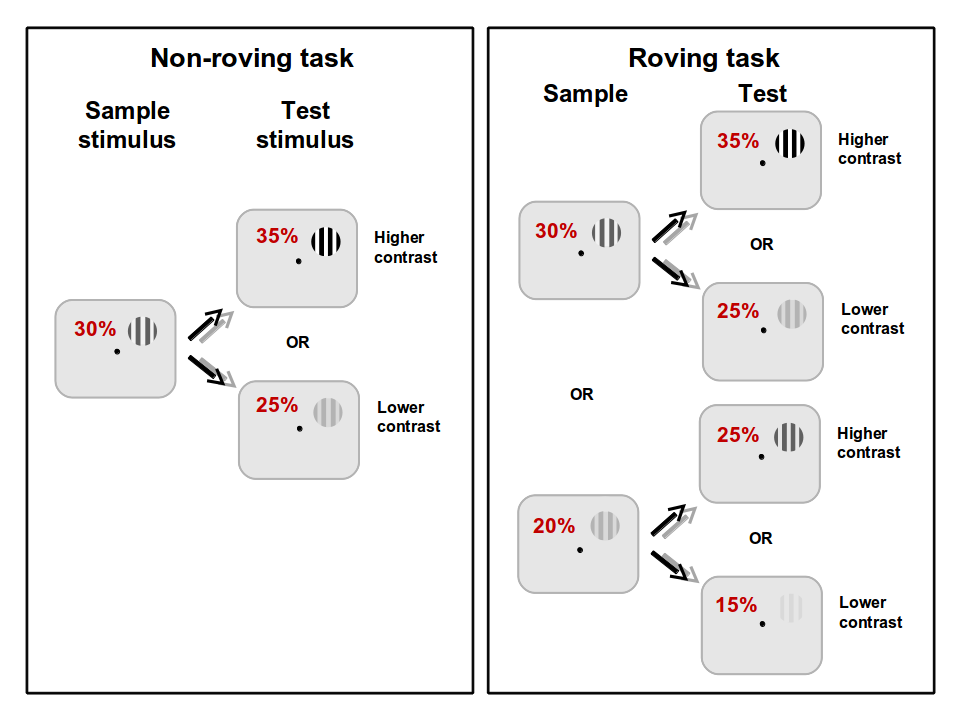
\includegraphics[width=0.8\linewidth]{./figs/PLtask2.png}
\end{center}
\caption{The experimental task during both the non-roving and roving stages. The analysis contained in this report concerns only the first, non-roving, stage.}
\label{fig:pltask2}
\end{figure}

% \begin{figure}[htbp]
% \begin{center}
% 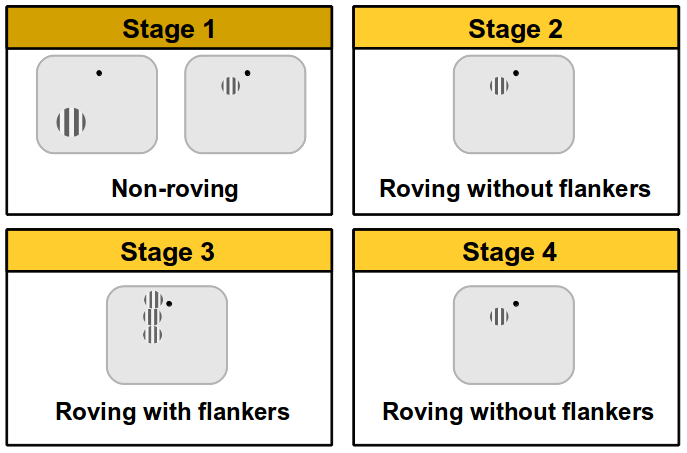
\includegraphics[width=0.8\linewidth]{./figs/PLtask3.png}
% \end{center}
% \caption{The experiment was composed of 4 stages. In this analysis, we are concerned only with the first stage.}
% \label{fig:pltask3}
% \end{figure}

In this study, we will focus on analysing data from the non-roving perceptual learning task as described above. However, it should be noted that once the animals had completed the non-roving stage of the experiment, they progressed to further stages involving a roving task. In the roving task, the sample contrast was chosen at random with $C_{sample} \in \{20, 30, 40\}\%$. Subsequently, once the test stimulus had been shown and the targets appeared, the animal was tasked with responding by comparing the test contrast to whichever sample contrast was presented on that particular trial. During this task, the test contrast would be selected from a set of 12 contrasts specific to each of the three sample stimuli, such that 6 test stimuli were higher and 6 lower in contrast than the sample. The difference between the non-roving and roving stages is illustrated in Fig.~\ref{fig:pltask2}.
%
% One small inconsistency in the experimental setup is that for M1 during the V4-based task, the inter-stimuli wait was chosen randomly as $t_3 \in [x,y]ms$. For later experiments, including the V1 recordings for M1 and both V4 and V1 recordings for M2, the inter-stimuli wait was fixed at $t_3 = z ms$.

As mentioned in Sec.~\ref{sec:bgpl}, some previous research has found flankers around the stimuli are necessary to induce perceptual learning.
During this experiment, the researchers found flankers were not necessary for perceptual learning during the first stage, but to subsequently learn to the roving task, flankers around the stimuli were necessary.

% A related experiment to investigate which neural receptors are important for perceptual learning to take place has been undertaken on a third monkey. This monkey, Frank, has been exposed to neuropharmacological agents to see how they affect perceptual learning; the two agents used are the NMDA-receptor antagonist APV, and the muscarinic and nicotinic receptor antagonist scopolamine.

%----------------------------------------------------------------------------------------------------------------------
% \chapter{Data Analysis}
%----------------------------------------------------------------------------------------------------------------------
\section{Spike-Sorting}
\label{sec:sorting}

The initial intention in this study was to first analyse the pre-filtered continuous data using an automated spike detection and sorting program. The output from the automated sorting would then be used for the main portion of the study and analysed using information theoretic techniques.
The motivation for using an automated spike-sorting program was three-fold.

Firstly, data recordings are collected from an array of intracellular electrodes. After thresholding the continuous data to extract the spikes, we will be left with spikes from a handful of neurons closest to the electrode, with different peak voltages depending on their distance from the recording electrode. Since different not all neurons behave in the same manner, we would like to isolate individual neurons for the following analysis.

Secondly, automated spike-sorting will use the same rules to sort the spikes for every session throughout the experiment, so the results will be very consistent. In comparison to this, sorting spikes manually by eye is subjective, and it is impossible even for the same human to apply exactly the same methodology every time they perform the process.

Thirdly, sorting spikes manually is very time consuming, and not practical to do within the time constraints of this project.

%----------------------------------------------------------------------------------------------------------------------
\subsection{Methods}

Before the project began, a candidate spike-detection and spike-sorting program, \textit{Wave Clus}, was identified.%
\footnote{
\textit{Wave Clus} is available online at
\url{http://www2.le.ac.uk/departments/engineering/research/bioengineering/neuroengineering-lab/spike-sorting}
}

The extracellular voltage recordings include the spikes of any neurons surrounding the microelectrode and background noise (from more distant spikes), on top of the more gradual changes in local field potential (LFP). These voltage recordings have already been low- and high-pass filtered to isolate the voltage signals from the LFP and spikes respectively.

In order to best study the information content of the spiking data, we need to know the spike times of individual neurons \cite{Quiroga2009}. Since each neuron will give a characteristic spike profile in the voltage trace, specific to the type neuron, its intracellular properties, and its distance from the microelectrode, it is possible to group together the spikes which come from the same neurons \cite{Quiroga2007}.
This is done by applying spike-detection and spike-sorting algorithms to the high-pass filtered data.

This method involves spike-detection with a threshold of
$$
%\text{thr}
\theta
= \frac{4}{0.6745} \operatorname{median} \left( |x| \right)
,$$
followed by a wavelet transformation of the spikes, and then superparamagnetic clustering on the 10 wavelet coefficients which provide the maximum variance to group the spikes together for specific neurons~\cite{Quiroga2004}.
In a related paper, Rodrigo Quian Quiroga \etal{} found that in tests with simulated data this method outperforms older techniques such as using PCA for feature extraction and $K$-means for clustering~\cite{Quiroga2004}.

%----------------------------------------------------------------------------------------------------------------------
\subsection{Results}
\label{sec:sorting-result}

It was found that, despite the author's claims of offering a fully automated spike-sorting algorithm, in reality the output from \textit{Wave Clus} needed manual adjustment to merge the neurons sorted at different temperatures during the superparamagnetic clustering into a single set of neurons.

For example, the raw data might contain spikes from 3 different neurons. The software performs superparamagnetic clustering at a variety of temperatures, starting too low (paramagnetic phase) so that all the spikes are clustered together, and ending up too high (ferromagnetic phase) so there are about far too many clusters of spikes, say 50. Inbetween, there is a superparamagnetic phase, in which there are a few clusters each of a reasonable size, and this is where it is hoped that the optimal sorting lies.

However, the superparamagnetic phase spans a wide range of temperatures, so when left completely unsupervised, the software chooses the highest temperature at which a cluster containing more than 60 points appears as the optimal temperature. But this neglects the results from other temperatures in the superparamagnetic region, and it is perfectly plausible that there is one temperature, $T_1$, at which the spikes are clustered in two clusters $C_{1}(T_1)$ and $C_{2}(T_2)$
and another temperature, $T_2$, at which the spikes are clustered in two clusters $C_{1}(T_2)$ and $C_{3}(T_2)$.
The optimal sorting is actually to use three clusters $C_1, C_2, C_3$, but the spikes which belong in these three clusters are not all correct at the same temperature. The user must choose temperature $T_1$, lock the spikes $C_{2}(T_2)$ so they stay there, then move to $T_2$ and let the other spikes move around as appropriate.

The process is somewhat tedious, and not terribly clear.
Furthermore, even if it is not necessary to manually intervene with the clusters, the user is required to check this manually.

Another problem is that the temperatures used during the clustering have to be predefined, and different datasets have different optimal temperatures, so there is no guarantee that the range of temperatures used will find a good sorting of the neurons. Granted, this is an understandable limitation, since it is impractical to endlessly search parameter space, and most of the time the range of temperatures used will be suitable, but it seems that it would not be so difficult to find a good range of temperatures on the fly by checking whether the paramagnetic and ferromagnetic bounds have been found.

In the interests of time and the desire to proceed with the main part of the experiment, the decision was taken to abandon the spike-sorting and use the sortings already performed by the researcher, Xing Chen, who had conducted the experiments. This analysis is presented in the following section.

The recordings were collected and processed using the Neurolynx electrophysiology data recording and processing software suite.
Raw recordings were filtered to include only the frequency band \unit[600--4000]{Hz}, and spikes extracted with a sampling frequency of \unit[32556.000]{Hz}.

The researcher found that for some channels multiple individual neurons could be isolated from the spike-sorting, whilst for many only one neuron was sorted. However, for many of the channels where multiple neurons could be sorted, they could not be reliably sorted for every training session. So for consistency in the analysis over multiple sessions, the spikes from these individual neurons were merged together.

%----------------------------------------------------------------------------------------------------------------------
%----------------------------------------------------------------------------------------------------------------------
%----------------------------------------------------------------------------------------------------------------------
\chapter{Information Theoretic Analysis}
%----------------------------------------------------------------------------------------------------------------------

As mentioned in Sec.~\ref{sec:sorting-result}, the automated spike sorting had to be abandoned. The dataset used in this section consists of spiking activity manually sorted by the researcher who collected the data.

%----------------------------------------------------------------------------------------------------------------------
\subsection{Methods}

To best illustrate the process gone through in the study, we include some preliminary results amongst the methods.
This is presented so the reader will better understand the decisions taken whilst progressing with the analysis.

%----------------------------------------------------------------------------------------------------------------------
\FloatBarrier
\subsubsection{Artifact elimination}
\label{sec:ma}

Looking at rasters generated to include all the trials across all the sessions, an anomaly was apparent.
For several of the channels in the data from each of the brain regions of each of the animals, some sessions have spikes which align at the same time relative to the stimulus onset. The temporal alignment is very precise, indicating the effect not part of the animal's brain activity but instead due to an external source influencing the detected signal in the recordings. Furthermore, the ``lines'' occurred at regularly spaced intervals, with a period very nearly equal to the refresh rate of the monitor. The spikes across multiple trials line up like this because the experimental equipment will only begin presenting a stimulus when the first pixel on the monitor is being updated, and we of course normalise for the stimulus presentation time across multiple trials.
% INCLUDE RASTER EXAMPLE

An empirical estimate of the artifact periodicity was found by choosing an arbitrary channel which strongly expresses the artifact and measuring by eye the duration of the completed artifact cycles within \unit[530]{ms} (44 for M1, 39 for M2). Since the artifact is tightly localised in time, this could be done with relatively high accuracy. For M1, the period was estimated to be \unit[85.023(1)]{Hz}, whilst for M2 it was \unit[75.023(1)]{Hz}. The discrepancies from the programmed monitor refresh rates of \unit[85]{Hz} and \unit[75]{Hz} respectively can be put down to the specific electronic circuitry used, perhaps issuing the command to the monitor. The discrepancy is small enough to be of little consequence, except we will need \unit[5]{sf} of accuracy rather than \unit[2]{sf} in the following treatment of the artifact. Why it should be out by exactly \unit[0.023]{Hz} for both animals remains unclear, since this corresponds to the refresh cycle running \unit[0.0031]{ms} fast for M1 and \unit[0.0042]{ms} fast for M2. An even bigger mystery is how the artifact has made its way into the recordings. Although it remains possible that the cause is some other piece of equipment also locked to the same refresh cycle, in the following we will refer to this artifact as the ``monitor artifact''. When a collection of datapoints exhibits the monitor artifact, we refer to the data as ``contaminated''.

From the rasters, it seemed as if three-quarters of the channels in M1 V4 were contaminated for at least one session; over two-thirds of the channels for M1 V1 and M2 V4 were contaminated for at least one session; and around a third of the channels for M2 V4 were contaminated for at least one session. The contaminated channels include both high-quality channels with a lot of detected spikes, and low-quality channels with fewer detected spikes. For some of the lowest quality channels and sessions, the artificial spikes were clearly more numerous than the genuine ones. It was considered paramount that the effects of the artifact be corrected for.

To clean up the contamination, a more rigorous method of evaluating the problem was required.
For the collection of spike times from a single channel across multiple trials during a single session, we perform the following steps:
\begin{enumerate}
\item Consider the set of all spiketimes where the visual stimulus has been the same for at least the last \unit[150]{ms}.
\item From each spiketime, $t$, subtract time of nearest stimulus onset/offset, $T_{\text{onset}}$. (Both onset and offset are synchronised with the monitor cycle, and the nearest one offers greatest accuracy.)
$$
t \leftarrow t - T_{\text{onset}}
$$
\item Take the modulo of the spiketimes with respect to the monitor period, $\tau_m$ (\unit[11.7616]{ms} for M1, \unit[13.3292]{ms} for M2).
$$
t \leftarrow t \bmod \tau_m
$$
\item Take a histogram of the spiketimes over bins with the width of the reciprocal of the sampling frequency of the spikes (sampling frequency \unit[32556.000]{Hz}; bin width \unit[0.030716]{ms}).
\end{enumerate}
Conceptually, this is equivalent to stacking all the ``lines'' in the raster on top of each other and seeing how thick the resulting line is.
When the visual stimulus has remained unchanged for at least \unit[150]{ms}, the neurons in V1 and V4 settle down to a steady firing rate, so we expect there to be about the same number of spikes in each of these bins. However, as the monitor artifact increases the number of spikes at set intervals after the monitor refresh commences, there will be an increase in the number of spikes in these bins when the monitor artifact is manifest in the data.

% ./figs/monitor_hist_blanco_v4_ch4_s336_20120817T085037.eps
% ./figs/monitor_hist_jack_v1_ch9_s51_20120817T084845.eps
% ./figs/monitor_hist_jack_v1_ch9_s56_20120817T084855.eps
% ./figs/monitor_hist_jack_v4_ch41_s31_20120817T085111.eps
%%\begin{figure}[htbp]
%%    \begin{subfigure}[b]{0.5\linewidth}
%%        \centering
%%        \caption{}
%%        \label{fig:mahist-b4}
%%        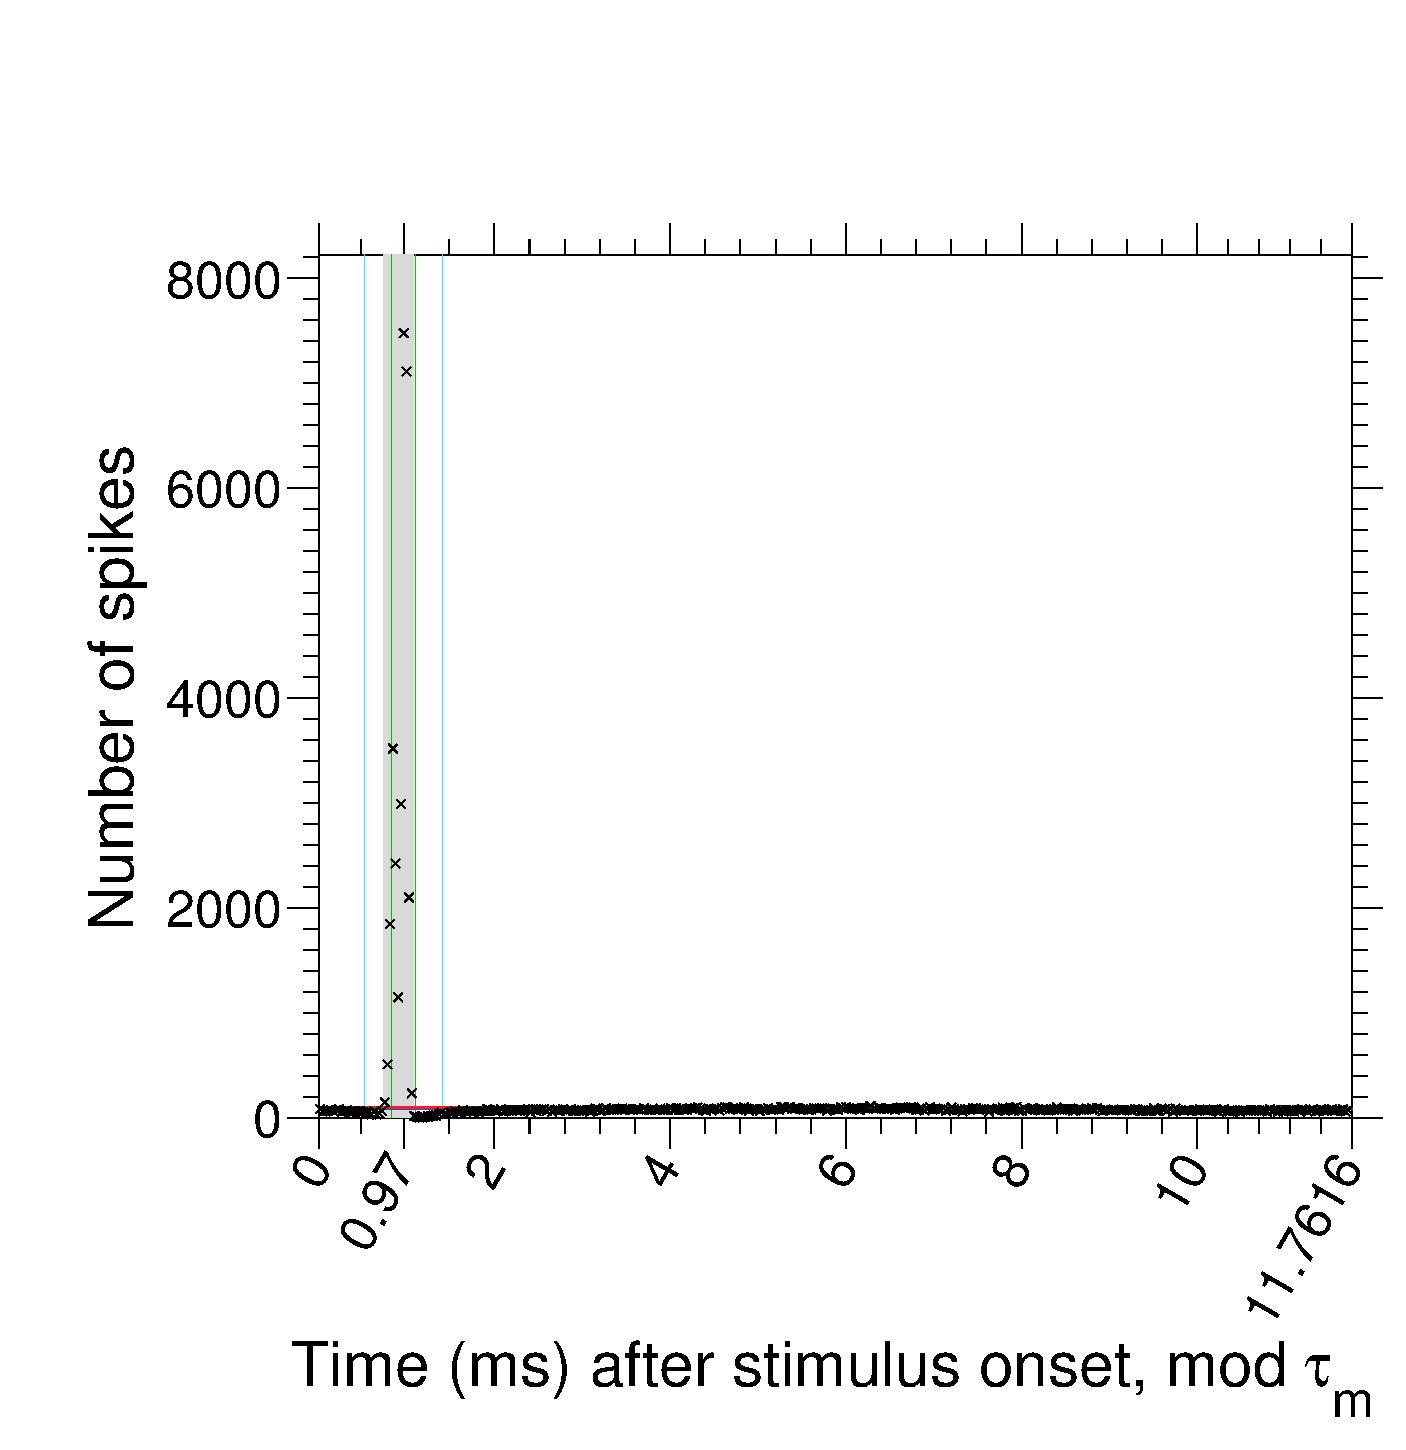
\includegraphics[width=\linewidth]{%
%%./figs/monitor_hist_blanco_v4_ch4_s336_20120817T085037.eps}
%%    \end{subfigure}
%%    ~~
%%    \begin{subfigure}[b]{0.5\linewidth}
%%        \centering
%%        \caption{}
%%        \label{fig:mahist-j4}
%%        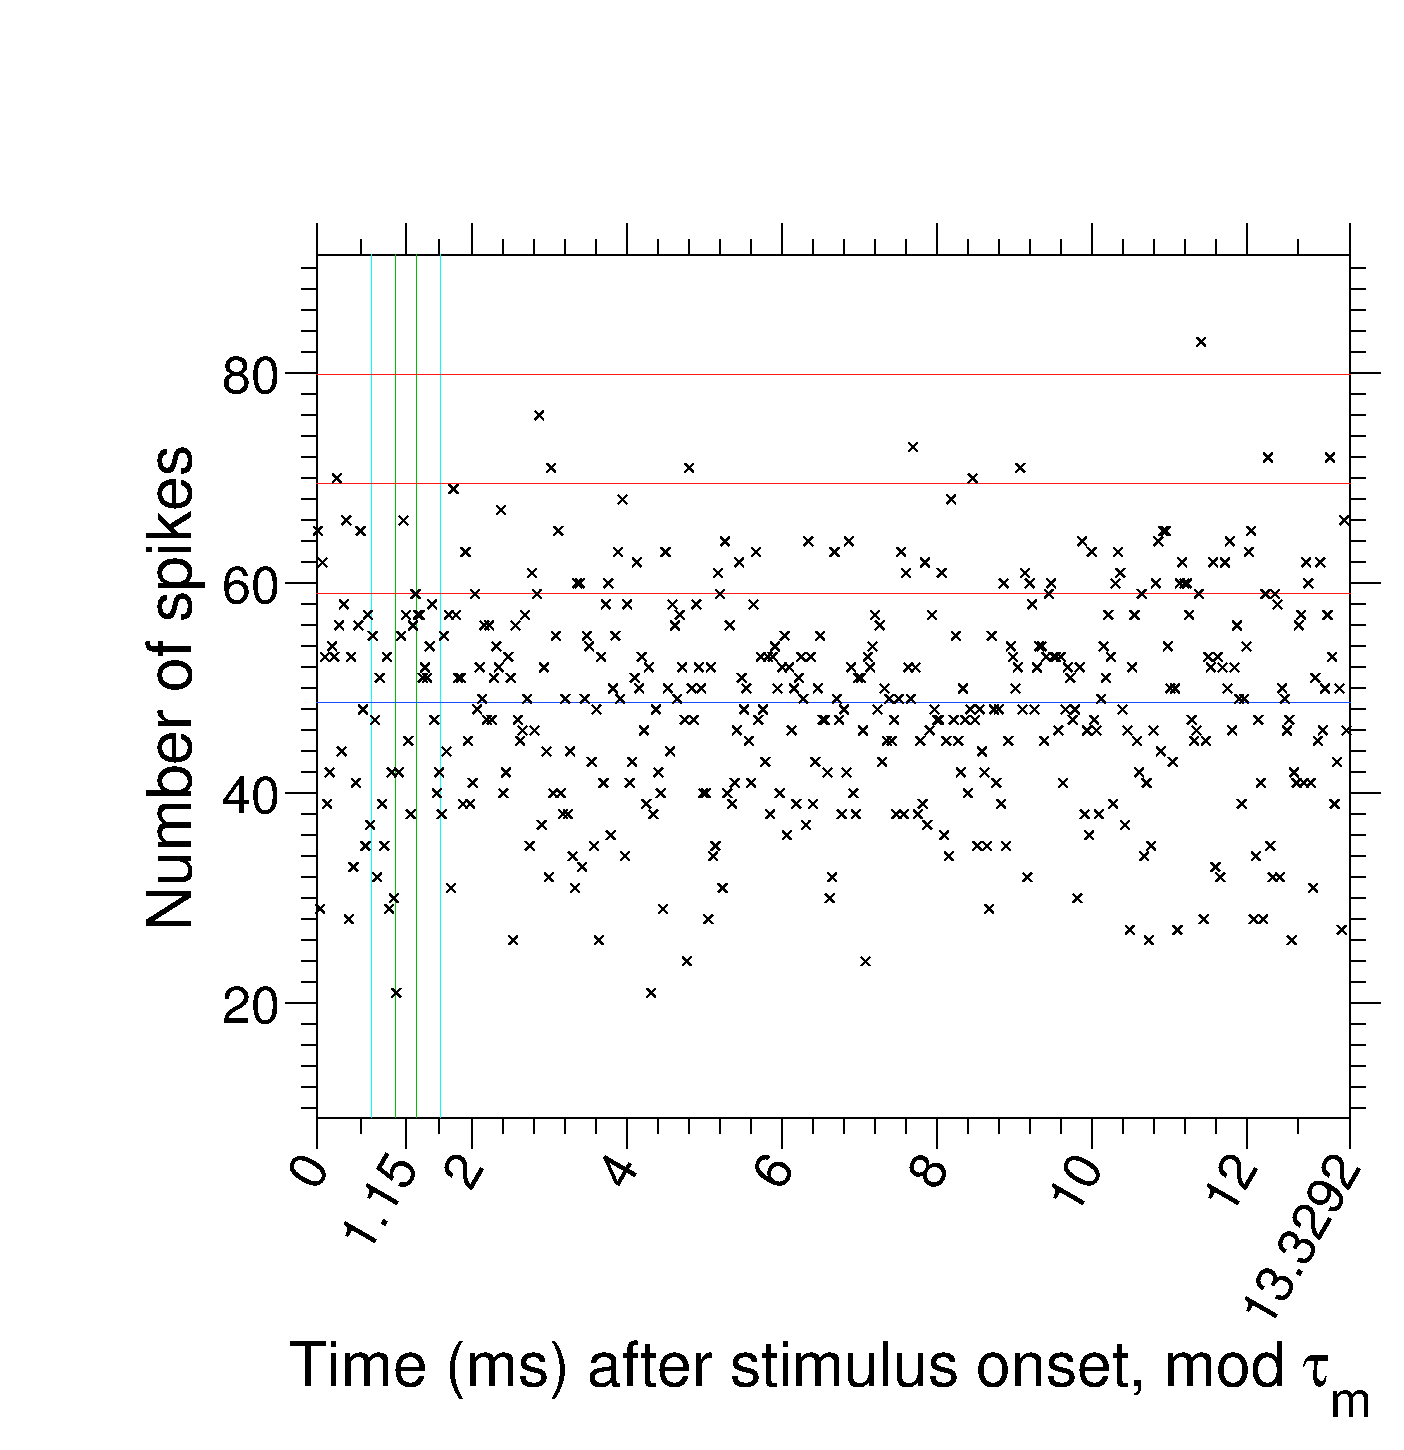
\includegraphics[width=\linewidth]{%
%%./figs/monitor_hist_jack_v4_ch41_s31_20120817T085111.eps}
%%    \end{subfigure}
%%    \\
%%    \begin{subfigure}[b]{0.5\linewidth}
%%        \centering
%%        \caption{}
%%        \label{fig:mahist-j1s51}
%%        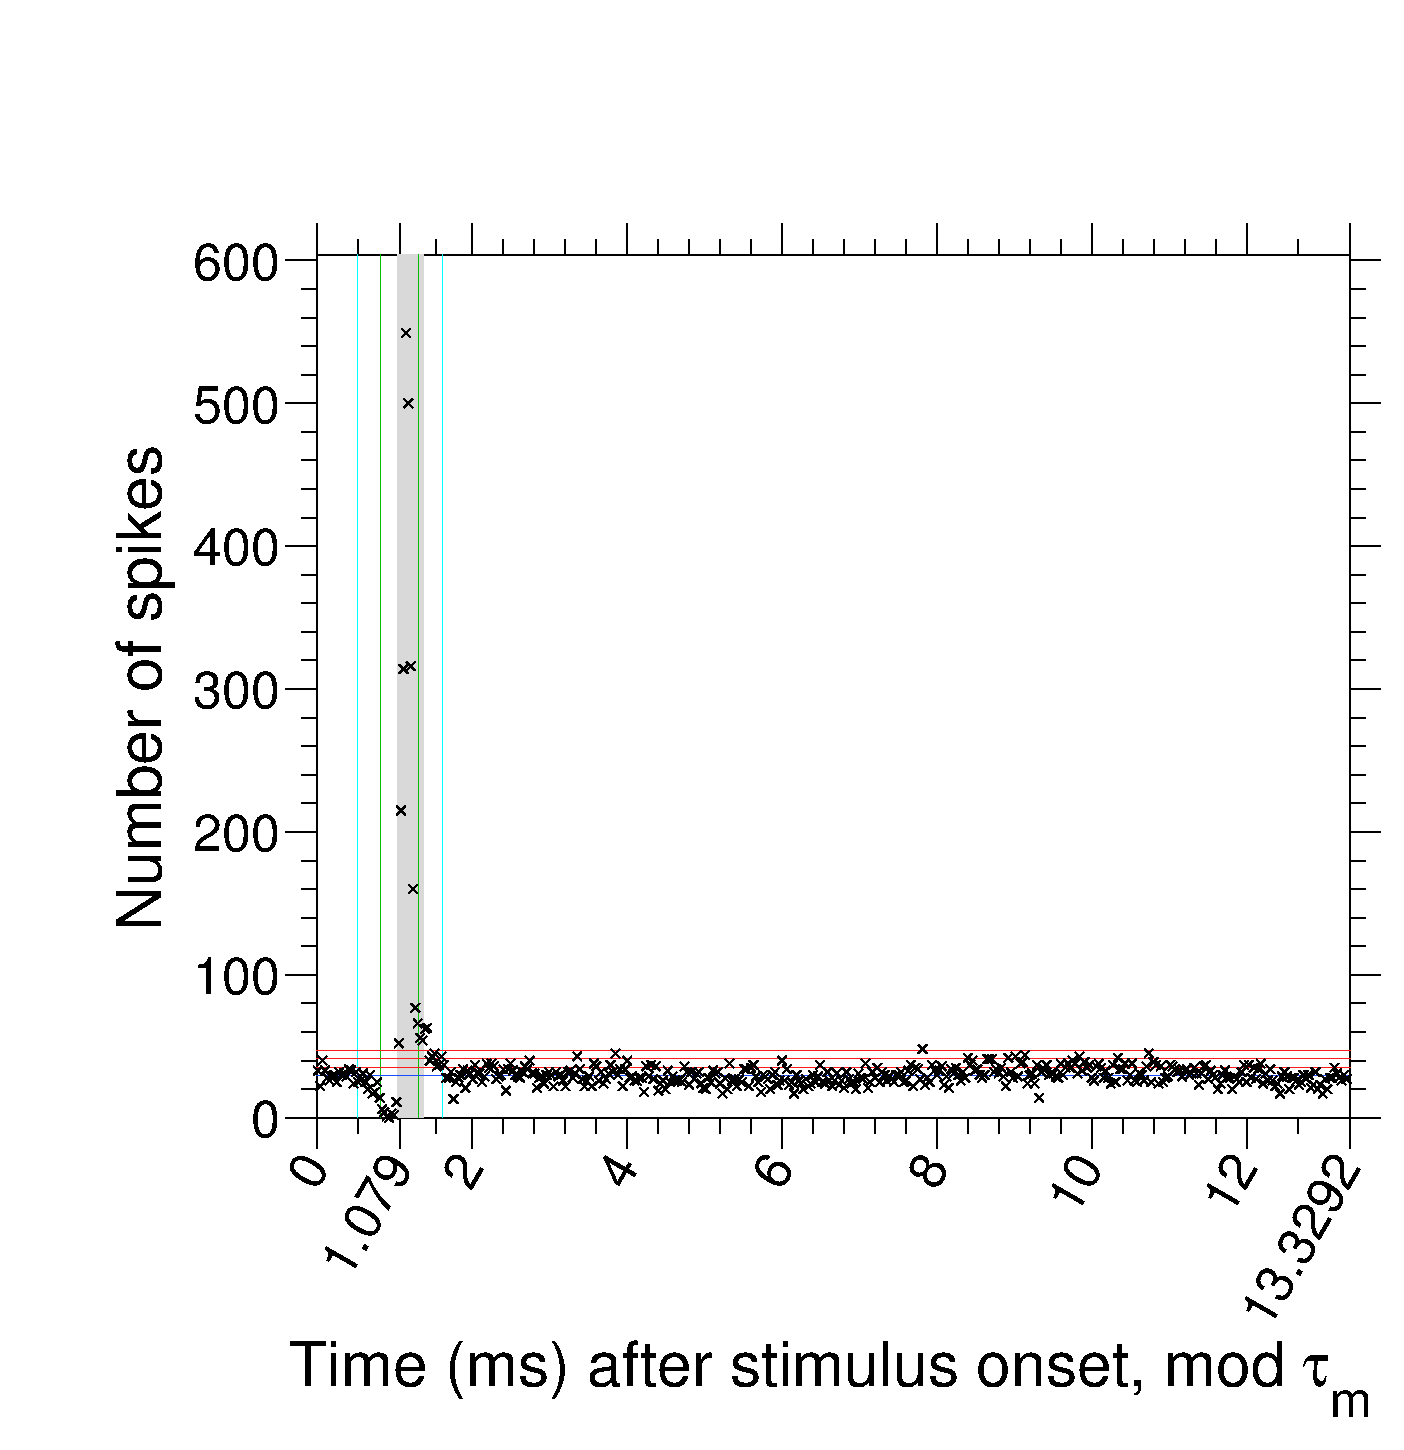
\includegraphics[width=\linewidth]{%
%%./figs/monitor_hist_jack_v1_ch9_s51_20120817T084845.eps}
%%    \end{subfigure}
%%    ~~
%%    \begin{subfigure}[b]{0.5\linewidth}
%%        \centering
%%        \caption{}
%%        \label{fig:mahist-j1s56}
%%        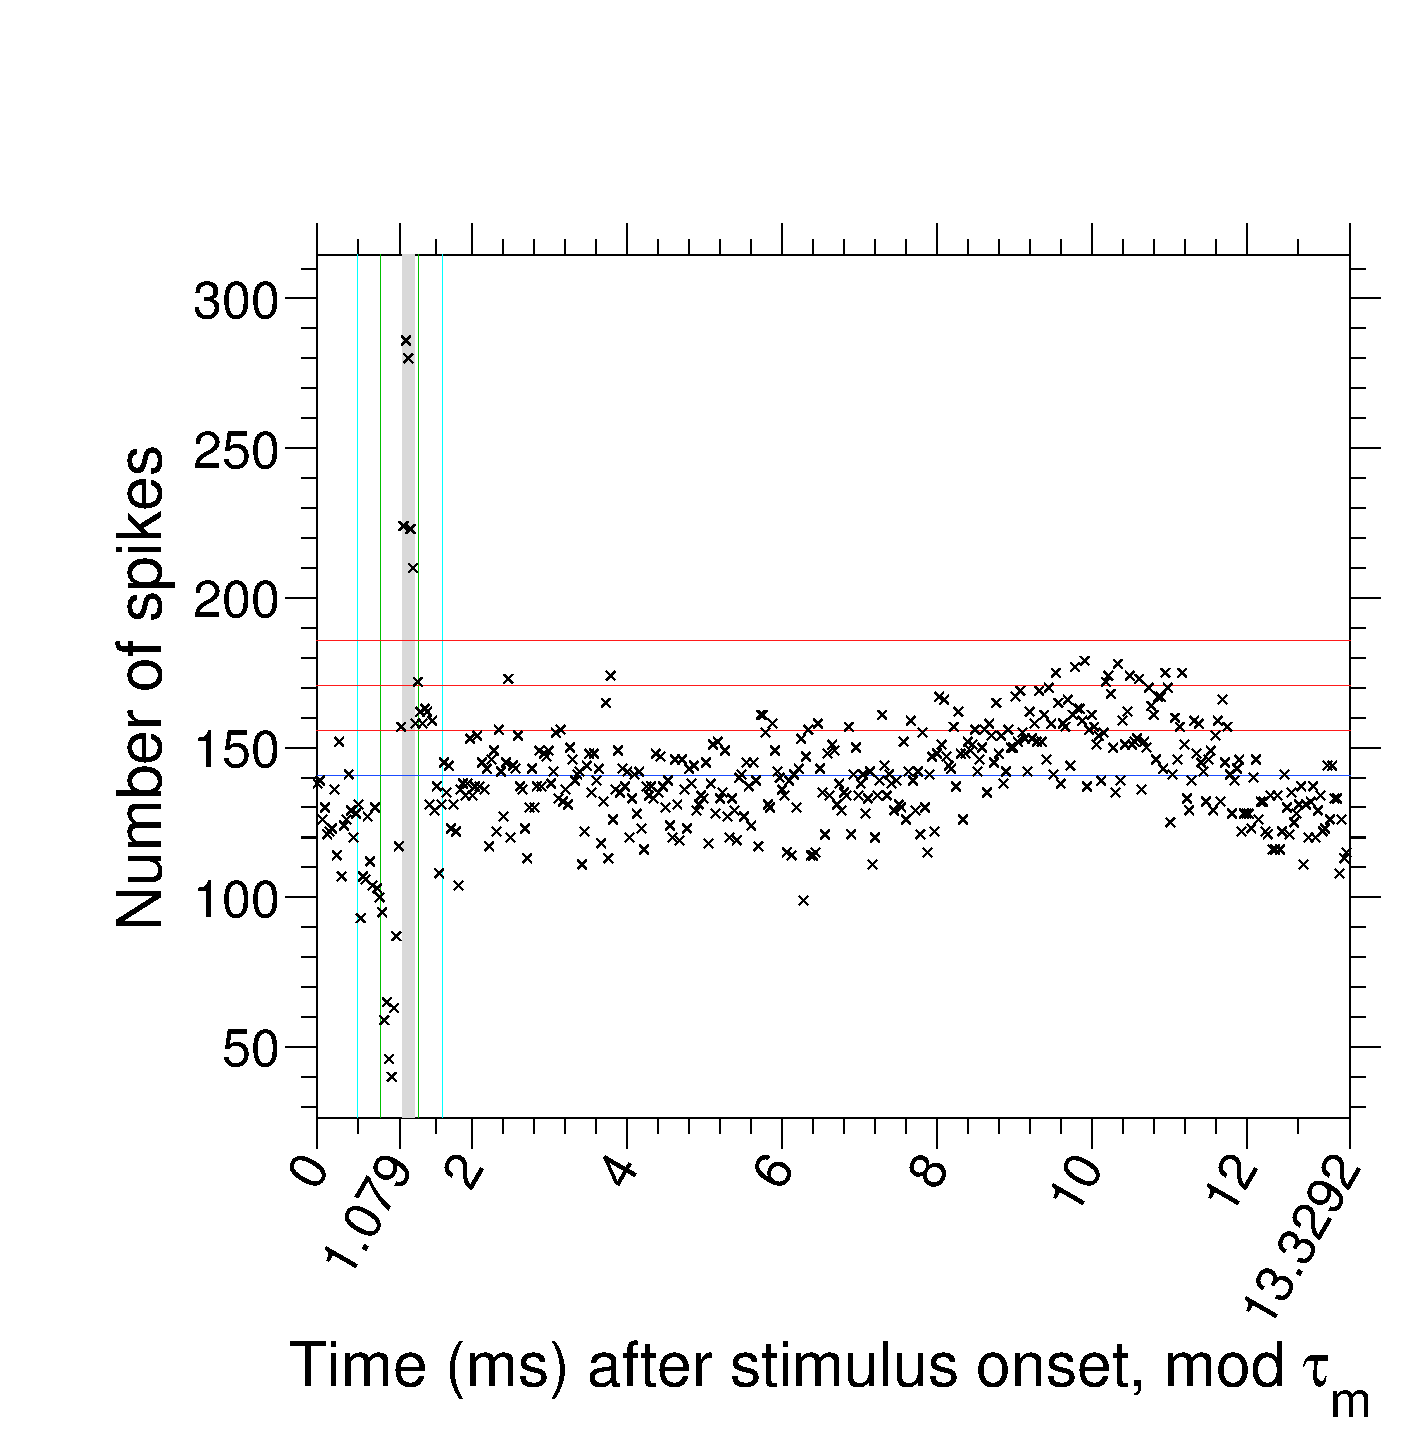
\includegraphics[width=\linewidth]{%
%%./figs/monitor_hist_jack_v1_ch9_s56_20120817T084855.eps}
%%    \end{subfigure}
%%    \caption{Crosses: Histogram of spikes in bins of width \unit[0.030716]{ms}.
%%\ref{fig:mahist-b4}: M1 V4, channel 4, session 336; a channel and session very strongly exhibiting the monitor artifact.
%%\ref{fig:mahist-j4}: M2 V4, channel 41, session 31; a dataset where the artifact is not present.
%%\ref{fig:mahist-j1s51}: M2 V1, channel 9, session 51; data strongly presenting the monitor artifact.
%%\ref{fig:mahist-j1s56}: M2 V1, channel 9, session 56; data mildly showing the effect of the monitor artifact.
%%Green vertical lines: extremities of search window (contained between the lines).
%%Cyan vertical lines: extremities of mean region.
%%Blue line: mean of the data (excluding area between cyan lines).
%%Red lines: mean plus 1, 2 and 3 standard deviations respectively.
%%Gray background: Spikes marked as contaminated and scheduled for redaction.
%%}
%%    \label{fig:mahist}
%%\end{figure}

% INSERT HIST FIGURE 

As shown in Fig.~\ref{fig:mahist}, the analysis conforms to our expectations.
However, doing the analysis in this more rigorous manner revealed the contamination was more widespread than previously assumed. The histograms of spiketimes indicate that more sessions are contaminated than not, and only a couple of channels are completely clean for every session.

For the most part, the timing of the monitor artifact $\bmod \tau_m$ is very reliable and it affects the same 6 or so bins whenever the data is contaminated. The contaminated part of each monitor cycle is thus restricted to at most \unit[0.2]{ms}, and, assuming this period of time contains both genuine spikes and artificial spikes, if we simply delete all datapoints with this \unit[0.2]{ms} window, we will lose at most less than 2\% of the genuine spikes. This level of data loss is not terribly significant, and justifiable for the gain in reliability of the remaining dataset, particularly for sessions where artificial spikes seem to be more common than genuine ones.

\begin{table}[hbtp]
\caption{Typical time of the peak in number of spikes due to the monitor artifact effect. The time is given relative to the start of the monitor refresh as given by the stimulus onset times. Monitor artifacts occur at $t = t^*_m + k \tau_m$, for $k \in \Z$. For channels recording from M2 V1, the artifact will occur at one of the two stated times throughout a given session, but which of the two varies from channel-to-channel for any individual session, and from session-to-session for any individual channel. Why this happens is unclear.}
\label{tab:mapeak}
\begin{center}
\begin{tabular}{rlc}
\toprule
Animal  & Region & Time of artifact peak $t^*_m$ $\pm 0.01$ (\unit{ms})
\\
\midrule
M1  & V1    & 0.95
\\
        & V4    & 0.97
\\
M2    & V1    & either 0.97 or 1.19
\\
        & V4    & 1.15
\\
\bottomrule
\end{tabular}
\end{center}
\end{table}

% However it is apparent that this method is not great (see jack v1 ch7 s57)

However, it is possible to do better that this and to isolate and remove only the contaminated bins. As shown in Fig.~\ref{fig:mahist}, the effect of the artifact is greater for some sessions than others and
From observations on the typical width time of the width and peak time (Table.~\ref{tab:mapeak}) of the artifact, along with its periodicity ($\tau_m$), the following method of removal was devised and implemented.
\begin{enumerate}
\item Perform the modulo $\tau_m$ and take the histogram as described above.
\item Define the ``search region'' as bins which contain spike within $t^*_m \pm \unit[0.130]{ms}$, so we have one bin more than the anticipated artifact width in either direction. (For M2 V1, we use the range \unit[$(0.968 - 0.130 , 1.190 + 0.130)$]{ms}.)
\item Find the mean, $\mu$, and standard deviation, $\sigma$, of all the bins which are at least 10 away (\unit[0.3]{ms} away) from the search region. We also exclude the final bin since $0.030716 \bmod \tau_m \neq 0$ and it is only part-full.
\item If any one of the bins in the search region exceeds $\mu + 3 \sigma$, we declare the session contaminated and proceed with the following steps. If not, it is declared intact and left as it is.
\item All bins in the search region which contain more than $\mu + 3 \sigma$ spikes are declared contaminated.
\item Let $t_m$ denote the time of the centre of the bin in the search region containing the most spikes.
\item All bins which contain spikes within $t_m \pm \unit[0.1]{ms}$ are placed in ``quarantine''.
\item All quarantined bins which contain more than $\mu + 2.5 \sigma$ spikes are declared contaminated.
\item All bins between the first and last contaminated bins are declared contaminated.
\item Consider immediate neighbours of the first bin and if they are also contain more than $\mu + 2.5 \sigma$ spikes, they are declared contaminated.
\item Repeat the above step until either a neighbour is found which is not contaminated, or until a maximum of three bins have been added to the contaminated region.
\item Consider immediate neighbours of the last bin and if they are also contain more than $\mu + 2.5 \sigma$ spikes, they are declared contaminated.
\item Repeat the above step until either a neighbour is found which is not contaminated, or until a maximum of three bins have been added to the contaminated region.
\item Consider the full dataset of spikes for this particular channel and session.
\item For each spike, consider which bin its spiketime would be arranged into.
\item If it is a contaminated bin, the spike is removed from the dataset.
\end{enumerate}

This allows us to have prior assumptions about the location and width of the monitor artifact effect, but be flexible about exactly where it falls and which sets of bins are affected.
It is possible that the dynamically targeted removal method may cause issues due to inconsistency in the data across different sessions, but there is a clearly a gain in the amount of preserved data and a gain in the reliability of the data which remains.

%----------------------------------------------------------------------------------------------------------------------
\FloatBarrier
\subsubsection{Session-based analysis}

merged all neurons together for a single channels

Neurolynx NSE files were loaded into MATLAB using the Neurolynx supplied code when operating on Windows, and an version 6 of an unofficial port for Linux (recommended by Neurolynx) otherwise.%
\footnote{Available at
\\ \url{http://www.urut.ch/new/serendipity/index.php?/pages/downloads.html}}

The information was computed for each day of training (hereafter referred to as a session), for each of the channels from which recordings were available. To gauge the typical behaviour of a neuron, the mean was taken over all the channels.
The mutual information between the spiking activity during test presentation and the identity of the test stimulus was computed
using a spike-timing based code.
This computation was done using the \verb|information| function from the freely available Information Break-down Toolbox \cite{Magri2009} for MATLAB.%
\footnote{Available at \url{http://www.ibtb.org}}

A moving window of $\unit[20]{ms}$ was taken and subdivided into 5 sequential bins, each of $\unit[4]{ms}$.
The number of spikes within each of the 5 bins was totalled up to provide a code letter for the bin.
The combination of the 5 sequential counts forms a codeword.

This is performed across all the trials in a session with the $\unit[20]{ms}$ window placed with the same offset relative to the test stimulus onset.
By assembling the trials according to their test contrast, the mutual information between the contrast and the spiking activity in this window can be computed.

Following the methods employed by the research group, only trials in which the monkey responded correctly were used for this analysis.

%----------------------------------------------------------------------------------------------------------------------
% 5bins of 4ms
% ./figs/I_sessionwise_blanco_v1_chmean23_s343-359_oc1_5bins_of_4ms_dr_naive_pcolorhot_20120815T150057.png
% ./figs/I_sessionwise_blanco_v4_chmean31_s307,308,311,313,314,317,318,320,321,329-341_oc1_5bins_of_4ms_dr_naive_pcolorhot_20120815T150100.png
% ./figs/I_sessionwise_jack_v1_chmean25_s51-72_oc1_5bins_of_4ms_dr_naive_pcolorhot_20120815T150049.png
% ./figs/I_sessionwise_jack_v4_chmean20_s24-49_oc1_5bins_of_4ms_dr_naive_pcolorhot_20120815T150053.png
% 1 bin of 20ms
% ./figs/I_sessionwise_blanco_v1_chmean23_s343-359_oc1_1bins_of_20ms_dr_naive_pcolorhot_20120815T190833.png
% ./figs/I_sessionwise_blanco_v4_chmean31_s307,308,311,313,314,317,318,320,321,329-341_oc1_1bins_of_20ms_dr_naive_pcolorhot_20120815T190836.png
% ./figs/I_sessionwise_jack_v1_chmean25_s51-72_oc1_1bins_of_20ms_dr_naive_pcolorhot_20120815T190825.png
% ./figs/I_sessionwise_jack_v4_chmean20_s24-49_oc1_1bins_of_20ms_dr_naive_pcolorhot_20120815T190829.png
% 
% ./figs/I_sessionwise_blanco_v1_chmean23_s343-359_oc1_5bins_of_4ms_dr_naive_pcolorhot_20120815T202102.png
% ./figs/I_sessionwise_blanco_v4_chmean31_s307,308,311,313,314,317,318,320,321,329-341_oc1_5bins_of_4ms_dr_naive_pcolorhot_20120815T202106.png
% ./figs/I_sessionwise_jack_v1_chmean25_s51-72_oc1_5bins_of_4ms_dr_naive_pcolorhot_20120815T202053.png
% ./figs/I_sessionwise_jack_v4_chmean20_s24-49_oc1_5bins_of_4ms_dr_naive_pcolorhot_20120815T202058.png


%%\begin{figure}
%%\centering
%%\subfloat[A big tikz picture.\label{fig:one}]{%
%%  \makebox[\textwidth][l]{% %%% as above
%%  \resizebox{.45\largefigure}{!}{%
%%    \input{fig/tikzfile}}}}%
%%\hfill%
%%\subfloat[Another big tikz picture.\label{fig:two}]{%
%%  \makebox[\textwidth][l]{% %%% as above
%%  \resizebox{.45\largefigure}{!}{%
%%    \input{fig/tikzfile}}}}%
%%\caption{Two tikz pictures}
%%\label{fig:label}
%%\end{figure}
%%
%%\begin{figure}%
%%\centering
%%\subfloat[][]{...figure code...}%
%%\qquad
%%\subfloat[][]{...figure code...}%
%%\caption{Here are the first two figures of a continued figure.}%
%%\label{fig:cont}%
%%\end{figure}

\begin{figure}[htbp]%
    \centering
    \subfloat[][M1 V1.\label{fig:sessb1}]{%
        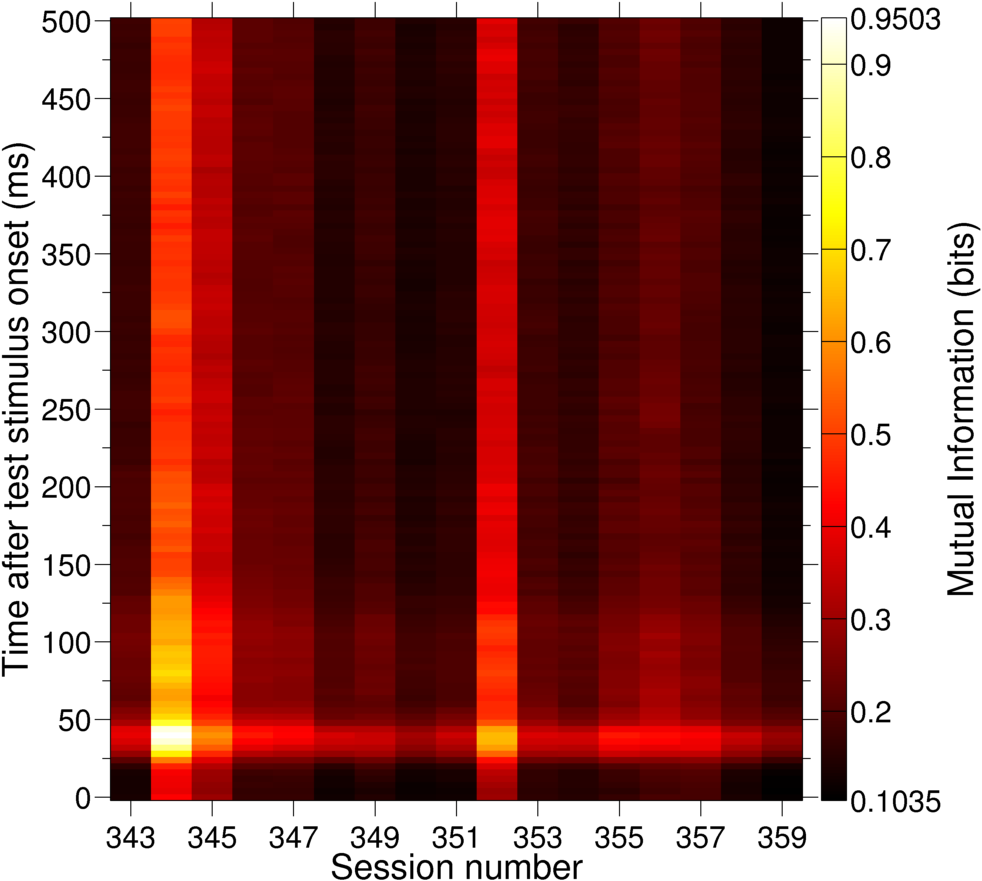
\includegraphics[scale=.25]{%
./figs/I_sessionwise_blanco_v1_chmean23_s343-359_oc1_5bins_of_4ms_dr_naive_pcolorhot_20120815T202102.png}
    }%
    ~~
    \subfloat[][M1 V4.\label{fig:sessb4}]{%
        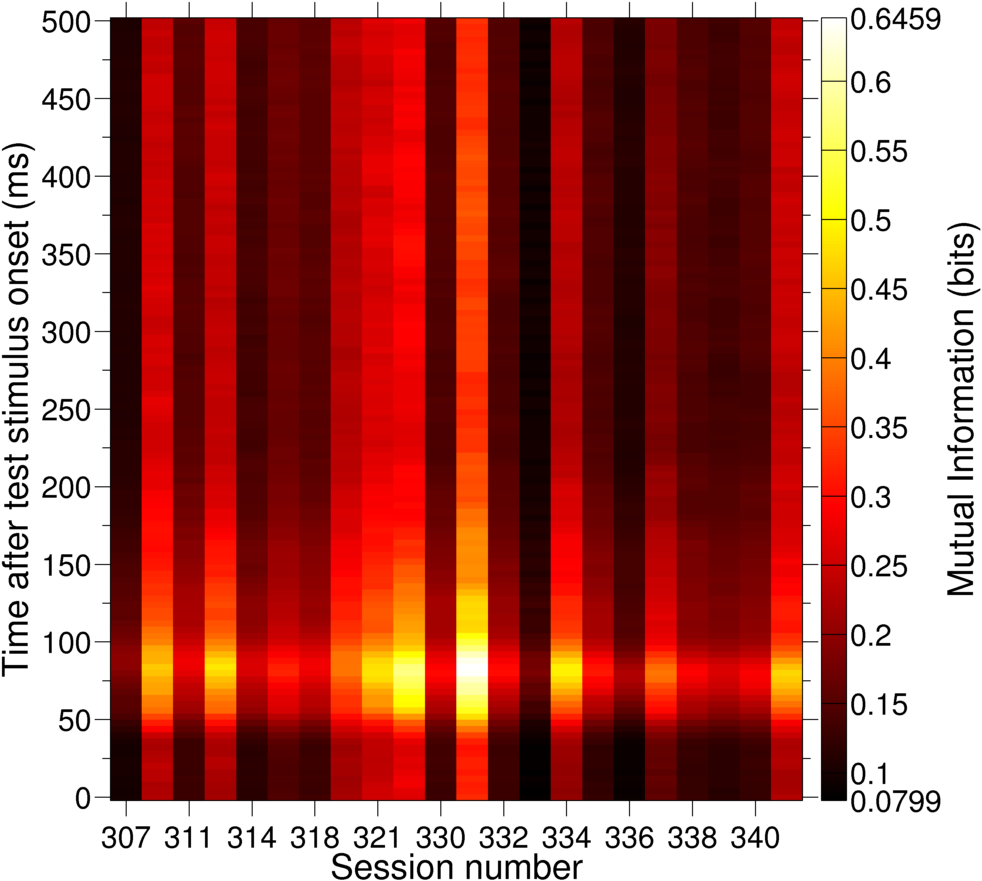
\includegraphics[scale=.25]{%
./figs/I_sessionwise_blanco_v4_chmean31_s307,308,311,313,314,317,318,320,321,329-341_oc1_5bins_of_4ms_dr_naive_pcolorhot_20120815T202106.png}
    }%
    \\
    \subfloat[][M2 V1.\label{fig:sessj1}]{%
        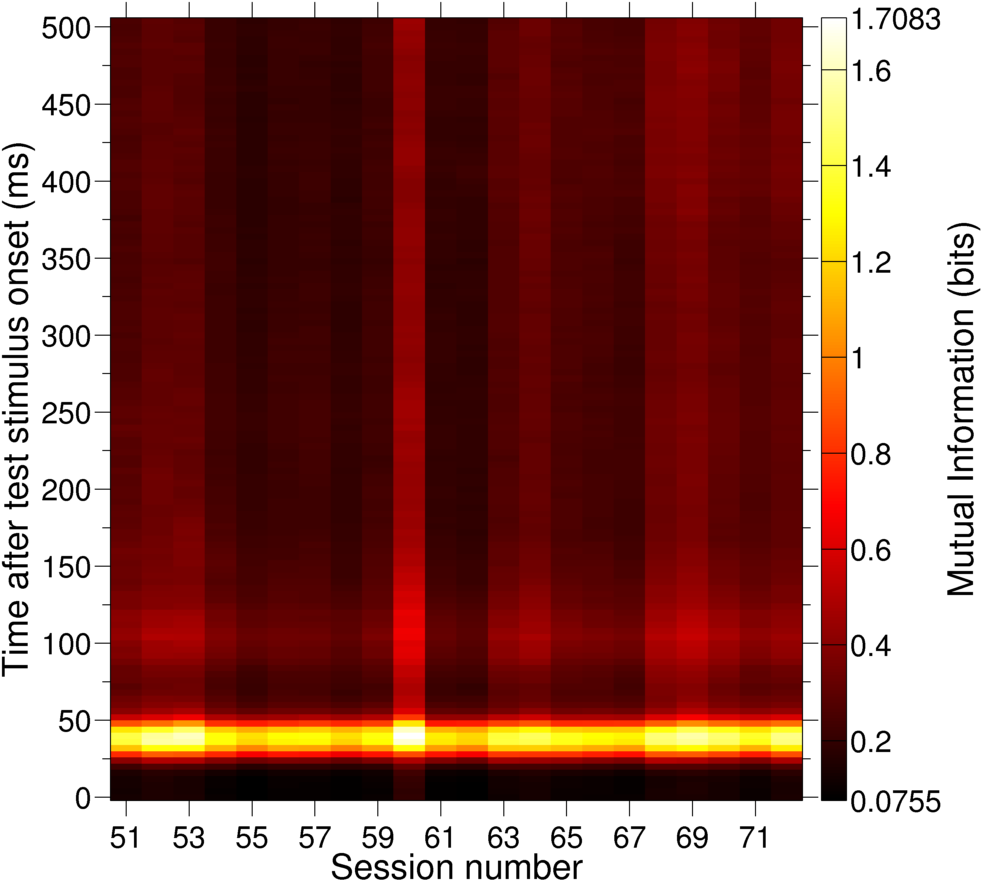
\includegraphics[scale=.25]{%
./figs/I_sessionwise_jack_v1_chmean25_s51-72_oc1_5bins_of_4ms_dr_naive_pcolorhot_20120815T202053.png}
    }%
    ~~
    \subfloat[][M2 V4.\label{fig:sessj4}]{%
        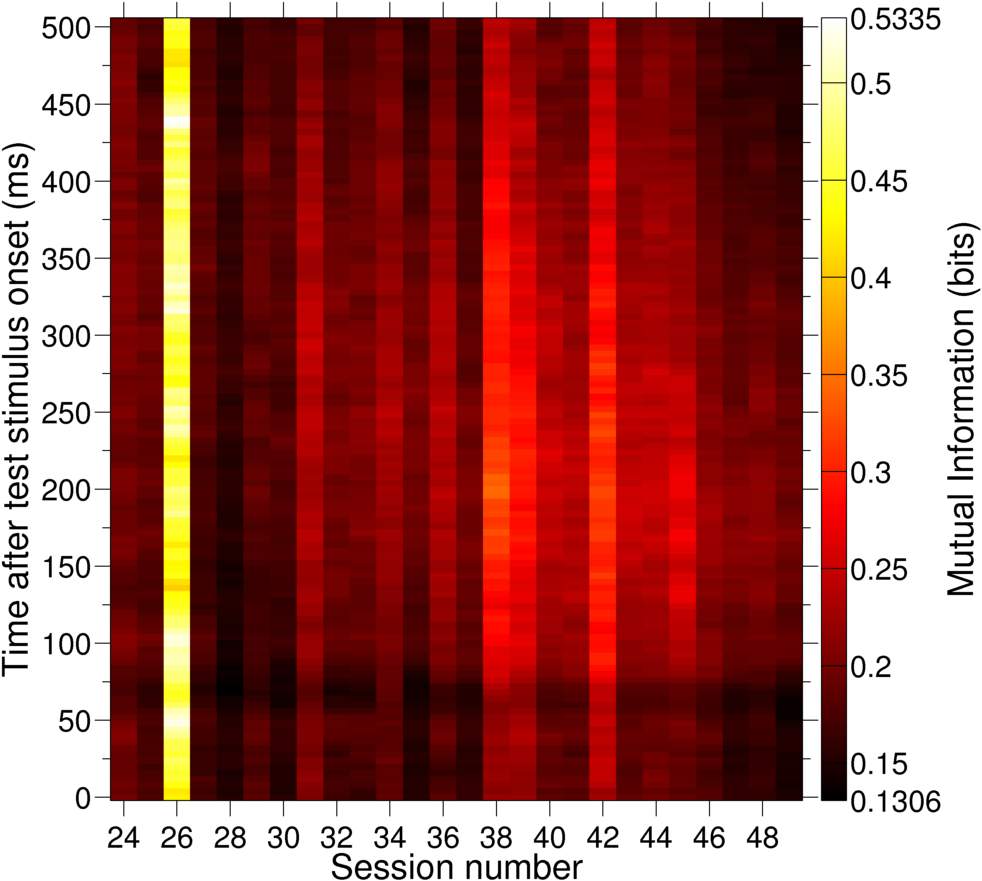
\includegraphics[scale=.25]{%
./figs/I_sessionwise_jack_v4_chmean20_s24-49_oc1_5bins_of_4ms_dr_naive_pcolorhot_20120815T202058.png}
    }%
    \caption{Mutual information between the test stimulus and the neural activity during test presentation.
The mutual information with the test stimulus is taken for a spike timing based code for a \unit[20]{ms} window of spiking activity, sampled with the start of the window offset ($y$-axis) from \unit[0]{ms} up to \unit[500]{ms} after test stimulus onset (which is slightly more than \unit[20]{ms} before test stimulus offset). The sampling is in intervals of \unit[5]{ms}, so any 4 adjacent squares within each session are highly correlated.
The recording session number for the data is given along the $x$-axis, and the number of days the animal has been trained for increases from left to right.
Average mutual information across all the channels is denoted by the pseudo-colour of each of the rectangular patches, centred around the $(x,y)$ co-ordinate to which the measurement relates.
In each case the average is taken across all available channel data: \ref{fig:sessb1}~23 channels, \ref{fig:sessb4}~30 channels, \ref{fig:sessj1}~25 channels, \ref{fig:sessj4}~20 channels.
% The PT bias correction method was used (see text).
The plug-in method without bias correction was used (see text).
}
    \label{fig:sess}
\end{figure}

% ./figs/I_sessionwise_blanco_v1_chmean23_s343-359_oc1_5bins_of_4ms_dr_pt_pcolorhot_20120811T130028.eps
% ./figs/I_sessionwise_blanco_v4_chmean31_s307,308,311,313,314,317,318,320,321,329-341_oc1_5bins_of_4ms_dr_pt_pcolorhot_20120811T130522.eps
% ./figs/I_sessionwise_jack_v1_chmean25_s51-72_oc1_5bins_of_4ms_dr_pt_pcolorhot_20120811T130003.eps
% ./figs/I_sessionwise_jack_v4_chmean20_s24-49_oc1_5bins_of_4ms_dr_pt_pcolorhot_20120811T133212.eps

The results of this initial analysis are shown in Fig.~\ref{fig:sess}.
% Although the relationship between different window offsets and the mutual information is similar for each of the sessions, the
No trend in information content with learning can be discerned because the measured mutual information content varies wildly from session-to-session.

% %----------------------------------------------------------------------------------------------------------------------
% \chapter{}
% %----------------------------------------------------------------------------------------------------------------------
% \subsection{Methods}


% Demonstrate how this is dominated by the number of trials in the session, regardless of bias correction technique

% ./figs/ntrialsIbyNindiv_blanco_v1_dr_naive_20120812T164553.eps
% ./figs/ntrialsIbyNindiv_blanco_v4_dr_naive_20120812T164553.eps
% ./figs/ntrialsIbyNindiv_jack_v1_dr_naive_20120812T164553.eps
% ./figs/ntrialsIbyNindiv_jack_v4_dr_naive_20120812T164553.eps
%
% ./figs/ntrialsIandNindiv_blanco_v1_dr_naive_20120812T175154.eps
% ./figs/ntrialsIandNindiv_blanco_v4_dr_naive_20120812T175154.eps
% ./figs/ntrialsIandNindiv_jack_v1_dr_naive_20120812T175154.eps
% ./figs/ntrialsIandNindiv_jack_v4_dr_naive_20120812T175154.eps
%
% ./figs/ntrialsIandNindiv_blanco_v1_dr_naive_1bins_of_20ms_20120815T200333.eps
% ./figs/ntrialsIandNindiv_blanco_v4_dr_naive_1bins_of_20ms_20120815T200333.eps
% ./figs/ntrialsIandNindiv_jack_v1_dr_naive_1bins_of_20ms_20120815T200333.eps
% ./figs/ntrialsIandNindiv_jack_v4_dr_naive_1bins_of_20ms_20120815T200333.eps
% 
% ./figs/ntrialsIandNindiv_blanco_v1_dr_naive_5bins_of_4ms_20120815T201856.eps
% ./figs/ntrialsIandNindiv_blanco_v4_dr_naive_5bins_of_4ms_20120815T201856.eps
% ./figs/ntrialsIandNindiv_jack_v1_dr_naive_5bins_of_4ms_20120815T201856.eps
% ./figs/ntrialsIandNindiv_jack_v4_dr_naive_5bins_of_4ms_20120815T201856.eps
% 
% % \begin{figure}[htbp]
% %     \begin{subfigure}[b]{0.5\linewidth}
% %         \centering
% %         \caption{M1 V1}
% %         \label{fig:IandNb1}
% %         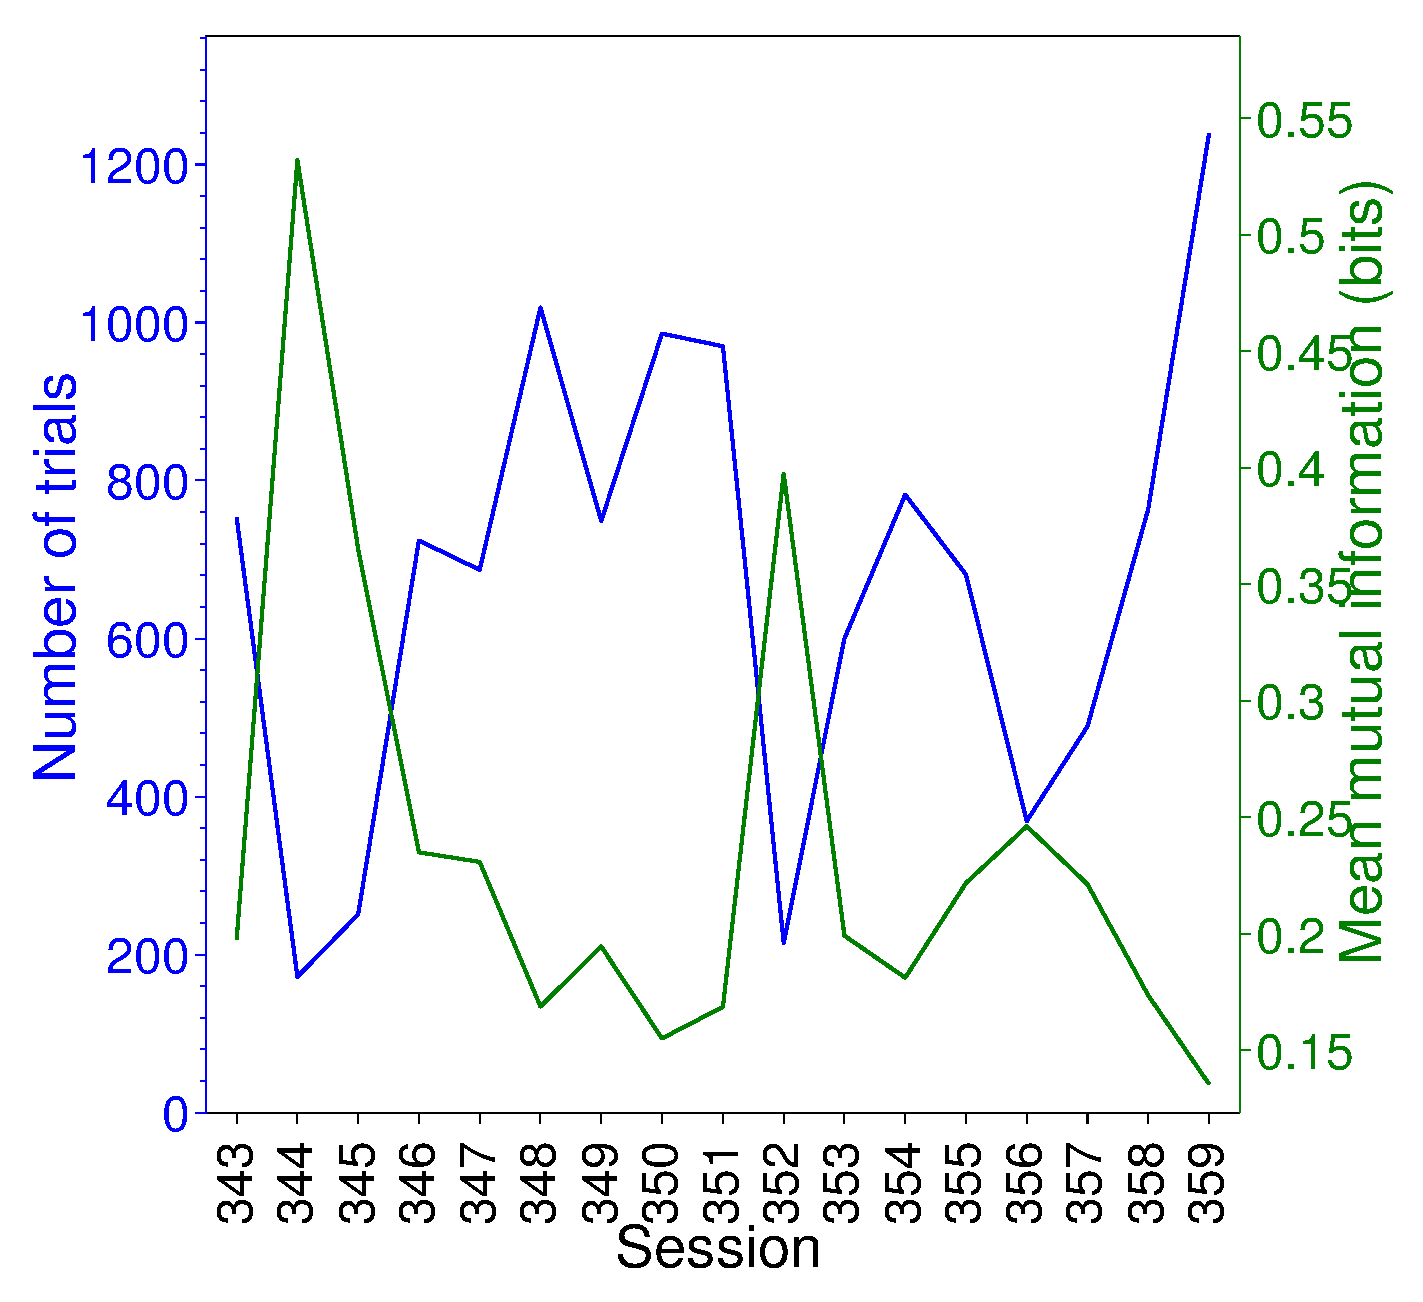
\includegraphics[width=\linewidth]{%
% % ./figs/ntrialsIandNindiv_blanco_v1_dr_naive_5bins_of_4ms_20120815T201856.eps}
% %     \end{subfigure}
% %     \begin{subfigure}[b]{0.5\linewidth}
% %         \centering
% %         \caption{M1 V4}
% %         \label{fig:IandNb4}
% %         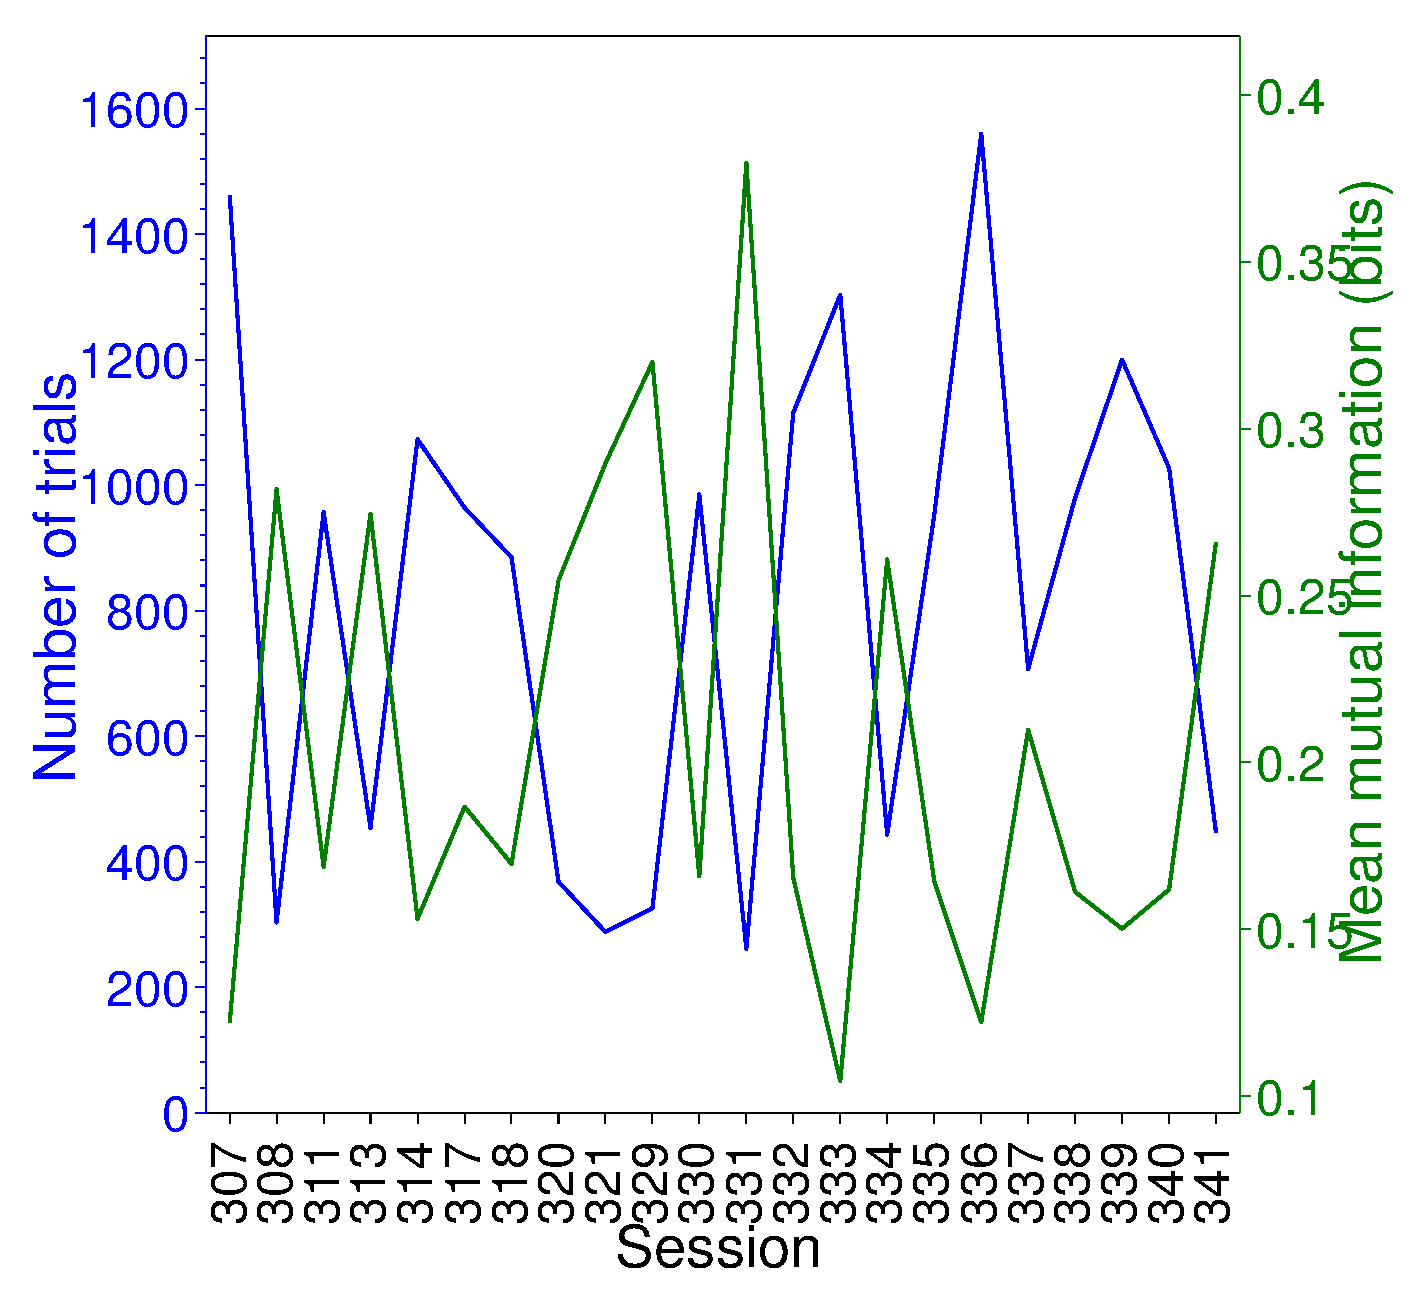
\includegraphics[width=\linewidth]{%
% % ./figs/ntrialsIandNindiv_blanco_v4_dr_naive_5bins_of_4ms_20120815T201856.eps}
% %     \end{subfigure}
% %     \\
% %     \begin{subfigure}[b]{0.5\linewidth}
% %         \centering
% %         \caption{M2 V1}
% %         \label{fig:IandNj1}
% %         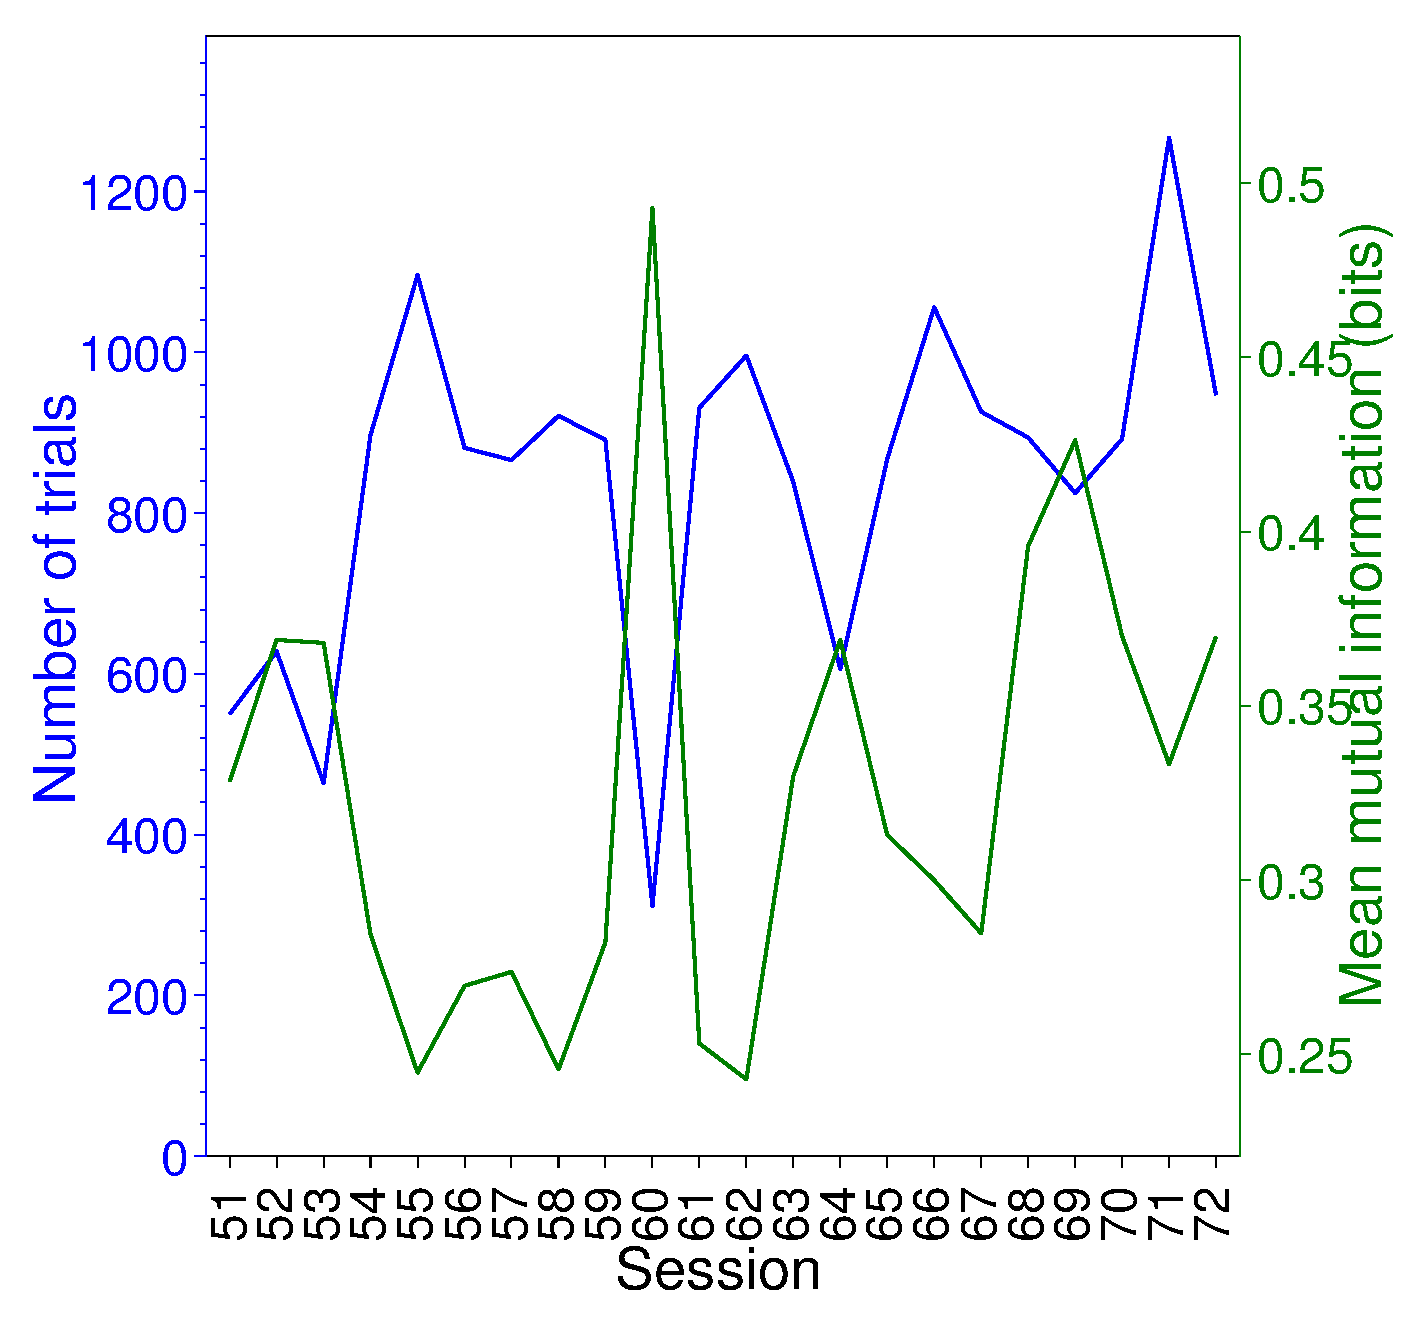
\includegraphics[width=\linewidth]{%
% % ./figs/ntrialsIandNindiv_jack_v1_dr_naive_5bins_of_4ms_20120815T201856.eps}
% %     \end{subfigure}
% %     \begin{subfigure}[b]{0.5\linewidth}
% %         \centering
% %         \caption{M2 V4}
% %         \label{fig:IandNj4}
% %         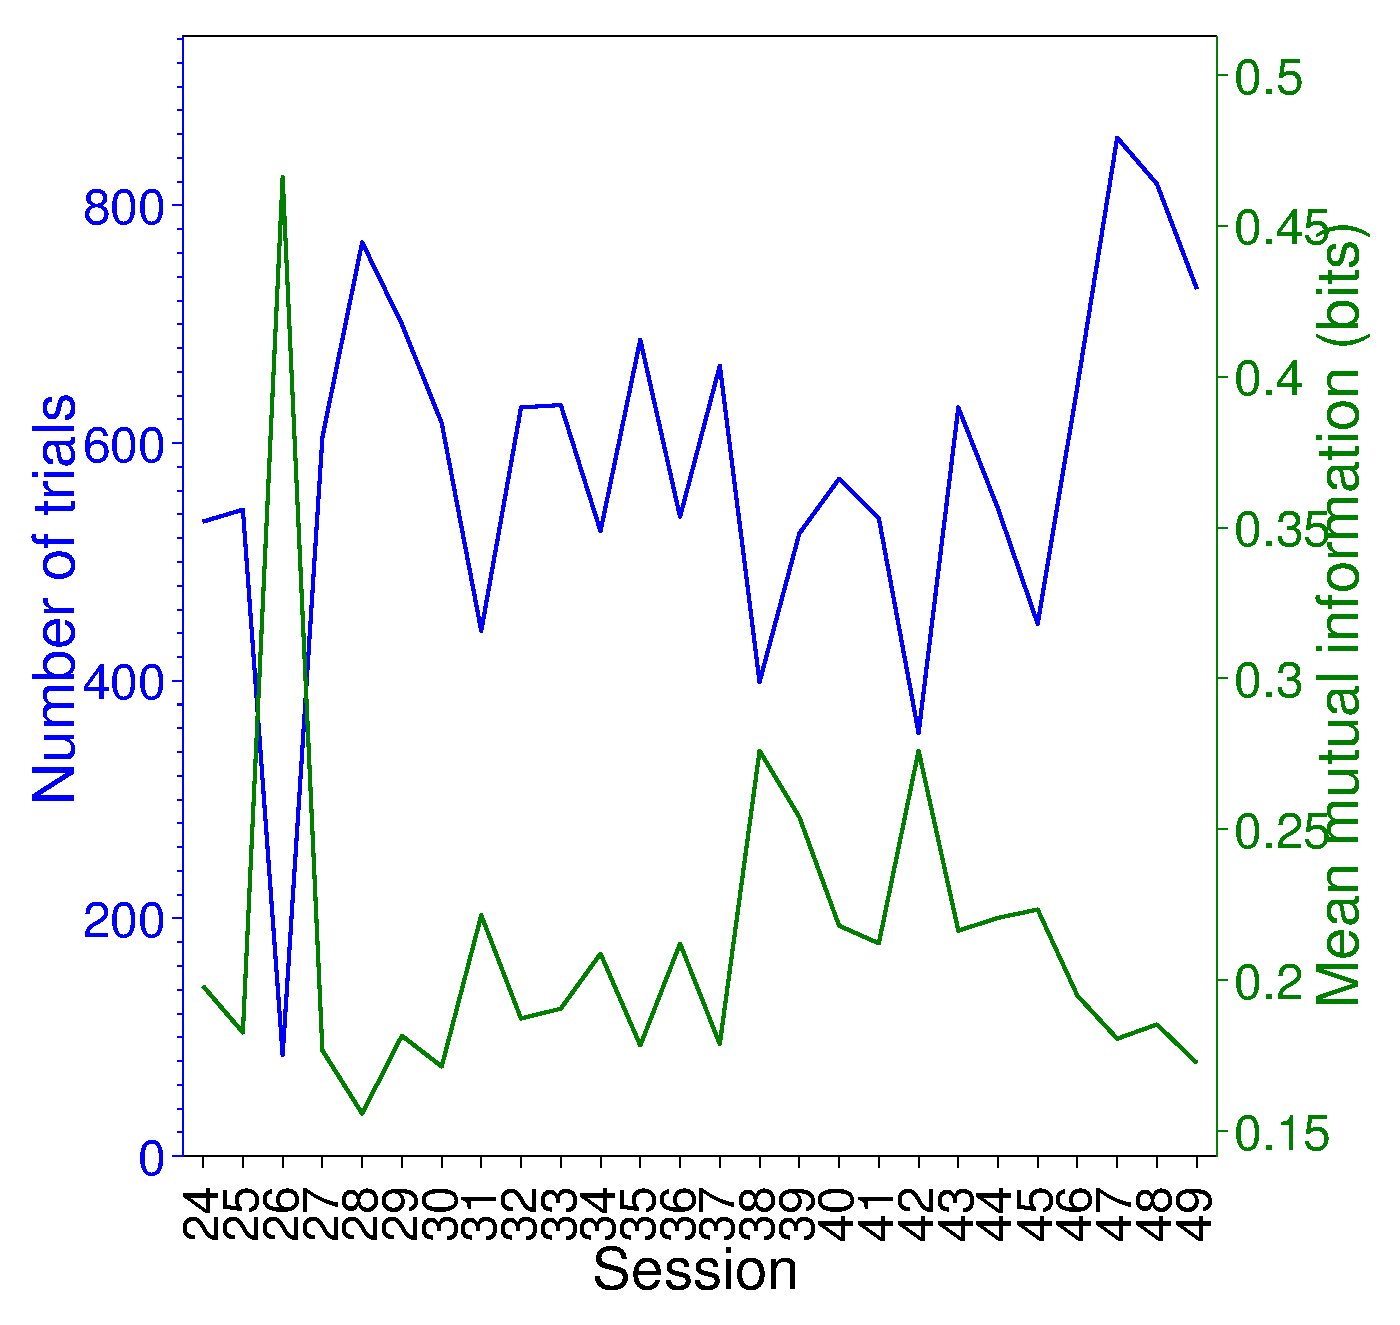
\includegraphics[width=\linewidth]{%
% % ./figs/ntrialsIandNindiv_jack_v4_dr_naive_5bins_of_4ms_20120815T201856.eps}
% %     \end{subfigure}
% %     \caption{Mutual information seems to be anti-correlated with the number of trials in the session. The number of correctly responded trials in each session is plotted on top of the mean information in individual sessions. The mutual information is the ``plug-in estimate'', not corrected for bias, and averaged across the whole period of test stimulus presentation.
% % %There is a missing data point for M2 V4 because in one session there were not enough trials per condition for the QE algorithm to function.
% % }
% %     \label{fig:IandN}
% % \end{figure}

Fig.~\ref{fig:IandN} shows that the changes in the measured mutual information are dominated by the number of trials in the session, not by increases with perceptual learning (corresponding to increments in the session number).
The only exception to this rule seems to be for M2 V1, shown in Fig.~\ref{fig:IandNj1}, where the information increases with learning despite an increase in the number of trials per session over this period.

% ./figs/ntrialsIvsinvNcombindiv_blanco_v1_20120812T164553.eps
% ./figs/ntrialsIvsinvNcombindiv_blanco_v4_20120812T164553.eps
% ./figs/ntrialsIvsinvNcombindiv_jack_v1_20120812T164553.eps
% ./figs/ntrialsIvsinvNcombindiv_jack_v4_20120812T164553.eps
% 
% ./figs/ntrialsIvsinvNcombindiv_blanco_v1_5bins_of_4ms_20120815T204808.eps
% ./figs/ntrialsIvsinvNcombindiv_blanco_v4_5bins_of_4ms_20120815T204808.eps
% ./figs/ntrialsIvsinvNcombindiv_jack_v1_5bins_of_4ms_20120815T204808.eps
% ./figs/ntrialsIvsinvNcombindiv_jack_v4_5bins_of_4ms_20120815T204808.eps
% 
% % \begin{figure}[htbp]
% %     \begin{subfigure}[b]{0.5\linewidth}
% %         \centering
% %         \caption{M1 V1}
% %         \label{fig:IvNb1}
% %         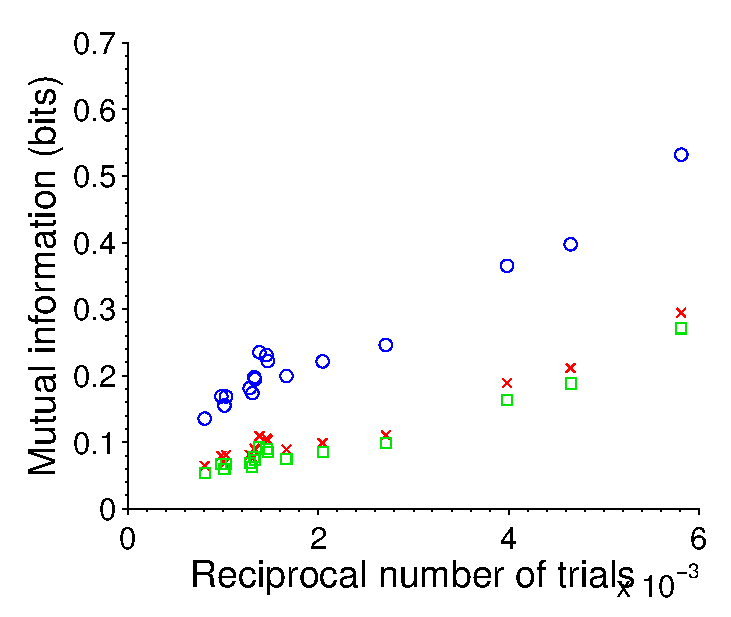
\includegraphics[width=\linewidth]{%
% % ./figs/ntrialsIvsinvNcombindiv_blanco_v1_5bins_of_4ms_20120815T204808.eps}
% %     \end{subfigure}
% %     \begin{subfigure}[b]{0.5\linewidth}
% %         \centering
% %         \caption{M1 V4}
% %         \label{fig:IvNb4}
% %         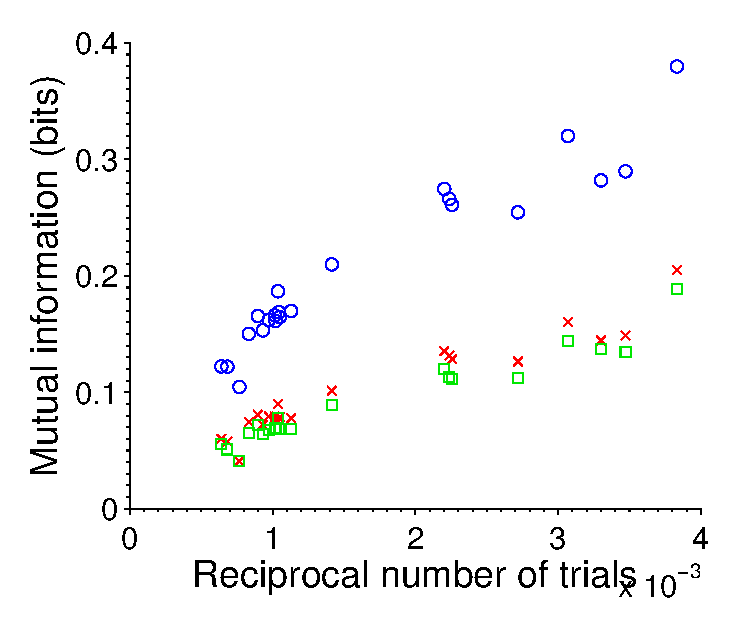
\includegraphics[width=\linewidth]{%
% % ./figs/ntrialsIvsinvNcombindiv_blanco_v4_5bins_of_4ms_20120815T204808.eps}
% %     \end{subfigure}
% %     \\
% %     \begin{subfigure}[b]{0.5\linewidth}
% %         \centering
% %         \caption{M2 V1}
% %         \label{fig:IvNj1}
% %         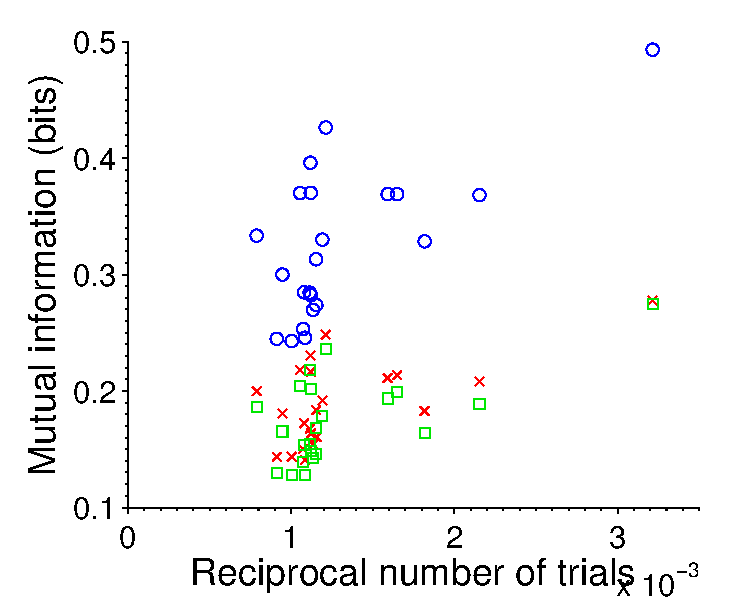
\includegraphics[width=\linewidth]{%
% % ./figs/ntrialsIvsinvNcombindiv_jack_v1_5bins_of_4ms_20120815T204808.eps}
% %     \end{subfigure}
% %     \begin{subfigure}[b]{0.5\linewidth}
% %         \centering
% %         \caption{M2 V4}
% %         \label{fig:IvNj4}
% %         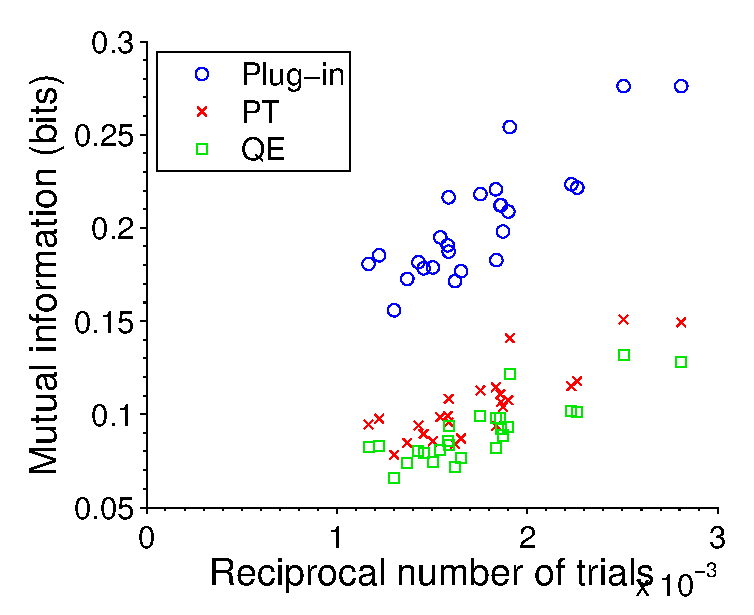
\includegraphics[width=\linewidth]{%
% % ./figs/ntrialsIvsinvNcombindiv_jack_v4_5bins_of_4ms_20120815T204808.eps}
% %     \end{subfigure}
% %     \caption{Mutual information is inversely correlated with the number of trials in the session. The mutual information for a single session is averaged over all channels, and averaged over all times during stimulus presentation, and plotted against the reciprocal of the number of trials in the session ($\nicefrac{1}{N}$). Plug-in:~with no bias correction. PT:~using the Panzeri-Treves method to correct for bias \cite{Panzeri1996}. QE:~using quadratic extrapolation for bias correction \cite{Strong1998}.
% % %There is a missing data point for M2 V4 because in one session there were not enough trials per condition for the QE algorithm to function.
% % }
% %     \label{fig:IvN}
% % \end{figure}

In particular, the measured value for the mutual information is strongly correlated with the reciprocal of the number of trials in the session (Fig.~\ref{fig:IvN}). The correlation is still very strong even if we use one of the two bias correction techniques. As discussed above, for M2 V1 the number of trials per session and the measured information  are both correlated with time, which reduces the correlation observed in Fig.~\ref{fig:IvNj1}.

The problem is that although PT and QE both do a reasonable attempt at removing the bias, they are not perfect and some bias will remain. As the bias is dependent on the number of trials, it is unsurprising the remaining bias follows the same dependency.
In particular, in the asymptotic regime the leading term in the expansion of $I_{\text{measured}}$ is known to be proportional \cite{Treves1995} to $\nicefrac{1}{N}$; the same relationship observed here.

In particular, the difficult faced is changes due to perceptual learning which are of interest may only be slight, but the the number of trials per session varies five-fold: from 250 up to 1250. Consequently it is unsurprising that the observed differences in information day-to-day are dominated by the number of trials.

% %----------------------------------------------------------------------------------------------------------------------
% \subsection{Results}
% 
% %----------------------------------------------------------------------------------------------------------------------
% \chapter{Information Theoretic Analysis (trial-wise)}
% %----------------------------------------------------------------------------------------------------------------------

%----------------------------------------------------------------------------------------------------------------------
\FloatBarrier
\subsubsection{Trial-based analysis}

To counter the correlation between measured information and number of trials, an obvious solution is to use the same number of trials for every computation. We now consider how many trials should be taken at once to obtain a reasonably reliable estimate.

Some rules-of-thumb for the number of trials are offered by \cite{Panzeri2007}.
Let $\overline{R}$ denote the number of possible response codes.
Then, for the plug-in estimate of mutual information, we need to have at least $N_S \ge 2^{32} \, \overline{R}$ trials per stimulus,
whilst if the PT or QE bias correction methods are applied, we only need $N_S > 2 \, \overline{R}$.

% The spike detection software was set to only detect spikes at least \unit[3]{ms} apart, and moreover, 
The probability of having two spikes within \unit[4]{ms} from a non-bursting neuron is very low. For example, a neuron with a high firing rate might fire at \unit[100]{Hz}, which means inter-spike intervals are typically around \unit[10]{ms} (and \unit[100]{Hz} is a high firing rate for the channels in our dataset).
Consequently any \unit[4]{ms} bin will realistically contain either 0 or 1 spikes, and the number of possible response codes in our spike timing code analysis with 5 bins each of \unit[4]{ms} is $\overline{R} = 2^5 = 32$. In comparison for a spike count code, if we assume spikes cannot be closer together than \unit[3]{ms}, there are between 0 and 7 spikes in any \unit[20]{ms} interval. Consequently there are $\overline{R} = 8$ possible response codes.

As we wish our analysis to work for both spike timing and spike count codes, using the above rules we need to use at least 64 trials per stimulus to get a reasonable estimate of the information with one of the bias correction methods in place.
Since there are 14 different stimuli, this means at least 896 trials in total are needed. This presents a dilemma, since most of the sessions are shorter than this, even when both correctly and incorrectly responded trials are included. Excluding sessions with fewer than 896 trials would severely limit the size of the dataset.
% and the patchwork of holes which would result would limit how much can be read into the results due to  which would result.

The solution found was to concatenate the sessions together and analyse groups of $N$ trials taken from multiple consecutive sessions.
The na\"{i}ve justification for this approach is a ``first-order approximation'' to perceptual learning would be that the monkey gets better at recognising the stimuli every-time they perceive it, and so the most important quantifier for the amount of perceptual learning which has taken place is the total number of trials the monkey has performed to date.

This rather basic assumption neglects several factors which influence the animal's performance, such as their mood during the particular training day; and factors which influence the animal's willingness to work (in turn influencing performance), which depends on their recent level of access to water (the reward used in the study). For instance, the animal performs less well on Mondays, which follows on from readily available water during the weekend.
Furthermore, the consolidation which occurs during sleep is commonly believed to be important to perceptual learning, and (as this only occurs between training sessions) this effect is completely ignored by this approach.

However, the session-concatenation approach was attempted regardless, and a value of $N_S = 100$ trials per stimulus was chosen. Though there are enough trials available to use more and reduce the bias further, it is undesirable data from so many sessions at once.

As mentioned in Chap.~\ref{ch:exp}, a delayed repeat is used for any trials to which the animal does not correctly respond. Consequently, more difficult test stimuli (with contrasts close to the sample contrast) are presented significantly more frequently than easier stimuli.
For instance, when presented with the most difficult test stimuli, the animal will have a success rate only just above 50\% on the first day of the experiment, rising to around 70\% by the last day. For the easiest stimuli, the success rate will be nearly 100\% throughout.

Say we arrange all the trials into groups based on their stimulus, then take 100 subsequent trials from each of the groups to perform the analysis on. Due to the different number of trials per stimulus, it will not be long before the trials selected for each stimulus are from very different points in time and from different sessions.\footnote{Even if we only analyse the correctly responded trials, there is still a difference in the number of trials per stimulus due to a limit on the number of repeats of any test condition. The difference was negligible for M1, but accumulated to a 100 trial difference over all the sessions between the most and least correctly responded conditions for M2.}
To ensure all the trials are from when the animal has had the same amount of training, we can instead take a group of $S \cdot N_S = 14 \cdot 100 = 1400$ consecutive trials regardless of the stimulus presented and analysed. The differences in number of trials per stimulus are not particularly important, so long as there are always  enough.

All trials where the monkey completed the trial and gave a response (either correct or incorrect) were included in the analysis. Trials where the monkey did not complete the task by fixating and then providing a response as required were excluded.
Using both the correct and incorrectly responded trials means our distribution for $P(s)$ is the same as that presented to the monkey, and there are notably more trials available to perform the analysis on.

% Using 50 and 100 trials explored: not considerable difference between results. 100 shown for conciseness

%----------------------------------------------------------------------------------------------------------------------
\FloatBarrier
\subsubsection{Information in fine vs. coarse distinctions}

The difference between information about fine differences in contrast can be studied by only considering trials where the contrast presented is one of the middle 6 contrasts:
\{22, 25, 28, 32, 35, 40\}\% for V1 and
\{27, 28, 29, 31, 32, 33\}\% for V4.
To keep the dimensionality of the stimulus the same, this has been compared to the information across some more separated contrasts:
 \{5, 15, 22, 40, 50, 90\}\% for V1 and
\{10, 15, 20, 40, 50, 60\}\% for V4.
For V4, the group of coarsely differentiated contrasts is the outer most six contrasts, but for V1 the coarsely differentiated contrasts are alternate

%----------------------------------------------------------------------------------------------------------------------
\FloatBarrier
\subsubsection{Information in spike timing code vs. spike count code}

Because the possible responses in the spike timing and count codes have different dimensionality, they have different biases \cite{Panzeri2007} and it is not possible to compare them directly.
Consequently, to investigate how much more information there is in a spike timing based code we must consider a set of responses which have the same dimensionality, but lack the timing information.

To do this, the spike-timing response codes are taken, then shuffled across the 5 bins for every individual trial.%
\footnote{The shuffling of bins was performed using the open source Shuffle.m
available from \url{http://www.mathworks.com/matlabcentral/fileexchange/27076-shuffle}.}
Since the 5 bins are now in a random order, any information contained in their order is lost. To make ensure the estimate of the information in the spike-timing code with the timing information destroyed was reasonable, the information was measured for five different shuffles%
% \footnote{The five shuffles were performed with a random seed linked to microsecond of execution time.}
 and then the mean was taken.

The information contained in the \unit[4]{ms} level spike timing can then be found by subtracting the mean shuffled information from the unshuffled information.

%----------------------------------------------------------------------------------------------------------------------
\FloatBarrier
\subsubsection{Spontaneous activity}

To check whether changes in the data quality between sessions and other differences between sessions could be influencing the results, the information theoretic analysis was also applied the spontaneous activity from the animal.
In particular, the spontaneous activity from prior to the sample presentation was used, so the animal had not yet seen the test contrast.
Although monkey's brain activity cannot possibly contain any genuine information about the test contrast, we expect to measure a non-zero value for the information content due to the sampling bias.

%----------------------------------------------------------------------------------------------------------------------
%----------------------------------------------------------------------------------------------------------------------
%----------------------------------------------------------------------------------------------------------------------
\subsection{Results}

During the course of the analysis, results were inspected using PT and using QE for bias correction. The plots were similar in distribution, and each gave a similar magnitude for the information. However, PT gave visibly lower variance than QE, so only plots using PT are presented in this results section.
Using the $I_{\text{sh}}$ approach where the bias is corrected by shuffling bins across trials \cite{Montemurro2007} was also attempted for the spike timing code, but this increased the variance far too much to be of any practical use. The unexpectedly significant increase in variance is probably due to the nature of the correlations between the bins which are being shuffled.

We also compared some of the results both with the monitor artifact left in the data and with the dataset redacted to have it removed. There was no appreciable difference for any of the plots, though the amount of information went down when the data was redacted due to the loss of some of the spikes.

%----------------------------------------------------------------------------------------------------------------------
% \FloatBarrier
% \subsubsection{General Information plots}

Starting with V1, the first thing which is noticed in Figs.~\ref{fig:b1-trialwise} and \ref{fig:j1-trialwise} \ref{fig:b1-1x20tp4} and \ref{fig:b1-5x4tp4} is the large peak in information over the \unit[20]{ms} window starting at around \unit[40]{ms} after stimulus onset. This is due to the onset transient response, where there is a larger amount of neural activity, and this is also less variable than usual \cite{Muller2001}. A second, smaller peak from the ``rebound'' of the transient also occurs around \unit[100]{ms} after stimulus onset. Looking at the scalebars, we can see there is about 10 times as much information on average from the neurons in M2 than M1. This is probably due to differences in data quality between the two animals.

Comparing the information found using the spike timing code \ref{fig:b1-5x4tp4} with the spike count code \ref{fig:b1-1x20tp4}, it seems that there is significantly more information when the binned spike times are considered: there is three times as much information for the spike timing code for M1 and twice as much for M2. However, if we look at information in the spontaneous activity, this reveals we cannot trust this result, as the bias for the information from the spontaneous activity is much higher for the spike timing code than spike count.

For M1, aside from the transient, the information measured with the spike timing code from the spontaneous activity is about the same as the information from the test presentation, suggesting something has gone very wrong!

For the spike timing codes, there is a clear decrease in information with learning in M1, and a clear increase in information for M2. This is, however, present in both the test presentation activity and the spontaneous activity, suggesting it is not a genuine effect. This is believed to be due to a decrease in signal quality in the implants in M1, and possibly an increase in M2.
The increase is also seen in the spike count code for M2, but not to any real extent and it is doubtful that the result is significant.

The bias in the information for the spontaneous activity changes with time for the spike timing code, but does not for the spike count code.
Since any changes in the dataset are the same for both of these, this suggests there are too few trials for the spike timing code to give a reliable reading of the information. This would make sense because with an average of $N_S = 100$ trials per stimulus and a spike timing code with $\overline{R} = 32$, there are
on average $\nicefrac{N_S}{\overline{R}} = 3.125$ trials per response per stimulus,
whilst for a spike count code with $\overline{R} = 8$ there are on average $\nicefrac{N_S}{\overline{R}} = 12.5$ trials per response per stimulus.
Similarly if there we assume a minimum of $N_S = 64$ trials per stimulus, there are
at least $\nicefrac{N_S}{\overline{R}} > 2$ trials per response per stimulus for the spike timing code, and
at least $\nicefrac{N_S}{\overline{R}} > 8$ trials per response per stimulus for the spike count code.

The information in the spontaneous activity was subsequently computed with an average of $N_S = 200$ and with $N_S = 400$ trials per stimulus.
This means there is now $\nicefrac{N_S}{\overline{R}} > 8$ for the spike timing code, however precisely the same relationship was observed.
From this, we can conclude the problem is due to the inconsistencies between sessions. If the firing rate changes between two sessions, the probability distribution of the responses generated will change for each condition. This will not matter so much for the spike count code because there are only 8 possible responses, and even if there are only 250 trials in the session there should be at least 16 trials per condition, meeting the minimal requirements for the PT method to function.

The small bump in the information in the spontaneous activity around \unit[50]{ms} in Figs.~\ref{fig:b1-5x4tp4} and \ref{fig:j1-5x4tp4} will be due to an increase in activity from a transient response. This data is normalised so \unit[0]{ms} is when the animal begins fixating on the fixation target, and there will be a transient response after the animal saccades to the target. Although the increase in activity does not relate to the conditions used on the subsequent test presentation, the extra spikes will increase the variability of the response, and thus $H(\SET{R})$, which will not be cancelled out by an increase in $H(\SET{R}|\SET{S})$ for the same reasons the bias appears in the first place.

In short, the data for M1 V1 does not seem to be of good enough quality whilst M2 V1 does, and the information in the spike timing code cannot be trusted for either monkey.

%  ./figs/I_trialwise_blanco_v1_chmean23_s343-354,355.1,355.2,356-359_tp4_1bins_of_20ms_dr_pt_oc0_test_tc5-5-20,22-3-28,32,35-5-50,60,90_nt1400_ts350_rmvet1_rmvms0_pcolorhot_20120815T234452.png
% ./figs/I_trialwise_blanco_v1_chmean23_s343-354,355.1,355.2,356-359_tp1_1bins_of_20ms_dr_pt_oc0_test_tc5-5-20,22-3-28,32,35-5-50,60,90_nt1400_ts350_rmvet1_rmvms0_pcolorhot_20120815T234326.png
% ./figs/I_trialwise_blanco_v1_chmean23_s343-354,355.1,355.2,356-359_tp4_1bins_of_20ms_dr_pt_oc0_test_tc5-5-20,22-3-28,32,35-5-50,60,90_nt1400_ts350_rmvet1_rmvms1_pcolorhot_20120815T234741.png
% ./figs/I_trialwise_blanco_v1_chmean23_s343-354,355.1,355.2,356-359_tp1_1bins_of_20ms_dr_pt_oc0_test_tc5-5-20,22-3-28,32,35-5-50,60,90_nt1400_ts350_rmvet1_rmvms1_pcolorbp_20120816T175451.png
% ./figs/I_trialwise_blanco_v1_chmean23_s343-354,355.1,355.2,356-359_tp4_5bins_of_4ms_dr_pt_oc0_test_tc5-5-20,22-3-28,32,35-5-50,60,90_nt1400_ts350_rmvet1_rmvms1_pcolorhot_20120815T234513.png
% ./figs/I_trialwise_blanco_v1_chmean23_s343-354,355.1,355.2,356-359_tp1_5bins_of_4ms_dr_pt_oc0_test_tc5-5-20,22-3-28,32,35-5-50,60,90_nt1400_ts350_rmvet1_rmvms1_pcolorbp_20120816T175423.png

% % \cleartoevenpage

% % \begin{figure}[htbp]
% % %     \begin{subfigure}[b]{0.5\linewidth}
% % %         \centering
% % %         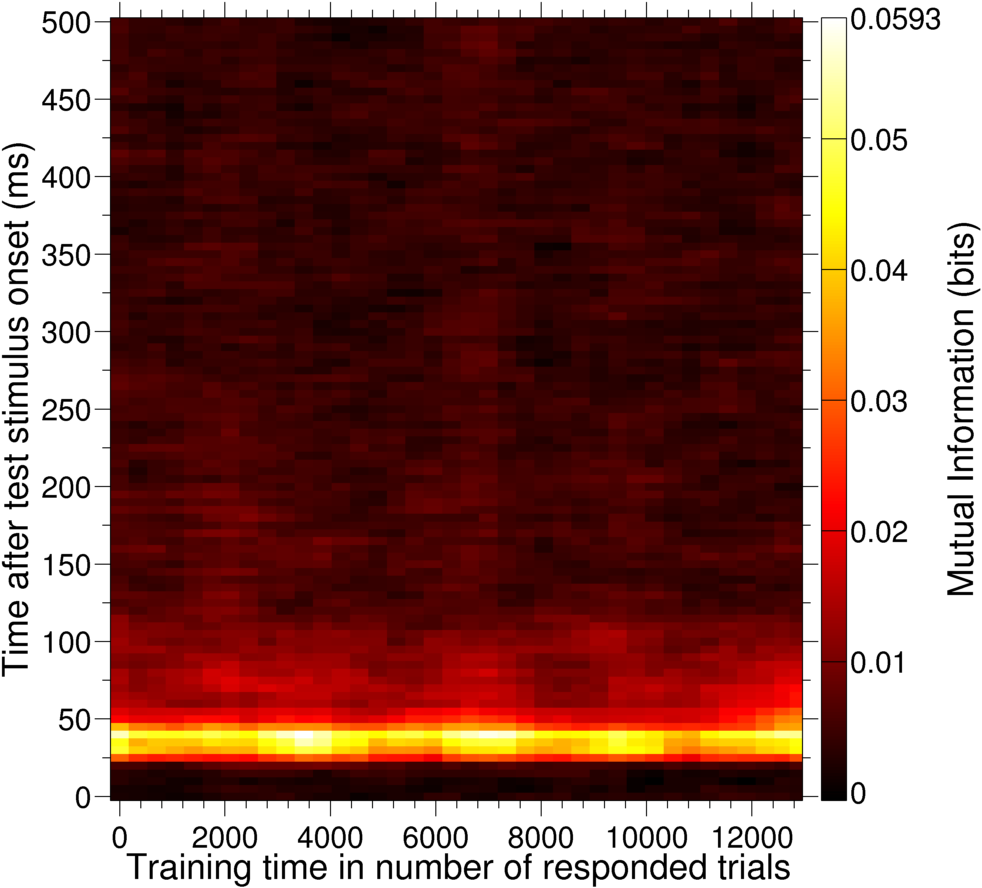
\includegraphics[scale=.25]{%
% % % ./figs/I_trialwise_blanco_v1_chmean23_s343-354,355.1,355.2,356-359_tp4_1bins_of_20ms_dr_pt_oc0_test_tc5-5-20,22-3-28,32,35-5-50,60,90_nt1400_ts350_rmvet1_rmvms0_pcolorhot_20120815T234452.png}
% % %         \caption{}
% % %         \label{fig:b1-1x20tp4ma}
% % %     \end{subfigure}
% % %     ~~
% % %     \begin{subfigure}[b]{0.5\linewidth}
% % %         \centering
% % %         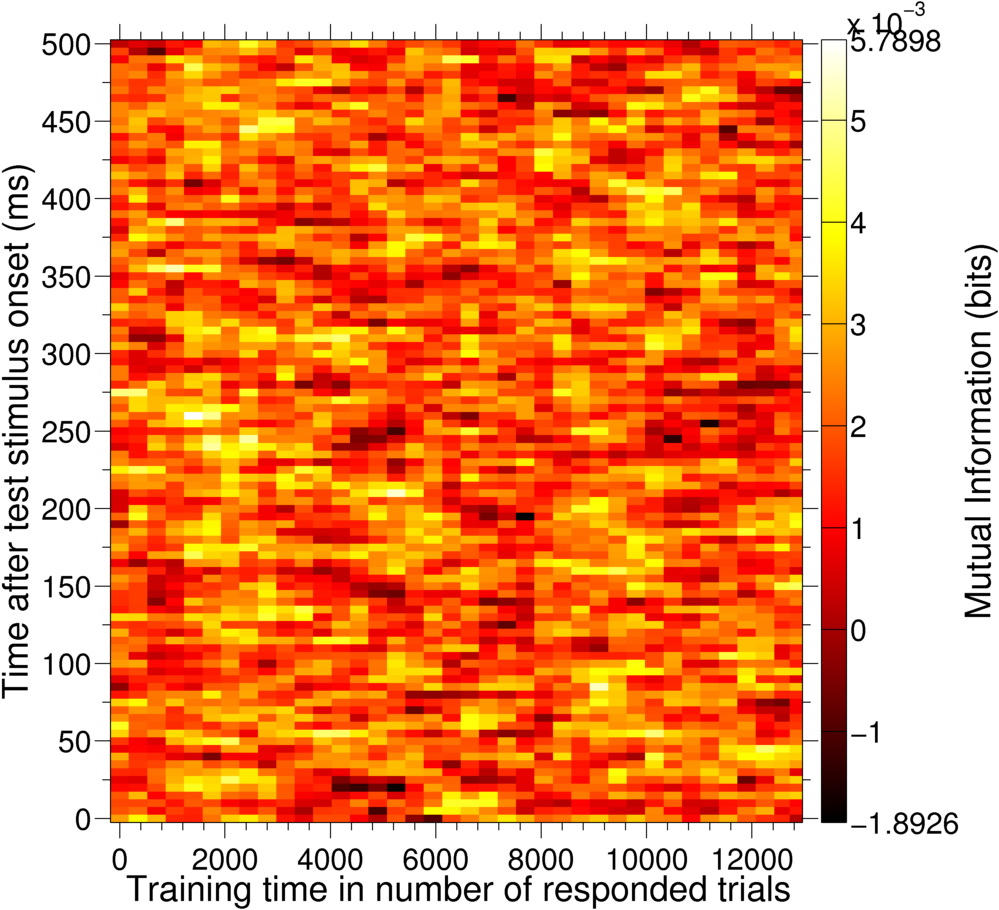
\includegraphics[scale=.25]{%
% % % ./figs/I_trialwise_blanco_v1_chmean23_s343-354,355.1,355.2,356-359_tp1_1bins_of_20ms_dr_pt_oc0_test_tc5-5-20,22-3-28,32,35-5-50,60,90_nt1400_ts350_rmvet1_rmvms0_pcolorhot_20120815T234326.png}
% % %         \caption{}
% % %         \label{fig:b1-1x20tp1ma}
% % %     \end{subfigure}
% % %     \\
% %     \begin{subfigure}[b]{0.5\linewidth}
% %         \centering
% %         \caption{}
% %         \label{fig:b1-1x20tp4}
% %         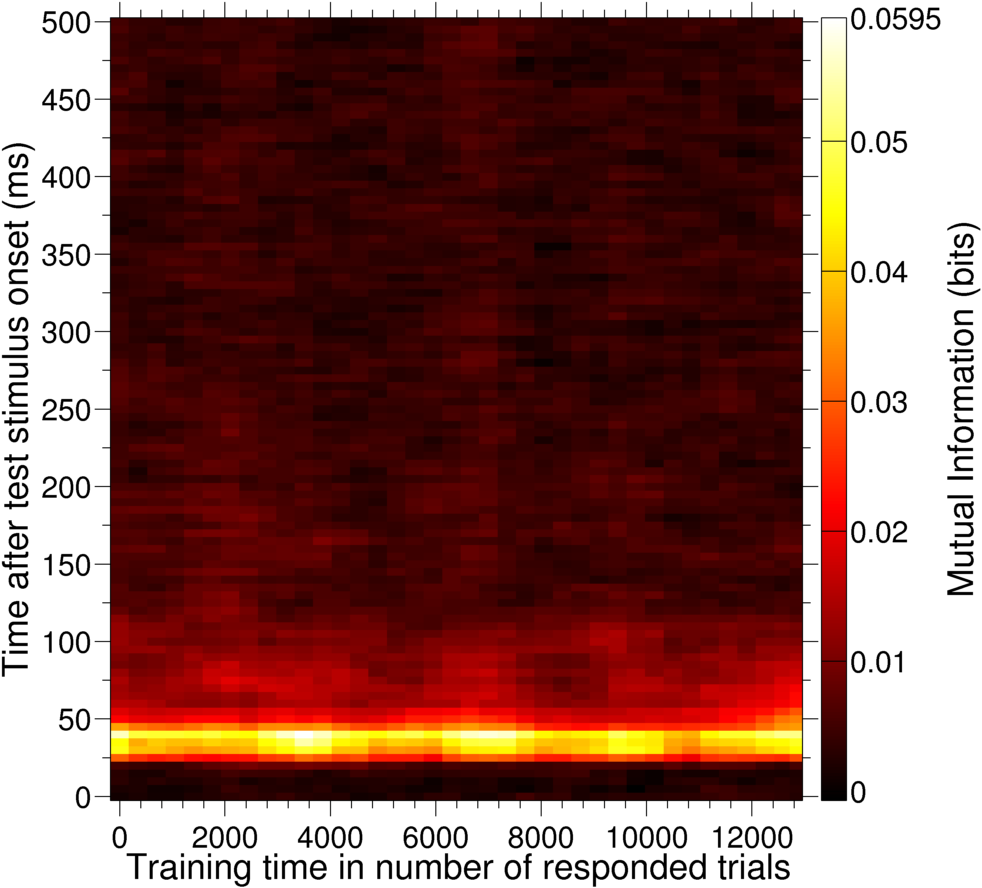
\includegraphics[scale=.25]{%
% % ./figs/I_trialwise_blanco_v1_chmean23_s343-354,355.1,355.2,356-359_tp4_1bins_of_20ms_dr_pt_oc0_test_tc5-5-20,22-3-28,32,35-5-50,60,90_nt1400_ts350_rmvet1_rmvms1_pcolorhot_20120815T234741.png}
% %     \end{subfigure}
% %     ~~
% %     \begin{subfigure}[b]{0.5\linewidth}
% %         \centering
% %         \caption{}
% %         \label{fig:b1-1x20tp1}
% %         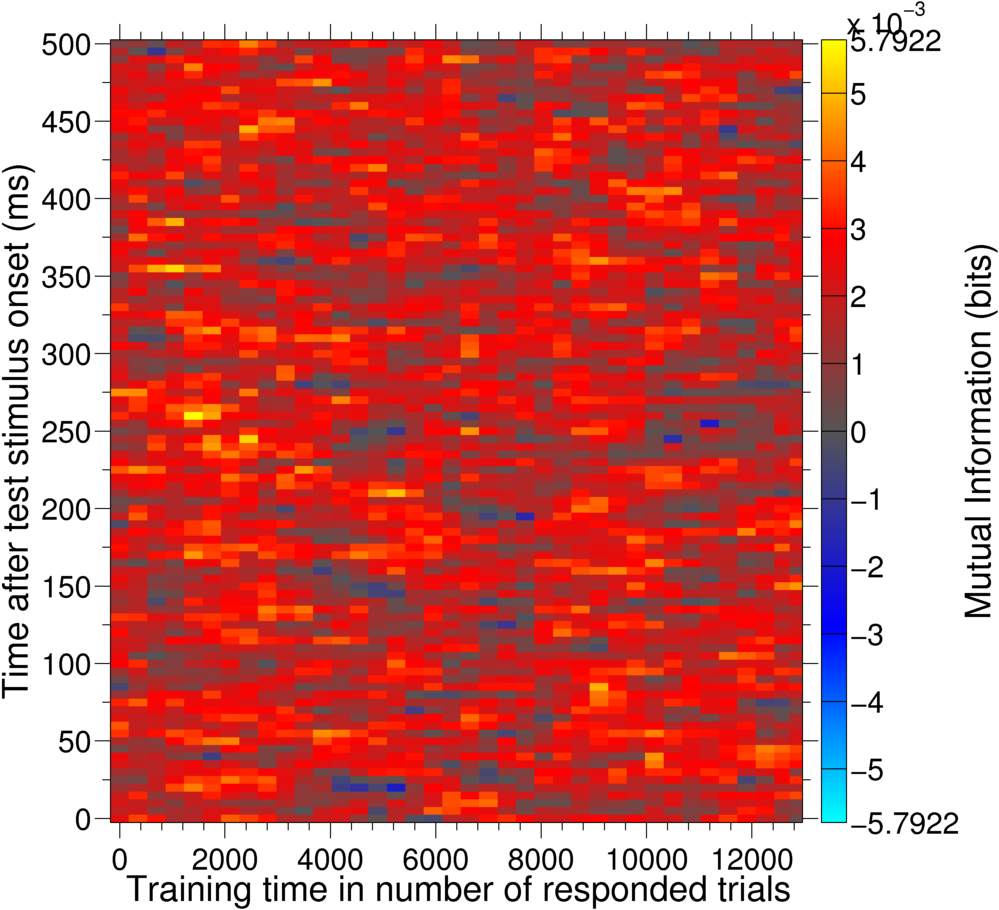
\includegraphics[scale=.25]{%
% % ./figs/I_trialwise_blanco_v1_chmean23_s343-354,355.1,355.2,356-359_tp1_1bins_of_20ms_dr_pt_oc0_test_tc5-5-20,22-3-28,32,35-5-50,60,90_nt1400_ts350_rmvet1_rmvms1_pcolorbp_20120816T175451.png}
% %     \end{subfigure}
% %     \\
% %     \begin{subfigure}[b]{0.5\linewidth}
% %         \centering
% %         \caption{}
% %         \label{fig:b1-5x4tp4}
% %         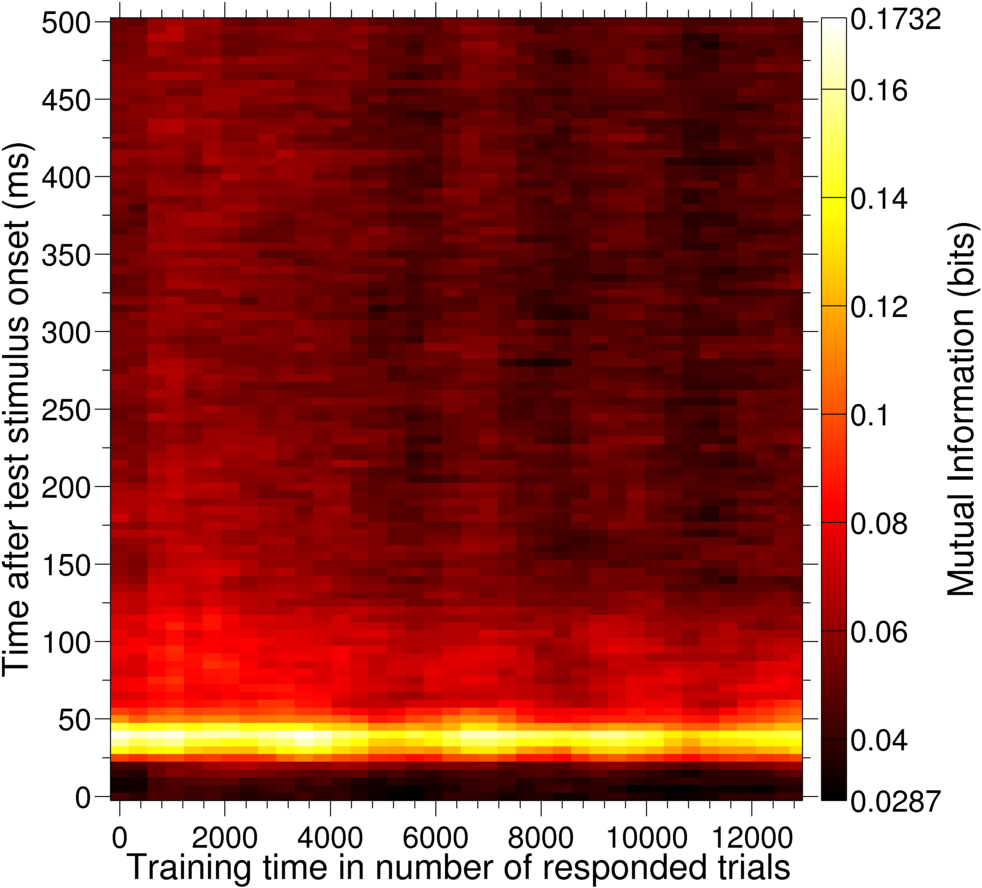
\includegraphics[scale=.25]{%
% % ./figs/I_trialwise_blanco_v1_chmean23_s343-354,355.1,355.2,356-359_tp4_5bins_of_4ms_dr_pt_oc0_test_tc5-5-20,22-3-28,32,35-5-50,60,90_nt1400_ts350_rmvet1_rmvms1_pcolorhot_20120815T234513.png}
% %     \end{subfigure}
% %     ~~
% %     \begin{subfigure}[b]{0.5\linewidth}
% %         \centering
% %         \caption{}
% %         \label{fig:b1-5x4tp1}
% %         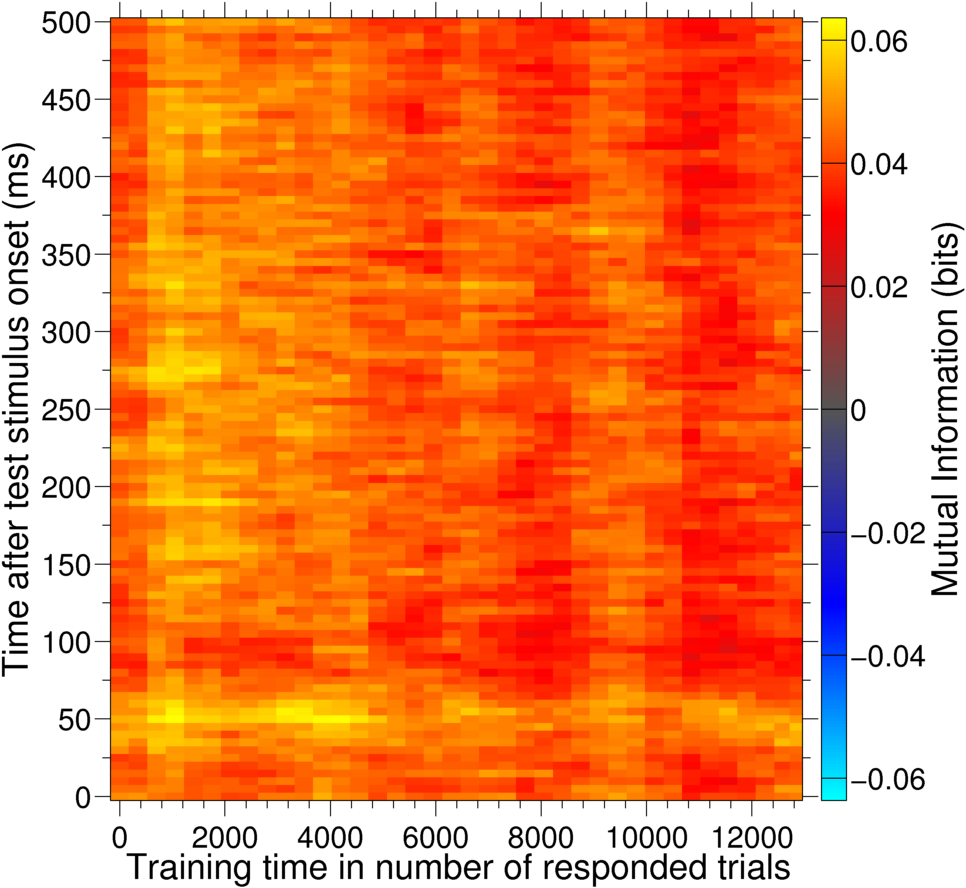
\includegraphics[scale=.25]{%
% % ./figs/I_trialwise_blanco_v1_chmean23_s343-354,355.1,355.2,356-359_tp1_5bins_of_4ms_dr_pt_oc0_test_tc5-5-20,22-3-28,32,35-5-50,60,90_nt1400_ts350_rmvet1_rmvms1_pcolorbp_20120816T175423.png}
% %     \end{subfigure}
% %     \caption{M1 V1: Mutual information between the test stimulus and \unit[20]{ms} of spiking activity, averaged across 23 channels.
% % The PT bias correction method was used in all estimates of the information, and the modification to the spiking data to remove the artifact as described in Sec.~\ref{sec:ma} was performed.
% % The neural code used in \ref{fig:b1-1x20tp4}, \ref{fig:b1-1x20tp1} is a spike count code, whilst in \ref{fig:b1-5x4tp4} and \ref{fig:b1-5x4tp1} it is a spike timing code where the \unit[20]{ms} window was subdivided into 5 bins each of \unit[4]{ms}.
% % In \ref{fig:b1-1x20tp4} and \ref{fig:b1-5x4tp4} the spike-train is taken from the test presentation part of the trial;
% % for \ref{fig:b1-1x20tp1} and \ref{fig:b1-5x4tp1} the spike-train is taken from spontaneous pre-stimulus activity.
% % The data is sampled in intervals of \unit[350]{trials} in the $x$-direction and \unit[5]{ms} in the $y$-direction, so there is significant correlation between any pair of pixels in the image with less than 4 pixels between them in either cartesian direction.
% % % In \ref{fig:b1-1x20tp4ma}, \ref{fig:b1-1x20tp4}, and \ref{fig:b1-5x4tp4}, the spike-train is taken from the test presentation part of the trial;
% % % for \ref{fig:b1-1x20tp1ma}, \ref{fig:b1-1x20tp1}, and \ref{fig:b1-5x4tp1}, the spike-train is taken from spontaneous pre-stimulus activity.
% % % In \ref{fig:b1-1x20tp4ma} and \ref{fig:b1-1x20tp1ma} no attempt was made to remove the monitor artifact from the raw data, whilst in the rest of the panels the data was modified to counter this as described in \ref{sec:ma}.
% % % \ref{fig:b1-1x20tp4ma}
% % % \ref{fig:b1-1x20tp1ma}
% % % \ref{fig:b1-1x20tp4}
% % % \ref{fig:b1-1x20tp1}
% % % \ref{fig:b1-5x4tp4}
% % % \ref{fig:b1-5x4tp1}
% % }
% %     \label{fig:b1-trialwise}
% % \end{figure}


% ./figs/I_trialwise_jack_v1_chmean25_s51-72_tp4_1bins_of_20ms_dr_pt_oc0_test_tc5-5-20,22-3-28,32,35-5-50,60,90_nt1400_ts350_rmvet1_rmvms0_pcolorhot_20120815T234410.png
% ./figs/I_trialwise_jack_v1_chmean25_s51-72_tp1_1bins_of_20ms_dr_pt_oc0_test_tc5-5-20,22-3-28,32,35-5-50,60,90_nt1400_ts350_rmvet1_rmvms0_pcolorhot_20120815T234245.png
% ./figs/I_trialwise_jack_v1_chmean25_s51-72_tp4_1bins_of_20ms_dr_pt_oc0_test_tc5-5-20,22-3-28,32,35-5-50,60,90_nt1400_ts350_rmvet1_rmvms1_pcolorhot_20120815T234701.png
% ./figs/I_trialwise_jack_v1_chmean25_s51-72_tp1_1bins_of_20ms_dr_pt_oc0_test_tc5-5-20,22-3-28,32,35-5-50,60,90_nt1400_ts350_rmvet1_rmvms1_pcolorbp_20120816T175411.png
% ./figs/I_trialwise_jack_v1_chmean25_s51-72_tp4_5bins_of_4ms_dr_pt_oc0_test_tc5-5-20,22-3-28,32,35-5-50,60,90_nt1400_ts350_rmvet1_rmvms1_pcolorhot_20120815T234434.png
% ./figs/I_trialwise_jack_v1_chmean25_s51-72_tp1_5bins_of_4ms_dr_pt_oc0_test_tc5-5-20,22-3-28,32,35-5-50,60,90_nt1400_ts350_rmvet1_rmvms1_pcolorbp_20120816T175343.png

% % \begin{figure}[htbp]
% % %     \begin{subfigure}[b]{0.5\linewidth}
% % %         \centering
% % %         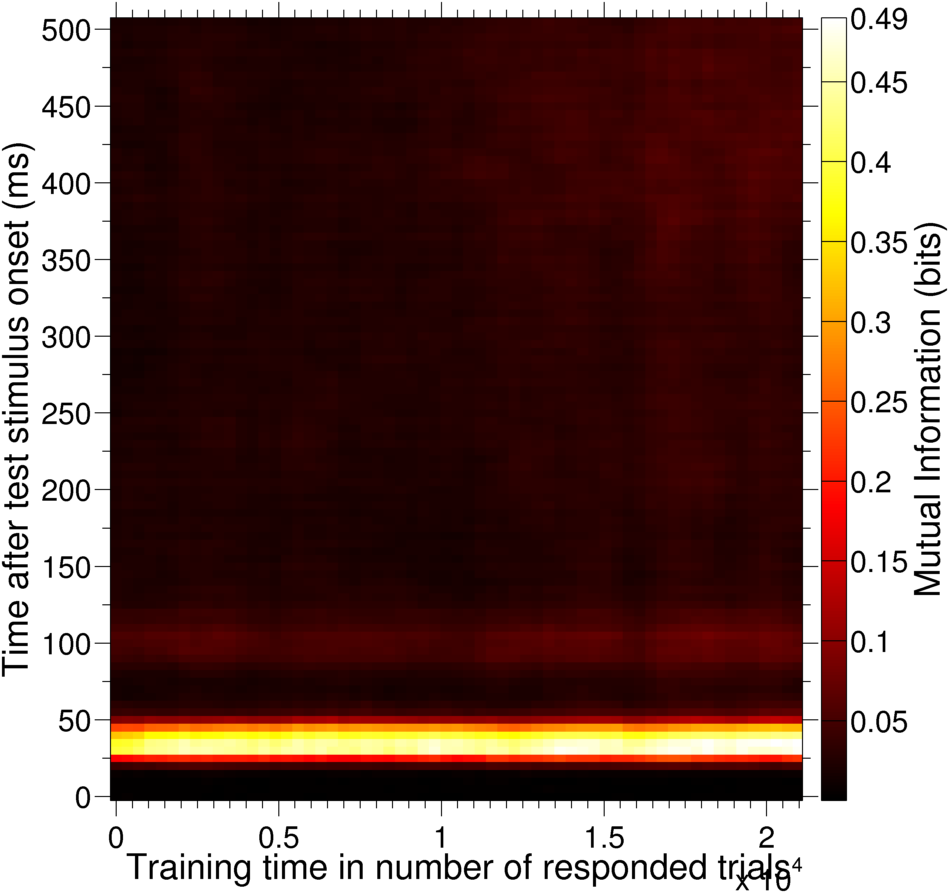
\includegraphics[scale=.25]{%
% % % ./figs/I_trialwise_jack_v1_chmean25_s51-72_tp4_1bins_of_20ms_dr_pt_oc0_test_tc5-5-20,22-3-28,32,35-5-50,60,90_nt1400_ts350_rmvet1_rmvms0_pcolorhot_20120815T234410.png}
% % %         \caption{}
% % %         \label{fig:j1-1x20tp4ma}
% % %     \end{subfigure}
% % %     ~~
% % %     \begin{subfigure}[b]{0.5\linewidth}
% % %         \centering
% % %         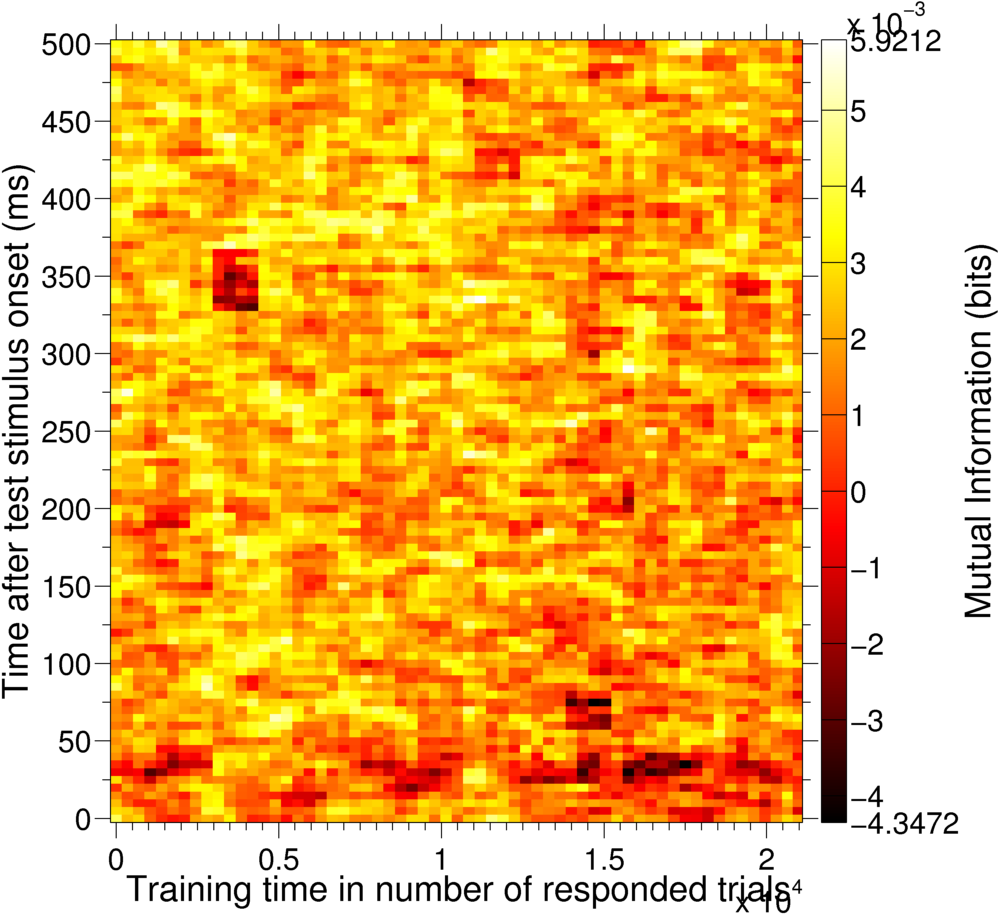
\includegraphics[scale=.25]{%
% % % ./figs/I_trialwise_jack_v1_chmean25_s51-72_tp1_1bins_of_20ms_dr_pt_oc0_test_tc5-5-20,22-3-28,32,35-5-50,60,90_nt1400_ts350_rmvet1_rmvms0_pcolorhot_20120815T234245.png}
% % %         \caption{}
% % %         \label{fig:j1-1x20tp1ma}
% % %     \end{subfigure}
% % %     \\
% %     \begin{subfigure}[b]{0.5\linewidth}
% %         \centering
% %         \caption{}
% %         \label{fig:j1-1x20tp4}
% %         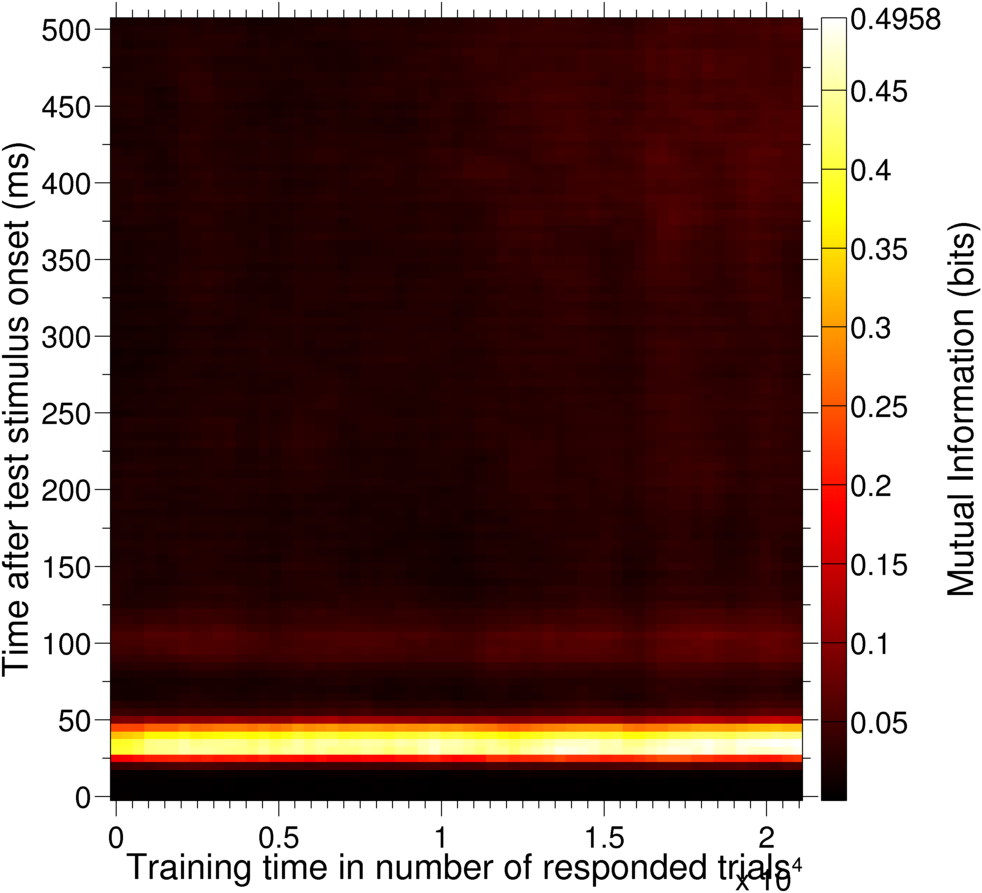
\includegraphics[scale=.25]{%
% % ./figs/I_trialwise_jack_v1_chmean25_s51-72_tp4_1bins_of_20ms_dr_pt_oc0_test_tc5-5-20,22-3-28,32,35-5-50,60,90_nt1400_ts350_rmvet1_rmvms1_pcolorhot_20120815T234701.png}
% %     \end{subfigure}
% %     ~~
% %     \begin{subfigure}[b]{0.5\linewidth}
% %         \centering
% %         \caption{}
% %         \label{fig:j1-1x20tp1}
% %         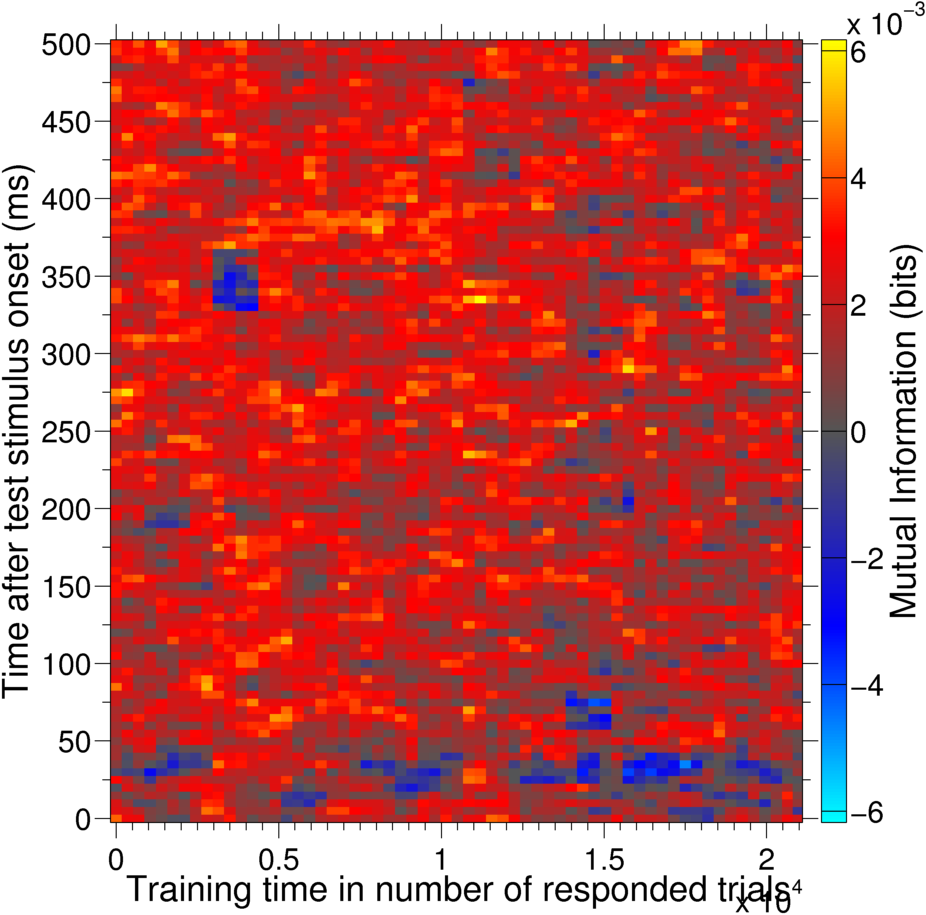
\includegraphics[scale=.25]{%
% % ./figs/I_trialwise_jack_v1_chmean25_s51-72_tp1_1bins_of_20ms_dr_pt_oc0_test_tc5-5-20,22-3-28,32,35-5-50,60,90_nt1400_ts350_rmvet1_rmvms1_pcolorbp_20120816T175411.png}
% %     \end{subfigure}
% %     \\
% %     \begin{subfigure}[b]{0.5\linewidth}
% %         \centering
% %         \caption{}
% %         \label{fig:j1-5x4tp4}
% %         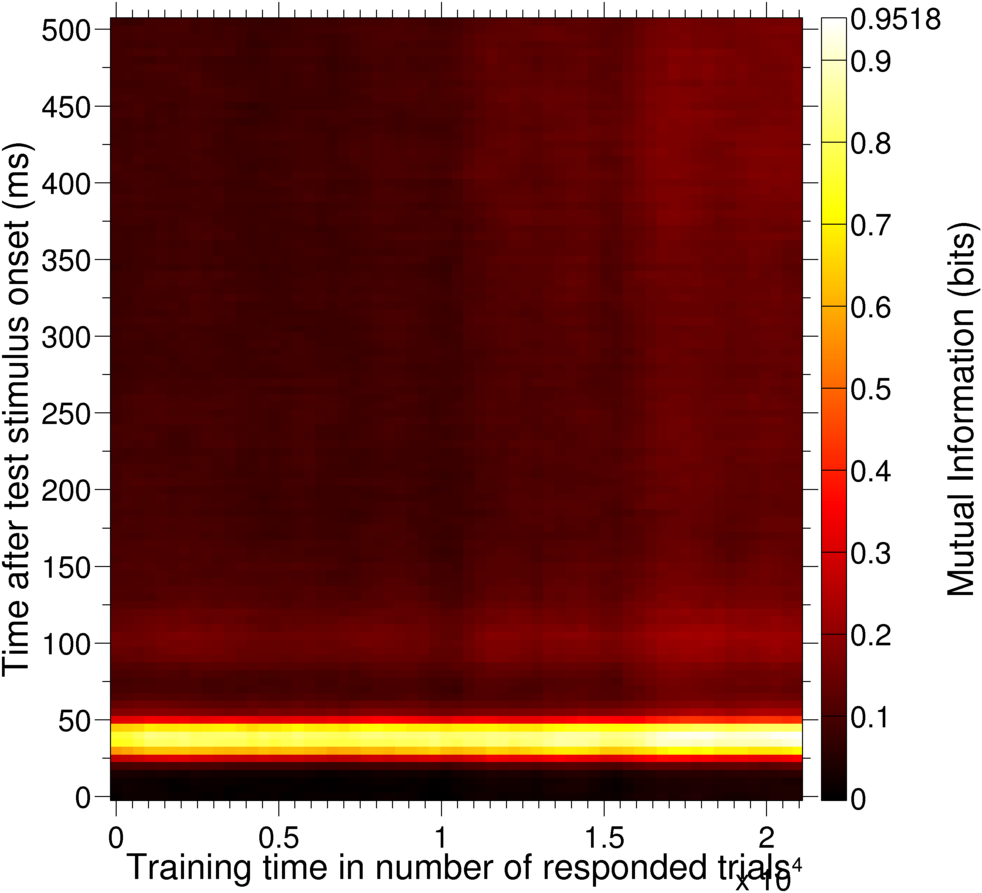
\includegraphics[scale=.25]{%
% % ./figs/I_trialwise_jack_v1_chmean25_s51-72_tp4_5bins_of_4ms_dr_pt_oc0_test_tc5-5-20,22-3-28,32,35-5-50,60,90_nt1400_ts350_rmvet1_rmvms1_pcolorhot_20120815T234434.png}
% %     \end{subfigure}
% %     ~~
% %     \begin{subfigure}[b]{0.5\linewidth}
% %         \centering
% %         \caption{}
% %         \label{fig:j1-5x4tp1}
% %         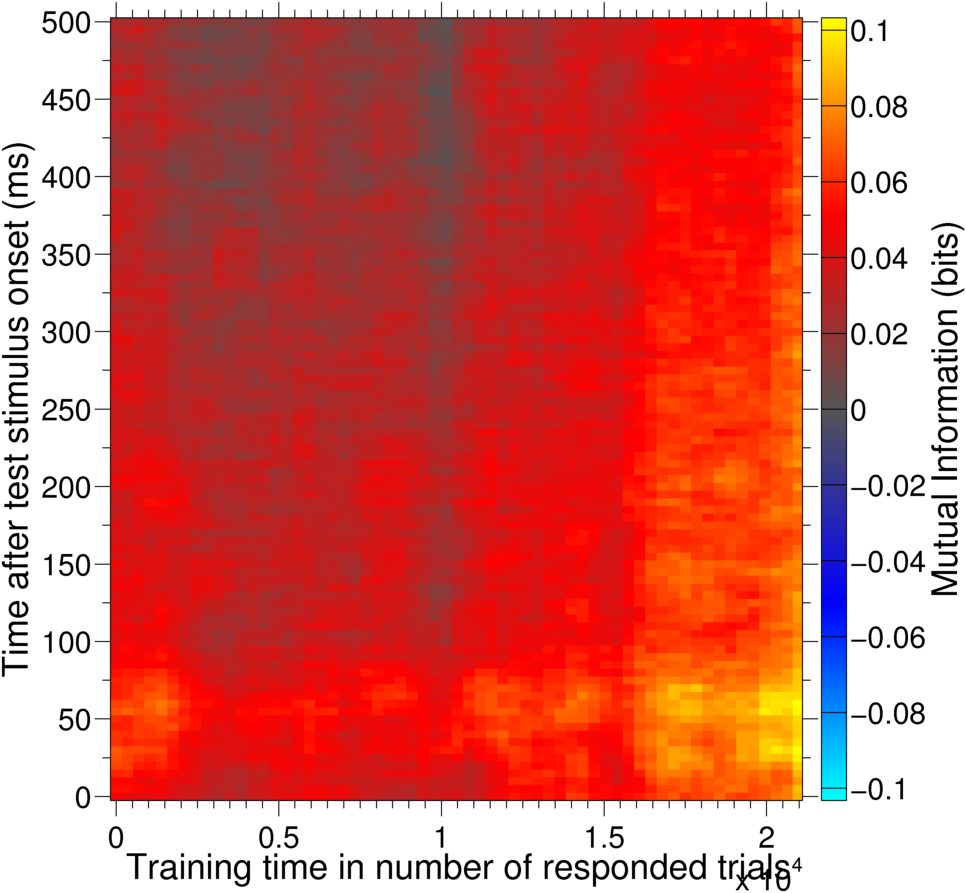
\includegraphics[scale=.25]{%
% % ./figs/I_trialwise_jack_v1_chmean25_s51-72_tp1_5bins_of_4ms_dr_pt_oc0_test_tc5-5-20,22-3-28,32,35-5-50,60,90_nt1400_ts350_rmvet1_rmvms1_pcolorbp_20120816T175343.png}
% %     \end{subfigure}
% %     \caption{M2 V1: Mutual information between the test stimulus and \unit[20]{ms} of spiking activity, averaged across 25 channels.
% % The PT bias correction method was used in all estimates of the information.
% % Panels \ref{fig:j1-1x20tp4}--\ref{fig:j1-5x4tp1} are the same as for Fig.~\ref{fig:b1-trialwise}.
% % % The neural code used in \ref{fig:j1-1x20tp4ma}--\ref{fig:j1-1x20tp1} is a spike count code, whilst in \ref{fig:j1-5x4tp4}, \ref{fig:j1-5x4tp1} it is a spike timing code where the \unit[20]{ms} window was subdivided into 5 bins each of \unit[4]{ms}.
% % % In \ref{fig:j1-1x20tp4ma}, \ref{fig:j1-1x20tp4}, and \ref{fig:j1-5x4tp4}, the spike-train is taken from the test presentation part of the trial;
% % % for \ref{fig:j1-1x20tp1ma}, \ref{fig:j1-1x20tp1}, and \ref{fig:j1-5x4tp1}, the spike-train is taken from spontaneous pre-stimulus activity.
% % % In \ref{fig:j1-1x20tp4ma} and \ref{fig:j1-1x20tp1ma} no attempt was made to remove the monitor artifact from the raw data, whilst in the rest of the panels the data was modified to counter this as described in \ref{sec:ma}.
% % % \ref{fig:j1-1x20tp4ma}
% % % \ref{fig:j1-1x20tp1ma}
% % % \ref{fig:j1-1x20tp4}
% % % \ref{fig:j1-1x20tp1}
% % % \ref{fig:j1-5x4tp4}
% % % \ref{fig:j1-5x4tp1}
% % }
% %     \label{fig:j1-trialwise}
% % \end{figure}

% ./figs/I_trialwise_blanco_v4_chmean31_s307,308,311,313,314,317,318,320,321,329-341_tp4_1bins_of_20ms_dr_pt_oc0_test_tc10-5-25,27-29,31-33,35,40-10-60_nt1400_ts350_rmvet1_rmvms0_pcolorhot_20120815T234508.png
% ./figs/I_trialwise_blanco_v4_chmean31_s307,308,311,313,314,317,318,320,321,329-341_tp1_1bins_of_20ms_dr_pt_oc0_test_tc10-5-25,27-29,31-33,35,40-10-60_nt1400_ts350_rmvet1_rmvms0_pcolorhot_20120815T234341.png
% ./figs/I_trialwise_blanco_v4_chmean31_s307,308,311,313,314,317,318,320,321,329-341_tp4_1bins_of_20ms_dr_pt_oc0_test_tc10-5-25,27-29,31-33,35,40-10-60_nt1400_ts350_rmvet1_rmvms1_pcolorhot_20120815T234756.png
% ./figs/I_trialwise_blanco_v4_chmean31_s307,308,311,313,314,317,318,320,321,329-341_tp1_1bins_of_20ms_dr_pt_oc0_test_tc10-5-25,27-29,31-33,35,40-10-60_nt1400_ts350_rmvet1_rmvms1_pcolorbp_20120816T175507.png
% ./figs/I_trialwise_blanco_v4_chmean31_s307,308,311,313,314,317,318,320,321,329-341_tp4_5bins_of_4ms_dr_pt_oc0_test_tc10-5-25,27-29,31-33,35,40-10-60_nt1400_ts350_rmvet1_rmvms1_pcolorhot_20120815T234528.png
% ./figs/I_trialwise_blanco_v4_chmean31_s307,308,311,313,314,317,318,320,321,329-341_tp1_5bins_of_4ms_dr_pt_oc0_test_tc10-5-25,27-29,31-33,35,40-10-60_nt1400_ts350_rmvet1_rmvms1_pcolorbp_20120816T175438.png

% % \cleartoevenpage

% % \begin{figure}[htbp]
% % %     \begin{subfigure}[b]{0.5\linewidth}
% % %         \centering
% % %         \includegraphics[scale=.25]{%
% % % ./figs/I_trialwise_blanco_v4_chmean31_s307,308,311,313,314,317,318,320,321,329-341_tp4_1bins_of_20ms_dr_pt_oc0_test_tc10-5-25,27-29,31-33,35,40-10-60_nt1400_ts350_rmvet1_rmvms0_pcolorhot_20120815T234508.png}
% % %         \caption{}
% % %         \label{fig:b4-1x20tp4ma}
% % %     \end{subfigure}
% % %     ~~
% % %     \begin{subfigure}[b]{0.5\linewidth}
% % %         \centering
% % %         \includegraphics[scale=.25]{%
% % % ./figs/I_trialwise_blanco_v4_chmean31_s307,308,311,313,314,317,318,320,321,329-341_tp1_1bins_of_20ms_dr_pt_oc0_test_tc10-5-25,27-29,31-33,35,40-10-60_nt1400_ts350_rmvet1_rmvms0_pcolorhot_20120815T234341.png}
% % %         \caption{}
% % %         \label{fig:b4-1x20tp1ma}
% % %     \end{subfigure}
% % %     \\
% %     \begin{subfigure}[b]{0.5\linewidth}
% %         \centering
% %         \caption{}
% %         \label{fig:b4-1x20tp4}
% %         \includegraphics[scale=.25]{%
% % ./figs/I_trialwise_blanco_v4_chmean31_s307,308,311,313,314,317,318,320,321,329-341_tp4_1bins_of_20ms_dr_pt_oc0_test_tc10-5-25,27-29,31-33,35,40-10-60_nt1400_ts350_rmvet1_rmvms1_pcolorhot_20120815T234756.png}
% %     \end{subfigure}
% %     ~~
% %     \begin{subfigure}[b]{0.5\linewidth}
% %         \centering
% %         \caption{}
% %         \label{fig:b4-1x20tp1}
% %         \includegraphics[scale=.25]{%
% % ./figs/I_trialwise_blanco_v4_chmean31_s307,308,311,313,314,317,318,320,321,329-341_tp1_1bins_of_20ms_dr_pt_oc0_test_tc10-5-25,27-29,31-33,35,40-10-60_nt1400_ts350_rmvet1_rmvms1_pcolorbp_20120816T175507.png}
% %     \end{subfigure}
% %     \\
% %     \begin{subfigure}[b]{0.5\linewidth}
% %         \centering
% %         \caption{}
% %         \label{fig:b4-5x4tp4}
% %         \includegraphics[scale=.25]{%
% % ./figs/I_trialwise_blanco_v4_chmean31_s307,308,311,313,314,317,318,320,321,329-341_tp4_5bins_of_4ms_dr_pt_oc0_test_tc10-5-25,27-29,31-33,35,40-10-60_nt1400_ts350_rmvet1_rmvms1_pcolorhot_20120815T234528.png}
% %     \end{subfigure}
% %     ~~
% %     \begin{subfigure}[b]{0.5\linewidth}
% %         \centering
% %         \caption{}
% %         \label{fig:b4-5x4tp1}
% %         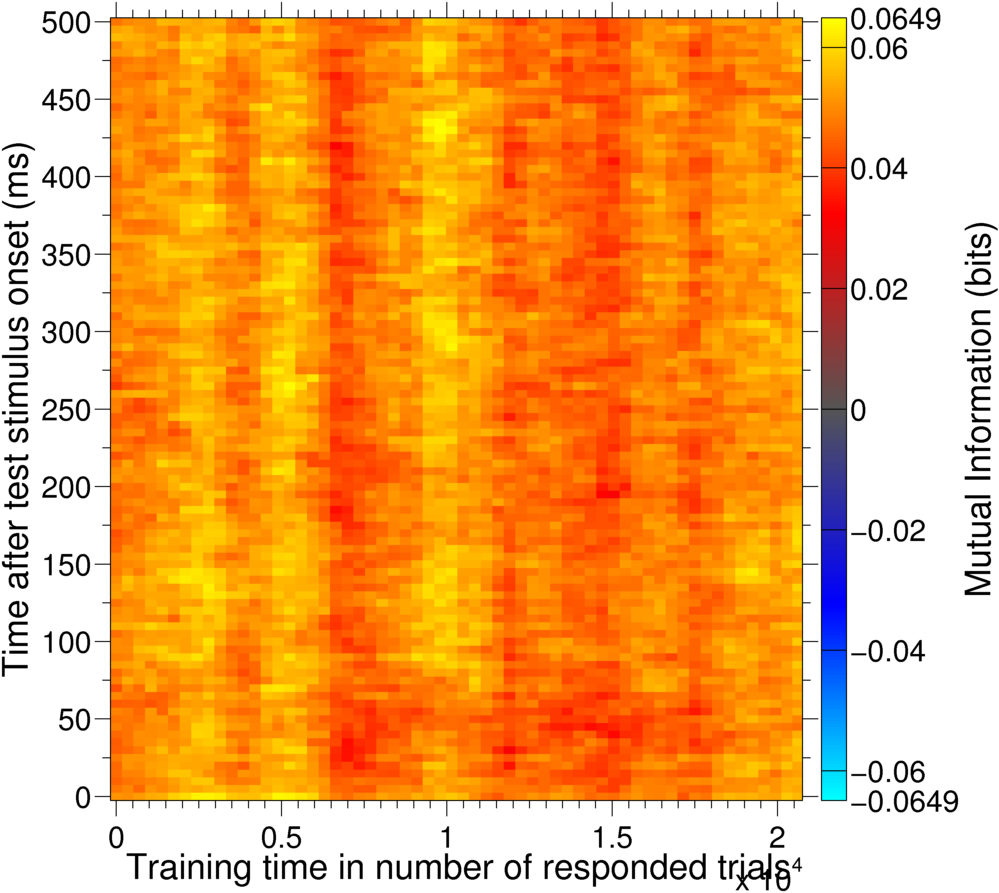
\includegraphics[scale=.25]{%
% % ./figs/I_trialwise_blanco_v4_chmean31_s307,308,311,313,314,317,318,320,321,329-341_tp1_5bins_of_4ms_dr_pt_oc0_test_tc10-5-25,27-29,31-33,35,40-10-60_nt1400_ts350_rmvet1_rmvms1_pcolorbp_20120816T175438.png}
% %     \end{subfigure}
% %     \caption{M1 V4: Mutual information between the test stimulus and \unit[20]{ms} of spiking activity, averaged across 30 channels.
% % The PT bias correction method was used in all estimates of the information.
% % Panels \ref{fig:b4-1x20tp4}--\ref{fig:b4-5x4tp1} are the same as for Fig.~\ref{fig:b1-trialwise}.
% % % The neural code used in \ref{fig:b4-1x20tp4ma}--\ref{fig:b4-1x20tp1} is a spike count code, whilst in \ref{fig:b4-5x4tp4}, \ref{fig:b4-5x4tp1} it is a spike timing code where the \unit[20]{ms} window was subdivided into 5 bins each of \unit[4]{ms}.
% % % In \ref{fig:b4-1x20tp4ma}, \ref{fig:b4-1x20tp4}, and \ref{fig:b4-5x4tp4}, the spike-train is taken from the test presentation part of the trial;
% % % for \ref{fig:b4-1x20tp1ma}, \ref{fig:b4-1x20tp1}, and \ref{fig:b4-5x4tp1}, the spike-train is taken from spontaneous pre-stimulus activity.
% % % In \ref{fig:b4-1x20tp4ma} and \ref{fig:b4-1x20tp1ma} no attempt was made to remove the monitor artifact from the raw data, whilst in the rest of the panels the data was modified to counter this as described in \ref{sec:ma}.
% % % \ref{fig:b4-1x20tp4ma}
% % % \ref{fig:b4-1x20tp1ma}
% % % \ref{fig:b4-1x20tp4}
% % % \ref{fig:b4-1x20tp1}
% % % \ref{fig:b4-5x4tp4}
% % % \ref{fig:b4-5x4tp1}
% % }
% %     \label{fig:b4-trialwise}
% % \end{figure}



% ./figs/I_trialwise_jack_v4_chmean20_s24-49_tp4_1bins_of_20ms_dr_pt_oc0_test_tc10-5-25,27-29,31-33,35,40-10-60_nt1400_ts350_rmvet1_rmvms0_pcolorhot_20120815T234433.png
% ./figs/I_trialwise_jack_v4_chmean20_s24-49_tp1_1bins_of_20ms_dr_pt_oc0_test_tc10-5-25,27-29,31-33,35,40-10-60_nt1400_ts350_rmvet1_rmvms1_pcolorbp_20120816T175433.png
% ./figs/I_trialwise_jack_v4_chmean20_s24-49_tp4_1bins_of_20ms_dr_pt_oc0_test_tc10-5-25,27-29,31-33,35,40-10-60_nt1400_ts350_rmvet1_rmvms1_pcolorhot_20120815T234723.png
% ./figs/I_trialwise_jack_v4_chmean20_s24-49_tp1_1bins_of_20ms_dr_pt_oc0_test_tc10-5-25,27-29,31-33,35,40-10-60_nt1400_ts350_rmvet1_rmvms1_pcolorhot_20120815T234559.png
% ./figs/I_trialwise_jack_v4_chmean20_s24-49_tp4_5bins_of_4ms_dr_pt_oc0_test_tc10-5-25,27-29,31-33,35,40-10-60_nt1400_ts350_rmvet1_rmvms1_pcolorhot_20120815T234455.png
% ./figs/I_trialwise_jack_v4_chmean20_s24-49_tp1_5bins_of_4ms_dr_pt_oc0_test_tc10-5-25,27-29,31-33,35,40-10-60_nt1400_ts350_rmvet1_rmvms1_pcolorbp_20120816T175404.png

% % \begin{figure}[htbp]
% % %     \begin{subfigure}[b]{0.5\linewidth}
% % %         \centering
% % %         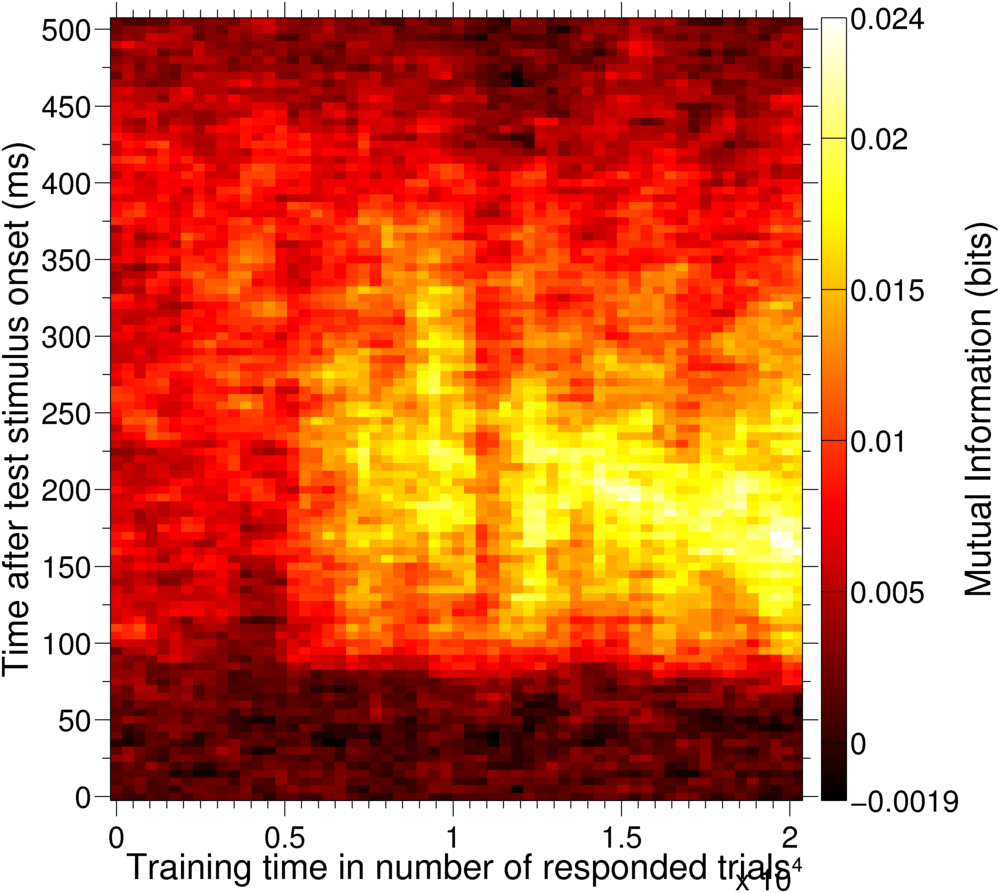
\includegraphics[scale=.25]{%
% % % ./figs/I_trialwise_jack_v4_chmean20_s24-49_tp4_1bins_of_20ms_dr_pt_oc0_test_tc10-5-25,27-29,31-33,35,40-10-60_nt1400_ts350_rmvet1_rmvms0_pcolorhot_20120815T234433.png}
% % %         \caption{}
% % %         \label{fig:j4-1x20tp4ma}
% % %     \end{subfigure}
% % %     ~~
% % %     \begin{subfigure}[b]{0.5\linewidth}
% % %         \centering
% % %         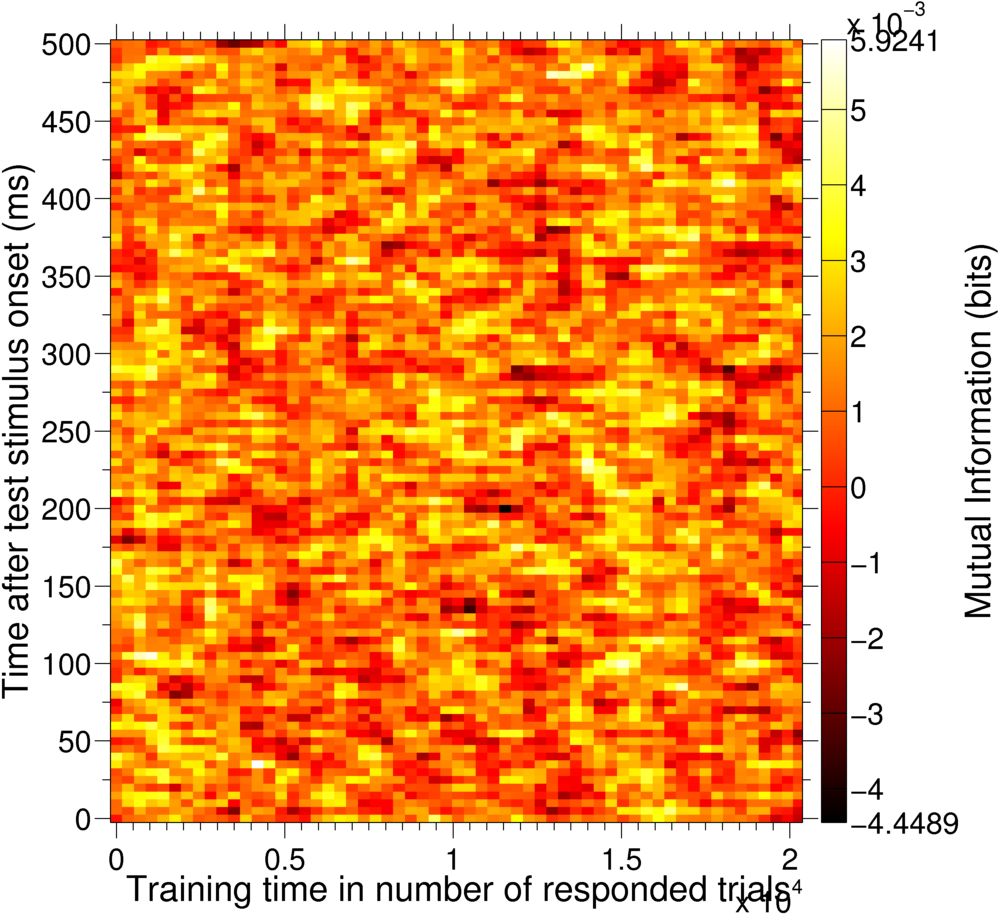
\includegraphics[scale=.25]{%
% % % ./figs/I_trialwise_jack_v4_chmean20_s24-49_tp1_1bins_of_20ms_dr_pt_oc0_test_tc10-5-25,27-29,31-33,35,40-10-60_nt1400_ts350_rmvet1_rmvms0_pcolorhot_20120815T234307.png}
% % %         \caption{}
% % %         \label{fig:j4-1x20tp1ma}
% % %     \end{subfigure}
% % %     \\
% %     \begin{subfigure}[b]{0.5\linewidth}
% %         \centering
% %         \caption{}
% %         \label{fig:j4-1x20tp4}
% %         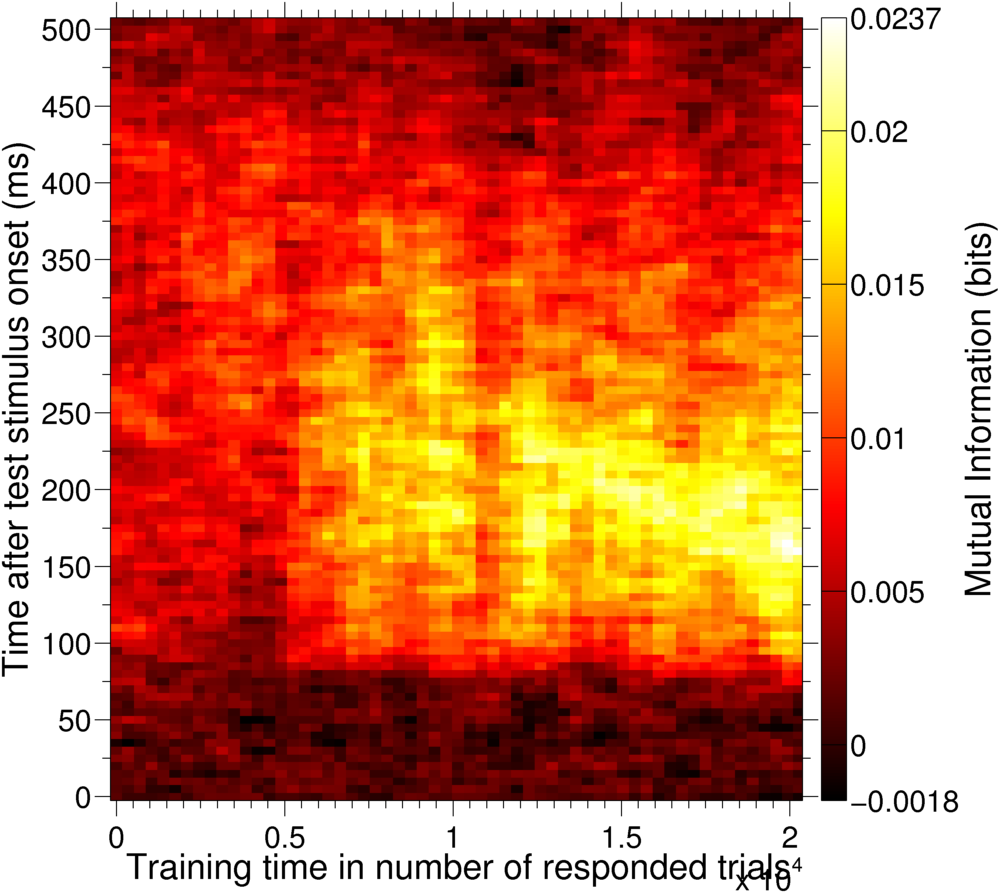
\includegraphics[scale=.25]{%
% % ./figs/I_trialwise_jack_v4_chmean20_s24-49_tp4_1bins_of_20ms_dr_pt_oc0_test_tc10-5-25,27-29,31-33,35,40-10-60_nt1400_ts350_rmvet1_rmvms1_pcolorhot_20120815T234723.png}
% %     \end{subfigure}
% %     ~~
% %     \begin{subfigure}[b]{0.5\linewidth}
% %         \centering
% %         \caption{}
% %         \label{fig:j4-1x20tp1}
% %         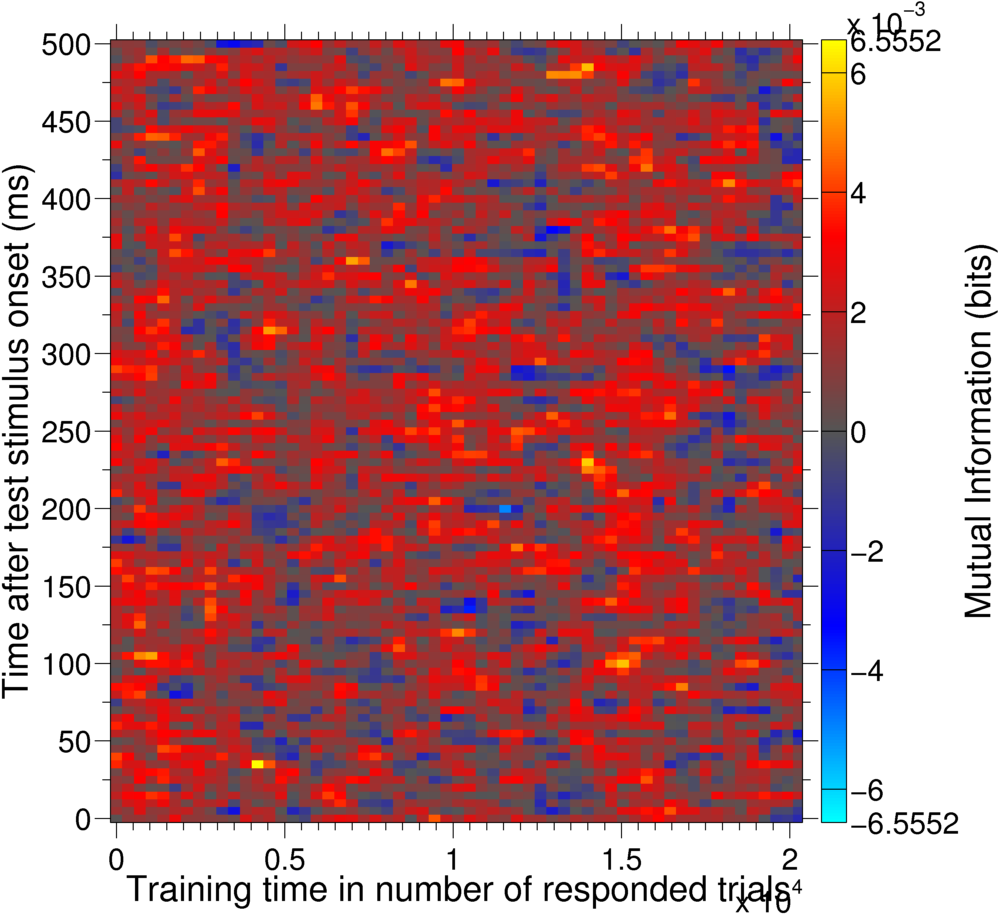
\includegraphics[scale=.25]{%
% % ./figs/I_trialwise_jack_v4_chmean20_s24-49_tp1_1bins_of_20ms_dr_pt_oc0_test_tc10-5-25,27-29,31-33,35,40-10-60_nt1400_ts350_rmvet1_rmvms1_pcolorbp_20120816T175433.png}
% %     \end{subfigure}
% %     \\
% %     \begin{subfigure}[b]{0.5\linewidth}
% %         \centering
% %         \caption{}
% %         \label{fig:j4-5x4tp4}
% %         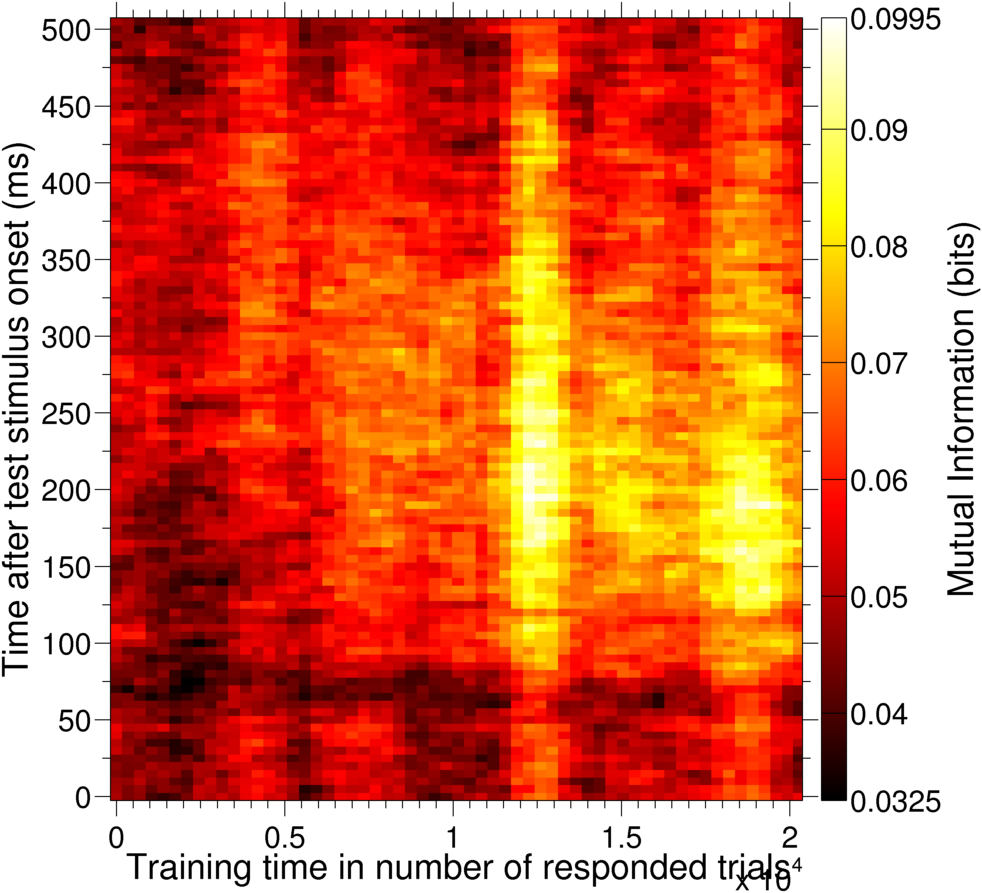
\includegraphics[scale=.25]{%
% % ./figs/I_trialwise_jack_v4_chmean20_s24-49_tp4_5bins_of_4ms_dr_pt_oc0_test_tc10-5-25,27-29,31-33,35,40-10-60_nt1400_ts350_rmvet1_rmvms1_pcolorhot_20120815T234455.png}
% %     \end{subfigure}
% %     ~~
% %     \begin{subfigure}[b]{0.5\linewidth}
% %         \centering
% %         \caption{}
% %         \label{fig:j4-5x4tp1}
% %         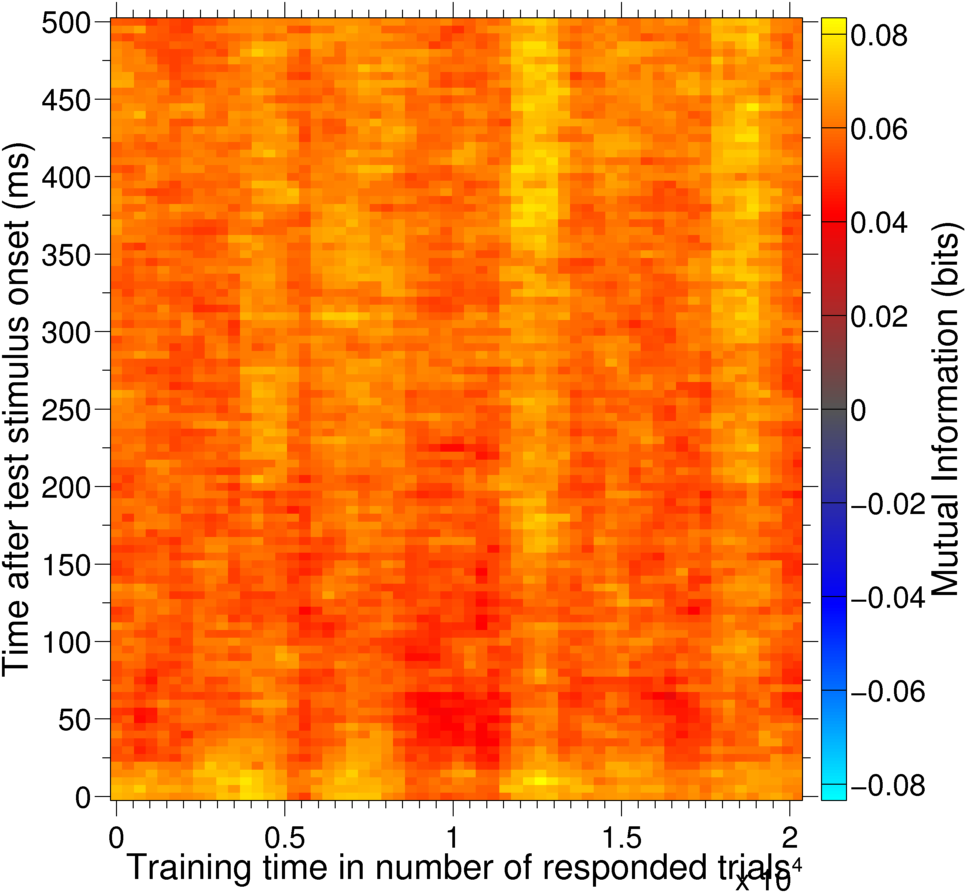
\includegraphics[scale=.25]{%
% % ./figs/I_trialwise_jack_v4_chmean20_s24-49_tp1_5bins_of_4ms_dr_pt_oc0_test_tc10-5-25,27-29,31-33,35,40-10-60_nt1400_ts350_rmvet1_rmvms1_pcolorbp_20120816T175404.png}
% %     \end{subfigure}
% %     \caption{M2 V4: Mutual information between the test stimulus and \unit[20]{ms} of spiking activity, averaged across 20 channels.
% % The PT bias correction method was used in all estimates of the information.
% % Panels \ref{fig:j4-1x20tp4}--\ref{fig:j4-5x4tp1} are the same as for Fig.~\ref{fig:b1-trialwise}.
% % % The neural code used in \ref{fig:j4-1x20tp4ma}--\ref{fig:j4-1x20tp1} is a spike count code, whilst in \ref{fig:j4-5x4tp4}, \ref{fig:j4-5x4tp1} it is a spike timing code where the \unit[20]{ms} window was subdivided into 5 bins each of \unit[4]{ms}.
% % % In \ref{fig:j4-1x20tp4ma}, \ref{fig:j4-1x20tp4}, and \ref{fig:j4-5x4tp4}, the spike-train is taken from the test presentation part of the trial;
% % % for \ref{fig:j4-1x20tp1ma}, \ref{fig:j4-1x20tp1}, and \ref{fig:j4-5x4tp1}, the spike-train is taken from spontaneous pre-stimulus activity.
% % % In \ref{fig:j4-1x20tp4ma} and \ref{fig:j4-1x20tp1ma} no attempt was made to remove the monitor artifact from the raw data, whilst in the rest of the panels the data was modified to counter this as described in \ref{sec:ma}.
% % % \ref{fig:j4-1x20tp4ma}
% % % \ref{fig:j4-1x20tp1ma}
% % % \ref{fig:j4-1x20tp4}
% % % \ref{fig:j4-1x20tp1}
% % % \ref{fig:j4-5x4tp4}
% % % \ref{fig:j4-5x4tp1}
% % }
% %     \label{fig:j4-trialwise}
% % \end{figure}

% 20, 30 and \unit[40]{ms} all tried. Mutual information increases as the duration increases as one would expect, but there is no other significant difference. Consequently only 20ms is shown in this section.

% More information with only correct trials used, but this could be due to differences in $P(S)$.

Turning our attention to the V4 results in Figs.~\ref{fig:b4-trialwise} and \ref{fig:j4-trialwise}, we can see the effect of the transient is present in M1's data (at the later start time of \unit[75]{ms}), but not in M2's. This is surprising because, looking at the rasters, in both animals there are some channels which exhibit a transient response and some which do not.

Similar to V1, it seems as if there is four times as much information in the timebinned code compared with the count code. However, there is much more information measured for the spontaneous activity data again. This is not reduced by increasing the number of trials either.

For the spike count code in M2, the spontaneous information is nearly distributed around 0, suggesting the bias has been all but removed and the data is of very high quality. For this animal, we can see a distinct increase in the information content with time, for both the spike count and timing codes. Simultaneously, there is a movement of the peak information to earlier times closer to the stimulus onset.

In M1, there is a small increase in the information content with time which may or may not significant. However, it is reassuring to see that this is not due to an improvement in the data with time, as the trend in the spontaneous activity information bias (Fig.~\ref{fig:j4-5x4tp1}) is a decrease with time.

%----------------------------------------------------------------------------------------------------------------------
\FloatBarrier
\subsubsection{Fine vs coarse contrast differences}

Comparing Figs.~\ref{fig:b1-1x20cc} and \ref{fig:j1-1x20cc} where the outer 6 contrasts are included with Figs.~\ref{fig:b1-1x20tp4} and \ref{fig:b1-1x20tp4} where all contrasts are included, it seems as if the amount of information has increased, which should not be possible. However, the difference will be due to the difference in trials contained in each of the analyses. In each case, an average of 100 trials per stimulus is used, but since the easier test conditions are presented less frequently, they are under-represented in Figs.~\ref{fig:b1-1x20tp4} and \ref{fig:b1-1x20tp4} (about 75 trials per stimulus). Obviously these are more discriminable, so the under-representation comparably reduces the information.

Looking at V1 (Fig.~\ref{fig:v1-fvc}), we observe there is much more information for M2 than M1, as we found before. The quality of the data seems to have severely hampered the analysis for M1, destroying the the fine differences in the data needed to evaluate the information contained about fine contrast differences (Fig.~\ref{fig:b1-1x20fc}).

Unsurprisingly, there is more information when considering the coarsely distinct contrasts than the finer differences, as the neural activity is bound to be more discriminable for these. For M2, there is a small upward trend again for both coarse and fine contrast differences, which may or may not be genuine.

% ./figs/I_trialwise_blanco_v1_chmean23_s343-354,355.1,355.2,356-359_tp4_1bins_of_20ms_dr_pt_oc0_test_tc5,15,22,40,50,90_nt600_ts150_rmvet1_rmvms1_pcolorhot_20120816T011936.png
% ./figs/I_trialwise_blanco_v1_chmean23_s343-354,355.1,355.2,356-359_tp4_1bins_of_20ms_dr_pt_oc0_test_tc22-3-28,32,35,40_nt600_ts150_rmvet1_rmvms1_pcolorhot_20120816T011920.png
% ./figs/I_trialwise_jack_v1_chmean25_s51-72_tp4_1bins_of_20ms_dr_pt_oc0_test_tc5,15,22,40,50,90_nt600_ts150_rmvet1_rmvms1_pcolorhot_20120816T011822.png
% ./figs/I_trialwise_jack_v1_chmean25_s51-72_tp4_1bins_of_20ms_dr_pt_oc0_test_tc22-3-28,32,35,40_nt600_ts150_rmvet1_rmvms1_pcolorhot_20120816T011800.png

% % \begin{figure}[htbp]
% %     \begin{subfigure}[b]{0.5\linewidth}
% %         \centering
% %         \caption{}
% %         \label{fig:b1-1x20cc}
% %         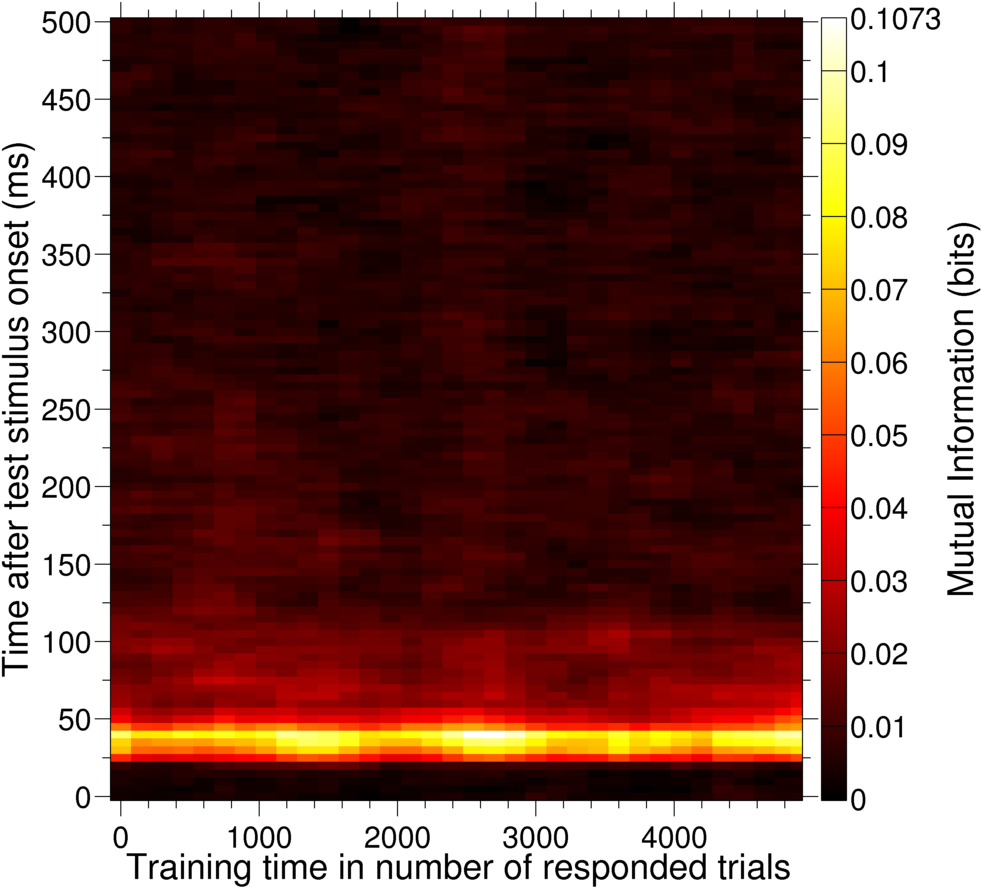
\includegraphics[scale=.25]{%
% % ./figs/I_trialwise_blanco_v1_chmean23_s343-354,355.1,355.2,356-359_tp4_1bins_of_20ms_dr_pt_oc0_test_tc5,15,22,40,50,90_nt600_ts150_rmvet1_rmvms1_pcolorhot_20120816T011936.png}
% %     \end{subfigure}
% %     ~~
% %     \begin{subfigure}[b]{0.5\linewidth}
% %         \centering
% %         \caption{}
% %         \label{fig:j1-1x20cc}
% %         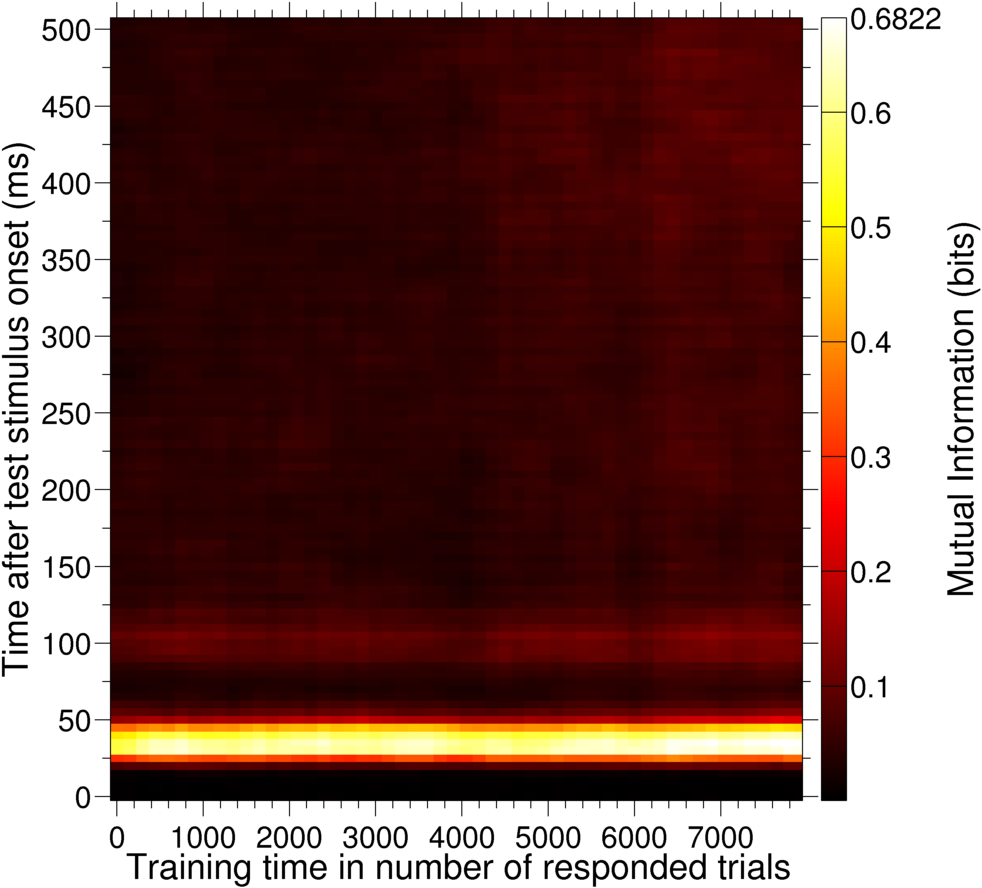
\includegraphics[scale=.25]{%
% % ./figs/I_trialwise_jack_v1_chmean25_s51-72_tp4_1bins_of_20ms_dr_pt_oc0_test_tc5,15,22,40,50,90_nt600_ts150_rmvet1_rmvms1_pcolorhot_20120816T011822.png}
% %     \end{subfigure}
% %     \\
% %     \begin{subfigure}[b]{0.5\linewidth}
% %         \centering
% %         \caption{}
% %         \label{fig:b1-1x20fc}
% %         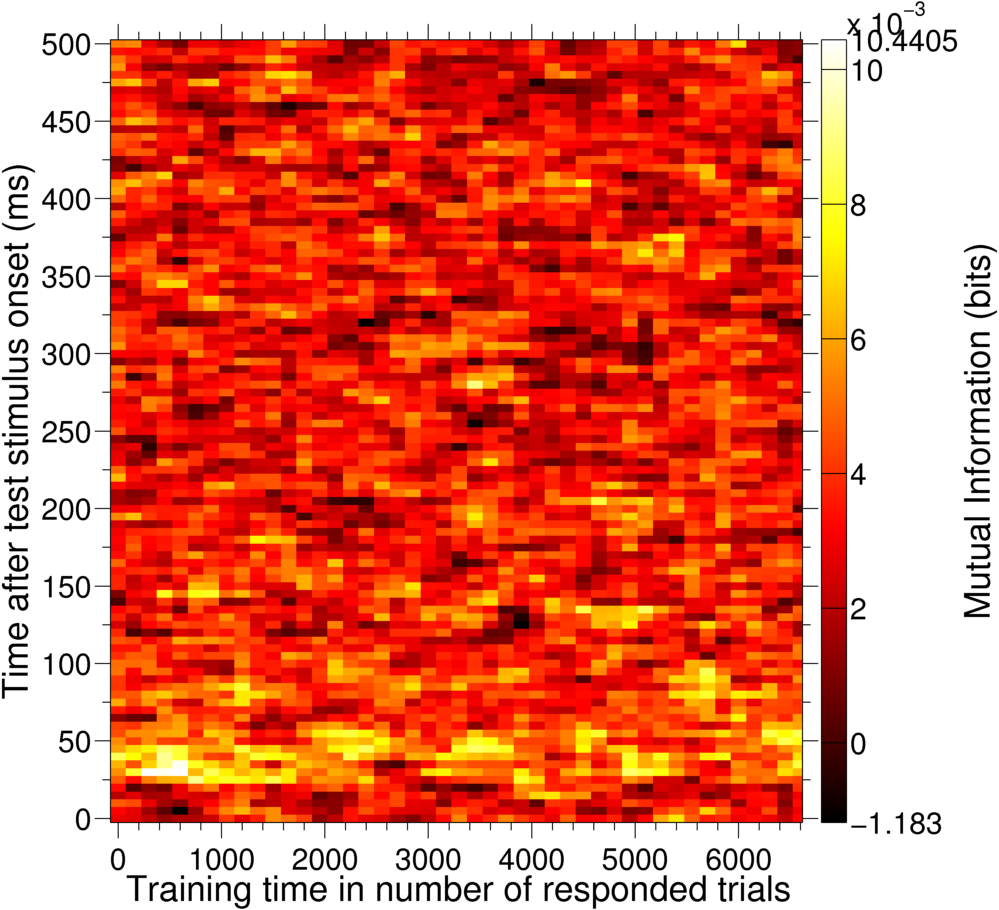
\includegraphics[scale=.25]{%
% % ./figs/I_trialwise_blanco_v1_chmean23_s343-354,355.1,355.2,356-359_tp4_1bins_of_20ms_dr_pt_oc0_test_tc22-3-28,32,35,40_nt600_ts150_rmvet1_rmvms1_pcolorhot_20120816T011920.png}
% %     \end{subfigure}
% %     ~~
% %     \begin{subfigure}[b]{0.5\linewidth}
% %         \centering
% %         \caption{}
% %         \label{fig:j1-1x20fc}
% %         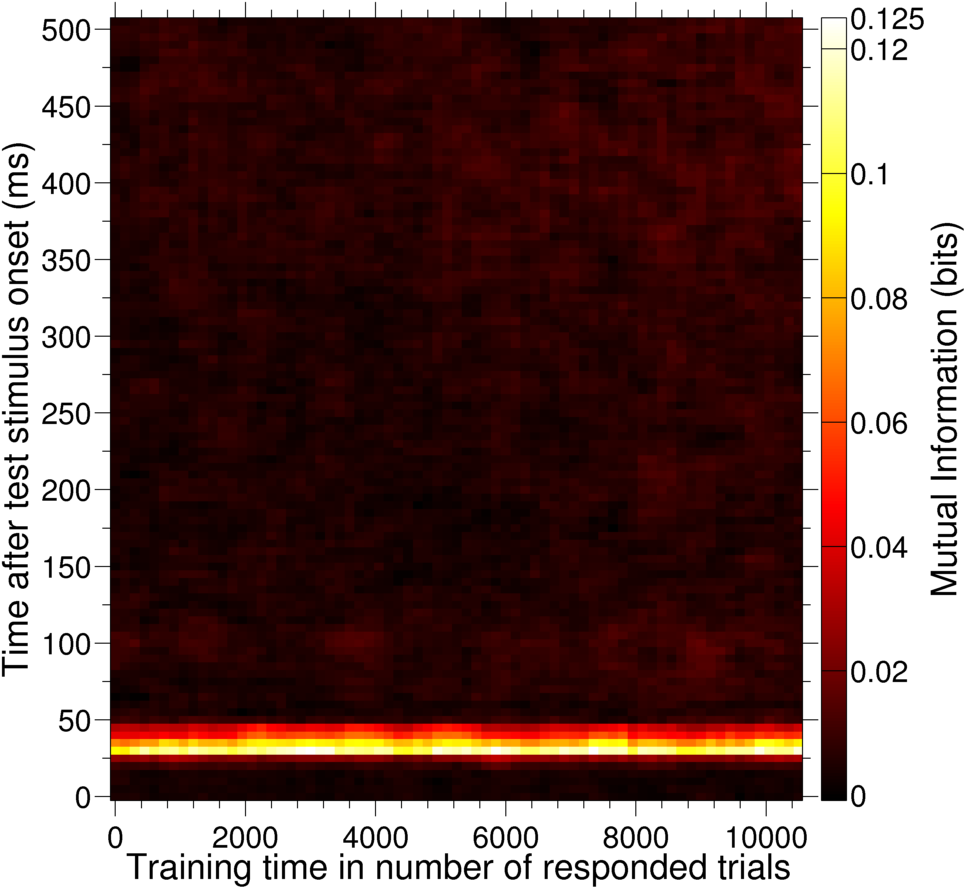
\includegraphics[scale=.25]{%
% % ./figs/I_trialwise_jack_v1_chmean25_s51-72_tp4_1bins_of_20ms_dr_pt_oc0_test_tc22-3-28,32,35,40_nt600_ts150_rmvet1_rmvms1_pcolorhot_20120816T011800.png}
% %     \end{subfigure}
% %     \caption{V1: Fine vs. coarse contrast differences.
% % % Mutual information between the test stimulus and \unit[20]{ms} of spiking activity.
% % % The PT bias correction method was used in all estimates of the information.
% % In the top panels, the six contrasts included are \{5, 15, 22, 40, 50, 90\}\%; bottom panels \{22, 25, 28, 32, 35, 40\}\%. An average of 100 trials per stimulus is used in each of these.
% % Left panels are for M1, right are M2.
% % In each case, mutual information between the six test stimuli and \unit[20]{ms} of spiking activity was measured using a spike count code, and bias corrected using the PT method.
% % % Panels \ref{fig:b1-1x20cc} and \ref{fig:b1-1x20fc} are for M1, \ref{fig:b1-1x20cc} and \ref{fig:b1-1x20fc} for M2.
% % }
% %     \label{fig:v1-fvc}
% % \end{figure}


% ./figs/I_trialwise_blanco_v4_chmean31_s307,308,311,313,314,317,318,320,321,329-341_tp4_1bins_of_20ms_dr_pt_oc0_test_tc10-5-20,40-10-60_nt600_ts150_rmvet1_rmvms1_pcolorhot_20120816T012120.png
% ./figs/I_trialwise_blanco_v4_chmean31_s307,308,311,313,314,317,318,320,321,329-341_tp4_1bins_of_20ms_dr_pt_oc0_test_tc27-29,31-33_nt600_ts150_rmvet1_rmvms1_pcolorhot_20120816T011952.png
% ./figs/I_trialwise_jack_v4_chmean20_s24-49_tp4_1bins_of_20ms_dr_pt_oc0_test_tc10-5-20,40-10-60_nt600_ts150_rmvet1_rmvms1_pcolorhot_20120816T011902.png
% ./figs/I_trialwise_jack_v4_chmean20_s24-49_tp4_1bins_of_20ms_dr_pt_oc0_test_tc27-29,31-33_nt600_ts150_rmvet1_rmvms1_pcolorhot_20120816T011843.png

% % \begin{figure}[htbp]
% %     \begin{subfigure}[b]{0.5\linewidth}
% %         \centering
% %         \caption{}
% %         \label{fig:b4-1x20cc}
% %         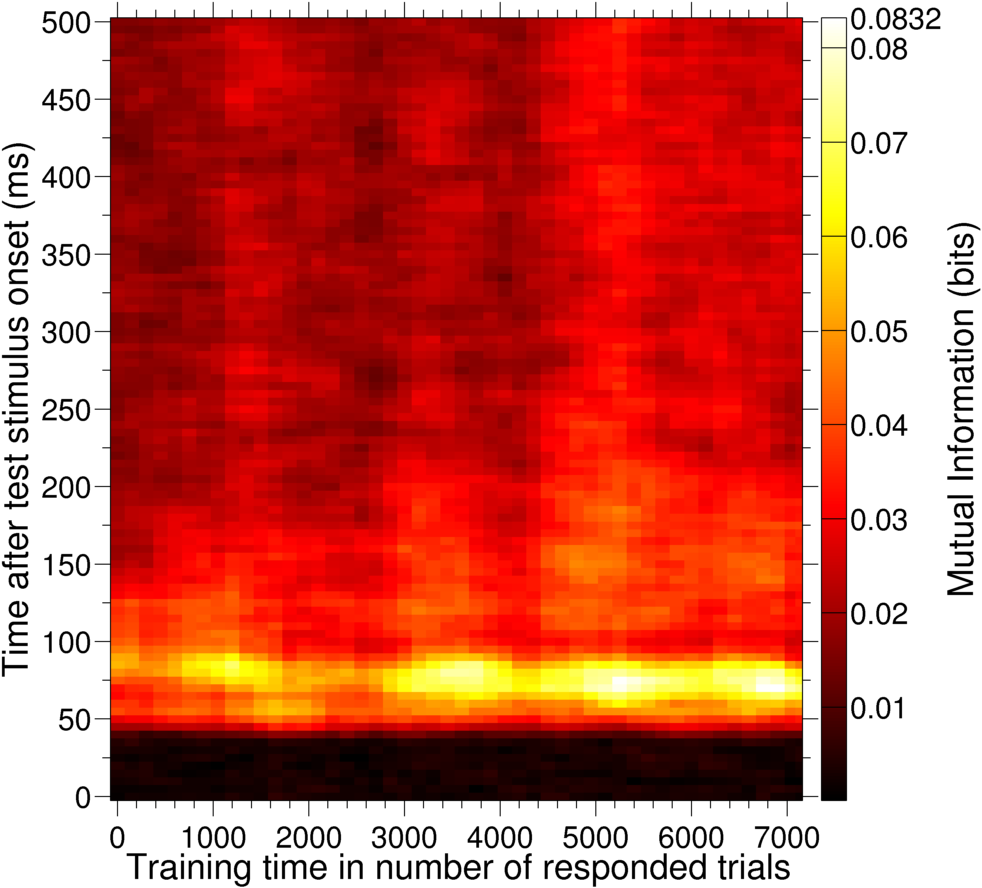
\includegraphics[scale=.25]{%
% % ./figs/I_trialwise_blanco_v4_chmean31_s307,308,311,313,314,317,318,320,321,329-341_tp4_1bins_of_20ms_dr_pt_oc0_test_tc10-5-20,40-10-60_nt600_ts150_rmvet1_rmvms1_pcolorhot_20120816T012120.png}
% %     \end{subfigure}
% %     ~~
% %     \begin{subfigure}[b]{0.5\linewidth}
% %         \centering
% %         \caption{}
% %         \label{fig:j4-1x20cc}
% %         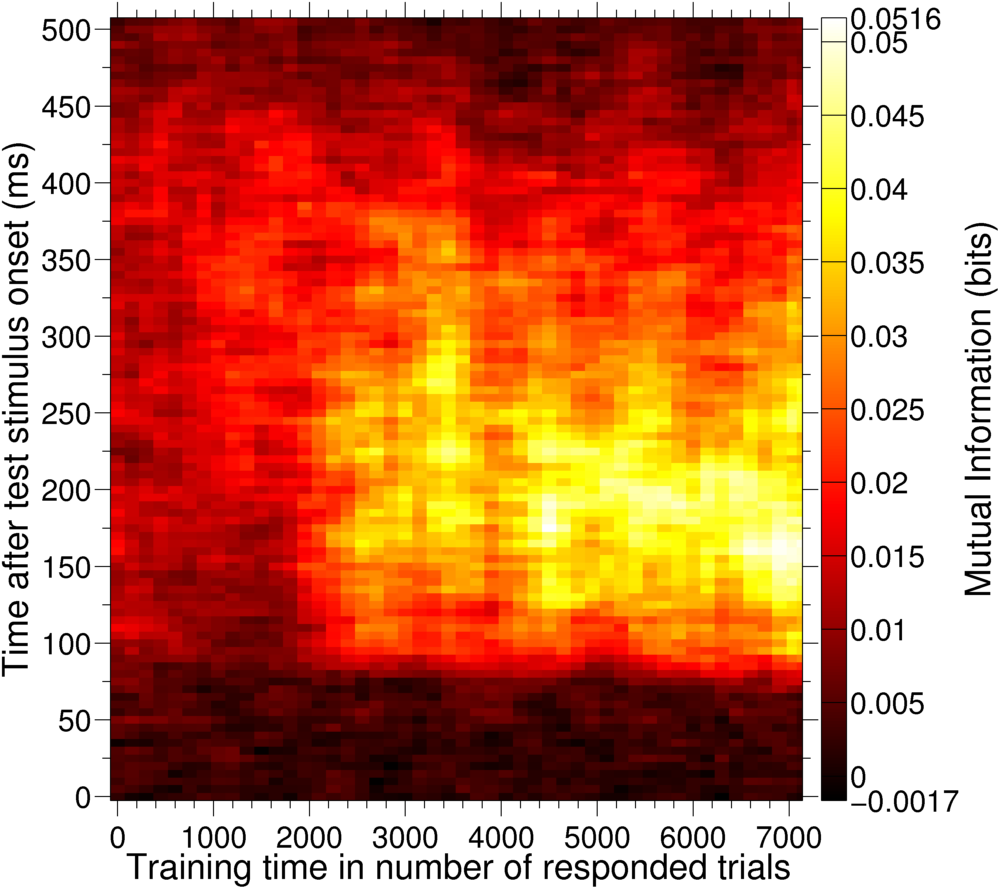
\includegraphics[scale=.25]{%
% % ./figs/I_trialwise_jack_v4_chmean20_s24-49_tp4_1bins_of_20ms_dr_pt_oc0_test_tc10-5-20,40-10-60_nt600_ts150_rmvet1_rmvms1_pcolorhot_20120816T011902.png}
% %     \end{subfigure}
% %     \\
% %     \begin{subfigure}[b]{0.5\linewidth}
% %         \centering
% %         \caption{}
% %         \label{fig:b4-1x20fc}
% %         \includegraphics[scale=.25]{%
% % ./figs/I_trialwise_blanco_v4_chmean31_s307,308,311,313,314,317,318,320,321,329-341_tp4_1bins_of_20ms_dr_pt_oc0_test_tc27-29,31-33_nt600_ts150_rmvet1_rmvms1_pcolorhot_20120816T011952.png}
% %     \end{subfigure}
% %     ~~
% %     \begin{subfigure}[b]{0.5\linewidth}
% %         \centering
% %         \caption{}
% %         \label{fig:j4-1x20fc}
% %         \includegraphics[scale=.25]{%
% % ./figs/I_trialwise_jack_v4_chmean20_s24-49_tp4_1bins_of_20ms_dr_pt_oc0_test_tc27-29,31-33_nt600_ts150_rmvet1_rmvms1_pcolorhot_20120816T011843.png}
% %     \end{subfigure}
% %     \caption{V4: Fine vs coarse contrast differences.
% % % Mutual information between the test stimulus and \unit[20]{ms} of spiking activity.
% % % The PT bias correction method was used in all estimates of the information.
% % In the top panels, the six contrasts included are \{10, 15, 20, 40, 50, 60\}\%; bottom panels \{27, 28, 29, 31, 32, 33\}\%. An average of 100 trials per stimulus is used in each of these.
% % Left panels are for M1, right are M2.
% % In each case, mutual information between the six test stimuli and \unit[20]{ms} of spiking activity was measured using a spike count code, and bias corrected using the PT method.
% % % Panels \ref{fig:b1-1x20cc} and \ref{fig:b1-1x20fc} are for M1, \ref{fig:b1-1x20cc} and \ref{fig:b1-1x20fc} for M2.
% % }
% %     \label{fig:v4-fvc}
% % \end{figure}

For V4, we find there is no information about fine contrast differences in either animal (Figs.~\ref{fig:b4-1x20fc} and \ref{fig:j4-1x20fc}). The information about the coarse differences is higher than when all conditions are considered, for reasons discussed above, and these show the same trends as when we analysed all the conditions, in Figs.~\ref{fig:b4-1x20tp4} and \ref{fig:j4-1x20tp4}.

%----------------------------------------------------------------------------------------------------------------------
\FloatBarrier
\subsubsection{Information in millisecond-level spike timing}

For M2 V1, there seems to be some information in the millisecond-level timing of the spikes during the transient response, but not afterward this has elapsed (Fig.~\ref{fig:v1-dif}, right-hand panels). This band due to the transient is clearly well above the variance of the sampling for the rest of the window offsets.
However, the information in the transient is only present for the coarse contrasts and not for the fine contrasts.
For the fine contrast discrimination in M2 V1, shown in Fig.~\ref{fig:j1-fdif}, (and possibly to a lesser degree on a couple of the other figures) there is an unusual effect where there seems to be more information in the shuffled bins than the unshuffled bins.\footnote{When this is analysed for the raw data with the artifact included, this is subtly more prominently on several of the plots.}

For M1 V1, and also M1 V4, there seems to be an increase in the information contained in the spike timing during the transient also. However, these results are not as clear-cut as in M2 V1.

% ./figs/I_diff_trialwise_dur=20ms_nshuf=1_blanco_v1_chmean23_s343-354,355.1,355.2,356-359_tp4_dr_pt_oc0_test_tc5-5-20,22-3-28,32,35-5-50,60,90_nt1400_ts350_rmvet1_rmvms1_pcolorbp_20120816T010538.png
% ./figs/I_diff_trialwise_dur=20ms_nshuf=1_blanco_v1_chmean23_s343-354,355.1,355.2,356-359_tp4_dr_pt_oc0_test_tc5,15,22,40,50,90_nt600_ts150_rmvet1_rmvms1_pcolorbp_20120816T004933.png
% ./figs/I_diff_trialwise_dur=20ms_nshuf=1_blanco_v1_chmean23_s343-354,355.1,355.2,356-359_tp4_dr_pt_oc0_test_tc22-3-28,32,35,40_nt600_ts150_rmvet1_rmvms1_pcolorbp_20120816T004908.png
% 
% ./figs/I_diff_trialwise_dur=20ms_nshuf=1_jack_v1_chmean25_s51-72_tp4_dr_pt_oc0_test_tc5-5-20,22-3-28,32,35-5-50,60,90_nt1400_ts350_rmvet1_rmvms1_pcolorbp_20120816T004517.png
% ./figs/I_diff_trialwise_dur=20ms_nshuf=1_jack_v1_chmean25_s51-72_tp4_dr_pt_oc0_test_tc5,15,22,40,50,90_nt600_ts150_rmvet1_rmvms1_pcolorbp_20120816T010526.png
% ./figs/I_diff_trialwise_dur=20ms_nshuf=1_jack_v1_chmean25_s51-72_tp4_dr_pt_oc0_test_tc22-3-28,32,35,40_nt600_ts150_rmvet1_rmvms1_pcolorbp_20120816T004555.png

% % \begin{figure}[htbp]
% %     \begin{subfigure}[b]{0.5\linewidth}
% %         \centering
% %         \caption{}
% %         \label{fig:b1-alldif}
% %         \includegraphics[scale=.25]{%
% % ./figs/I_diff_trialwise_dur=20ms_nshuf=1_blanco_v1_chmean23_s343-354,355.1,355.2,356-359_tp4_dr_pt_oc0_test_tc5-5-20,22-3-28,32,35-5-50,60,90_nt1400_ts350_rmvet1_rmvms1_pcolorbp_20120816T010538.png}
% %     \end{subfigure}
% %     ~~
% %     \begin{subfigure}[b]{0.5\linewidth}
% %         \centering
% %         \caption{}
% %         \label{fig:j1-alldif}
% %         \includegraphics[scale=.25]{%
% % ./figs/I_diff_trialwise_dur=20ms_nshuf=1_jack_v1_chmean25_s51-72_tp4_dr_pt_oc0_test_tc5-5-20,22-3-28,32,35-5-50,60,90_nt1400_ts350_rmvet1_rmvms1_pcolorbp_20120816T004517.png}
% %     \end{subfigure}
% %     \\
% %     \begin{subfigure}[b]{0.5\linewidth}
% %         \centering
% %         \caption{}
% %         \label{fig:b1-cdif}
% %         \includegraphics[scale=.25]{%
% % ./figs/I_diff_trialwise_dur=20ms_nshuf=1_blanco_v1_chmean23_s343-354,355.1,355.2,356-359_tp4_dr_pt_oc0_test_tc5,15,22,40,50,90_nt600_ts150_rmvet1_rmvms1_pcolorbp_20120816T004933.png}
% %     \end{subfigure}
% %     ~~
% %     \begin{subfigure}[b]{0.5\linewidth}
% %         \centering
% %         \caption{}
% %         \label{fig:j1-cdif}
% %         \includegraphics[scale=.25]{%
% % ./figs/I_diff_trialwise_dur=20ms_nshuf=1_jack_v1_chmean25_s51-72_tp4_dr_pt_oc0_test_tc5,15,22,40,50,90_nt600_ts150_rmvet1_rmvms1_pcolorbp_20120816T010526.png}
% %     \end{subfigure}
% %     \\
% %     \begin{subfigure}[b]{0.5\linewidth}
% %         \centering
% %         \caption{}
% %         \label{fig:b1-fdif}
% %         \includegraphics[scale=.25]{%
% % ./figs/I_diff_trialwise_dur=20ms_nshuf=1_blanco_v1_chmean23_s343-354,355.1,355.2,356-359_tp4_dr_pt_oc0_test_tc22-3-28,32,35,40_nt600_ts150_rmvet1_rmvms1_pcolorbp_20120816T004908.png}
% %     \end{subfigure}
% %     ~~
% %     \begin{subfigure}[b]{0.5\linewidth}
% %         \centering
% %         \caption{}
% %         \label{fig:j1-fdif}
% %         \includegraphics[scale=.25]{%
% % ./figs/I_diff_trialwise_dur=20ms_nshuf=1_jack_v1_chmean25_s51-72_tp4_dr_pt_oc0_test_tc22-3-28,32,35,40_nt600_ts150_rmvet1_rmvms1_pcolorbp_20120816T004555.png}
% %     \end{subfigure}
% %     \caption{V1: Information in millisecond level spike timing.
% % % Mutual information between the test stimulus and \unit[20]{ms} of spiking activity.
% % % The PT bias correction method was used in all estimates of the information.
% % The information with time-wise shuffled bins was subtracted from information in the spike time code with a \unit[20]{ms} window subdivided into 5 bins.
% % Information was bias corrected using the PT method.
% % Left panels: M1; Right: M2.
% % Top panels: all contrasts, \{10, 15, 20, 25, 27, 28, 29, 31, 32, 33, 35, 40, 50, 60\}\%.
% % Centre panels: \{5, 15, 22, 40, 50, 90\}\%.
% % Bottom panels: \{22, 25, 28, 32, 35, 40\}\%.
% % An average of 100 trials per stimulus is used in the analysis for each.
% % % Panels \ref{fig:b1-1x20cc} and \ref{fig:b1-1x20fc} are for M1, \ref{fig:b1-1x20cc} and \ref{fig:b1-1x20fc} for M2.
% % }
% %     \label{fig:v1-dif}
% % \end{figure}


% ./figs/I_diff_trialwise_dur=20ms_nshuf=1_blanco_v4_chmean31_s307,308,311,313,314,317,318,320,321,329-341_tp4_dr_pt_oc0_test_tc10-5-20,40-10-60_nt600_ts150_rmvet1_rmvms1_pcolorbp_20120816T011506.png
% ./figs/I_diff_trialwise_dur=20ms_nshuf=1_blanco_v4_chmean31_s307,308,311,313,314,317,318,320,321,329-341_tp4_dr_pt_oc0_test_tc10-5-25,27-29,31-33,35,40-10-60_nt1400_ts350_rmvet1_rmvms1_pcolorbp_20120816T004958.png
% ./figs/I_diff_trialwise_dur=20ms_nshuf=1_blanco_v4_chmean31_s307,308,311,313,314,317,318,320,321,329-341_tp4_dr_pt_oc0_test_tc27-29,31-33_nt600_ts150_rmvet1_rmvms1_pcolorbp_20120816T005048.png
% 
% ./figs/I_diff_trialwise_dur=20ms_nshuf=1_jack_v4_chmean20_s24-49_tp4_dr_pt_oc0_test_tc10-5-20,40-10-60_nt600_ts150_rmvet1_rmvms1_pcolorbp_20120816T213446.png
% ./figs/I_diff_trialwise_dur=20ms_nshuf=1_jack_v4_chmean20_s24-49_tp4_dr_pt_oc0_test_tc10-5-25,27-29,31-33,35,40-10-60_nt1400_ts350_rmvet1_rmvms1_pcolorbp_20120816T004709.png
% ./figs/I_diff_trialwise_dur=20ms_nshuf=1_jack_v4_chmean20_s24-49_tp4_dr_pt_oc0_test_tc27-29,31-33_nt600_ts150_rmvet1_rmvms1_pcolorbp_20120816T004741.png

% % \begin{figure}[htbp]
% %     \begin{subfigure}[b]{0.5\linewidth}
% %         \centering
% %         \caption{}
% %         \label{fig:b4-alldif}
% %         \includegraphics[scale=.25]{%
% % ./figs/I_diff_trialwise_dur=20ms_nshuf=1_blanco_v4_chmean31_s307,308,311,313,314,317,318,320,321,329-341_tp4_dr_pt_oc0_test_tc10-5-25,27-29,31-33,35,40-10-60_nt1400_ts350_rmvet1_rmvms1_pcolorbp_20120816T004958.png}
% %     \end{subfigure}
% %     ~~
% %     \begin{subfigure}[b]{0.5\linewidth}
% %         \centering
% %         \caption{}
% %         \label{fig:j4-alldif}
% %         \includegraphics[scale=.25]{%
% % ./figs/I_diff_trialwise_dur=20ms_nshuf=1_jack_v4_chmean20_s24-49_tp4_dr_pt_oc0_test_tc10-5-25,27-29,31-33,35,40-10-60_nt1400_ts350_rmvet1_rmvms1_pcolorbp_20120816T004709.png}
% %     \end{subfigure}
% %     \\
% %     \begin{subfigure}[b]{0.5\linewidth}
% %         \centering
% %         \caption{}
% %         \label{fig:b4-cdif}
% %         \includegraphics[scale=.25]{%
% % ./figs/I_diff_trialwise_dur=20ms_nshuf=1_blanco_v4_chmean31_s307,308,311,313,314,317,318,320,321,329-341_tp4_dr_pt_oc0_test_tc10-5-20,40-10-60_nt600_ts150_rmvet1_rmvms1_pcolorbp_20120816T011506.png}
% %     \end{subfigure}
% %     ~~
% %     \begin{subfigure}[b]{0.5\linewidth}
% %         \centering
% %         \caption{}
% %         \label{fig:j4-cdif}
% %         \includegraphics[scale=.25]{%
% % ./figs/I_diff_trialwise_dur=20ms_nshuf=1_jack_v4_chmean20_s24-49_tp4_dr_pt_oc0_test_tc10-5-20,40-10-60_nt600_ts150_rmvet1_rmvms1_pcolorbp_20120816T213446.png}
% %     \end{subfigure}
% %     \\
% %     \begin{subfigure}[b]{0.5\linewidth}
% %         \centering
% %         \caption{}
% %         \label{fig:b4-fdif}
% %         \includegraphics[scale=.25]{%
% % ./figs/I_diff_trialwise_dur=20ms_nshuf=1_blanco_v4_chmean31_s307,308,311,313,314,317,318,320,321,329-341_tp4_dr_pt_oc0_test_tc27-29,31-33_nt600_ts150_rmvet1_rmvms1_pcolorbp_20120816T005048.png}
% %     \end{subfigure}
% %     ~~
% %     \begin{subfigure}[b]{0.5\linewidth}
% %         \centering
% %         \caption{}
% %         \label{fig:j4-fdif}
% %         \includegraphics[scale=.25]{%
% % ./figs/I_diff_trialwise_dur=20ms_nshuf=1_jack_v4_chmean20_s24-49_tp4_dr_pt_oc0_test_tc27-29,31-33_nt600_ts150_rmvet1_rmvms1_pcolorbp_20120816T004741.png}
% %     \end{subfigure}
% %     \caption{V4: Information in millisecond level spike timing.
% % % Mutual information between the test stimulus and \unit[20]{ms} of spiking activity.
% % % The PT bias correction method was used in all estimates of the information.
% % The information with time-wise shuffled bins was subtracted from information in the spike time code with a \unit[20]{ms} window subdivided into 5 bins.
% % Information was bias corrected using the PT method.
% % Left panels: M1; Right: M2.
% % Top panels: all contrasts, \{5, 10, 15, 20, 22, 25, 28, 32, 35, 40, 45, 50, 60, 90\}\%.
% % Centre panels: \{10, 15, 20, 40, 50, 60\}\%.
% % Bottom panels: \{27, 28, 29, 31, 32, 33\}\%.
% % An average of 100 trials per stimulus is used in the analysis for each.
% % % Panels \ref{fig:b1-1x20cc} and \ref{fig:b1-1x20fc} are for M1, \ref{fig:b1-1x20cc} and \ref{fig:b1-1x20fc} for M2.
% % }
% %     \label{fig:v4-dif}
% % \end{figure}


For M2 V4, there is no information in the spike timing measured on the millisecond timescale: not even during the transient response.

For any of these figures there certainly does not seem to be any change in the information contained in the spike timing alone, so it does not seem to be a trait which can be learned.

% This is true even if we only consider fine contrast differences as well, refuting our hypothesis that there will be more information in the spike timing for more finely differing stimuli contrasts.
% 
% %----------------------------------------------------------------------------------------------------------------------
% %----------------------------------------------------------------------------------------------------------------------
% %----------------------------------------------------------------------------------------------------------------------
% \chapter{$d'$ Analysis}
% %----------------------------------------------------------------------------------------------------------------------
% 
% In an attempt to clean up the data and only use the channels and sessions which provide the most relevant results
% 
% Discriminating based on the information content in the channels would allow us to ``cherry-pick'' the best data and artificially inflate the results, so an independent metric of data quality was sought. Since we are interested in the channels where the data is of reasonable quality and the neurons represented by the channel are responsive to the stimulus, $d'$ was used.
% 
% $d'$ is ...
% 
% %----------------------------------------------------------------------------------------------------------------------
% \subsection{Methods}
% 
% % How is it computed?
% 
% % $$
% % \mu_{stim} = mean(a_{stim});
% % \mu_{spon} = mean(a_{spon});
% % 
% % % Combine the standard deviations of the two sets of trials
% % % Have to do a weighted average of the variances
% % stdev_joint = sqrt(...
% %     ( (n_stim-1)*var(act_stim) + (n_spon-1)*var(act_spon) ) ...
% %     / (n_stim + n_spon - 2) ...
% %     );
% 
% $$
% d\,' = \frac{\mu_{stim} - \mu_{spon}}{\sigma_{joint}}
% ,$$
% where the joint standard deviation over both populations is given by 
% $$
% \sigma_{joint} = \sqrt
%     \frac{ (n_{stim}-1) \, \sigma_{stim} + (n_{spon}-1) \, \sigma_{spon} }
%     { n_{stim} + n_{spon} - 2}
% $$
% so that it is weighted by the number of datapoints, $n_{stim}$ and $n_{spon}$, for both the stimulus presentation and spontaneous activity 
% 
% References
% Compared the mean firing rate for spontaneous activity and the sample stimulus of 30\% contrast
% Compared the mean firing rate for spontaneous activity and the highest contrast test stimulus
% 
% %----------------------------------------------------------------------------------------------------------------------
% \subsection{Results}
% 
% d' increases with learning
% 
% Just using channels with a session-wise mean d' > X gives us cleaner results

%----------------------------------------------------------------------------------------------------------------------
\chapter{Discussions}

We now discuss the findings of the analysis described in the previous chapter, and suggest ways in which this work may proceed in the future.

%----------------------------------------------------------------------------------------------------------------------
\section{Validity of results}

From Figs.~\ref{fig:b1-trialwise}--\ref{fig:j4-trialwise}, we can conclude several things about the reliability of our other results.
Firstly, it seems the data for M2 is more trustworthy than that of M1.
Secondly, from the information measured in the spontaneous activity, it seems the results for the spike timing code cannot be trusted, certainly not any changes which seem to occur with learning.
Thirdly, this latter point may call into jeopardy the reliability of the results for the spike count code, since these problems seem to be inherent to the raw data, though the information in the spike count code is more robust due to its fewer possible response vectors.

%----------------------------------------------------------------------------------------------------------------------
\section{Discussion of results}

The analysis has demonstrated there is far more information given by the onset transient response, which is in keeping with previous findings \cite{Muller2001}.

The finding that information increases more rapidly with learning in V4 than V1 is in line with our hypothesis made earlier.

The result that the peak in information in V4 neurons moves to being sooner after stimulus onset (Fig.~\ref{fig:j4-1x20tp4}) is an entirely novel finding. Although the values for the information here are very low --- only \unit[0.02]{bits} --- this is the average over many channels, only a couple of which exhibit the increase with time. The more responsive channels have information peaking at around \unit[0.65]{bits}, but the non-responsive channels pull this average down. I have also done some work to identify which channels should be excluded on the basis of their $d'$, but this is not presented here.

%----------------------------------------------------------------------------------------------------------------------
\section{Fine versus coarse contrast differences}

We did not find that learning was focused on the more difficult contrasts with the fine differences between them. If there is an increase in the information in V1, it is not very large and occurs for all groups of contrasts to the same degree. Curiously, for V4, it seems that the neurons improve their discriminability for the coarsely differentiated contrasts, but not the fine differences, which is the opposite to what was anticipated. It could be that fine stimuli differences cannot be accurately resolved using the signals from only individual neurons, and concurrent signals from a population of neurons are needed for this to be finer discrimination to be possible.

%----------------------------------------------------------------------------------------------------------------------
\section{Information in millisecond-level spike timing}

The observation about there being more information in the shuffled timebins than when they are in their genuine order (Fig.~\ref{fig:j1-fdif}) should be an impossibility because shuffling the response bins around can only destroy information and cannot generate it as it is a random process, unrelated to the stimuli.
This could, however, be explained if spikes are similarly timed in the actual data for many stimuli, which causes their responses to be more similar than one would expect by chance. In this case, there might be reliably more information measured in the shuffled bins due to the bias of the measurement being higher when the responses are less predictable.

The information in the precise spike timing for V1 would fit with previous results which have suggested there is information in the latency of the onset response
\cite{Reich2001,Tovee1993,Rolls2011}.
Moreover, \cite{Tovee1993,Rolls2011} indicates that for the primary visual cortex there is no information in the spike-timing beyond that of the spike code except for the limited amount of information given in the latency.
In addition, the work presented here suggests that although the latency of the response in V1 conveys information about the presented contrast, this is not a learned or learnable trait.


It was not found that there is more information contained in the spike timing for finer contrast differences. This is contrary to the initial hypothesis, and contradicts several existing pieces of research \cite{Reich2001,Arabzadeh2006}, but it corroborates the items of research just mentioned indicating there is no information in spike-timing beyond the response latency \cite{Reich2001,Tovee1993,Rolls2011}.
As the bodies of work suggesting there would be differences for fine and coarse discrimination were based on recordings in the rat somatosensory system, whilst the latter is based in the visual cortex, this is not too surprising.
However, as we have already stated, any results from our analysis on spike timing codes are questionable due to the our control of the information in the spontaneous activity.

%----------------------------------------------------------------------------------------------------------------------
\section{Future Work}

Further work will need to be done on this analysis to try and fix the inconsistencies in data between days so they can be studied together more easily. Also, work will need to be done to establish if any of the results presented here are genuinely statistically significant.

Here we describe some follow-up work which could be performed, either by myself or the perceptual learning lab group.

%----------------------------------------------------------------------------------------------------------------------
\subsection{Elimination of artifacts from continuous data}

Fig.~\ref{fig:mahist-j1s56} shows that the current method of correcting for the monitor artifact is flawed.
If the monitor artifact were an artifact similar to previously known artifacts, such as the ``reward artifact'' generated by the water dispenser, a large potential is induced in the electrode, which can be registered as a spike since it exceeds the threshold. However, this sort of behaviour would not cause a reduction in the number of spikes preceding the artifact incident, as seen here and in many of the sessions for other channels too.

To create the preceding reduction in spikes over a period of around \unit[0.2]{ms}, the measured potential must be reduced, suppressing the spikes which are being elicited so they are not passing threshold and being detected.
A positive electric potential following this could increase the proportion of spikes meeting threshold, and resulting in the problematic sharp peak in the number of spikes.
Lending credence to this theory is the way the spikes detected as the monitor artifact have the same waveform as the usual spike, but have an amplitude towards the lower end of what would be expected.

If this is the effect we are witnessing, this can be fixed in a manner similar to the way the monitor artifacts were removed in this paper. Instead of considering the spiking data, we will need to look at the continuous data. We can take the modulo of the times with respect to the monitor refresh rate again, and bin the datapoints together with a bin width the reciprocal of the sampling frequency, but instead of taking the number of datapoints in each bin (which will be the same since there is always a continuous voltage value even if there isn't a spike), we take the mean of the voltages. The amount of modification made on each trial to the voltages should then appear as a fluctuation in the mean voltage recorded and can consequently be subtracted from the original data.

%----------------------------------------------------------------------------------------------------------------------
\subsection{Normalisation of firing rates}

Combining trials from different sessions in one analysis has problems because the recording quality varies from day to day.
Can possibly be normalised by adjusting the spike detection threshold so that there is always the same spontaneous activity exceeding the threshold
This is justifiable because even if neuronal firing rates change greatly due to perceptual learning, homeostasis should keep the spontaneous activity rates relatively consistent.

This will hopefully make the measured information content of the spontaneous activity be consistent throughout training. If this is the case, the result will be much more trustworthy results. This will be especially important in improving the potential of the results for M1, and for the spike-timing code, potentially yielding some more interesting results.

%----------------------------------------------------------------------------------------------------------------------
\subsection{Comparison with pyschometrics}

An interesting comparison would be to see how the information correlates with the behaviour of the monkey.
In particular, it is suspected that there might be a correlation between the magnitude of the maximum information available to the animal in V4 and the performance of the monkey in the task.
Also, there is reason to suspect there might be a correlation between the latency of the information in V4 and the response time of the monkey, and I tentatively hypothesise this will be the case.

%----------------------------------------------------------------------------------------------------------------------
\subsection{Statistical analysis of significance of results}

It will be very important to clarify the statistical significance, if any, of the results tentatively presented here.
The statistical significance of mutual information can be estimated by using bootstrapping, which is where the stimuli and response vectors are shuffled and paired together at random \cite{Ince2011}. Because some combinations will happen to provide more discriminability than others, the distributed of the mutual information fits a Gaussian distribution with a certain mean and standard deviation. By taking the distribution of information with bootstrapping, the mean and variance can be computed, and the actual value of the information from the data can be compared with this to see if its distance above the mean is statistically significant.

Using this method, we can also pick out a value of information which is statistically significant and see how long after test presentation it takes for the information about the test stimulus to become significant. This will provide a metric for information latency.

%----------------------------------------------------------------------------------------------------------------------
\subsection{Further directions}

There are several different routes down which the project could be more broadly extended.

\begin{itemize}
\item Analysis of information about the test contrast contained in the MUA and LFP signals contained in the raw recordings from which the spiking data was extracted.
\item Analysis of roving task. This could be done by considering the activity during test presentation identifying the trial condition as being dependent on both test and sample contrasts. To see how important the sample stimulus is to the brain activity during the test presentation, we would subtract from this an estimate of the information where condition is changed by keeping the test contrasts the same, but shuffling the sample contrasts.
\item Information rate in bits per spike \cite{Rolls2011}.
\item Population wide information, using a decoding approach. There are too many channels to use a direct information theoretic approach \cite{Quiroga2009}.
If we were to use information theory directly, even with binary bins for every channel, there are $2^20$ possible responses and we would need in excess of 2 million trials per condition to have a reasonable estimate of the information content. The dataset is not large enough for this, and even if it were we would have missed the changes due to perceptual learning as they only occur in the first 20,000 trials.
\item Examining correlations between neurons.
\item Investigate whether firing rate for different contrasts becomes more discriminable due to the means becoming more distant or due to the variability in rate for each contrast being reduced.
\end{itemize}

% 
% %----------------------------------------------------------------------------------------------------------------------
\section{Summary}

The project has expanded on existing literature and demonstrated that the millisecond-level timing of spikes from individual neurons, both in V1 and V4, is not important for contrast discrimination tasks, but the firing rate is important. It has also been demonstrated that little information regarding the discrimination between similar contrasts can be gained from the spiking activity of individual neurons, even during/after perceptual learning has occurred. In V1, there is no discernible change in contrast information in individual neurons at all, but in V4 there is an increase with perceptual learning in the magnitude of the peak information after stimulus onset, and the peak occurs sooner after stimulus onset as well.

However, the analysis indicates the quality of the results is good for one monkey (M2), but not so good for the other (M1). The discrepancy between the two datasets needs further investigation, and the conclusions made here need to be validated against other studies.


\graphicspath{{Chapters/decoding-chapter/}}
% ----------------------------------------------
% \section{Introduction}
\label{sec:intro}

Here we will consider the effect of noise correlations in V1 and V4 on the information contained within the firing rates across a population of 20--30 neurons and how this changes with perceptual learning.
First we will consider how noise correlations between pairs of neurons changes with learning. Then we will apply a decoder to the spike rate data and investigate how the performance of the decoder changes with learning. We will also investigate how the noise correlations impact the decoder and whether this changes with learning.

% ----------------------------------------------
\section{Background}

The firing rate of neurons in the sensory system will vary trial-to-trial, even if the stimulus presented is the same. The manner in which these responses fluctuate together is known as the noise correlation between neurons. If there are positive noise correlations, the changes in neural activity across a population will increase and decrease together. Long-standing theoretical work has indicated such correlations will hamper the ability of upstream neurons to accurately decode the stimulus% [cite]
, which is in keeping with experimental results demonstrating attention reduces noise correlations \citep{Cohen2009}. This fits with intuition --- if stimulus A is encoded with one firing rate across a population and stimulus B with a slightly higher rate, a systematic increase or decrease in the population firing rates can easily cause A and B to be confused with one another. However, recent theoretical results indicate that for a more realistic non-homogeneous population of neurons, neural correlations do not limit the population-wide information as the number of neurons increases \citep{Oram1998,Averbeck2006,Ecker2011}.
A recent paper by \citet{Gu2011} on neurons recoded from the macaque dorsal medial superior temporal area (MSTd) before and after training in a head direction discrimination task, found that although pairwise noise correlations between neurons are reduced with training, this does not yield an increase in performance in a decoder. We will see if these findings hold here as well.

% ----------------------------------------------
\section{Methods}
% ----------------------------------------------

% ----------------------------------------------
\subsection{Linear Decoder}
\label{sec:dec-meth-lin}

The input data to the decoding algorithm was chosen to be the total spike count during stimulus presentation from each trial. This total is taken only for channels known to offer a consistent firing rate across sessions after the spontaneous activity matching process. If there are 20 such channels in the dataset, taking the total number of spikes during stimulus presentation for each of the channels results in a 20-dimensional vector of population activity on each trial.

It should be noted that using all the spikes during the stimulus presentation period is likely to be sub-optimal, as not necessarily all of this period of time is carrying useful information about the stimuli. The amount of spikes before the onset response, for instance, is clearly not stimulus dependent as it precedes the neural response to the stimulus, so it will only be a source of noise and  not useful for the decoding.
Furthermore, it is possible that the firing rate during the onset response might be more informative than the average firing rate across the whole presentation period. However, finding the optimal window from which to take the spikes is an exercise in of itself.

The decoder used was a Fisher linear discriminant classifier. Given a training dataset of labelled datapoints in 20D, the classifier will find the optimal 19D hyperplane such that it separates the two classes of points optimally, under the assumption that the two clusters to be separated are multivariate normal distributions. The vector normal to the hyperplane is 
\begin{equation}
\vec{w} = \Sigma^{-1}\left(\vec{\mu_1}-\vec{\mu_0}\right)
\end{equation}
where $\Sigma$ is the covariance matrix between the two populations, as determined from the available labelled data, and $\vec{\mu_0}$ and $\vec{\mu_1}$ are the computed means of the two distributions.

Once a classifying hyperplane has been found, test datapoints can be classified by observing the side of the hyperplane on which they fall. For a new datapoint, $\vec{x}$,  if
\begin{equation}
\vec{w}\cdot\vec{x}>c
\end{equation}
then we classify $\vec{x}$ as group 1 (higher than 30\% contrast), otherwise we classify it as 0 (lower).

This was performed using the function \texttt{classify} with type `linear' in MATLAB. For training and testing of the decoder, leave-one-out classification was used across each session individually. This means that for a session of 500 trials, the decoder is trained on 499 trials with the spike counts for all the trials and the correct response (higher or lower than 30\% contrast) and we then check whether the decoder identifies the remaining trial correctly.
This is repeated for all the 500 trials, and then the performance is defined as the proportion of trials which are identified correctly. Training the decoder in this way means the decoding hyperplane used for classification is optimal for each individual session, but also different for each session.

The impact of noise correlations on the decoder is considered by comparing the regular decoder performance with the performance of a decoder applied to data which has been shuffled across trials under the same stimulus conditions. After shuffling, specific neural response vectors no longer correspond to any particular trial, since the spike counts for each channel are taken from different trials.

% ----------------------------------------------
\subsection{Probabilistic Model}
\label{sec:dec-meth-prob}

As well as comparing the behavioural and decoding responses with the target responses to find a value for predictor perforance, we can compare the behavioural and decoding responses with one another and find a value for their agreement, the proportion of trials on which the two responses are the same.

We would like to evaluate whether the behavioural respones are dependent on the firing rates of the recorded population of neurons. This can be done by considering the behavioural and decoding response agreement, but in order to do this we need to contstruct a model of how much agreement we would expect to find if the two were completely independent, which will form our null hypothesis (NH) to compare against.

Throughout this work, it is assumed that the behavioural and decoding responses are given by a Bernoulli distribution. In this model, there is a true probability, $p$, of the animal giving the correct answer to the task for each trial, which is sampled from on each of the trials. When this is sampled over $n$ trials, we expect to find $np$ trials have been responded correctly and $n(1-p)$ incorrectly.

Hence the underlying true probability of a correct response can be approximated by taking the number of correct responses and dividing them by the total number of trials. Using one of several statistical methods, we can find an estimate for a percentage confidence interval (PCI).
It is from this that error bars, indicated by the shaded regions surrounding line plots in Figs.~\ref{fig:dec_all_v1} and ~\ref{fig:dec_all_v4}, are computed. These are presented as the standard error, equivalent to a 31.8\%  confidence interval within which 68.2\% of datapoints are expected to lie. (This has been done using the function \texttt{binofit} in MATLAB, which utilises the Clopper-Pearson method. Although this is not the best method, it should be sufficient for our purposes.)

The behavioural performance is given by the estimated probability of the behavioural response being the same as the correct response, simply found by dividing the number of times the behavioural response matched the target response by the number of presentations.
The target response is of course whether or not the test stimulus is actually higher or lower than the sample. Similarly, the decoding performance is the proportion of times the decoding response is the same as the target response; and the behavioural and decoding agreement is the proportion of times the behavioural and decoding responses are the same.

Using the estimated probabilities of the behavioural and decoding responses being correct, we can find an expected agreement between the behavioural and decoding responses if they are completely independent of one another, which constitutes the null hypothesis model (NH). By comparing the observed agreement with the agreement we expect for independent variables, we can see whether or not behavioural responses are correlated with the decoded neural responses.

The theory behind the estimation of the agreement for independent binomial processes is described as follows. Let us take two independent binomial variables, $X_1$ and $X_2$, which can either be in state $s_1$ with probabilities $p_1$ and $p_2$ respectively, or in state $s_2$ with probability $(1-p_1)$ and $(1-p_2)$.
If $X_1$ and $X_2$ are completely independent, we expect to find them in the same state with probability $p_1 \, p_2 + (1-p_1) (1-p_2)$. Obviously, if $p_1$ and $p_2$ are both 0.5, there is a 0.5 chance of them being in the same state.
If $p_1$ and $p_2$ are both either higher or lower than 0.5, there is a higher chance of $X_1$ and $X_2$ being in the same state, and conversely if one is above and one below 0.5, there is a lower chance of them being in the same state. This means that if the probabilities of the behavioural and decoding responses being correct rises during the perceptual learning process, we expect the proportion of trials on which they agree to rise as well, even if the two distributions are completely independent.

The initial model for the expected agreement between behaviour and decoding used a simple model as described above, where $p_1$ and $p_2$ are taken to be the overall probability of a correct response across all the test stimuli for behaviour and decoding respectively. We will refer to this model as the single binomial model, as each predictor is modelled with a single binomial.
However, since there are 14 possible stimuli with varying difficulty, a more detailed model can be conceived in which the probability of a correct response for each predictor depends on the stimulus presented. In this ``multi-binomial'' model, the set of conditions (different stimuli) is given by $C$, and each predictor, $i\in\{b,d\}$, can either be in the ``lower'' or ``higher'' state ($s_l$ or $s_h$).
For each $c\in C$, there is some probability $p_{il|c} := P(x_i=s_l|c)$ of predictor a being in the lower state. Consequently, the probability of the two predictors being in the same state is given by
$$p_a = \sum_{c\in C} P(c) (p_{bl|c} \, p_{dl|c} + (1-p_{bl|c}) (1-p_{dl|c}),$$
where $P(c)$ is the probability of condition $c$ being presented to the animal on any given trial.

We will assume that $c$ is a random variable, which is sampled from for each trial independent from prior trials. This is a simplification of the actual condition selection process, ``delayed repetition''. In this, the conditions for a set of trials are chosen in advance with $n$ appearances of each condition in a random order, after which any trial on which the animal responded incorrectly is repeated. This means the single random variable approximation $P(c)$ is not uniform across the conditions, as harder conditions are presented more frequently.

For a given group of trials (such as, for instance, a single session), $P(c)$ can be estimated by dividing the number of times each appears by the total number of trials in the group. Similarly, $p_{il|c}$ can be estimated by dividing the number of trials on which the predictor was in the lower state for a given condition by the number of trials where that condition was presented.

It is not immediately clear whether the single- or multi-binomial models will yield similar or different results. Obviously, the multi-binomial model has more accurate detail and so should give a better result, but whether or not the single binomial should give a reasonable approximation is not obvious, though one would assume it would.
Applying the two models to the data and comparing them, we found the single binomial significantly underestimates the agreement which would really be found if the two predictors were completely independent. Henceforth, only the more accurate multi-binomial model is considered.

The expected agreement under the assumption of two independent binomial processes gives us the null hypothesis model to compare against. If the results of the analysis deviate significantly from this model, we can conclude the behavioural and neural decoded responses are correlated. A $p<0.05$ significance boundary was found by sampling the NH model 100,000 times and noting the agreement for the fifth-percentile of samples. During this sampling, the number of trials for each test condition was fixed with the same values as used in the experiment. Since we are only interested in sessions where the behavioural and decoded responses agree more than they would if independent, a single-tailed test was used. (NB: in the figures below, the single-tailed lower bound is also included for symmetry, so only 90\% of the samples lie within the shaded region).

The multi-binomial model should not be confused with a multinomial distribution, which would map one random variable to $n$ possible responses. The model used here is instead a two-step process where there are a set of binomial distributions, which binomial is used is determined by one random variable (the output of which is the same for both behaviour and decoder), and the output of the selected binomial is given by a second random variable. In essence, the simple, single binomial model is similar to shuffling the responses across all trials regardless of condition, and the multi-binomial model we use is similar to shuffling the responses with the same condition presented.

% ----------------------------------------------
\subsection{Noise correlations}
\label{sec:dec-meth-noise}

The noise correlation was investigated by considering how strongly correlated the spike counts during test stimulus presentation (this could have been done using the data from the sample presentation, which would probably have been a better idea).

To evaluate the strength of noise correlations, the Pearson $r$ correlation coefficient was used. For two random variables $X$ and $Y$, this is given by
$$r_{X,Y} = \frac{\operatorname{cov}(X,Y)}{\sigma_X \, \sigma_Y}$$
and provides a version of the covariance between the $X$ and $Y$ which is normalised again their standard deviations.
This means $-1 \le r \le 1$ indicates how well $X$ and $Y$ fit a straight line relationship of either positive or negative slope, regardless of the gradient of the line, which could be changed by rescaling either $X$ or $Y$. If $r=\pm1$, there is a perfect linear relationship between $X$ and $Y$, whilst if $r=0$ then $X$ and $Y$ are completely independent.

For each individual session, the Pearson $r$ correlation coefficient was computed between the spike counts during test stimulus presentation between pairs of channels, across all the trials in the session. $r$ was computed for each pair and each condition, and the mean was taken across all of these.

As noted previously, on some trials movements of the subject produced a recording artifact across multiple channels which was incorrectly registered as genuine spikes by the spike detection algorithm. When comparing the spike counts for a pair of channels, to trials with erroneously high detected spike rates for both channels, as shown in Fig.~\ref{fig:noise_scatter}.

\begin{figure}[htbp]
\centering\includegraphics[width=0.4\linewidth]{%
./figures/ncl_decoding/rcoef_scatter_jv4_icond5_ch1vch3.eps}
\caption{Spikes count during around 500ms of presentation of the 27\% contrast stimulus, for two channels plotted against each other. There is clearly a weak correlation between the two data-series, but one trial is an outlier with a large number of measured spikes for both channels due to a correlated source of noise in the raw signal. The outlier will cause the correlation to be measured anomalously high.}
\label{fig:noise_scatter}
\end{figure}

To counter this problem, all trials where at least a quarter of the channels had a number of spikes more than 2.5 standard deviations above their mean spike count were removed. This should be effective at fixing the problem because the motion-triggered artifact occurs always effects multiple channels simultaneously with the same artifact.

% ----------------------------------------------
\section{Results}
% ----------------------------------------------

% ----------------------------------------------
% \clearpage
\subsection{Decoding}

Fig.~\ref{fig:dec_singles} shows how well the decoder does based only on data from individual channels. The performance was measured as described in \S\ref{sec:dec-meth-lin} for each session, and then averaged over all sessions. [perhaps a histogram would show how these are distributed better?]

Fig.~\ref{fig:dec_nbest} indicates how the performance of the decoder improves as more channels are added. We can see that the decoder performance saturates after around 10 channels are included in the training data, but at a perforance which is still far from the ideal. After this, including additional channels yields only a slight increase in performance, suggesting nearly all the information contained in the remaining channels is redundant, as it has already been given in the first 10 channels. [would be better to look at how the decoding perfarmance is distributed across all possible sets of $n$ channels, rather than just the best set of $n$ channels] [this should be compared with shuffled data to see what the impact is and whether performance does not saturate when correlations are removed as per some previous papers [cite]]

NB: the order in which channels were added in Fig.~\ref{fig:dec_nbest} is not the same ordering as they are shown in Fig.~\ref{fig:dec_singles}.

% % \begin{figure}[htbp]
% %     \begin{subfigure}[b]{0.5\linewidth}
% %         \centering
% %         \caption{}
% %         \label{fig:dec_singles}
% %         \includegraphics[width=\linewidth]{%
% % ./figures/ncl_decoding/2FC_singles.eps}
% %     \end{subfigure}
% %     ~~
% %     \begin{subfigure}[b]{0.5\linewidth}
% %         \centering
% %         \caption{}
% %         \label{fig:dec_nbest}
% %         \includegraphics[width=\linewidth]{%
% % ./figures/ncl_decoding/2FC_nbest_all.eps}
% %     \end{subfigure}
% %     \caption{
% % \protect\subref{fig:dec_singles}: Distribution of decoder performance based on spike rate for individual channels, sorted by performance.
% % \protect\subref{fig:dec_nbest}: Decoding performance versus number of channels included in spiking data. Channels were added one at a time, chosen so they maximise the decoder performance for that number of channels whilst keeping all the channels which had come before.
% % }
% %     \label{fig:dec_n}
% % \end{figure}

For each of the datasets, the performance decreases as the last 3 channels are added (Fig.~\ref{fig:dec_nbest}). I speculate that this is because these channels only contain redundant information, and the increase in dimensionality decreases the quality of the classifier selected from the finite training data available.


% % \begin{figure}[htbp]
% %     \begin{subfigure}[b]{0.5\linewidth}
% %         \centering
% %         \caption{}
% %         \label{fig:dec_b4_allp}
% % 	\includegraphics[width=\linewidth]{./figures/ncl_decoding/perf_v4_blanco.eps}
% %     \end{subfigure}
% %     ~~
% %     \begin{subfigure}[b]{0.5\linewidth}
% %         \centering
% %         \caption{}
% %         \label{fig:dec_j4_allp}
% % 	\includegraphics[width=\linewidth]{./figures/ncl_decoding/perf_v4_jack.eps}
% %     \end{subfigure}
% %     \caption{%
% %     Decoding analysis for V4. Performance of behavioural and decoding predictors by session, averaged across all conditions.
% %     Left panels: Blanco. Right: Jack.
% % 	Along the x-axis, `Session' is the animal's unique session ID, which increments by one for every day of training.
% %     On the y-axis, `proportion correct' is the proportion of trials for which the response is the same as the target.
% %     This is presented for behavioural performance (black), decoder performance (blue), and decoder performance when trials are shuffled, destroying noise correlations (red; see text).
% % }
% %     \label{fig:dec_all_v4}
% % \end{figure}

% % \begin{figure}[htbp]
% %     \begin{subfigure}[b]{0.5\linewidth}
% %         \centering
% %         \caption{}
% %         \label{fig:dec_b1_allp}
% % 	\includegraphics[width=\linewidth]{./figures/ncl_decoding/perf_v1_blanco.eps}
% %     \end{subfigure}
% %     ~~
% %     \begin{subfigure}[b]{0.5\linewidth}
% %         \centering
% %         \caption{}
% %         \label{fig:dec_j1_allp}
% % 	\includegraphics[width=\linewidth]{./figures/ncl_decoding/perf_v1_jack.eps}
% %     \end{subfigure}
% %     \caption{%
% %     Decoding analysis for V1. Performance of behavioural and decoding predictors by session, averaged across all conditions.
% %     Left panels: Blanco. Right: Jack.
% % 	Along the x-axis, `Session' is the animal's unique session ID, which increments by one for every day of training.
% %     On the y-axis, `proportion correct' is the proportion of trials for which the response is the same as the target.
% %     This is presented for behavioural performance (black), decoder performance (blue), and decoder performance when trials are shuffled, destroying noise correlations (red; see text).
% % }
% %     \label{fig:dec_all_v1}
% % \end{figure}



For Jack V4, the trend in increase for behavioural performance is well matched by the change in performance of the decoder (Fig.~\ref{fig:dec_j4_allp}, blue and red lines). In contrast to this, for Blanco V4 we see the decoding performance is steady despite training, although it should be noted that the increase in behavioural performance was not so large for this animal.

For Jack V1, there is a small gradual increase in decoder performance throughout training, though the increase does not match the timescales and rate of the increase in behavioural performance which is a much sharper transition. Results for Jack V1 could be interpreted as indicating that no further improvements can be obtained from changes in V1, and the behavioural performance is limited by the performance of the decoder.
For Blanco V1, there is a decrease in decoder in performance despite the increase in behavioural performance (Fig.~\ref{fig:dec_b1_allp}, blue and red lines respectively). 

Shuffling the trials to destroy any noise correlations provides an improvement in performance for the data from Jack, indicating that noise correlations are detrimental to the successful decoding of stimuli. However, there is no significant difference in decoder performance before and after shuffling for Blanco datasets, which suggests noise correlations have no impact on decoding the contrast of stimuli using firing rate data from a population of neurons.
For Jack V1, the benifit from shuffling seems to be reduced with training; the shuffled decoding performance is reasonably steady throughout training whilst the decoder with noise correlations included increases in performance, closing the gap.

% \marginnote{It might well be better to plot, for each area, the performances for both animals on the same plot and the expected vs observed behavioural agreement for both animals on a seperate plot.}


% % \begin{figure}[htbp]
% %     \begin{subfigure}[b]{0.5\linewidth}
% %         \centering
% %         \caption{}
% %         \label{fig:decag_b4_allp}
% % 	\includegraphics[width=\linewidth]{./figures/ncl_decoding/agree_v4_blanco.eps}
% %     \end{subfigure}
% %     ~~
% %     \begin{subfigure}[b]{0.5\linewidth}
% %         \centering
% %         \caption{}
% %         \label{fig:decag_j4_allp}
% % 	\includegraphics[width=\linewidth]{./figures/ncl_decoding/agree_v4_jack.eps}
% %     \end{subfigure}
% %     \caption{%
% %     Decoding analysis for V4. Trial-to-trial agreement between behavioural and decoding predictors.
% %     Left panels: Blanco. Right: Jack.
% % 	Along the x-axis, `Session' is the animal's unique session ID, which increments by one for every day of training.
% %     On the y-axis is the proportion of trials for which the response is the same as the behavioural response.
% %     The agreement between behaviour and decoding (unshuffled only) is presented alongside the null hypothesis of completely independent binomial distributions. The dashed line indicates the 95\% confidence interval of the null hypothesis.
% % }
% %     \label{fig:decag_all_v4}
% % \end{figure}

% % \begin{figure}[htbp]
% %     \begin{subfigure}[b]{0.5\linewidth}
% %         \centering
% %         \caption{}
% %         \label{fig:decag_b1_allp}
% % 	\includegraphics[width=\linewidth]{./figures/ncl_decoding/agree_v1_blanco.eps}
% %     \end{subfigure}
% %     ~~
% %     \begin{subfigure}[b]{0.5\linewidth}
% %         \centering
% %         \caption{}
% %         \label{fig:decag_j1_allp}
% % 	\includegraphics[width=\linewidth]{./figures/ncl_decoding/agree_v1_jack.eps}
% %     \end{subfigure}
% %     \caption{%
% %     Decoding analysis for V1. Trial-to-trial agreement between behavioural and decoding predictors.
% %     Left panels: Blanco. Right: Jack.
% % 	Along the x-axis, `Session' is the animal's unique session ID, which increments by one for every day of training.
% %     On the y-axis is the proportion of trials for which the response is the same as the behavioural response.
% %     The agreement between behaviour and decoding (unshuffled only) is presented alongside the null hypothesis of completely independent binomial distributions. The dashed line indicates the 95\% confidence interval of the null hypothesis.
% % }
% %     \label{fig:decag_all_v1}
% % \end{figure}


With regards to the behavioural and decoding response agreement, we find there is no consistent significant deviation from the null hypothesis for V1 data. There are a couple of sessions where unshuffled agreement is above the boundary for significance for each of the animals, but this is not a consistent effect. The agreement between shuffled decoding and behaviour does not deviate from the corresponding null hypothesis. This shows that the shuffled is higher than the unshuffled decoding agreement only because the shuffled decoder is more accurate at matching the target response.

For V4, we see that the agreement does not deviate significantly from the null hypothesis for earlier sessions, but after a cut off point all later sessions do (Blanco: all sessions before 321 are not, after 329 are significant; Jack: Before 28 are not, after 28 are significant). The effect is stronger for Jack, but present for both animals.
This indicates that the behavioural responses and the decoded responses based on the neural data were not notably correlated, but have become so with training.

Because the shuffled decoded responses are more accurate (with respect to the target response), they are predicted under the null hypothesis to be in better agreement with the behavioural responses. However we observe these are in worse agreement than the unshuffled decoding, and do not deviate from the corresponding NH line.

A more detailed breakdown of these results with subsets of the 14 conditions is given in Figs.~\ref{fig:dec_detail_b1} and \ref{fig:dec_detail_j4}.
Comparing Figs.~\ref{fig:dec_b4_6easy_a} and \ref{fig:dec_j4_6easy_a} with Figs.~\ref{fig:dec_b4_6hard_a} and \ref{fig:dec_j4_6hard_a}, we can see that the decoding responses for the easier conditions fit the null hypothesis model, whilst the more challenging conditions do not and have a statistically significant agreement with the animal behaviour.




% ----------------------------------------------
\clearpage
\subsection{Noise correlations}
% ----------------------------------------------

For both V1 and V4, the average noise correlation between pairs of channels seem to remain stable for Blanco and decrease by a small margin for Jack (see Fig.~\ref{fig:noise_r_all}). The increase in noise correlation for Blanco V1 for the last two sessions (session numbers 358 and 359) is due to a decline in data quality and an increase in noise from artificial sources. There is a large amount of variance in the noise correlations for different pairs, so the decline in mean correlation for Jack does not seem very large considering the amount of variance.


% % \begin{figure}[htb]
% %     \begin{subfigure}[b]{0.5\linewidth}
% %         \centering
% %         \caption{}
% %         \label{fig:noise_r_v1_all}
% % %         \includegraphics[width=\linewidth]{%
% % % ./rcoef_2013-04-09/rcoef_sess_meanpc_2013-04-09/png/rcoef_sess_meanpc_v1_both.png}
% % %        \includegraphics[width=\linewidth]{./figures/ncl_decoding/rcoef_sess_meanpc_v1_both}
% %         \includegraphics[width=\linewidth]{./figures/ncl_decoding/rcoef_sess_meanpc_v1_both.pdf}
% %     \end{subfigure}
% %     ~~
% %     \begin{subfigure}[b]{0.5\linewidth}
% %         \centering
% %         \caption{}
% %         \label{fig:noise_r_v4_all}
% % %         \includegraphics[width=\linewidth]{%
% % % ./rcoef_2013-04-09/rcoef_sess_meanpc_2013-04-09/png/rcoef_sess_meanpc_v4_both.png}
% %         \includegraphics[width=\linewidth]{./figures/ncl_decoding/rcoef_sess_meanpc_v4_both.pdf}
% %     \end{subfigure}
% %     \caption{Change in noise correlations with learning.
% % \protect\subref{fig:noise_r_v1_all}:~V1.
% % \protect\subref{fig:noise_r_v4_all}:~V4.
% % Blue:~Blanco.
% % Red:~Jack.
% % On the x-axis, the number of sessions since the animal began training in the part of the visual field retinotopic to the recording site is shown.
% % Line: pearson r coefficient, averaged across the possible pairings between channels for each of the 14 trial conditions.
% % Shaded region indicates one standard deviation from mean.
% % }
% %     \label{fig:noise_r_all}
% % \end{figure}
% \marginnote{In Fig.~\ref{fig:noise_r_all} and \ref{fig:noise_r_hist}, the text is too small due to saving the figure with transparencies in PNG format; if I could get the SVG to load correctly, the text would be sized correctly.}

Fig.~\ref{fig:noise_r_hist} is intended to reproduce Figure 2C from \citet{Gu2011}, with the distribution of $r$ shown across pairs for one pre-training and one post-training session. These sessions were chosen from a restricted set of sessions which did not have problems with artificially high correlations from the motion artifact, and selected from this set such that they were as close to the start and end of the training period as possible. However, this selection was made before the set of trials was redacted as mentioned in \S\ref{sec:dec-meth-noise}, so the sessions selected could possibly be made further apart.

The data presented in Fig.~\ref{fig:noise_r_hist} shows that the distribution of noise correlation pairs does not move significantly for Blanco V1, which is contrasted by a clear decrease for Jack V1. It should be noted though that the distribution for Jack V1 begins higher than Blanco and decreases to a similar value as Blanco V1. For V4, there is an increase in mean noise correlation for Blanco and a decrease for Jack, though as Jack begins higher than Blanco the two do tend toward to one another.

Cherry-picking is a significant problem here, as there is sizable day-to-day variation in the noise correlation across the pairs. Choosing a session where there is more noise correlation than neighbouring sessions at the beginning of training and less at the end of training will give the impression that there is a more significant decrease in noise correlations. More effort should be made to counter inadvertently cherry-picking in the session selection, as Fig.~\ref{fig:noise_r_j1_pmc} indicates this may be one reason for such a sizable decrease in noise correlation for Jack V1.

% % \begin{figure}[htbp]
% %     \begin{subfigure}[b]{0.5\linewidth}
% %         \centering
% %         \caption{}
% %         \label{fig:noise_r_b1_hist}
% % %         \includegraphics[width=\linewidth]{%
% % % ./rcoef_2013-03-25/rcoef_sess_histallover_2013-03-25/png/rcoef_sess_histallover_v1_blanco.png}
% %         \includegraphics[width=\linewidth]{./figures/ncl_decoding/rcoef_sess_histallover_v1_blanco.pdf}
% %     \end{subfigure}
% %     ~~
% %     \begin{subfigure}[b]{0.5\linewidth}
% %         \centering
% %         \caption{}
% %         \label{fig:noise_r_j1_hist}
% % %         \includegraphics[width=\linewidth]{%
% % % ./rcoef_2013-03-25/rcoef_sess_histallover_2013-03-25/png/rcoef_sess_histallover_v1_jack.png}
% %         \includegraphics[width=\linewidth]{./figures/ncl_decoding/rcoef_sess_histallover_v1_jack.pdf}
% %     \end{subfigure}
% %     \\
% %     \begin{subfigure}[b]{0.5\linewidth}
% %         \centering
% %         \caption{}
% %         \label{fig:noise_r_b4_hist}
% % %         \includegraphics[width=\linewidth]{%
% % % ./rcoef_2013-03-25/rcoef_sess_histallover_2013-03-25/png/rcoef_sess_histallover_v4_blanco.png}
% %         \includegraphics[width=\linewidth]{./figures/ncl_decoding/rcoef_sess_histallover_v4_blanco.pdf}
% %     \end{subfigure}
% %     ~~
% %     \begin{subfigure}[b]{0.5\linewidth}
% %         \centering
% %         \caption{}
% %         \label{fig:noise_r_j4_hist}
% % %         \includegraphics[width=\linewidth]{%
% % % ./rcoef_2013-03-25/rcoef_sess_histallover_2013-03-25/png/rcoef_sess_histallover_v4_jack.png}
% %         \includegraphics[width=\linewidth]{./figures/ncl_decoding/rcoef_sess_histallover_v4_jack.pdf}
% %     \end{subfigure}
% %     \caption{Distribution of the noise correlations for the pairings across all conditions.
% % Two sessions, one at the beginning of training (black) and one at the end of training (red) are shown for comparitive purposes.
% % \protect\subref{fig:noise_r_b1_hist}: Blanco V1; sessions 343 and 354.
% % \protect\subref{fig:noise_r_j1_hist}: Jack V1; sessions 51 and 71.
% % \protect\subref{fig:noise_r_b4_hist}: Blanco V4; sessions 307 and 338.
% % \protect\subref{fig:noise_r_j4_hist}: Jack V4; sessions 27 and 46.
% % }
% %     \label{fig:noise_r_hist}
% % \end{figure}


% Fig.~\ref{fig:noise_r_pmc} indicates that noise correlations are correlated for pairs across sessions.
A pairs of channels which have higher noise correlations in one session are likely to have higher noise correlation in other sessions. However, this effect is not present for Blanco V1, Fig.~\ref{fig:noise_r_b1_pmc}, and could suggest there is less session-to-session consistency for this dataset.

This figure provides an easy way of visually inspecting whether noise correlations are conserved, but does not allow us to quantify this.

% % \begin{figure}[htbp]
% %     \begin{subfigure}[b]{0.5\linewidth}
% %         \centering
% %         \caption{}
% %         \label{fig:noise_r_b1_pmc}
% %         \includegraphics[width=\linewidth]{%
% % ./figures/ncl_decoding/rcoef_sess_pairsmeanc_v1_blanco.eps}
% %     \end{subfigure}
% %     ~~
% %     \begin{subfigure}[b]{0.5\linewidth}
% %         \centering
% %         \caption{}
% %         \label{fig:noise_r_j1_pmc}
% %         \includegraphics[width=\linewidth]{%
% % ./figures/ncl_decoding/rcoef_sess_pairsmeanc_v1_jack.eps}
% %     \end{subfigure}
% %     \\
% %     \begin{subfigure}[b]{0.5\linewidth}
% %         \centering
% %         \caption{}
% %         \label{fig:noise_r_b4_pmc}
% %         \includegraphics[width=\linewidth]{%
% % ./figures/ncl_decoding/rcoef_sess_pairsmeanc_v4_blanco.eps}
% %     \end{subfigure}
% %     ~~
% %     \begin{subfigure}[b]{0.5\linewidth}
% %         \centering
% %         \caption{}
% %         \label{fig:noise_r_j4_pmc}
% %         \includegraphics[width=\linewidth]{%
% % ./figures/ncl_decoding/rcoef_sess_pairsmeanc_v4_jack.eps}
% %     \end{subfigure}
% %     \caption{Noise correlations for each pair, meaned across the 14 conditions.
% % \protect\subref{fig:noise_r_b1_pmc}: Blanco V1.
% % \protect\subref{fig:noise_r_j1_pmc}: Jack V1.
% % \protect\subref{fig:noise_r_b4_pmc}: Blanco V4.
% % \protect\subref{fig:noise_r_j4_pmc}: Jack V4.
% % Colour is assigned by sorting the pairs into ascending order for one of the sessions near the middle of the training period.
% % The degree of session-to-session correlation of the noise correlation can hence be inferred by visual inspection.
% % }
% %     \label{fig:noise_r_pmc}
% % \end{figure}


% ----------------------------------------------
\clearpage
\section{Discussion}
% ----------------------------------------------

Based on data from Jack V4, one might conclude our results to offer some coroboration with those of \citet{Gu2011}, since we find a decrease in noise correlations and in increase in decoder performance. However, comparing the perforance of the decoder to a decoder based on shuffled data without the noise correlations present suggests that the improvement in decoder performance is not due to the relatively small reduction in noise correlation observed, but is from other sources.

The data from Jack V1 does not support a ``reduction in noise correlation'' hypothesis either, and indicates that neural spike rates across the V1 population recorded from are no more informative after training than they were before. Together, results from Jack V1 and V4 suggest that information in V1 is consistent throughout training, but the ability of V4 to read out the information in V1 improves over the same period, leading to an improvement in behavioural performance.

However, these findings are not supported by the data from Blanco.

% In addition to this, the increase in reponse agreement between our rate-based decoder and the animal's behavioural responses for Jack V4 (Fig.~\ref{fig:dec_j4_alla}) indicates the monkey is increasingly relying on the activity from the channels which were recorded from in V4 in order to make its decisions about the presented stimulus contrast.

For both animals, from the data from V4 we find there is a statistically significant level of agreement between decoded and behavioural trial-to-trial responses after training but not before, which shows the neural activity in V4 and the behavioural resposes are correlated. This implies that the monkey becomes dependent on the activity of the population of neurons for which the recordings are representative. That the agreement is better without shuffling could be taken to mean the neural correlations are important in the determination of the animal's response, however shuffling does by its very nature destroy the correspondence between the trials given to the decoder and those experienced by the animal.



%!TEX root = ../ClassicThesis.tex
\chapter{Cortical oscillations in CSD across V1 lamina}
\label{ch:lam}

\graphicspath{{Chapters/laminar-chapter/}}

In \autoref{ch:pl}, we considered the amount of information encoded in the spiking activity of a population of cortical neurons in both the \acf{V1} and visual area 4 (\acsu{V4}).
In this chapter, we will consider the population activity encoded in the \ac{CSD}, the distribution of flows of current within the cortex.
We examine the \ac{CSD} within \ac{V1} across the depth of a single cortical column, and decompose the signal into oscillations at different frequency ranges, examining the amount of information the power of the oscillations contain about a naturalistic video stimulus.


% =============================================================================
\section{Background}
% =============================================================================


% The cerebral cortex generates activity over a wide range of frequencies. Different frequencies are believed to have a different neural origin. In some cases different frequency ranges carry independent information about the stimuli. Different oscillations ranges seem to influence brain function, perception and regulate communication across neural populations. 


The aggregate population activity generates oscillations in the medium within which neurons reside.
These oscillations in the \acp{LFP} arise through rhythmic or correlated activity within the local population.
% This rhythmic activity may consist of spiking activity, but can also be sub-threshold, non-spiking, changes in the membrane potential across the local population.
The \ac{LFP} is believed to consist of various components, principally generated by synaptic input currents and their return currents, however there is also contribution from slow calcium-mediated spiking activity and even from fast sodium-mediated action potentials \citep{Einevoll2013}.
In particular, pyramidal neurons contribute more to the creation of \acp{LFP} than any other type of neuron.
This is due to their large dendritic trees, which result in a large spatial separation between synaptic inputs and return currents.
% When the \ac{LFP} is decomposed into different frequency bands, contribution amount of contribution from spiking activity depends on the frequency range considered.
\acp{LFP} are diffuse, with uncorrelated synaptic activity inducing changes in potential at a range of \SI{200}{\micro\metre}, whilst the effects of correlated activity can be seen at recording sites millimetres away from the source.
Since \acp{LFP} are generated by localised synaptic currents, it is often more useful to construct a model of the \acf{CSD} which underlies the observed potentials.
Furthermore, lower frequency components of the \ac{LFP} have larger spatial extent than high frequency components \citep{Leski2013}.
% One of the most keen applications of \ac{LFP} analysis is in brain-computer interfaces, since \ac{LFP} recordings reflect population activity and are more stable than recordings from individual neurons.

Many brain functions have been tied to cortical oscillations \citep{Buzsaki2004science,Einevoll2013,Colgin2016}, including sensory processing \citep{Henrie2005,Kreiman2006,Mazzoni2011,Szymanski2011}, motor function \citep{Scherberger2005,Rickert2005}, planning \citep{Buzsaki2015}, attention \citep{Fries2001,Jensen2007,Klimesch2012}, perception \citep{Grossberg1991,Fries1997,Gross2007}, memory \citep{Klimesch1999,Raghavachari2001,Pesaran2002,Jensen2002,Jensen2007,Liebe2012}, even stimulating microglia to reduce the plaque associated with Alzheimer's disease \citep{Iaccarino2016} and coupling of the brain to the gastric system \citep{Monto2008,Richter2017}.
In addition to this, theoretical research hypothesises that cortical oscillations gate the transfer of information between cortices \citep{Ahissar2015}, enable consciousness \citep{Llinas1998}, and facilitate predictive coding \citep{Arnal2012}, speech \citep{Giraud2012}, and working memory \citep{Dipoppa2013}.

In particular, previous work has demonstrated that in the macaque \ac{V1} there are two \ac{LFP} frequency bands, \SIrange{1}{8}{Hz} and \SIrange{60}{100}{Hz}, which encode independent information in the macaque \ac{V1} about natural stimuli \citep{Belitski2008}.
We hypothesised that the two frequency bands are generated through different cortical processes.
In this study, we investigated where within the cortical depth these frequency bands are most informative.
Under the hypothesis of two independent cortical circuits generating the two bands, we expect to observe that the two frequency bands are generated at different cortical depths.


% =============================================================================
\section{Methods}
\label{sec:lam_exp}
% =============================================================================

% \subsection{Ethics statement}

The experimental data analysed in this chapter was acquired by Daniel Zaldivar and Yusuke Murayama, under the supervision of Nikos Logothetis at the Max Plank Institute for Biological Cybernetics.
Data was collected from \ac{V1} in four healthy rhesus monkeys (Macaca mulatta; four males \SIrange{8}{11}{kg}; \SIrange{10}{12}{years}).
All the experimental procedures were approved by the local authorities (Regierungspr\"asidium, Baden-W\"urttemberg, T\"ubingen, Germany; Project Number KY4/09) and were in full compliance with the guidelines of the European Community (EUVD 86/609/EEC) and were in concordance with the recommendation of the Weatherall report for the care and use of non-human primates \citep{Weatherall2006}.
The animals were group-housed in an enriched environment, under daily veterinarian care.
Weight, food and water intake were carefully monitored on a daily basis.


\subsection{Anesthesia for neurophysiology}

The anesthesia protocol for all the experimental procedures have been described previously \citep{Logothetis1999,Logothetis2001}.
Briefly, glycopyrrolate (\SI{0.01}{mg.{kg}^{-1}}) and ketamine (\SI{15}{mg.{kg}^{-1}}), were used previous to general anesthesia.
Induction with fentanyl (\SI{3}{mg.{kg}^{-1}}), thiopental (\SI{5}{mg.{kg}^{-1}}) and succinylcholine chloride (\SI{3}{mg.{kg}^{-1}}), animals were intubated and ventilated using a Servo Ventilator 900C (Siemens, Germany) maintaining an end-tidal \ce{CO2} of \SIrange{33}{35}{mm.Hg} and oxygen saturation above \SI{95}{\percent}.

The anesthesia was maintained with remifentanil (\SIrange{0.5}{2}{\micro\gram.kg^{-1}.\min}) and mivacurium chloride (\SIrange{2}{6}{mg.kg^{-1}.h}) which ensured no eye movement during electrophygiological recordings.
The anesthetics dosage were established by measuring stress hormones and were selected to ensure unaffected physiological response at normal catecholamine concentrations \citep{Logothetis1999}.
In addition, it has been shown that using remifentanil has no significant effect on the neurovascular and neural activity of brain areas that do not belong to the pain matrix \citep{Goense2008,Zappe2008}.
In particular, visual cortex does not bind remifentanil.
We monitored the physiological state of the monkey continuously and kept within normal limits.
Body temperature was tightly maintained at \SIrange{38}{39}{\celsius}.
Throughout the experiment lactate Ringer's (Jonosteril, Fresenius Kabi, Germany) with \SI{2.5}{\percent} glucose was continuously infused at a rate of \SI{10}{ml.kg^{-1}.h^{-1}} in order to maintain an adequate acid-base balance and intravascular volume and blood pressure were maintained by the administration of hydroxyethyl starch as needed (Volulyte, Fresenius Kabi, Germany).

We used anesthetised animals as it allows for a longer data acquisition for each session, and lets us associate the neural activity to specific features of the stimulus without the effects of the animal's cognitive state, including effects of attention and arousal.
Such phenomena would introduce additional signals, complicating the interpretation of the results.


\subsection{Visual stimulation}

A few drops of \SI{1}{\percent} cyclopentolate hydrochloride were used in each eye to achieve mydriasis.
Animals were wearing hard contact lenses (W\"ohlk-Contact-Linsen, Sch\"onkirchen, Germany) to focus the eyes on the stimulus plane.
The visual stimulation in all experimental sessions was presented to the eye for which the recording sites had the stronger ocular preference.
The stimulus was presented using either an in-house custom-built projector (SVGA fibre-optic system with a resolution of \num{800x600} pixels, a frame rate of \SI{30}{Hz}), or a \ac{CRT} monitor (Iiyama MA203DT Vision Master Pro 513, frame rate \SI{118}{Hz}) placed at eye level, \SI{500}{\milli\metre} in front of the eye.
We found the same results with both display devices, except that when using a monitor refresh of \SI{30}{Hz} the stimulus induced cortical oscillations at \SI{30}{Hz} not seen otherwise.
Since this is the result of using an artificial stimulus with a low refresh rate (a well-known issue at this stimulus frequency), we removed this from the data (see \autoref{sec:lam_artefact}) and pooled the results across all sessions.
The visual stimulus consisted of high contrast (\SI{100}{\percent}), gamma corrected, fast-moving, colourful movie clips (no soundtrack) from a commercially available movie.
Stimulus timings were controlled by a computer running a real-time OS (QNX, Ottawa, Canada).
Stimulus-on periods of \SI{120}{\second} (\num{5} sessions; \num{1} session: \SI{40}{\second}) were interleaved with stimulus-off periods (isoluminant grey screen) of \SI{30}{\second}.


\subsection{Luminosity function}
\label{sec:lam_lumos}

In order to best approximate the luminosity perceived by macaques, we relied on analogies with the human visual system.
Research in humans suggests the luminosity function is linearly related to the L- and M-cone activation, and independent of the S-cone activation \citep{Stockman2008}.
Furthermore, the weighting of L and M activations towards perceived luminance is believed to be similar to the $\text{L}\!:\!\text{M}$ ratio in the individual \citep{Stockman2008}.
Old world monkeys such as macaques have an $\text{L}\!:\!\text{M}$ ratio which is approximately $1\!:\!1$ \citep{Dobkins2000}, so we assumed a luminosity function equally weighed between the L and M cone activations, $Y(f) = L(f) + M(f)$.
The \SI{10}{\degree} cone fundamentals%
\footnote{The cone fundamentals are similar to the pigment response curves shown in \autoref{fig:bg_cone_responses}, but account for the non-linear relationship between the changes in the pigment and the response produced by the cone.}
of \citet{Stockman2000} were used%
\footnote{Tabulated in CSV format by the Colour \& Vision Research Laboratory of University College London, \url{http://www.cvrl.org/cones.htm}.}
since the cone fundamentals of old world monkeys are known to be very similar to humans \citep{Dobkins2000}.
We recorded the emission spectra for both our display devices with a light-spectrometer.
By taking the product of the emission spectra for pure red, green and blue with the luminosity function, integrating over wavelength and normalising, we obtained the relative luminance in terms of pixel intensity for the two devices used in the experiment,
\begin{align}
Y_{\text{projector}} &= 0.2171 \cdot R + 0.6531 \cdot G + 0.1298 \cdot B\\
Y_{\text{CRT}}       &= 0.1487 \cdot R + 0.6822 \cdot G + 0.1691 \cdot B
.\end{align}
Here, $R$, $G$, and $B$ denote the fractional pixel intensity in the movie file.

\subsection{Neurophysiology data collection}

The electrophysiological recordings were performed by doing a small skull trepanation, after which the dura was visualised with a microscope (Zeiss Opmi MDU/S5, Germany) and carefully dissected.
The electrodes were slowly advanced into the visual areas under visual and auditory guidance using manual micromanipulator (Narashige Group, Japan).
Electrodes consisted of laminar probes (NeuroNexus Technologies, Ann Arbor, USA).
These electrodes contained \num{16} contacts on a single shank \SI{3}{\milli\metre} long and \SI{150}{\micro\metre} thick.
The electrode sites were spaced at \SI{150}{\micro\metre} apart, with a recording area of \SI{413}{\micro\metre^2} each.
We used a flattened silver wire, which was positioned under the skin, as reference electrode \citep{Murayama2010}.
The recording access was filed with a mixture of \SI{0.6}{\percent} agar dissolved in \ac{NaCl} \SI{0.9}{\percent}, pH \num{7.4} solution which guaranteed good electrical connection between the ground contact and the animal \citep{Oeltermann2007760}.
The impedance of the contact points was measured during the experiments and ranged from \SIrange{480}{800}{\kilo\ohm}.
The signals were amplified and filtered into a broadband of \SIrange{1}{8000}{Hz} (Alpha-Omega Engineering, Nazareth, Israel) and then digitised at \SI{20.833}{\kilo\Hz} with \SI{16}{bit} resolution (PCI-6052E; National Instruments, Austin, TX).


\acused{CRT}
\begin{table}[tbp]
\small
\centerline{
\begin{tabular}{l l m{1.1cm} m{1.05cm} r r}
\toprule
Session &
    Display &
        Frame rate (\si{fps}) &
            Freq. Removed (\si{Hz}) &
                Eccentricity &
                    Stimulus size\\
\midrule
\sesname{E07nm1} &
    \ac{CRT} &
        \raggedleft \num{118.089} &
            \num{50}, \num{150} &
                \SI{4.8\pm3.0}{\degree} &
                    \SI{17.9 x 13.5}{\degree}\\
\sesname{F10nm1} &
    Projector &
        \raggedleft \num{30.015} &
            \num{30}, \num{60} &
                \SI{2.7\pm1.0}{\degree} &
                    \SI{15.0 x 11.3}{\degree}\\
\sesname{H05391} &
    Projector &
        \raggedleft \num{30.015} &
            \num{30} &
                \SI{7.7\pm1.0}{\degree} &
                    \SI{20.0 x 15.0}{\degree}\\
\sesname{H05nm7} &
    Projector &
        \raggedleft \num{30.015} &
            \num{30}, \num{60} &
                \SI{4.2\pm1.0}{\degree} &
                    \SI{15.0 x 11.3}{\degree}\\
\sesname{H05nm9} &
    \ac{CRT} &
        \raggedleft \num{118.089} &
            ~ &
                \SI{4.0\pm3.0}{\degree} &
                    \SI{18.0 x 13.4}{\degree}\\
\sesname{J10nm1} &
    \ac{CRT} &
        \raggedleft \num{118.089} &
            ~ &
                \SI{2.6\pm3.0}{\degree} &
                    \SI{17.9 x 13.4}{\degree}\\
\bottomrule
\end{tabular}
}
\caption{
\captionemph{Metadata for recording sessions.}
Stimuli were presented using either an in-house custom-built projector (SVGA fibre-optic system with a resolution of \num{800x600} pixels; ``Projector''), or a cathode ray tube monitor (Iiyama MA203DT Vision Master Pro 513; ``\ac{CRT}'') placed at eye level, \SI{500}{\milli\metre} in front of the eye.
Videos presented at \SI{118}{Hz} were up-sampled versions of the original \SI{30}{Hz} video, which was achieved by repeating each frame four times.
For artefact removal methodology, see \autoref{sec:lam_artefact}.
}
\label{tab:lam_md}
\end{table}


\subsection{Artefact removal}
\label{sec:lam_artefact}

An artefact removal procedure was performed to reduce the effects of line noise (one session) and phase locking to the refresh rate of the stimulus (the three sessions with \SI{30}{Hz} stimulus).
Artefact frequencies (see \autoref{tab:lam_md}) were identified by large, localised peaks in the power spectral density, which was computed with the periodogram method.
In each case, the average artefact waveform was found and subtracted from the recorded signal.
To correct for phase shifts of the artefact, the averaging and subsequent subtraction were performed in blocks of \num{50} artefact periods with a phase chosen to maximise the cross-covariance of the signal with the artefact waveform.


\subsection{Current source density}
\label{sec:lam_csd}

The \ac{CSD} was derived from the \ac{LFP} using the inverse \ac{CSD} method \citep{Pettersen2006}.
To compute this, we used a $\delta$-source model of local field generation, in which the cortical column is approximated by a finite set of infinitely thin discs (one for each recording site).
We used a diameter of \SI{500}{\micro\metre}, chosen to correspond to the effective size of columnar activity \citep{Horton2005,Lund2003}.
Since this method requires an even spacing between voltage measurements, gaps caused by faulty recording contacts in the electrode were filled in with a local average \citep{Wojcik2010}.
A homogeneous cortical conductivity of \SI{0.4}{\siemens\per\metre} was assumed \citep{Logothetis2007}.
The agar solution placed on top of the recording access point had an \ac{NaCl} concentration of \SI{9}{\mg\per\mL}, and the conductivity of this was estimated to be \SI{2.2}{\siemens\per\metre} \citep{Kandadai2012}.
The \ac{CSD} was spatially smoothed with a three-point Hamming filter.


\subsection{Multi-unit activity}

% \autoref{fig:lam_1}:~\ac{MUA} was calculated by band-passing the voltage recording between \SIrange{900}{3000}{Hz} with a zero-phase sixth-order Butterworth filter, taking the absolute value, applying a \SI{300}{Hz} low pass third-order Butterworth filter, and then downsampling.
% This yields a smoothed spike rate, analogous to a population firing rate.

The \ac{MUA} was calculated by downsampling the raw signal by a factor of \num{3}, band-passing the voltage recording between \SIrange{900}{3000}{Hz} with a zero-phase sixth-order \ac{IIR} Butterworth filter, taking the absolute value, and then downsampling by a further factor of \num{12}.


\subsection{Receptive field locations}
\label{sec:lam_rf}

The spatial \acp{RF} were found by reverse correlating the \ac{MUA} and the pixel-by-pixel Z-scored frame-by-frame difference in luminance with an assumed latency of \SI{66.7}{\milli\second}.
The rate of change in luminance was used because it is known to correlate well with thalamic drive.
For each session, the \ac{RF} centre was manually located using the average of the reverse correlation score across all cortical channels such that the centre was near the point with maximum reverse correlation and the region with highest correlation fell within \SI{1}{\degree} of the \ac{RF} centre.


% \subsubsection{Nuclear magnetic resonance data collection}
%
% For two of the four monkeys involved in the study, we made use of high-resolution \ac{NMR} anatomical scans (collected for a different experiment) to measure the cortical thickness at the recording site used (\autoref{fig:lam_nmr_e07} and \autoref{fig:lam_nmr_h05}).
%
% To estimate the cortical thickness at the recording site of the laminar electrodes, high-resolution \ac{NMR} anatomical scans were acquired at the vertical using a \SI{7}{T} scanner with a \SI{600}{\milli\metre} diameter bore (Bruker BioSpin GmbH, Ettlingen, Germany).
% A custom-made chair was used to position the monkey in the magnet.
% We used a single-shot gradient \ac{EPI} with a \ac{FOV} of \SI{96x96}{\milli\metre} and matrix of \num{256x256}.
% We acquired 18 a thickness of \SI{1}{\milli\metre}, TE/TR 15/\SI{2000}{\milli\second} and flip angle of \SI{90}{\degree}.
%
% Animal \sesname{H05} was found to have a cortical thickness of \SI{\sim 1.7}{mm} at the recording site, whilst \sesname{E07} had a thickness of \SI{\sim 1.56}{mm}.
%
% The thickness of cortical material included in the \ac{SG}, \ac{G} and \ac{IG} components is \SI{\sim 0.3}{mm} more than the measured obtained from the \ac{NMR} recordings.
% We believe this discrepancy is due to the inflammation of the cortex in response to the trauma of the electrode penetration and the non-perpendicularity of the electrode penetration angle.


\subsection{Aligning electrode penetrations}
\label{sec:lam_align}

\let\truelinewidth\linewidth

For each recording session, the electrode was implanted in \ac{V1} at the recording site.
% indicated in \autoref{fig:lam_nmr_e07} and \autoref{fig:lam_nmr_h05}.
For each penetration, we endeavoured to align the electrode such that the most shallow electrode contact was at the boundary between cortical matter and the dura (near \aclu{L1}; \acs{L1}).
However, this \textit{ad-hoc} method of alignment is unreliable, in part due to variation in cortical and laminar thickness both within and between subjects.
Therefore, we performed \textit{post-hoc} realignment of the electrode contacts using the same methodology as \citet{Self2013} and \citet{VanKerkoerle2014}, described below.

\begin{sidewaysfigure}
%     \subfloat[][\acs{NMR} cross-section of \sesname{E07}'s brain.\label{fig:lam_nmr_e07}]{%
%         \includegraphics[scale=.36]{%
% figs/recordings/fig1S2-amended-E07.eps}}
%     \hspace*{\fill}\hspace{.4cm}\hspace*{\fill}
%     \subfloat[][\acs{NMR} cross-section of \sesname{H05}'s brain.\label{fig:lam_nmr_h05}]{%
%         \includegraphics[scale=.36]{%
% figs/recordings/fig1S2-amended-H05.eps}}
%     \hspace*{\fill}
%     \\

    \hspace{.5cm}
    \subfloat[][Alignment of \acs{CSD} across sessions.\label{fig:lam_align_csd}]{%
        \includegraphics[scale=.37]{%
figs/recordings/sigtrlavg-allsestb-6ses-photodiode-mixed-Cln-none-none-mean-iCSD-b0=none-0.eps}
}

    \hspace{.5cm}
    \subfloat[][Alignment of \acs{MUA} across sessions.\label{fig:lam_align_mua}]{%
        \includegraphics[scale=.37]{%
figs/recordings/sigtrlavg-allsestb-6ses-photodiode-mixed-Spkt-none-none-mean-0.eps}
}

\centering \begin{minipage}{145mm}
\caption{
\captionemph{Electrode alignment.}
% \protect\subref{fig:lam_nmr_e07} and \protect\subref{fig:lam_nmr_h05}:~High resolution \ac{NMR} scans of two animals used to measure cortical thickness.
\protect\subref{fig:lam_align_csd}:~Stimulus triggered average \ac{CSD} responses, post-alignment.
For sessions \sesname{H05391}, \sesname{H05nm7}, \sesname{H05nm9} and \sesname{E07nm1}, the average response to onset of the movie stimulus is shown, whereas for sessions \sesname{F10nm1} and \sesname{J10nm1} the response to a full-field flash is shown.
\protect\subref{fig:lam_align_mua}:~Corresponding spike densities for the responses in panel \protect\subref{fig:lam_align_csd} (\SI{1}{\milli\second} window duration).
}
\label{fig:lam_s1}
\end{minipage}
%
\end{sidewaysfigure}

To identify the depth of each electrode contact, we measured the potential evoked in response to the onset of the movie clip, and in response to full-screen maximum-luminance \SI{100}{\milli\second} flash stimuli with \SI{6}{\second} intervals.
From the measured potentials, we identified the boundary between the \ac{G} and \ac{IG} compartments as the source-sink reversal in the evoked \ac{CSD} \citep{Mitzdorf1979,Mitzdorf1985}.
For this measurement, the \ac{CSD} was computed from the \ac{LFP} as described in \autoref{sec:lam_csd}, but without applying the Hamming filter to spatially smooth the signal.
The data from each electrode was re-aligned such that the source-sink reversal for each recording session was at a depth of \SI{0}{\milli\metre}, as shown in \autoref{fig:lam_align_csd}.
We estimated the location of the boundary between the \ac{G} and \ac{SG} compartments by cross-referencing literature describing the average thickness of cortical laminae in Macaca mulatta, area 17 \citep{Lund1973,OKusky1982}.

The majority of thalamic afferents in \ac{V1} stimulate \ac{L4} (though some argue the connection is indirect; \citealp{Hansen2012}), and studies have found the first cortical response to the onset of stimuli is at \acsu{L4Ca}, in the middle of the \ac{G} compartment \citep{Callaway1998}.
Consequently, we also extracted spikes from the broadband recordings, and investigated the spatiotemporal distribution of the spiking response to the onset of the stimulus.
For this purpose, we extracted spikes by first high-pass filtering the raw signal above \SI{500}{Hz} with a zero-phase eighth-order \ac{IIR} Butterworth filter.
We classified any points more than \num{3.5} standard deviations above the mean signal during inter-stimulus periods as a spike, under the restriction of a minimum inter-spike-interval of \SI{1}{\milli\second}.
Finally, we binned the spikes in intervals of \SI{1}{\milli\second} and took the average count over all stimulus presentations to find the instantaneous spike probability.
As shown in \autoref{fig:lam_align_mua}, there is a strong and early response near the middle of \ac{G} across all recording sessions, indicating the electrode alignment is correct.


\subsection{Power as a function of depth and frequency}
\label{sec:lam_power_method}

To derive the power as a function of temporal frequency, the cortical data (\ac{LFP} and \ac{CSD}) was filtered in a series of bands each with a fractional bandwidth of \SI{50}{\percent}.
We held the fractional bandwidth constant instead of the actual bandwidth because cortical power falls off rapidly with frequency, approximately following a power law.
Each successive band we considered begins and ends with frequencies \num{1.291} times higher than the last, so that each band has \SI{0}{\percent} overlap with bands further away than its immediate neighbours and a \SI{44}{\percent} and \SI{56}{\percent} overlap with its preceding and succeeding bands respectively.
The data was filtered with a zero-phase sixth-order \ac{IIR} Butterworth filter, after which the instantaneous power was estimated by taking the squared absolute value of the Hilbert transform.
The power in each band was integrated over a series of \SI{50}{\milli\second} windows, centred at the time of each frame change in the movie (once every \SI{33}{\milli\second}, leading to a \SI{50}{\percent} overlap of neighbouring windows).
The power in the \SIrange{4}{16}{Hz} and \SIrange{60}{170}{Hz} bands was extracted in the same manner.
In Figures \ref{fig:lam_power_lfp} and \ref{fig:lam_power_csd}, the average power over all frame presentations is shown, expressed in decibels relative to the average broadband \SIrange{1.5}{248}{Hz} power (estimated by summing the power in alternate bands of \SI{50}{\percent} fractional bandwidth).
Note that in Figures \ref{fig:lam_info} and \ref{fig:lam_info_sessions}, datapoints are shown at the band centres, identified as the arithmetic mean between the cutoff frequencies.


\subsection{Information as a function of depth and frequency}
\label{sec:lam_info_method}

Power in each band was computed as described in \autoref{sec:lam_power_method}.
Then, for each frequency band and depth, we took a \num{10}-bin histogram over the set of measured powers across all frame stimuli and repetitions, with the bin edges chosen such that \SI{10}{\percent} of the distribution fell into each bin.
We say that the power of the oscillation in a given frequency band is the \termemph{response} to the current frame on screen (the \termemph{stimulus}).
The \termemph{binned response} is then the identity of the bin within which the response (power) fell for the histogram.
The probability distribution of cortical power differs depending on which frame was presented.

We found the mutual information between the response and the stimulus (\autoref{eq:shannon-information}) using the \textpackage{Information Breakdown Toolbox} for MATLAB \citep{Magri2009}.
Bias in the estimated mutual information due to undersampling, described in \autoref{sec:info-bias}, was corrected for using the \ac{PT} method \citep{Treves1995}.
Each information calculation was also bootstrapped \num{20} times with a randomly shuffled mapping from stimulus to response (each also bias-corrected using \ac{PT}).
To ensure the amount of information was statistically significant, we checked each information estimate exceeded the bootstrap mean by more than \num{3} standard deviations of the bootstrap values.
The bootstrap mean was then subtracted from the estimated information, to counter any residual bias.


\subsection{Cortical distribution of power}

For each session, the distribution of power across the cortical depth (Figures \ref{fig:lam_power_lfp} and \ref{fig:lam_power_csd}, right-hand insets) was determined by normalising the power at each depth by the summed power across all cortical depths for that band.
We then took an average across sessions, weighted by the number of cortical recording sites in each session to prevent faulty (omitted) electrode contact sites from distorting the result.


\subsection{Information redundancy}
\label{sec:lam_redundancy_method}

Information redundancy was computed with the same stimuli and response powers as described above in \autoref{sec:lam_info_method}.
However, when computing the information redundancy we instead used \num{3} bins for the cortical response, with each histogram bin containing a third of the power datapoints across all repetitions of the movie stimulus.

First let us define $S$, to denote the set of stimuli, and $X$ and $Y$, two different responses (either different frequency bands or the same frequency bands but measured at different depths).
The information about the stimulus which is contained in each is $\I(X;S)$ and $\I(Y;S)$, which we computed using the methodology of \autoref{sec:lam_info_method}.
Additionally, we can consider the information in the joint distribution of simultaneously observed $X$ and $Y$ values, $\I(\left\{X,Y\right\};S)$.
To compute this value, we considered each combination of the pre-binned $X$ and $Y$ values as a different response, yielding a total of \num{9} different responses for $\{X,Y\}$.

Using this, we can derive the relative redundancy, which we define as
\begin{equation}
\label{eq:redundancy}
\operatorname{Redundancy}(X,Y;S)=\frac{
\I\left(X;S\right) + \I\left(Y;S\right) - \I\left(\left\{X,Y\right\};S\right)
}{
\I\left(\left\{X,Y\right\};S\right)
}
.\end{equation}
If $\operatorname{Redundancy}\left(X,Y;S\right) > 0$, this implies that $X$ and $Y$ contain redundant information about $S$.
If $\operatorname{Redundancy}\left(X,Y;S\right) < 0$, then $X$ and $Y$ are synergistic, such that knowing the paired state of $X$ and $Y$ simultaneously contains more information about $S$ than one would expect from the information just contained in $X$ and $Y$ individually.%
\footnote{%
\label{foot:redundancy_synergy}%
Unfortunately, since redundant and synergistic information co-occur when transitioning from knowing either $X$ or $Y$ to knowing their joint state ${X,Y}$, it is not possible to quantify the redundancy and synergy in isolation \citep{Latham2005,Averbeck2006,Williams2010,Griffith2014,Banerjee2015}.
The term which we refer to as ``Redundancy'' in \autoref{eq:redundancy}, is in reality the difference of the true (but unobservable) redundancy and synergy about $S$ in $X$ and $Y$.
Consequently, we can only conclude how much more redundancy than synergy there is, and when redundancy exceeds synergy that there is at least some redundancy.
For instance, in the case $\operatorname{Redundancy}\left(X,Y;S\right) = 0$, we can only conclude that there is the same amount of synergy as redundancy; it is not necessarily the case that $X$ and $Y$ contain exclusively independent information about $S$.
}

Additionally, we define the relative information gain as
\begin{equation}
\label{eq:infogain}
\operatorname{InfoGain}\left(Y\to\left\{X,Y\right\};S\right)=\frac{
\I\left(\left\{X,Y\right\};S\right) - \I\left(Y;S\right)
}{
\I\left(X;S\right)
},
\end{equation}
which is the amount of information gained about the stimulus when we already know $Y$ and $X$ is revealed to us, relative to the total amount of information about the stimulus contained in $X$.
$\operatorname{InfoGain}$ is an asymmetric measure, unlike $\operatorname{Redundancy}$.
If $X$ contains no more information about $S$ than is already contained in $Y$, then
$\I\left(\left\{X,Y\right\};S\right) = \I\left(Y;S\right)$
and we therefore have
\begin{equation*}
\operatorname{InfoGain}\left(Y\to\left\{X,Y\right\};S\right)=0,
\end{equation*}
which makes intuitive sense in line with the concept of information gain.
However, if $\I\left(X;S\right)=0$, meaning $X$ contains no information about the stimulus, this would be divergent, so we instead choose to define
$\operatorname{InfoGain}\left(Y\to\left\{X,Y\right\};S\right)=0$
for this case.
If $X$ and $Y$ contain independent information about the stimulus,
\begin{equation*}
\I\left(\left\{X,Y\right\};S\right) = \I\left(X;S\right) + \I\left(Y;S\right),
\end{equation*}
then we find%
\footnote{
However, as stated above in \hyperref[foot:redundancy_synergy]{Footnote~\ref{foot:redundancy_synergy}},
$\operatorname{InfoGain} = 1$
is necessary but insufficient to conclude that $X$ and $Y$ contain exclusively independent information about $S$, since the same result can be achieved provided their synergy and redundancy effects cancel each other out.
Should $X$ and $Y$ contain more synergistic than redundant information about $S$, we will observe a relative information gain exceeding $1 = 100\%$.
}
that
$
\operatorname{InfoGain}\left(Y\to\left\{X,Y\right\};S\right) = 1 = 100\%
$.


\subsection{Signal and noise correlations}

We also computed the signal and noise correlation between pairs of unbinned responses to the movie stimulus.
The power was extracted as described in \autoref{sec:lam_power_method}.

For the signal correlation, the power in response to each stimulus was averaged over repetitions, producing a single mean response to each frame.
Then, for a given frequency band and recording depth, we correlated the average frame responses against the average responses elicited by another frequency band or depth using the Pearson correlation coefficient (defined in \autoref{eq:pearson}).

The noise correlation was computed by considering the power elicited during a single frame over all repetitions of the movie stimulus.
We then computed the Pearson correlation coefficient between responses $X$ and $Y$ over presentations of the same stimulus.
This was repeated for each pair of frames, and we took the average over all pairs as the noise correlation between $X$ and $Y$.

For both the signal and the noise correlation, we produced \num{20} bootstrap correlations by repeating the procedure for randomly paired responses by shuffling over either stimuli (signal) or repetitions (noise).
After averaging over sessions, correlation coefficients which were less than three standard deviations of the bootstraps from the bootstrap mean were deemed not significantly correlated (shown in white in Figures \ref{fig:lam_cxfrq_cor}, \ref{fig:lam_cxchn_sigcor}, and \ref{fig:lam_cxchn_noisecor}).


\subsection{Information about scene changes}
\label{sec:lam_scnchg_method}

To compute the amount of information encoded in the cortical activity about scene changes in the stimulus, we used the same procedure as described in \autoref{sec:lam_info_method}.
However, instead of computing the amount of information encoded about the unique identity of each frame in the movie stimulus, we labelled our stimuli as the number of frames since the last scene cut in the movie --- except for frames occurring more than $T_\text{sc}$ seconds after a scene cut which were instead all labelled as \num{-1}.
The parameter $T_\text{sc}$ was varied over the range $[0, 0.5]$.
This stimulus relabelling scheme meant that all frames following a scene cut were identified as the same stimulus condition, and frames not involved in a scene cut were labelled as another stimulus.

For this to provide a different quantification of information than labelling each individual frame with a unique ID, it is important that the number of collisions provided by the non-injective label remapping is sufficiently large.
Of the \num{96} scenes in the presented movie stimulus, only \num{5} had a duration shorter than \SI{0.5}{\second}, and all of these were at least \SI{0.4}{\second} long.
Consequently, when we chose $T_\text{sc} <= 0.4$, this encoding of the stimulus preserves information about the occurrence of a scene cut but all the information about which scene begins or its contents is removed.

For this part of the analysis, we did not integrate the power over \SI{50}{\milli\second} but instead used the instantaneous power as the cortical response.
We expressed the information about scene changes as a percentage of the total information present in the instantaneous \ac{CSD} power.


\subsection{Information about spatial components}
\label{sec:lam_spares_method}

To extract a measure of change in the movie at different spatial scales, we followed the procedure illustrated in \autoref{fig:lam_spares_method} and described below.
First, we took the two-dimensional fast-Fourier transform of a \SI{224}{px} square from the luminance of the movie (with luminance determined as described in \autoref{sec:lam_lumos}).
We applied a fourth-order \ac{IIR} Butterworth filter with a width of one octave by means of a mask in the Fourier domain, and then projected the output back to the spatial domain.
We then took the pixel-wise difference between each spatially-filtered pair of consecutive frames.
We integrated the absolute magnitude of the rate-of-change of spatially filtered luminance within a \SI{2}{\degree} diameter circular window centred at the receptive field location (determined as described in \autoref{sec:lam_rf}).

\begin{figure}[tbp]
% \centerline{
\includegraphics[width=1.05\linewidth]{paperfigs/fig4.eps}
% }
%
\caption{
\captionemph{Extraction of spatially filtered luminance components.}
The luminance of the original video (left) is fast-Fourier transformed in a \SI{224x224}{px} square for each frame (top-left: \ac{FFT} of  ``current frame'').
The mask isolates bands of spatial frequencies that are one octave wide (Row 1), yielding the spatially filtered frames (Rows 2 and 3).
The stimulus magnitude at each spatial frequency band was obtained by taking the luminance difference of successive frames (Row 4), taking its absolute value (Row 5), and averaging this within the receptive field (Row 6).
%This provides us with a temporal sequence of the rate of change of luminance for 
%each spatial resolution.
}%
\label{fig:lam_spares_method}
%
\end{figure}

Applying this to the entire movie provided a temporal sequence of luminance changes in each spatial range.
Similar to how the cortical response was binned, for each spatial range we took a \num{10}-bin histogram and labelled each frame according to the identity of the bin in which its rate-of-change of luminance fell.
The mutual information between this labelling of the stimulus and the neural response --- the power within \SIrange{4}{16}{Hz} and \SIrange{60}{170}{Hz} frequency bands --- was computed with a \SI{67}{\milli\second} lag between stimulus and response.


\subsection{Information about fine and coarse luminance changes}

Coarse and fine luminance changes in the stimulus were extracted using the methodology of \autoref{sec:lam_spares_method}, but instead of a bandpass filter we used a low-pass (\SI{<0.3}{\cpd}) and high-pass (\SI{>1}{\cpd}) fourth-order \ac{IIR} Butterworth filter respectively.
For both the \SIrange{4}{16}{Hz} and \SIrange{60}{170}{Hz} \ac{CSD} powers, we computed the correlation with and information about the coarse and fine luminance changes.


\subsection{Information latency between granular and infragranular compartments}
\label{sec:lam_latency_method}

The information about fine and coarse stimuli contained in \SIrange{4}{16}{Hz} and \SIrange{60}{170}{Hz} neural frequency bands was computed as a function of the lag between stimulus and response, in steps of \SI{1.73}{\milli\second}.
For each cortical recording depth, we determined the latency of the response as the lag which gave the maximum amount of information about the stimulus.
This step was performed for each session individually.
% Since differences in latency from stimulation to \ac{V1} were larger between different sessions than between different depths for the same session, we found for each session and each frequency band the overall latency as the mean latency across all cortical depths.
% For each session, we then subtracted its overall latency from the distribution of latencies across the cortical depth to create zero-centred distributions across recording depths.
% From the zero-centred latency distributions we then computed the average relative latency and its standard error across sessions.
% To make the data easier to conceptualise, for \autoref{fig:lam_6}C the average overall latency across sessions was added back to each trace.
%
Then, for each pair of electrode recording depths, we took the difference in their peak latencies ($\Delta\text{Latency}$), and performed a $t$-test over the \num{6} sessions to test for statistical significance.
In \autoref{fig:lam_latencydiff}, the insignificant ($p>0.05$) latency differences are shown in white.
%
% To perform the statistical test, the relative latency was averaged across the five electrode contacts in \ac{IG} and also averaged across the three contacts in \ac{G}.
% A paired $t$-test was performed across all \num{6} sessions to test whether the maximum information in the \ac{G} compartment consistently occurred earlier than information in the \ac{IG} compartment.


\subsection{Information about spatiotemporal stimulus components}
\label{sec:lam_tmf_method}

We extended the methodology of \autoref{sec:lam_spares_method}, to extract specific temporal components (as well as spatial components) of the movie stimulus.
To achieve this, we inserted an additional step, and applied a fourth-order \ac{IIR} Butterworth filter across the temporal dimension whilst in the Fourier domain.
There were many points in the processing pipeline where we could add the temporal filter step, and we chose to apply the temporal filter after temporally differentiating the signal.
However further investigations demonstrated that the ordering of these steps in the analysis did not impact our results (not shown).
The full procedure was thus as follows.
\begin{enumerate}
\item Apply spatial filter.
\item Measure rate of change over time.
\item Apply temporal filter.
\item Take absolute value.
\item Integrate over receptive field location.
\item Compute information with \SI{67}{\milli\second} lag between stimulus and response.
\end{enumerate}


% =============================================================================
\section{Results}
% =============================================================================

To understand how oscillatory activity at different layers of \acf{V1} encodes naturalistic visual information, we recorded neural activity in cortical area \acs{V1} with a multi-contact laminar electrode array in four monkeys (Macaca mulatta), anaesthetised with opiates.
The animals were presented with a clip from a Hollywood movie which lasted \SI{40}{\second} (\num{1} session) or \SI{120}{\second} (\num{5} sessions) and was repeated \numrange{40}{150} times (see \autoref{sec:lam_exp}).

Each electrode housed \num{16} equally spaced (\SI{150}{\micro\metre}) contacts spanning a total depth of \SI{2250}{\micro\metre}, and was inserted perpendicular to the cortical surface (\autoref{fig:lam_1a}).
We recorded broadband \acp{LFP} from each electrode contact, and used the \acp{LFP} to compute at each electrode location the \ac{CSD}, a measure of the local flow of charge at any given point \citep{Einevoll2013}.
To align the depth of the electrodes across recording sessions, we identified the border between Layer 4 and 5 as the inversion of the \ac{CSD} from sink to source in response to the onset of visual stimulation (see \citealp{Schroeder1991}, and \autoref{fig:lam_s1}).
We then divided the cortical depth into \acf{G}, \acf{SG}, and \acf{IG} compartments (see \autoref{sec:lam_align} for details).

In order to identify the spatial area of the movie stimulus that modulated the neural activity that we recorded, we estimated the spatial \ac{RF} of the \ac{MUA} recorded in each electrode contact site by reverse-correlating the rate of change of luminance of each pixel in the movie with the \ac{MUA}.
The spatial-\ac{RF} locations that we identified (see \autoref{fig:lam_1b} for an example session) did not vary with depth, confirming the angle of the electrode penetration was perpendicular and that all electrode contacts were recording from the same cortical column.


\begin{figure}[tbp]
\subfloat{\label{fig:lam_1a}}
\subfloat{\label{fig:lam_1b}}
\subfloat{\label{fig:lam_1c}}
\centerline{
\includegraphics[width=\linewidth]{paperfigs/fig1.pdf}
}
%
\caption{
\captionemph{Overview of data collection and example data.}
\protect\subref{fig:lam_1a}:~Illustration of experimental recording setup, showing approximate locations of electrode contacts in relation to a Nissl stained section of macaque \ac{V1} cortex.
Boundaries between cortical laminae are indicated with arrowheads.
% (Electrode width not to scale.)
Stain reprinted from \citet{Tyler1998}, with permission (Copyright \copyright{} 1998 Wiley-Liss, Inc).
% Permission is granted subject to an appropriate acknowledgement given to the author, title of the material/book/journal and the publisher. You shall also duplicate the copyright notice that appears in the Wiley publication in your use of the Wiley Material.
\protect\subref{fig:lam_1b}:~Receptive field locations were consistent across the cortical depth.
Location of receptive field for each cortical recording site was identified by reverse correlating the \ac{MUA} with the luminance changes of each pixel in the movie (session \sesname{E07nm1}).
\protect\subref{fig:lam_1c}:~Example \ac{CSD} traces from simultaneous recordings at three cortical depths for eight repetitions of a movie fragment (session \sesname{H05nm7}).
The data is split into three temporal frequency bands (\SIrange{4}{16}{Hz}, \SIrange{28}{44}{Hz}, and \SIrange{60}{170}{Hz}).
}%
\label{fig:lam_1}
%
\end{figure}


\subsection{Distribution of information across depth and frequency}

We considered how neural activity in different frequency bands changed in response to the movie.
To visually convey how information is encoded into different frequency bands (\autoref{fig:lam_1c}), we filtered the \ac{CSD} at three cortical depths in three spectral bands during eight presentations of a portion of the movie clip.
Within this small sample of the overall dataset, one can observe that large, low-frequency deflections in the activity are consistent across trials within \ac{G} and \ac{IG} depths, and the envelope-amplitude of activity in the \SIrange{60}{170}{Hz} band is also consistent across trials, most clearly for the \ac{SG} compartment.
Activity in the \SIrange{28}{44}{Hz} range was more variable across trials, and did not seem to be stimulus modulated.


\begin{figure}[tbp]%
    \centering
    \hspace*{\fill}
    \subfloat[][\acs{LFP} power.\label{fig:lam_power_lfp}]{%
        \includegraphics[scale=.35]{%
figs/info/fig3set-logRsp-Cln-power-straightnangeomean-compzonescb-legend.eps}}
    \hspace*{\fill}\hspace{.4cm}\hspace*{\fill}
    \subfloat[][\acs{CSD} power.\label{fig:lam_power_csd}]{%
        \includegraphics[scale=.35]{%
figs/info/fig3set-logRsp-Csd-power-straightnangeomean-compzonescb-legend.eps}}
    \hspace*{\fill}
    \\
    \hspace*{\fill}
    \subfloat[][\acs{LFP} information.\label{fig:lam_info_lfp}]{%
        \includegraphics[scale=.35]{%
figs/info/fig3set-info-Cln-power-straightnanmean-compzonescb-legend.eps}}
    \hspace*{\fill}\hspace{.4cm}\hspace*{\fill}
    \subfloat[][\acs{CSD} information.\label{fig:lam_info_csd}]{%
        \includegraphics[scale=.35]{%
figs/info/fig3set-info-Csd-power-straightnanmean-compzonescb-legend.eps}}
    \hspace*{\fill}
    \caption{
\captionemph{Distribution of visual stimulus information across both cortical depth and frequency.}
\protect\subref{fig:lam_power_lfp}:~Distribution of \ac{LFP} power during stimulus presentation.
Plot shows the geometric mean power over \num{6} sessions.
Above, mean power within \ac{SG}, \ac{G} and \ac{IG} compartments.
Right, laminar distribution of \ac{LFP} power in \SIrange{4}{16}{Hz} and \SIrange{60}{170}{Hz} frequency bands.
\protect\subref{fig:lam_power_csd}:~Same as \protect\subref{fig:lam_power_lfp}, but distribution of \ac{CSD} power instead of \ac{LFP} power.
\protect\subref{fig:lam_info_lfp}:~Distribution of information about the stimulus contained in \ac{LFP} power.
Plot shows the mean information over \num{6} sessions.
Above, mean information within \ac{SG}, \ac{G} and \ac{IG} compartments.
Right, cortical distribution of information in the power in \SIrange{4}{16}{Hz} and \SIrange{60}{170}{Hz} frequency bands.
\protect\subref{fig:lam_info_csd}:~Same as \protect\subref{fig:lam_info_lfp}, but for information in \ac{CSD} power instead of \ac{LFP} power.
Note that the information, \protect\subref{fig:lam_info_lfp} and \protect\subref{fig:lam_info_csd}, is distributed very differently from the \ac{LFP} and \ac{CSD} power, \protect\subref{fig:lam_power_lfp} and \protect\subref{fig:lam_power_csd}.
Each datapoint in \protect\subref{fig:lam_info_lfp} and \protect\subref{fig:lam_info_csd} was tested for statistical significance using bootstrapping, and each datapoint was found to be significant.
    \label{fig:lam_info}
}
\end{figure}

We quantified these observations by computing how much information the spectral power of the \ac{LFP} and \ac{CSD} contain about the identity of which movie frame is currently on screen (see \autoref{sec:lam_info_method}).
Despite the fact that the power is distributed evenly across depth and decays smoothly as frequency increases (Figures \ref{fig:lam_power_lfp} and \ref{fig:lam_power_csd}), we found that information in the spectral power was localised around particular depths and frequencies (Figures \ref{fig:lam_info_lfp} and \ref{fig:lam_info_csd}).

For both \ac{LFP} and \ac{CSD}, information about the movie is highest in the \SIrange{4}{16}{Hz} range at the top of the granular (\acs{G}) compartment (layer 4A/B), and \SI{>60}{Hz} near the top of the \ac{SG} compartment (layer 2).
Additionally, there are secondary local maxima in \ac{IG} for both the \SIrange{4}{16}{Hz} and \SIrange{60}{150}{Hz} ranges.
These results are consistent across all individual recording sessions (\autoref{fig:lam_info_sessions}).
Since \ac{LFP} and \ac{CSD} have the same distribution of information, but the \ac{CSD} has better spatial localisation than the \ac{LFP} \citep{Einevoll2013,Kajikawa2011}, we will restrict ourselves to only studying the \ac{CSD} for the remainder of the chapter.

\begin{figure}
\vspace*{-5mm}
% \centering \includegraphics[width=\columnwidth]{paperfigs/figS2}
    \centering
    \hspace*{\fill}
    \subfloat[][\sesname{H05391} \acs{CSD} information.]{%
        \includegraphics[scale=.35]{%
figs/info-sessions/fig3set-info-Cln-power-H05391-compzonescb-legend.eps}}
    \hspace*{\fill}\hspace{.4cm}\hspace*{\fill}
    \subfloat[][\sesname{H05nm9} \acs{CSD} information.]{%
        \includegraphics[scale=.35]{%
figs/info-sessions/fig3set-info-Cln-power-H05nm9-compzonescb-legend.eps}}
    \hspace*{\fill}
    \\
    \hspace*{\fill}
    \subfloat[][\sesname{H05nm7} \acs{CSD} information.]{%
        \includegraphics[scale=.35]{%
figs/info-sessions/fig3set-info-Cln-power-H05nm7-compzonescb-legend.eps}}
    \hspace*{\fill}\hspace{.4cm}\hspace*{\fill}
    \subfloat[][\sesname{E07nm1} \acs{CSD} information.]{%
        \includegraphics[scale=.35]{%
figs/info-sessions/fig3set-info-Cln-power-E07nm1-compzonescb-legend.eps}}
    \hspace*{\fill}
    \\
    \hspace*{\fill}
    \subfloat[][\sesname{F10nm1} \acs{CSD} information.]{%
        \includegraphics[scale=.35]{%
figs/info-sessions/fig3set-info-Cln-power-F10nm1-compzonescb-legend.eps}}
    \hspace*{\fill}\hspace{.4cm}\hspace*{\fill}
    \subfloat[][\sesname{J10nm1} \acs{CSD} information.]{%
        \includegraphics[scale=.35]{%
figs/info-sessions/fig3set-info-Cln-power-J10nm1-compzonescb-legend.eps}}
    \hspace*{\fill}
%
\caption{
\captionemph{Distribution of information about the movie across both cortical depth and frequency for individual sessions}
Same as \autoref{fig:lam_info_csd}, but shown for each recording session individually.
}
\label{fig:lam_info_sessions}
%
\end{figure}

These results suggest that within a single neocortical column there are two frequency bands which act as stimulus-encoding channels, which are approximately the \SIrange{4}{16}{Hz} and \SIrange{60}{170}{Hz} frequency ranges.


\subsection{Information redundancy between frequencies}
\label{sec:lam_redundancy}

These results raise the question whether the two frequency ranges (\SIrange{4}{16}{Hz} and \SIrange{60}{170}{Hz}) encode the same or different information about the stimulus, and whether the same information is encoded within a given frequency band across the entire cortical depth. 
To answer this, we computed the redundancy between pairs of frequency bands of the information about the stimulus which they encode (see \autoref{sec:lam_redundancy_method}).
Computing information redundancy allows us to quantify how similar the information about the stimulus is for a given pair of frequency bands and depths --- high redundancy shows the information about the stimulus is mostly the same in the two bands, low redundancy means the two bands contain independent information about the stimulus.

\begin{figure}[tbp]
\centering
\begin{tabular}{ll}
\subfloat[][Redundancy between frequencies.\label{fig:lam_cxfrq_red}]{%
    \includegraphics[scale=.38]{figs/redundancy/cxsfrq-pcred_power-power_avg-log.eps}}
&\hspace{.4cm}
\subfloat[][Information gain between frequencies.\label{fig:lam_cxfrq_gain}]{%
    \includegraphics[scale=.38]{%
figs/redundancy/cxsfrq-pcgain-i2d2_power-power_avg-log.eps}}
% (I12 - I1) / I2, 1 on y-axis, 2 on x-axis
\\
\subfloat[][Redundancy cross-section.\label{fig:lam_cxfrq_red_diag}]{%
    \includegraphics[scale=.38]{%
figs/redundancy/cxsfrq-pcred_power-power_avg-log_diagonal.eps}}
&\hspace{.4cm}
\subfloat[][Information gain cross-section.\label{fig:lam_cxfrq_gain_diag}]{%
    \includegraphics[scale=.38]{%
figs/redundancy/cxsfrq-pcgain-i2d2_power-power_avg-log_diagonal_noleg.eps}}
\end{tabular}
%
\caption{
\captionemph{Information redundancy between \ac{CSD} frequency components.}
\protect\subref{fig:lam_cxfrq_red}:~Redundancy (as defined in \autoref{eq:redundancy}) between pairs of frequencies, averaged over all cortical recording depths, then averaged over \num{6} sessions.
Each datapoint was tested for statistical significance using bootstrapping, and non-significant values are shown in white (the median threshold for statistical significance is shown as a line across the colour bar).
The leading diagonal, which is trivially redundant, and second diagonal, which is highly redundant due to the \SI{50}{\percent} overlap between neighbouring frequency bands, are removed (black).
\protect\subref{fig:lam_cxfrq_gain}:~Same as \protect\subref{fig:lam_cxfrq_red}, but for the asymmetric information gain $\operatorname{InfoGain}\left(Y\to\left\{X,Y\right\};S\right)$ (defined in \autoref{eq:infogain}).
\protect\subref{fig:lam_cxfrq_red_diag}:~Redundancy between pairs of bands with a fixed ratio between their frequencies, plotted against the geometric mean of their band centres.
The shaded region indicates the standard error on the mean over \num{6} sessions.
\protect\subref{fig:lam_cxfrq_gain_diag}:~Same as \protect\subref{fig:lam_cxfrq_red_diag}, but for the information gain.
We averaged over both $Y \to \{X,Y\}$ and $X \to \{X,Y\}$ for each pair of frequencies when tracing the information gain between pairs of channels with constant frequency ratio.
}%
\label{fig:lam_cxfrq_info}
%
\end{figure}

As shown in \autoref{fig:lam_cxfrq_info}, we found there are two frequency domains within which information is redundant: \SIrange{4}{40}{Hz} and \SI{>40}{Hz}.
Furthermore, the information contained in neural frequencies \SI{<40}{Hz} is different to the information contained in frequencies \SI{>40}{Hz}, since we measured these to be independent (redundancy \SI{\le0}{\percent}, information gain \SI{\ge100}{\percent}).
Additionally, we note that the same \SI{<40}{Hz} and \SI{>40}{Hz} division is observed for the signal correlation (\autoref{fig:lam_cxfrq_cor}), and our results corroborate earlier findings \citep{Belitski2008}.
Taken together, our results thus show that the two bands (\SIrange{4}{16}{Hz} and \SIrange{60}{170}{Hz}) contain the most information about the stimulus and encode different information about the stimulus.

\begin{figure}[tbp]
\centering
\begin{tabular}{ll}
\subfloat[][Signal correlation between frequencies.\label{fig:lam_cxfrq_sigcor}]{%
    \includegraphics[scale=.38]{%
figs/noisesigcor/cxsfrq-signal-power-power-avg-log.eps}}
&\hspace{.4cm}
\subfloat[][Noise correlation between frequencies.\label{fig:lam_cxfrq_noisecor}]{%
    \includegraphics[scale=.38]{%
figs/noisesigcor/cxsfrq-noise-power-power-avg-log.eps}}
\\
\subfloat[][Signal correlation cross-section.\label{fig:lam_cxfrq_sigcor_diag}]{%
    \includegraphics[scale=.38]{%
figs/noisesigcor/cxsfrq-signal-power-power-avg-log_diagonal_noleg.eps}}
&\hspace{.4cm}
\subfloat[][Noise correlation cross-section.\label{fig:lam_cxfrq_noisecor_diag}]{%
    \includegraphics[scale=.38]{%
figs/noisesigcor/cxsfrq-noise-power-power-avg-log_diagonal.eps}}
\end{tabular}
%
\caption{
\captionemph{Correlation between \ac{CSD} frequency bands.}
\protect\subref{fig:lam_cxfrq_sigcor}:~Signal correlation between the power in pairs of frequencies, median across \numrange{12}{14} cortical recording sites, mean over \num{6} sessions.
The leading diagonal, which is trivially perfectly correlated, and second diagonal, which is highly correlated due to the \SI{50}{\percent} overlap between neighbouring frequency bands, are removed (black).
\protect\subref{fig:lam_cxfrq_noisecor}:~Noise correlation between the power in pairs of frequencies, median across \numrange{12}{14} cortical recording sites, mean over \num{6} sessions.
\protect\subref{fig:lam_cxfrq_sigcor_diag}:~As per \autoref{fig:lam_cxfrq_red_diag}, the signal correlation between pair of frequencies with a fixed ratio between their frequencies, plotted against the geometric mean of their band centres.
\protect\subref{fig:lam_cxfrq_noisecor_diag}:~Same as \protect\subref{fig:lam_cxfrq_sigcor_diag}, but for noise correlation.
}%
\label{fig:lam_cxfrq_cor}
%
\end{figure}


\subsection{Information redundancy across depth}

Next, we investigated whether the information contained in these frequency bands was the same across the cortical depths.
To this end, we computed the redundancy of the information about the stimulus contained in oscillations at different cortical depths, both within the same band at each depth, and between different bands (Figures \ref{fig:lam_cxchn_red} and  \ref{fig:lam_cxchn_gain}; see \autoref{sec:lam_redundancy_method}).

\begin{figure}[tbp]
    \centering
    \includegraphics[scale=.45]{%
figs/redundancy/bndflt3-3-pcred-none-avg-lag=0s_paper.eps}
%
\caption{
\captionemph{Redundancy of information contained in pairs of cortical laminae, for isolated \ac{CSD} frequency bands and \ac{MUA}.}
Since redundancy, as we define in \autoref{eq:redundancy}, is symmetric, the lower triangle (removed) is a mirror image of the upper triangle.
Non-significant datapoints are shown in white, with the median upper and lower thresholds for significance indicated by the black lines across each colour bar.
}%
\label{fig:lam_cxchn_info}
\label{fig:lam_cxchn_red}
%
\end{figure}

\begin{figure}[tbp]
    \centering
    \includegraphics[scale=.45]{%
figs/redundancy/bndflt3-3-pcgain-i2d2-none-avg-lag=0s_paper.eps}
%
\caption{
\captionemph{Information gain between pairs of cortical laminae, for isolated \ac{CSD} frequency bands and \ac{MUA}.}
We show the information gain, $\operatorname{InfoGain}\left(Y\to\left\{X,Y\right\};S\right)$.
Information gain is an asymmetric measure, and we show the gain from knowing the $y$-axis datapoint to knowing both $x$ and $y$ datapoints.
Non-significant datapoints are shown in white, with the median upper and lower thresholds for significance indicated by the black lines across each colour bar.
}%
\label{fig:lam_cxchn_infogain}
\label{fig:lam_cxchn_gain}
%
\end{figure}

Within the \SIrange{4}{16}{Hz} frequency range, there is redundancy across the entire cortical depth, but there are two distinct cortical compartments (above and below the \ac{CSD} reversal, marked as \SI{0}{mm} depth) within which there is increased redundancy.
These findings are in agreement with \citet{Maier2010}, who found a transition corresponding to the \ac{G}/\ac{IG} boundary which isolated two cortical compartments with high coherence for \ac{LFP} oscillations \SI{<100}{Hz}.
We also find that gamma oscillations (\SIrange{60}{170}{Hz}) have substantial redundancy across the cortical depth.

We investigated the redundancy between cortical oscillations and spiking activity by extracting the power of the \SIrange{900}{3000}{Hz} frequency range which indicates the aggregate \acf{MUA}.
The information in the \ac{MUA} is redundant with the \SIrange{60}{170}{Hz} frequency band (\autoref{fig:lam_cxchn_info}, right-hand panels).
This indicates that the population spiking activity contains the same information as the gamma range, which is in agreement with previous findings \citep{Belitski2008}.
% This is to be expected, since \ac{MUA} is known to be correlated with the gamma cycle.(due to peaks/troughs in gamma relating to peaks/troughs in firing rate).

Comparing the \SIrange{4}{16}{Hz} band with either higher frequency bands, we found the lower frequency range contains information which is not expressed in the higher frequencies at any cortical depth.
It consequently follows that the two localised regions of high information content from \autoref{fig:lam_info_csd} (granular \SIrange{4}{16}{Hz} and supragranular \SI{>60}{Hz}) are not redundant to each other and contain complementary information about the stimulus.
%Importantly, this argues against a situation where \ac{SG} contains the same information as \ac{G}/\ac{IG} activity transcoded from low-frequency to high-gamma oscillations; at least some of the information is unique to each.

We also evaluated the signal and noise correlation between pairs of channels across these frequency bands.
As shown in \autoref{fig:lam_cxchn_sigcor} and \autoref{fig:lam_cxchn_noisecor}, the signal and noise correlation both follow the same distribution as the redundancy.

\begin{figure}[tbp]
    \centering
    \includegraphics[scale=.45]{%
figs/noisesigcor/bndflt3-3-signal-avg_paper.eps}
%
\caption{
\captionemph{Signal correlation across cortical laminae of power in \ac{CSD} frequency bands and \ac{MUA}.}
Since correlation is symmetric, the lower triangle (removed) is a mirror image of the upper triangle.
Non-significant datapoints are shown in white, with minimum and maximum significance thresholds indicated by the black lines across the colour bar.
}%
\label{fig:lam_cxchn_cor}
\label{fig:lam_cxchn_sigcor}
%
\end{figure}

\begin{figure}[tbp]
    \centering
    \includegraphics[scale=.45]{%
figs/noisesigcor/bndflt3-3-noise-avg_paper.eps}
%
\caption{
\captionemph{Noise correlation across cortical laminae of power in \ac{CSD} frequency bands and \ac{MUA}.}
Since correlation is symmetric, the lower triangle (removed) is a mirror image of the upper triangle.
Non-significant datapoints are shown in white, with minimum and maximum significance thresholds indicated by the black lines across the colour bar.
}%
\label{fig:lam_cxchn_noisecor}
%
\end{figure}

These findings prompted us to investigate which properties of the stimulus were encoded by the two frequencies bands.
Since their powers contain independent information about the stimulus, we want to find two orthogonal properties of the stimulus which are encoded by these two complementary spectral bands.


\subsection{Information about scene cuts}
\label{sec:lam_scnchg}

Flash stimuli and the onset of the movie both induce large depolarisations in the cortex, with characteristic waveform profiles.
Indeed, we used the characteristic \ac{CSD} response to align our electrode penetrations between sessions (see \autoref{sec:lam_align}).
Similarly, transitions between movie scenes cause discontinuities in the content of the stimulus, which may involve a similarly large change in the gross luminance of the stimulus.
The sudden transitions associated with scene cuts can be considered analogous to the discontinuities in visual stimulation associated with saccades during natural behaviour.
Consequently, we investigated how much information the cortical response contained about scene cuts in the stimulus.

\begin{figure}[tbp]
\centering
\subfloat[][As a function the duration after the scene cut horizon threshold.\label{fig:lam_scnchg_dur}]{%
\includegraphics[scale=.4]{%
figs/scnchg/depth_v_scenecut-info_scnchg-dist_duration_avg_3.eps}}
\\
\subfloat[][Across a range of cortical frequencies.\label{fig:lam_scnchg_frq}]{%
\makebox[\linewidth][c]{%
\includegraphics[scale=.4]{%
figs/scnchg/frq-power_v_depth_scenecut-info_scnchg-dist_0.200s_avg.eps}}
}
%
\caption{
\captionemph{Information about the presence of scene cuts.}
We computed the information about scene cuts as described in \autoref{sec:lam_scnchg_method}, and for each session expressed this as a proportion of the total information present (indicated in \autoref{fig:lam_info_sessions}) before averaging across recording sessions.
\protect\subref{fig:lam_scnchg_dur}:~Information in the power across the cortical depth for the \SIrange{4}{16}{Hz} (left) and \SIrange{60}{170}{Hz} (middle) frequency bands, and \ac{MUA} (\SIrange{900}{3000}{Hz}; right), averaged over \num{6} sessions.
Non-significant values are shown in white; the median threshold for significance indicated by a black line across the colour bar.
Above, the average percentage of information explained by scene cuts over all cortical recording sites, with standard error across sessions indicated (shaded region).
\protect\subref{fig:lam_scnchg_frq}:~Information about scene cuts contained in a range of \ac{CSD} frequencies, in which we only considered the time since the last scene cut for the \SI{0.2}{\second} immediately following each cut.
}%
\label{fig:lam_scnchg}
%
\end{figure}

This was achieved by relabelling the frames in the stimulus to encode only the length of time since the last scene cut, up to a certain threshold duration.
Information about which scene cut was presented was destroyed by ensuring the stimulus labels following each of the \num{96} scene cuts collided with each other.
Information about frames past the scene cut horizon threshold was destroyed by labelling all remaining frames as identical (see \autoref{sec:lam_scnchg_method} for more details).

We found that approximately a quarter of the information in the \SIrange{4}{16}{Hz} range pertained to the activity immediately following scene cuts, as shown in \autoref{fig:lam_scnchg_dur}.
In contrast, only about a tenth as much (\SI{2.5}{\percent}) of the information contained in both the \SIrange{60}{170}{Hz} power and the \ac{MUA} was explained by the timing of scene cuts.
Consequently, we conclude that scene changes (or saccades in natural behaviour) is one property of the visual feed which is encoded differently between the \SIrange{4}{16}{Hz} and \SIrange{60}{170}{Hz} bands.

After a short delay, due to the latency of the visual system, the amount of information about scene cuts rises and saturates quickly.
Consequently, we can conclude that \SIrange{4}{16}{Hz} power only has information about scene cuts transitively, lasting for approximately \SI{100}{\milli\second} after the response to the scene cut begins.
Also noteworthy, the fraction of the \SIrange{4}{16}{Hz} information which is about scene changes is not homogeneous: \SI{5}{\percent} to \SI{10}{\percent} more of the information encoded in upper-\ac{G} and upper-\ac{IG} was explained by scene cuts than in lower-\ac{G} and lower-\ac{IG}.
% This is agrees with previous studies showing that [CITE]

Using a static scene cut horizon of \SI{200}{\milli\second}, we investigated the fraction of information explained by scene cuts in the cortical power as a function of frequency (see \autoref{fig:lam_scnchg_frq}).
The amount of information explained by scene cuts is highest for the \SIrange{7}{20}{Hz} range.

These results demonstrate one property of the movie stimulus which is strongly encoded by one frequency range --- namely the fast, global, changes in luminance associated with scene cuts.
Next we generalised this property to consider different spatial and then temporal scales of change in the movie.


\subsection{Information about spatial frequency components of visual stimulus}

We next considered the amount of information about different spatial scales of the movie stimulus.
Since neurons in the primary visual cortex are known to respond strongly to moving sinusoidal gratings with specific spatial frequencies, it is intuitive to consider how much information the frequency bands contained about changes in luminance as a function of spatial frequency.

We decomposed the series of frames in the movie into set of spatial frequency components by finding the rate of change of luminance within a given set of spatial frequency bands (as described in \autoref{sec:lam_spares_method} and \autoref{fig:lam_spares_method}), and then computed the amount of information about this series contained in the neural activity.

\begin{figure}[tbp]
    \centering
    \hspace*{\fill}
    \subfloat[][Information about spatial components.\label{fig:lam_spares_lines}]{%
        \includegraphics[scale=.38]{%
figs/spares/spares-none-linebound-logx-doLabels-region_2.eps}}
    \hspace*{\fill}\hspace{.4cm}\hspace*{\fill}
    \subfloat[][Information about spatial components in different neural frequency bands.\label{fig:lam_spares_csdfrq}]{%
        \includegraphics[scale=.38]{%
figs/spares/fig8v2-power-bands-spares-none-logx-avg-doLabels.eps}}
    \hspace*{\fill}
    \\
    \hspace*{\fill}
    \subfloat[][Information about spatial components in \SIrange{4}{16}{Hz} \acs{CSD} across cortical depth.\label{fig:lam_spares_alpha}]{%
        \includegraphics[scale=.38]{%
figs/spares/spares-none-logx-avg-doLabels_4-16Hz_power.eps}}
    \hspace*{\fill}\hspace{.4cm}\hspace*{\fill}
    \subfloat[][Information about spatial components in \SIrange{60}{170}{Hz} \acs{CSD} across cortical depth.\label{fig:lam_spares_gamma}]{%
        \includegraphics[scale=.38]{%
figs/spares/spares-none-logx-avg-doLabels_60-170Hz_power.eps}}
    \hspace*{\fill}
%
\caption{
\captionemph{Information about different spatial components across laminae and frequency bands.}
\protect\subref{fig:lam_spares_lines}:~Information about spatial components of the stimulus contained in low frequency \ac{CSD} power (\SIrange{4}{16}{Hz}, average of information within \ac{G} compartment; green) and high frequency \ac{CSD} power (\SIrange{60}{170}{Hz}, average of information within \ac{SG} compartment; purple).
Shaded area: standard error across \num{6} sessions.
\protect\subref{fig:lam_spares_csdfrq}:~Information about visual spatial components contained in a range of \ac{CSD} frequencies, median over \num{12} recording sites.
\protect\subref{fig:lam_spares_alpha} and \protect\subref{fig:lam_spares_gamma}:~Information in low (\SIrange{4}{16}{Hz}) and high (\SIrange{60}{170}{Hz}) \ac{CSD} frequency bands across cortical laminae.
In each plot, the mean over \num{6} sessions is indicated.
}%
\label{fig:lam_spares}
%
\end{figure}

The results are summarised in \autoref{fig:lam_spares_lines}, which shows the information encoded in the two frequency bands, averaged across the whole cortical depth.
We found the low frequency \ac{CSD} bands (\SI{<40}{Hz}) contained more information about low spatial frequencies (\SIrange{0.1}{0.6}{\cpd}), whereas the higher spectral frequencies (\SI{>40}{Hz}) contained more information about high spatial frequencies (\SIrange{0.6}{5.0}{\cpd}).
Importantly, there was no continuous transition between these two; as shown in \autoref{fig:lam_spares_csdfrq}, we instead observe an abrupt change at \SI{40}{Hz}, with lower and higher neural oscillation frequencies tuned to stimulus features with different spatial frequencies.
Neural oscillations at intermediate frequencies do not encode intermediate spatial components of the stimulus --- they do not encode any spatial aspect of the stimulus.

These observations held true across the entire cortical depth (\autoref{fig:lam_spares_alpha} and \autoref{fig:lam_spares_gamma}), with the two frequency bands (\SIrange{4}{16}{Hz} and \SIrange{60}{170}{Hz}) containing information about opposing spatial frequencies.
% The distribution of information across the cortical depth corresponds to that found in \autoref{fig:lam_info_csd}.

Since information theoretic measures capture any possible relationship between stimulus and response, we cannot use it to determine the nature of how changes in luminance lead to changes in cortical power.
To resolve this question, we investigated the correlation between the \ac{CSD} power and both coarse (\SI{<0.3}{\cpd}, low-pass spatial filter) and fine (\SI{>1}{\cpd}, high-pass spatial filter) spatial components of the movie stimulus, illustrative example traces of which are shown above \autoref{fig:lam_6}.
These two spatial components have a relatively low coefficient of correlation with each other ($r=0.18$), indicating that although these aspects of the movie stimulus do covary, most of their behaviour is independent.

\begin{figure}[tbp]
\centering \includegraphics[scale=.45]{paperfigs/fig6A.eps}
%
\caption{
\captionemph{Overview of information components.}
Relationship between Coarse/Fine changes in luminance and Low/High frequency neural activity.
Left: Instantaneous power in \SIrange{4}{16}{Hz} band (averaged over trials and \ac{SG} layers) and \SIrange{60}{170}{Hz} band (averaged over trials and \ac{G} layers) for an example session (\sesname{H05nm7}).
Above: Coarse (\SI{<0.3}{\cpd}) and fine (\SI{>1}{\cpd}) rate of change in luminance over the same time period.
The barchart shows, for each pair of stimulus and response, Pearson's correlation coefficient (pale grey; left-hand axis) and mutual information (dark grey; right-hand axis).
}%
\label{fig:lam_6}
%
\end{figure}

We found (\autoref{fig:lam_6}) the low frequency \ac{CSD} power is positively correlated with the coarse changes in luminance, and high frequency \ac{CSD} power is positively correlated with the finer changes in luminance --- in both cases an increase in luminance of the stimulus yields an increase in power as a response.
Example \ac{CSD} traces are shown for two electrode contacts (\autoref{fig:lam_6}, left side) over same time period as the luminance example traces.
By visual inspection, one can observe that peaks and troughs in the luminance signals are coincident with peaks and troughs in the \ac{CSD} power of the appropriate frequency range.


\subsection{Information latency}

We also investigated the latency at which information about the movie was expressed across the cortical depth.
To do so, we measured the amount of information about fine and coarse changes in luminance encoded in the \ac{CSD} power, whilst varying assumed lag between stimulus and response.
The latency between stimulus and response was defined as the lag which optimised their mutual information (see \autoref{sec:lam_latency_method} for details).

Then, for each session, we compared the latency pairwise between different depths \autoref{fig:lam_latencydiff}.
We checked whether the difference in latency was consistent across sessions.
We found there was no consistent pattern to the latency between the power of \SIrange{60}{170}{Hz} oscillations with respect to changes in luminance in the \SI{>1.0}{cpd} range.
However, there was a reliable difference in latency for the information in the \SIrange{4}{16}{Hz} power (with respect to coarse changes in luminance, \SI{<0.3}{cpd}).
The channels within the \ac{G} compartment consistently had the shortest response latency, with a lead of \SI{10}{\milli\second} over \ac{SG} and upper \ac{IG} (\acs{L5}).

% Max for   4.00 -   16.00Hz,  0.000-0.300cpd is 0.0460 at 0.09850 sec
% Max for   4.00 -   16.00Hz,    1.000-Infcpd is 0.0083 at 0.07085 sec
% Max for  60.00 -  170.00Hz,  0.000-0.300cpd is 0.0121 at 0.09850 sec
% Max for  60.00 -  170.00Hz,    1.000-Infcpd is 0.0713 at 0.11578 sec
% Max for 900.00 - 3000.00Hz,  0.000-0.300cpd is 0.0411 at 0.04838 sec
% Max for 900.00 - 3000.00Hz,    1.000-Infcpd is 0.0960 at 0.08467 sec

% Lag between information in  G and IG for low2 power  0.000-0.300cpd is +0.0134+/-0.0044 seconds, p=0.0282
% Lag between information in  G and SG for low2 power  0.000-0.300cpd is +0.0089+/-0.0024 seconds, p=0.0141
% Lag between information in SG and IG for low2 power  0.000-0.300cpd is +0.0045+/-0.0050 seconds, p=0.4042
%
% Lag between information in  G and IG for low2 power    1.000-Infcpd is +0.0347+/-0.0319 seconds, p=0.3260
% Lag between information in  G and SG for low2 power    1.000-Infcpd is +0.0247+/-0.0080 seconds, p=0.0272
% Lag between information in SG and IG for low2 power    1.000-Infcpd is +0.0100+/-0.0313 seconds, p=0.7613
%
% Lag between information in  G and IG for hgh4 power  0.000-0.300cpd is -0.0114+/-0.0156 seconds, p=0.4978
% Lag between information in  G and SG for hgh4 power  0.000-0.300cpd is +0.0063+/-0.0052 seconds, p=0.2789
% Lag between information in SG and IG for hgh4 power  0.000-0.300cpd is -0.0177+/-0.0183 seconds, p=0.3775
%
% Lag between information in  G and IG for hgh4 power    1.000-Infcpd is -0.0092+/-0.0095 seconds, p=0.3779
% Lag between information in  G and SG for hgh4 power    1.000-Infcpd is +0.0011+/-0.0067 seconds, p=0.8781
% Lag between information in SG and IG for hgh4 power    1.000-Infcpd is -0.0103+/-0.0067 seconds, p=0.1837
%
% Lag between information in  G and IG for  mua power  0.000-0.300cpd is -0.0048+/-0.0105 seconds, p=0.6685
% Lag between information in  G and SG for  mua power  0.000-0.300cpd is -0.0056+/-0.0124 seconds, p=0.6697
% Lag between information in SG and IG for  mua power  0.000-0.300cpd is +0.0009+/-0.0057 seconds, p=0.8857
%
% Lag between information in  G and IG for  mua power    1.000-Infcpd is +0.0009+/-0.0027 seconds, p=0.7646
% Lag between information in  G and SG for  mua power    1.000-Infcpd is -0.0048+/-0.0033 seconds, p=0.2024
% Lag between information in SG and IG for  mua power    1.000-Infcpd is +0.0057+/-0.0030 seconds, p=0.1193

\begin{figure}[tbp]
\centerline{
\includegraphics[scale=.4]{figs/lag/latencydifference-avg_nonsig1.eps}
}
%
\caption{
\captionemph{Difference in peak information latency between recording depths.}
We present the difference in latency between pairs of recording channels, from Channel 1 to Channel 2; if $\Delta$ is positive, Channel 1 precedes Channel 2.
Left: difference in the latency of peak information between channels, for information about coarse luminance changes (\SI{<0.3}{cpd}) encoded in the power of \SIrange{4}{16}{Hz} oscillations.
Right: information in the \SIrange{60}{170}{Hz} power range about finer scaled, \SI{>1.0}{cpd}, luminance changes.
Both plots show the average over \num{6} sessions, with non-significant differences in latency (Student's $t$-test) shown in white.
}
\label{fig:lam_latencydiff}
\end{figure}


\subsection{Information about spatiotemporal components of visual stimulus}
\label{sec:lam_spatmf}

Next, we considered the information about different temporal components of the movie.
We extracted specific temporal frequency bands of the luminance signal in the movie using the same method as the spatial components, but with a temporal filter after taking the derivative of the spatially filtered luminance (see \autoref{sec:lam_tmf_method} for more details).

\begin{figure}[tbp]
\centerline{
\includegraphics[scale=.4]{figs/tmf/tmf-v-tmf-sggig-avg-tmfres1b-2Band-2Crs.eps}
}
%
\caption{
\captionemph{Information about different temporal components of the stimulus.}
The amount of information about the rate of change of luminance encoded in \SIrange{4}{16}{Hz} (left two columns) and \SIrange{60}{170}{Hz} (right two columns) frequency bands of the neural \ac{CSD} activity, subject to either a low or high spatial filter (width of one octave) and a temporal filter.
We applied temporal filters (6th-order \ac{IIR} Butterworth filter) with lower cutoff $f_\text{low}$ from \num{0}{Hz} to \num{14}{Hz} ($y$-axes) and upper cutoff $f_\text{up}$ from $f_\text{low}$ to \num{15}{Hz} ($x$-axes).
(In the case $f_\text{low} = 0$, a lowpass filter was used instead of a bandpass.)
The lower triangle of each panel, where $f_\text{up} < f_\text{low}$, is omitted.
Each row of panels corresponds to a different cortical depth, averaging over \ac{SG}, \ac{G} and \ac{IG} compartments, respectively.
Throughout all panels, the mean over \num{6} sessions is indicated.
Statistical significance thresholds were computed for each datapoint individually, and a typical significance threshold is shown by the black line across the colour bar, near $0$.
}
\label{fig:lam_tmf}
%
\end{figure}

First, we considered two spatial frequency bands, \SIrange{0.16}{0.32}{cpd} and \SIrange{1.6}{3.2}{cpd}, each of which was one octave in width and corresponded (see \autoref{fig:lam_spares}) to the peak information in one of the two \ac{CSD} frequency bands, either \SIrange{4}{16}{Hz} or \SIrange{60}{170}{Hz}.
We extracted temporal components of these two spatial signals using a series of bandpass filters whose lower cutoff frequencies ranged linearly from \SIrange{0}{14}{Hz} and upper cutoff frequencies ranged from \SIrange{1}{15}{Hz} (the Nyquist frequency of the movie stimulus).
% Consequently the widths of the extracted frequency varied over \SI{1}{15}{Hz}.

The \SIrange{4}{16}{Hz} \ac{CSD} power contains most information about high temporal frequency components of the low spatial frequency changes in the movie (\autoref{fig:lam_tmf}, left-most column).
These components include scene cuts and similar stimuli, where there is a sudden gross change in the stimulus.
In contrast, the information about coarse, \SIrange{0.16}{0.32}{cpd}, stimuli which is encoded in the \SIrange{60}{170}{Hz} \ac{CSD} frequency range is preferentially about the slow temporal components instead of fast.
The information peaks with a lowpass filter (shown as \SI{0}{Hz} lower cutoff in \autoref{fig:lam_tmf}), indicating that the information contained in this aspect of the cortical response is closely tied to the absolute magnitude of the change in luminance.

% Though the \SIrange{4}{16}{Hz} \ac{CSD} band does not contain much information about finer-grained details (\SIrange{1.6}{3.2}{cpd} spatial band) about the movie, the information it does have is again in the high-temporal frequency range.
We had already identified that the \SIrange{60}{170}{Hz} \ac{CSD} range contained most information about the finer spatial scales in the movie.
Now we also observe that a broad range of temporal components contribute to this signal, with a peak for the \SIrange{3}{15}{Hz} temporal range of the stimulus (\autoref{fig:lam_tmf}, right-most column).


We wanted to consider the information about spatiotemporal components of the movie as a continuous function of both spatial and temporal frequency ranges.
For this, we fixed the temporal bandwidth as \SI{6}{Hz} and again fixed the spatial bandwidth as one octave.
As shown in \autoref{fig:lam_spatmf}, the two \ac{CSD} frequency ranges contain information about entirely complementary spatiotemporal components of the stimulus, and the \ac{MUA} contains information about the same spatiotemporal range as the \SIrange{60}{170}{Hz} power.

\begin{figure}[tbp]
\centerline{
\includegraphics[scale=.4]{figs/tmf/spatmf2_3bnd.eps}
}
%
\caption{
\captionemph{Information about different spatiotemporal components.}
The luminance of the movie was filtered in the spatial domain with using bandpass filters each with width one octave, and in the temporal domain with bandpass filters each with width \SI{6}{Hz}.
Datapoints are shown against the middle of the band on both $x$ and $y$ axes.
We show the amount of information about the rate of change of filtered luminance encoded in the \SIrange{4}{16}{Hz} frequency range of the \ac{CSD} (left column), information in \SIrange{60}{170}{Hz} power (middle), and information in the \ac{MUA} (right).
Each row of panels corresponds to a different cortical depth, averaging over \ac{SG}, \ac{G} and \ac{IG} compartments, respectively.
Throughout all panels, the mean over \num{6} sessions is indicated.
Statistical significance thresholds were computed for each datapoint individually, and a typical significance threshold is shown by the black line across the colour bar, near $0$.
}%
\label{fig:lam_spatmf}
%
\end{figure}


% =============================================================================
\section{Conclusions}
\label{sec:lam_discussion}
% =============================================================================

In summary, we find that while the average power of cortical oscillations is distributed similarly across the entire cortical depth, the strength of these oscillations at particular frequencies are tuned to the stimulus at certain depths (\autoref{fig:lam_info}).
Previous work by \citet{Belitski2008} demonstrated there are two cortical frequency bands (\SI{<40}{Hz} and \SI{>40}{Hz}) within \ac{V1} which encode independent information about the natural visual scenes.
We discovered that these frequency bands are partially redundant within themselves across the whole cortical depth, but the information contained within them is localised at specific cortical laminae.
In particular, the \SIrange{4}{16}{Hz} frequency band is informative in the upper granular and mid-infragranular compartments, and the \SIrange{60}{170}{Hz} range at upper supragranular and mid-infragranular regions.

We investigated which unique properties of the stimulus may be encoded by each frequency band.
The occurrence of scene cuts in the movie, whose effects can be considered analogous to saccades in natural behaviour, accounted for a quarter of the information in the \SIrange{7}{20}{Hz} band, but a negligible fraction of the information present in other frequencies.

Subsequently, we examined whether changes in luminance at different spatial frequencies induced differential changes in the cortex as a function of neural frequency and depth.
In corroboration with the results for scene cuts, we found that a similar frequency range, \SIrange{4}{16}{Hz}, encoded information about changes in the low spatial frequency aspects of the stimulus.
The high frequency components of the neural activity, \SI{>60}{Hz}, encoded information about the high spatial frequency components of the stimulus, shown in \autoref{fig:lam_spares_csdfrq}.

Extending our decomposition of the natural stimulus into the temporal domain, we found our two neural frequency bands encoded information about different spatiotemporal aspects of the stimulus.
The \SIrange{4}{16}{Hz} band of neural oscillations conveyed most information about sudden, coarse, changes in the stimulus --- such as would be induced by scene transitions in the movie presented and saccades in natural behaviour.
The \SIrange{60}{170}{Hz} band of neural activity conveyed information about complementary spatiotemporal components at higher spatial frequency spanning across all temporal ranges.
The peak spatial range encoded by this band was dependent on the temporal frequency range considered, with shorter temporal frequencies corresponding to broader changes in the stimulus.

Our results suggest there is multiplexing in the cortex, with low frequency and high frequency oscillations of the same population activity simultaneously encoding low and high spatial frequency components of the stimulus respectively.
This finding corroborates previous results studying \ac{EEG}: \citet{Smith2006} found that two bands of oscillations --- theta (\SIrange{4}{8}{Hz}) and beta (\SIrange{12}{25}{Hz}) --- correspond to the conscious perception of low and high spatial frequency aspects (respectively) of a bistable image.

As \ac{L4} is generally regarded as the principal layer of \ac{V1} receiving afferent inputs from the \ac{LGN} (see \autoref{sec:bg_v1}; \citealp{Callaway1998,Horton2005,Nassi2009,Harris2013}), this begs the question of how information in the gamma band has ``arisen'' in \ac{SG} layers without passing through \ac{G}.
Of course, since axons from the \ac{LGN} target specific sites within \ac{L4} of \ac{V1}, it is reasonable to assume that fine-resolution information about the visual stimulus arrives from the \ac{LGN} into \ac{L4} of \ac{V1}, with the information encoded in the pattern of \ac{V1} neurons activated by these afferent connections.
Such information is not detectable from the population level activity.
From there, fine-scale information can be redirected to \ac{SG}, where it is encoded in oscillations of activity in the \SIrange{60}{170}{Hz}.

As we discussed in \autoref{sec:bg_visual_system}, the most important visual pathways from the retina to \ac{V1} are the P- and M-pathways.
The M-pathway is encoded by parasol ganglion cells in the retina, which are responsive to low spatial and high temporal frequencies.
This pathway terminates in \ac{L4Ca} of \ac{V1}.
The P-pathway originates with midget ganglion cells, encoding low temporal, high spatial frequencies of the stimulus and terminating in \acsu{L4Cb} of \ac{V1}.

The properties of these two pathways are reminiscent of properties of the two frequency bands we have isolated.
The \SIrange{4}{16}{Hz} power pertains to changes in the stimulus with high temporal, low spatial frequencies, like the parasol ganglion cells.
The \SIrange{60}{170}{Hz} power and \ac{MUA} pertain to changes in the stimulus with high spatial frequencies, similar to the midget ganglion cells.
Consequently, these frequency bands in \ac{V1} may be conveying information passed directly through the M- and P-pathways from the retina.
The information could, hypothetically, be encoded into these frequency ranges by the \ac{LGN}, or within \ac{V1}.

The terminus locations for the M- and P-pathways are mid- and lower-\ac{G}, which is not the cortical depths for which we identified the origins of the two informative frequency bands.
However, this does not disprove the hypothesis, since the dendritic and somatic structures of the cortical neurons in \ac{V1} are spatially extended, spanning multiple layers.
Even if the feedforward visual information from \ac{LGN} solely terminated in the \ac{G} compartment (which it does not), the information could be transferred to other cortical depths before oscillatory population activity is generated.

There are several other possible interpretations of our findings.
For instance, the segregation of visual information into two frequency bands may be preparation for the fork in the visual hierarchy into dorsal (motion-sensitive) and ventral (shape-sensitive) streams.
It has previously been hypothesised that the M-pathway steered information to the dorsal stream and the P-pathway to the ventral stream.
Studies since have demonstrated that activity in \ac{MT} is dependent on both M- and P-pathways \citep{Merigan1991,Yabuta2001}.
Our results may be indicative of two different pathways for transmission of information between cortices, in which \ac{V1} integrates both M- and P-pathways together and then separates them out again.
However, this seems like an ambitious objective for \ac{V1} to achieve.

As discussed in \autoref{sec:bg_v1}, neurons in \ac{V1} are known to be tuned to the orientation, spatial frequency, direction of motion, and colour of oriented bars.
Functionally, this is similar to edge detection, which requires high spatial frequency contrast in the stimulus.
It is therefore possible that the \SIrange{60}{170}{Hz} power reflects the output of the cortical column.
Such a hypothesis could be tested by investigating whether cortical power in this frequency range is tuned to orientated bar stimuli.

The information encoded in the \SIrange{4}{16}{Hz} power pertained to coarse, sudden changes in the stimulus, such as scene cuts.
When coarse and fast changes occur in the movie, the next frame seen by the cortex is very different from the previous stimuli in an unpredictable manner.
Should \ac{V1} be utilising predictive coding, a sudden change in the stimulus such as this would violate the expected input predicted by \ac{V1}.
Consequently, it may be that \SIrange{4}{16}{Hz} activity reflects an error signal, either triggering the latent state of \ac{V1} neurons to correct for the error or reset ready for a new initialisation.

Recent work by \citet{VanKerkoerle2014} has shown that stimulation in \ac{V1} induces gamma (\SIrange{40}{90}{Hz}) activity in \ac{V4} (feedforward), whilst stimulation in \ac{V4} induces alpha (\SIrange{5}{15}{Hz}) oscillations in \ac{V1} (feedback).
These results seem to lend further credence to the interpretation of alpha as a feedback error signal and gamma as a feedforward output of \ac{V1}.
\Citet{VanKerkoerle2014} also found that the gamma waves were initiated at \ac{L4}, propagating outwards to the top of \ac{SG} and bottom of \ac{IG}.
Alpha waves propagated in the opposite direction, originating at the top and bottom of the cortex and travelling the middle.
Our own analysis demonstrated that the gamma band was most informative at the top and bottom boundaries of the cortical column, and alpha in the middle of \ac{L4}.
These localisations are the terminus of the waves found by \citet{VanKerkoerle2014}, not their origins as we would have initially expected.
Reconciling these results together, we hypothesise that the cortical waves are gated as they travel through the cortical depth, such that the amplitude of the oscillations is amplified and supressed in a stimulus-dependent manner.
However, this is a complex interpretation of the data and more evidence is needed to test its validity.

We discuss possible future work to resolve these issues and questions in \autoref{ch:discussion}.


%!TEX root = ../ClassicThesis.tex
\chapter{Cortical oscillations in CSD across V1 lamina --- additional content}
\label{ch:xlam}

\graphicspath{{Chapters/laminar-extra/figs/}}
%!TEX root = ../../ClassicThesis.tex
%-------------------------------------------------------------------------------
\section{Introduction}
%-------------------------------------------------------------------------------

%-------------------------------------------------------------------------------
\section{Results}
%-------------------------------------------------------------------------------

\subsection{Coherence}

Spectral coherence is the Fourier analogue of linear correlation.
We computed the coherence between the \SIrange{31.3}{97.8}{Hz} range for pairs of depths.
Coherence between channels was computed using the Welch method using \SI{256}{\milli\second} windows with \SI{50}{\percent} overlap.

\begin{figure}[htb]
    \centering
    \hspace*{\fill}
    \subfloat[\ac{LFP}\label{fig:lam_coher_lfp}]{
        \includegraphics[scale=.5]{coherence/coherence-avg_paper_Cln.png}
}
    \hspace*{\fill}\hspace{.2cm}\hspace*{\fill}
    \subfloat[\ac{CSD}\label{fig:lam_coher_csd}]{
        \includegraphics[scale=.5]{coherence/coherence-avg_paper_Csd.png}
}
    \hspace*{\fill}
    \caption{Coherence \SIrange{31.3}{97.8}{Hz}
\protect\subref{fig:lam_coher_lfp}:~\ac{LFP}.
\protect\subref{fig:lam_coher_csd}:~\ac{CSD}.
}
\label{fig:lam_coher}
\end{figure}

The results show the same compartmentalisation as we observed for the information redundancy in the high frequency range, namely that \ac{G} and \ac{SG} are more correlated in the higher frequency ranges than they are with \ac{IG}.

The results for the coherence of the \ac{LFP} (Fig.~\ref{fig:lam_coher_lfp}) show more coherence than the \ac{CSD} (Fig.~\ref{fig:lam_coher_csd}).
This is to be expected since the \ac{CSD} is a better representation of the current sources within the cortex, whose broad extent induces voltage differences (and hence \ac{LFP}) across a larger amount of cortex.

Our results are in agreement with the observations of \citet[Figure 5B]{Maier2010}.

%-------------------------------------------------------------------------------
\subsection{Latency}

\begin{figure}[htb]
    \centering
    \includegraphics[scale=.5]{lag/lag-heatmap-avg.png}
    \caption{
Information between stimulus and response as a function of the delay between them.
Information contained in \SIrange{4}{16}{Hz} (left), \SIrange{60}{170}{Hz} (middle) and \SIrange{900}{3000}{Hz} (right) power about luminance changes of \SI{<0.3}{cpd} (upper) and \SI{>1.0}{cpd} spatial frequencies.
}
\label{fig:lam_lag_hm}
\end{figure}


\begin{figure}[htb]
    \centering
    \hspace*{\fill}
    \subfloat[\label{fig:lam_lag_cut}]{
        \includegraphics[scale=.5]{lag/lag-line-cut-avg.png}
}
    \hspace*{\fill}\hspace{.2cm}\hspace*{\fill}
    \subfloat[\label{fig:lam_lag_latency}]{
        \includegraphics[scale=.5]{lag/rellagpeak3_mean-of-eachband_avg.png}
}
    \hspace*{\fill}
    \caption{
}
\label{fig:lam_lag}
\end{figure}


\begin{figure}[htb]
    \centering
    \includegraphics[scale=.5]{lag/latencydifference-avg.png}
    \caption{
Difference in peak information latency for each pair of channels in the cortical depth, computed from Channel 1 to Channel 2 (if $\Delta$ is positive, Channel 1 leads).
Left: latency for peak information in the power of \SIrange{4}{16}{Hz} oscillations about luminance changes at scale \SI{<0.3}{cpd}.
Right: \SIrange{60}{170}{Hz} power about \SI{>1.0}{cpd}.
Mean of 6 sessions.
Pairs of channels with no significant difference between their information latency (Student's t-test) are indicated in white.
}
\label{fig:lam_lag_dif}
\end{figure}


%-------------------------------------------------------------------------------
\section{Discussion}
%-------------------------------------------------------------------------------


%!TEX root = ../ClassicThesis.tex
\chapter{Phase of cortical oscillations across V1 lamina}
\label{ch:plam}

\graphicspath{{Chapters/laminar-phase/figs/}}
%!TEX root = ../../ClassicThesis.tex

In \autoref{ch:lam}, we considered the information about a naturalistic video stimulus contained in the power of oscillations in the \ac{CSD}.
In this chapter, we will investigate the information encoded in the phase of the \ac{CSD}, how this relates to the power or amplitude of the oscillations, and what properties of the stimulus may be encoded by the phase of the oscillations.


% =============================================================================
\section{Methods}
% =============================================================================

Since this dataset is the same as that analysed in \autoref{ch:lam}, the methodology for data collection and preprocessing are the same as were described in \autoref{sec:lam_exp}.


\subsection{Phase across depth and frequencies}
\label{sec:lam_phase_method}

The phase was computed in a similar manner to the power in \autoref{sec:lam_power_method}.
We filtered both the \ac{LFP} and \ac{CSD} using a series of bands each with a fractional bandwidth of $50\%$, spaced logarithmically at multiples of \num{1.291}.
This spacing ensures each band has $0\%$ overlap with bands further away than its immediate neighbours and a $44\%$ and $56\%$ overlap with its preceding and succeeding bands respectively.
The filter chosen was a zero-phase sixth-order Butterworth filter, after which the instantaneous phase was estimated by taking the angle of the Hilbert transform.
The phase in the \SIrange{4}{16}{Hz} and \SIrange{60}{170}{Hz} frequency bands was extracted in the same manner.


\subsection{Information contained in cortical oscillation phase}

The amount of information about the stimulus contained in the phase was computed in the same manner as the information in the power, described in \autoref{sec:lam_info_method}.
We again used \num{10} equipopulated bins, with the first bin starting at a phase of $0$ radians, and the final bin ending at $2\pi$ radians.
Due to the smooth, circular nature of phase, our samples of the phase vary uniformly across the range $[0, 2\pi)$ and hence the \num{10} bins each have a width of approximately $\nicefrac{\pi}{5}$ radians.

When computing the redundancy, we again used \num{3} equipopulated bins.
Hence for the phase, the bin widths were approximately $\nicefrac{2\pi}{3}$ radians.


\subsection{Signal and noise correlation}
\label{sec:pl_phase_correlation}

For both signal and noise correlation calculations, we used directional statistics (also known as circular statistics) which were computed using the \textpackage{CircStat} toolbox \citep{Berens2009}.

The phase-phase correlations were evaluated with the circular-circular correlation coefficient \citep[page~176]{Jammalamadaka2001}, given by
\begin{equation}
% \rho_\text{CC}
% \rho_{\circlearrowleft \circlearrowleft}
\rho_{\circlearrowleft \circlearrowleft}(\alpha, \beta) = \frac{
\sum_{j = 1, \ldots, N} \, \sin(\alpha_j - \bar{\alpha}) \, \sin(\beta_j - \bar{\beta})
}{
\sqrt{\sum_{j = 1, \ldots, N} \, \sin^2(\alpha_j - \bar{\alpha}) \, \sin^2(\beta_j - \bar{\beta})}
},
\end{equation}
for $N$ samples of pairs of angles from distributions $\alpha$ and $\beta$, whose circular means are empirically determined to be $\bar\alpha$ and $\bar\beta$ respectively.

To find the phase-power correlations, we used the circular-linear correlation \citep[Equation~27.47]{Zar1998}, which is defined in terms of the linear-linear Pearson correlation coefficient, $\rho(X,Y)$, which we described in \autoref{eq:pearson}.
We define
$r_{sx} = \rho(\sin(\alpha), X)$,
$r_{cx} = \rho(\cos(\alpha), X)$, and
$r_{sc} = \rho(\sin(\alpha), \cos(\alpha))$
for a circular variable $\alpha$ and linear variable $X$, each using the Pearson correlation coefficient.
From this, the circular-linear correlation coefficient is given by
\begin{equation}
% \rho_\text{CL}
% \rho_{\circlearrowleft \nearrow}
\rho_{\circlearrowleft \rightarrow}(\alpha, X) = \sqrt{
\frac{
r_{sx}^2 + r_{cx}^2 - 2 \, r_{sx} \, r_{cx} \, r_{sc}
}{
1 - r_{sc}^2
}
}.
\end{equation}

To determine the statistical significance of our results, we also computed bootstrapped phase-phase and phase-power correlation coefficients.
We performed the correlation coefficient calculation with randomly paired $\alpha_j$ and $\beta_j$ values (for phase-phase) and $\alpha_j$ and $X_j$ values (for phase-power).
This was repeated for \num{20} shuffled copies of the time series data.%
\footnote{Which was shuffled after extracting phase and power values.}
After averaging over sessions, correlation coefficients which were less than three standard deviations of the bootstraps from the bootstrap mean were deemed not significantly correlated (shown in white in Figures \ref{fig:lam_noisesignal_corr_phase} and \ref{fig:lam_noisesignal_corr_depth}).


\subsection{Phase synchrony}

We defined the phase synchronization as the absolute magnitude of the vector average of the difference in phase \citep{Kreuz2011}.
Let us consider two random variables, $X$ and $Y$, whose phases, $\alpha$ and $\beta$ respectively, are simultaneously observed on $N$ occassions.
The vector average of the phase difference between $X$ and $Y$ is given by the complex number
\begin{equation}
z_{\alpha, \beta} = \frac{1}{N} \sum_{j = 1, \ldots, N} \exp(\iu (\alpha_j - \beta_j))
,\end{equation}
where $\iu$ is the imaginary unit, $\iu = \sqrt{-1}$.
From this, we determined the average phase difference as
\begin{equation}
\left<\Delta\phi\right> = \arg(z_{\alpha, \beta}) = \operatorname{atan2}(\Re(z_{\alpha, \beta}), \Im(z_{\alpha, \beta}))
,\end{equation}
and the phase synchrony as
\begin{equation}
R_{\alpha, \beta} = |z_{\alpha, \beta}| = \operatorname{abs}(z_{\alpha, \beta})
.\end{equation}


\subsection{Cross-frequency phase-amplitude coupling}
\label{sec:lam_cfc_method}

Strength of cross-frequency coupling was measured using the modulation index \citep{Tort2010}.
\ac{CSD} data was filtered for two bands, \SIrange{4}{16}{Hz} and \SIrange{60}{170}{Hz}, using a zero-phase sixth-order Butterworth filter, and the instantaneous phase of \SIrange{4}{16}{Hz} and envelope amplitude of \SIrange{60}{170}{Hz} were each estimated using a Hilbert transform.
We took a histogram of the \SIrange{4}{16}{Hz} phase datapoints with $M = 16$ bins each of width $\nicefrac{\pi}{8}$ radians, and for each bin took the average of the \SIrange{60}{170}{Hz} amplitudes simultaneously co-occurring with each of the phases in that bin.
This provides the expected amplitude, $a(j)$, at one depth as a function of phase, $\phi(j)$, at another depth, indexed by the bin index, $j$.

We then normalise $a$ against the total over all bins, $a'(j) = a(j) / \sum_k a(k)$,
such that $a'$ has the properties of a discrete probability density function.

Next, we utilise the \ac{KL} divergence, in general given by
\begin{equation}
D_\text{KL}(P \| Q) = \sum_k P(k) \log_2 \frac{P(k)}{Q(k)}
\end{equation}
for two discrete probability distributions $P$ and $Q$.
The \termemph{modulation index} is defined as the normalised \ac{KL} divergence of the distribution $a'$ from a uniform distribution \citep{Tort2010}, which is given by
\begin{equation}
\operatorname{MI} = \frac{
\log_2(M) + \sum_{j = 1,\ldots,M} a'_j \, \log_2(a'_j)
}{
\log_2(M)
}
.\end{equation}


% =============================================================================
\section{Results}
% =============================================================================


%-------------------------------------------------------------------------------
%\FloatBarrier
\subsection{Information contained in phase of cortical oscillations}

We computed the amount of information about the movie encoded in the phase of oscillations in both cortical \ac{LFP} and \ac{CSD}, as a function of cortical depth and oscillation frequency.
As shown in \autoref{fig:lam_phase_info}, we find that there is more information in the phase than the power of oscillations (see \autoref{fig:lam_info}) for all frequencies lower than \SI{40}{Hz}.
The phase contains much less information for higher frequencies, and the power contains more information than the phase for all frequencies above \SI{40}{Hz}.
Intuitively, this is because the phase of high frequency oscillations changes more rapidly and hence it is harder for it to be well aligned across trials than the phase of lower frequency oscillations.
In contrast, power of an oscillation fluctuates with the envelope amplitude of the oscillation, which can change much slower than the frequency of the oscillations.
Hence the power of fast oscillations can be stable enough to demonstrate repeatability across trials.

Similar to the results for power, we find that the phase of oscillations in the \ac{LFP} and \ac{CSD} produce similar results, but the \ac{CSD} provides superior spatial localisation (although the information in the \ac{CSD} is reduced compared with the \ac{LFP}).
For brevity, we therefore only consider the information in the \ac{CSD} for the remainder of the chapter.

\begin{figure}[htbp]
    \centering
    \hspace*{\fill}
    \subfloat[\ac{LFP} phase information.\label{fig:lam_phase_info_lfp}]{
        \includegraphics[scale=.45]{phaseinfo/fig3set-info-Cln-phase-straightnanmean-compzonescb-legend.eps}}
    \hspace*{\fill}\hspace{.2cm}\hspace*{\fill}
    \subfloat[\ac{CSD} phase information.\label{fig:lam_phase_info_csd}]{
        \includegraphics[scale=.45]{phaseinfo/fig3set-info-Csd-phase-straightnanmean-compzonescb-legend.eps}}
    \hspace*{\fill}
    \caption{
Information about the stimulus contained in the phase of the extracellular neural signal, as a function of frequency. Mean of 6 sessions.
\protect\subref{fig:lam_phase_info_lfp}:~\ac{LFP}.
\protect\subref{fig:lam_phase_info_csd}:~\ac{CSD}.
}
\label{fig:lam_phase_info}
\end{figure}

% \begin{figure}[htbp]
%     \centering
%     \hspace*{\fill}
%     \subfloat[\sesname{H05391}\label{fig:lam_phase_info_lfp_H05391}]{
%         \includegraphics[scale=.4]{phaseinfo/fig3set-info-Cln-phase-H05391-compzonescb-legend.eps}
% }
%     \hspace*{\fill}\hspace{.2cm}\hspace*{\fill}
%     \subfloat[\sesname{H05nm9}\label{fig:lam_phase_info_lfp_H05nm9}]{
%         \includegraphics[scale=.4]{phaseinfo/fig3set-info-Cln-phase-H05nm9-compzonescb-legend.eps}
% }
%     \hspace*{\fill}
%     \\
%     \hspace*{\fill}
%     \subfloat[\sesname{H05nm7}\label{fig:lam_phase_info_lfp_H05nm7}]{
%         \includegraphics[scale=.4]{phaseinfo/fig3set-info-Cln-phase-H05nm7-compzonescb-legend.eps}
% }
%     \hspace*{\fill}\hspace{.2cm}\hspace*{\fill}
%     \subfloat[\sesname{E07nm1}\label{fig:lam_phase_info_lfp_E07nm1}]{
%         \includegraphics[scale=.4]{phaseinfo/fig3set-info-Cln-phase-E07nm1-compzonescb-legend.eps}
% }
%     \hspace*{\fill}
%     \\
%     \hspace*{\fill}
%     \subfloat[\sesname{F10nm1}\label{fig:lam_phase_info_lfp_F10nm1}]{
%         \includegraphics[scale=.4]{phaseinfo/fig3set-info-Cln-phase-F10nm1-compzonescb-legend.eps}
% }
%     \hspace*{\fill}\hspace{.2cm}\hspace*{\fill}
%     \subfloat[\sesname{J10nm1}\label{fig:lam_phase_info_lfp_J10nm1}]{
%         \includegraphics[scale=.4]{phaseinfo/fig3set-info-Cln-phase-J10nm1-compzonescb-legend.eps}
% }
%     \hspace*{\fill}
%     \caption{
% Information about the stimulus contained in the phase of the \ac{LFP}, as a function of frequency, by session.
% }
% \label{fig:lam_phase_info_lfp_sessions}
% \end{figure}


% \begin{figure}[htbp]
%     \centering
%     \hspace*{\fill}
%     \subfloat[\sesname{H05391}\label{fig:lam_phase_info_csd_H05391}]{
%         \includegraphics[scale=.4]{phaseinfo/fig3set-info-Csd-phase-H05391-compzonescb-legend.eps}
% }
%     \hspace*{\fill}\hspace{.2cm}\hspace*{\fill}
%     \subfloat[\sesname{H05nm9}\label{fig:lam_phase_info_csd_H05nm9}]{
%         \includegraphics[scale=.4]{phaseinfo/fig3set-info-Csd-phase-H05nm9-compzonescb-legend.eps}
% }
%     \hspace*{\fill}
%     \\
%     \hspace*{\fill}
%     \subfloat[\sesname{H05nm7}\label{fig:lam_phase_info_csd_H05nm7}]{
%         \includegraphics[scale=.4]{phaseinfo/fig3set-info-Csd-phase-H05nm7-compzonescb-legend.eps}
% }
%     \hspace*{\fill}\hspace{.2cm}\hspace*{\fill}
%     \subfloat[\sesname{E07nm1}\label{fig:lam_phase_info_csd_E07nm1}]{
%         \includegraphics[scale=.4]{phaseinfo/fig3set-info-Csd-phase-E07nm1-compzonescb-legend.eps}
% }
%     \hspace*{\fill}
%     \\
%     \hspace*{\fill}
%     \subfloat[\sesname{F10nm1}\label{fig:lam_phase_info_csd_F10nm1}]{
%         \includegraphics[scale=.4]{phaseinfo/fig3set-info-Csd-phase-F10nm1-compzonescb-legend.eps}
% }
%     \hspace*{\fill}\hspace{.2cm}\hspace*{\fill}
%     \subfloat[\sesname{J10nm1}\label{fig:lam_phase_info_csd_J10nm1}]{
%         \includegraphics[scale=.4]{phaseinfo/fig3set-info-Csd-phase-J10nm1-compzonescb-legend.eps}
% }
%     \hspace*{\fill}
%     \caption{
% Information about the stimulus contained in the phase of the \ac{CSD}, as a function of frequency, by session.
% }
% \label{fig:lam_phase_info_csd_sessions}
% \end{figure}

%-------------------------------------------------------------------------------
\subsection{Phase-phase redundancy}
%-------------------------------------------------------------------------------

These results prompt us to consider the redundancy of the phase of oscillations.
Do the phases of oscillations at different frequencies convey information about the same aspects of the stimulus, as we found for the information in the power of the same oscillations?
Furthermore, how is the information in the phase related to the information in the power?

First, we consider the relationship between the phases of the frequency bands ($50\%$ bandwidth) occurring at the same cortical depths as one another.
As shown in \autoref{fig:lam_phase_cxfrq_info}, we find that pairs of frequency bands \SI{<40}{Hz} contain synergistic information about the stimulus, except for overlapping frequency bands which show redundancy.
This means that knowing the phase of two such frequency bands provides more information about the stimulus than the information in the two of them individually.
The observed synergy is similar across all pairs of frequencies \SI{<40}{Hz}, which suggests the cause is intrinsic to the Fourier transform and its phase in general, and not specific to the cortical oscillation data we are considering.
In particular, peaks and troughs in the overall \ac{CSD} signal occur when multiple frequency components reach $0$ and $\pi$ radians, respectively.
As we already demonstrated in \autoref{sec:lam_scnchg} for the information in the power (and will demonstrate for the phase in \autoref{sec:lam_phase_scnchg}), scene transitions provide an important stimulation drive for low frequency oscillations.
In particular, scene cuts induce similar oscillation waveforms on each of their occurrences (not shown, but similar to the stimulus-onset stereotyped response shown in \autoref{fig:lam_align_csd}).
Since the distribution over phase for any single frequency component is uniform, coincident phases for a pair of frequencies are much more informative about peaks and troughs in the signal.
%
% The phase of the signal is constrained to the range $[0,2\pi)$ and we measure a value in this range for every frame of the movie stimulus.
% Even if there is little or no oscillation in that frequency at a measurement time, we always record a phase from within this range.
% Consequently, it may be that most measurements of the phase occur at times which are uninformative
%
% Intuitively, it seems likely that this situation arises from the properties of the Fourier transform and the power distribution of the stimulus.
% The power of the \ac{LFP} and \ac{CSD} vary smoothly with over the frequency domain, with an approximately $\nicefrac{1}{f}$, or power law, relationship (\autoref{fig:lam_info}).
% There is a known phenomenon which occurs for natural images: the power spectral density varies smoothly with a power law and so the phase of the Fourier transformation alone encodes the structural information in the image (\citealp[Chapter~3, page~62]{Jahne1991}; \citealp[Chapter~5, page~121]{Hyvarinen2009}).
% Using the Fourier transformation, we decompose the raw \ac{CSD} into a collection of sinusoidal waves at different frequencies
% Irrespective of which pair of frequency bands we consider,
%

For frequencies above \SI{40}{Hz}, the redundancy of the phase with other frequency bands was not significant, due to the low amount of information in this frequency range.

\begin{figure}[htbp]
\centering
\hspace*{\fill}
\subfloat[Redundancy.\label{fig:lam_phase_cxfrq_info_red}]{
    \includegraphics[scale=.5]{%
redundancy-cxsfrq/cxsfrq-pcred_phase-phase_avg-log_nodiag.eps}}
\hspace*{\fill}\hspace{.2cm}\hspace*{\fill}
\subfloat[Information gain.\label{fig:lam_phase_cxfrq_info_gain}]{
    \includegraphics[scale=.5]{%
redundancy-cxsfrq/cxsfrq-pcgain-i2d2_phase-phase_avg-log_nodiag.eps}}
\hspace*{\fill}
    \caption{
\captionemph{Information redundancy between the phase of \ac{CSD} frequency components.}
\protect\subref{fig:lam_phase_cxfrq_info_red}:~Redundancy (as defined in \autoref{eq:redundancy}) between pairs of frequencies, averaged over all cortical recording depths, then averaged over \num{6} sessions.
Each datapoint was tested for statistical significance using bootstrapping, and non-significant values are shown in white (the median threshold for statistical significance is shown as a line across the colour bar).
The leading diagonal, which is trivially redundant, is removed (black).
\protect\subref{fig:lam_phase_cxfrq_info_gain}:~Same as \protect\subref{fig:lam_cxfrq_red}, but for the asymmetric information gain $\operatorname{InfoGain}\left(Y\to\left\{X,Y\right\};S\right)$ (defined in \autoref{eq:infogain}).
}
\label{fig:lam_phase_cxfrq_info}
\end{figure}


We also computed the signal and noise correlation, using the methodology described in \autoref{sec:pl_phase_correlation}.
Beyond the trivially positively correlated signal correlation of neighbouring frequency bands, as shown in \autoref{fig:lam_signal_corr_phase} we find there are some pairs of frequencies which are positively correlated (phase of \SI{10}{Hz} and \SI{30}{Hz}) and negatively correlated (phase of \SI{3}{Hz} and \SI{30}{Hz}).
The level of signal correlation is lower than we observed for the power-power correlation across frequency (see \autoref{fig:lam_cxfrq_cor}).
% though the two do measure different things
The noise correlation was small and positive for all pairs of phases considered, shown in \autoref{fig:lam_noise_corr_phase}.


\begin{figure}[htbp]
    \centering
    \hspace*{\fill}
    \subfloat[Signal correlation\label{fig:lam_signal_corr_phase}]{
        \includegraphics[scale=.5]{noisesigcorr/cxsfrq-signal-phase-phase-avg-log_nodiag.eps}
}
    \hspace*{\fill}\hspace{.2cm}\hspace*{\fill}
    \subfloat[Noise correlation\label{fig:lam_noise_corr_phase}]{
        \includegraphics[scale=.5]{noisesigcorr/cxsfrq-noise-phase-phase-avg-log_nodiag.eps}
}
    \hspace*{\fill}
    \caption{
\captionemph{Correlation between phase of different \ac{CSD} frequency components.}
\protect\subref{fig:lam_signal_corr_phase}:~Signal correlation between the phase in pairs of frequencies, median across \numrange{12}{14} cortical recording sites, mean across \num{6} sessions.
The leading diagonal, which is trivially perfectly correlated, and second diagonal, which is highly correlated due to the $50\%$ overlap between neighbouring frequency bands, are removed (black).
\protect\subref{fig:lam_noise_corr_phase}:~Noise correlation between the phase in pairs of frequencies, median across \numrange{12}{14} cortical recording sites, mean across \num{6} sessions.
Non-significant datapoints are shown in white, with minimum and maximum significance thresholds indicated by the black lines across the colour bar.
}
\label{fig:lam_noisesignal_corr_phase}
\end{figure}


Unlike when we considered the information in the cortical power, neither the redundancy between phases of frequencies, nor signal and noise correlation structure, provided us with sufficient motivation to chose any particular frequency bands to isolate.
Therefore, we continue to examine the \SIrange{4}{16}{Hz} and \SIrange{60}{170}{Hz} frequency bands which we arrived at from our analysis of the information encoded in cortical power.
This allows us to compare the information in the phase and power of the same bands.


%-------------------------------------------------------------------------------
\subsection{Phase-power redundancy}

Similar to the above, we can also consider the redundancy between information in the power and phase as a function of their frequencies.
As shown in \autoref{fig:lam_cxfrq_powerphase_info}, we find that some pairs of power and phase have redundant information about the stimulus, some synergistic, and others approximately independent.


\begin{figure}[htbp]
    \centering
    \subfloat[Redundancy.\label{fig:lam_cxfrq_powerphase_info_red}]{
        \includegraphics[scale=.5]{redundancy-cxsfrq/cxsfrq-pcred_phase-power_avg-log_nodiag.eps}
}
    \\
    \hspace*{\fill}
    \subfloat[$\operatorname{InfoGain}\left(\text{Phase}\to\left\{\text{Phase},\text{Power}\right\};S\right)$.\label{fig:lam_cxfrq_phasepower_gain}]{
        \includegraphics[scale=.5]{redundancy-cxsfrq/cxsfrq-pcgain-i2d2_phase-power_avg-log_nodiag.eps}
}
    \hspace*{\fill}\hspace{.2cm}\hspace*{\fill}
    \subfloat[$\operatorname{InfoGain}\left(\text{Power}\to\left\{\text{Phase},\text{Power}\right\};S\right)$.\label{fig:lam_cxfrq_powerphase_gain}]{
        \includegraphics[scale=.5]{redundancy-cxsfrq/cxsfrq-pcgain-i2d2_power-phase_avg-log_nodiag_flipped.eps}
}
    \hspace*{\fill}
    \caption{
\captionemph{Information redundancy between the phase and power of \ac{CSD} frequency components.}
\protect\subref{fig:lam_cxfrq_powerphase_info_red}:~Redundancy (as defined in \autoref{eq:redundancy}) between phase and power, averaged over all cortical recording depths, then averaged over \num{6} sessions.
Each datapoint was tested for statistical significance using bootstrapping, and non-significant values are shown in white (the median threshold for statistical significance is shown as a line across the colour bar).
\protect\subref{fig:lam_cxfrq_phasepower_gain}:~Same as \protect\subref{fig:lam_cxfrq_powerphase_info_red}, but for the asymmetric information gain when Phase is already known and Power is revealed (see \autoref{eq:infogain}).
\protect\subref{fig:lam_cxfrq_powerphase_gain}:~Same as \protect\subref{fig:lam_cxfrq_phasepower_gain}, but for the information gain when Power is already known and Phase is revealed.
}
\label{fig:lam_cxfrq_powerphase_info}
\end{figure}

There is significant redundancy between \SIrange{5}{15}{Hz} phase \SIrange{10}{20}{Hz} power, though the effect size is small.
Synergy is found between the phase (across all frequencies) and the power of oscillations below \SI{10}{Hz}, with a notable gain relative to the amount of information in the power of these frequencies (see \autoref{fig:lam_cxfrq_phasepower_gain}).
We also see synergy between the phase of frequencies below \SI{20}{Hz} with the power in higher frequencies (\SI{>60}{Hz}).
These findings could be caused by a coupling of the envelope amplitude of the power for oscillations in one frequency band with the phase of oscillations in another band, which we consider in \autoref{sec:lam_cfc}.

% \begin{figure}[htbp]
%     \centering
%     \hspace*{\fill}
%     \subfloat[Signal correlation\label{fig:lam_signal_corr_phase_power}]{
%         \includegraphics[scale=.45]{noisesigcorr/cxsfrq-signal-phase-power-avg-log.eps}
% }
%     \hspace*{\fill}\hspace{.2cm}\hspace*{\fill}
%     \subfloat[Noise correlation\label{fig:lam_noise_corr_phase_power}]{
%         %\includegraphics[scale=.45]{noisesigcorr/cxsfrq-noise-phase-power-avg-log.eps}
%         <code running>
% }
%     \hspace*{\fill}
%     \caption{Phase correlation with power
% \protect\subref{fig:lam_signal_corr_phase_power}:~Signal correlation.
% \protect\subref{fig:lam_noise_corr_phase_power}:~Noise correlation.
% }
% \label{fig:lam_noisesignal_corr_phase_power}
% \end{figure}


%-------------------------------------------------------------------------------
%\FloatBarrier
\subsection{Cross-channel, cross-depth redundancy}
%-------------------------------------------------------------------------------

Next, we consider how the information in the cortical phase is related to the information in the power and \ac{MUA} across the cortical depth.
We computed the redundancy between the \SIrange{4}{16}{Hz} phase and the \SIrange{4}{16}{Hz} power, \SIrange{60}{170}{Hz} power and \ac{MUA} (see figure \autoref{fig:lam_signal_red_depth}).

We found the \SIrange{4}{16}{Hz} phase at \ac{G} and \ac{SG} depths was redundant with the phase at other \ac{G} and \ac{SG} cortical depths, but mostly independent of the phase in \ac{IG}.
The phase in \ac{IG} is redundant to the phase at other \ac{IG} depths.
This suggests compartmentalisation of the \SIrange{4}{16}{Hz} frequency band, with two independent cortical oscillations occurring in this band but generated at (and localised in) two different cortical depths.
The results for signal (\autoref{fig:lam_signal_corr_depth}) and noise (\autoref{fig:lam_noise_corr_depth}) correlation support this view, as there is less correlation between \ac{G} or \ac{SG} phase and \ac{IG} phase than there is within either compartment.


\begin{figure}[htbp]
\centering
\subfloat[Redundancy.\label{fig:lam_signal_red_depth}]{
    \includegraphics[scale=.5]{redundancy-cxschn/bndflt4-1-pcred-none-avg-lag=0s_paper.eps}
}
\\
\subfloat[Signal correlation.\label{fig:lam_signal_corr_depth}]{
    \includegraphics[scale=.5]{noisesigcorr/bndflt4-1-signal-avg_paper.eps}
}
\\
\subfloat[Noise correlation.\label{fig:lam_noise_corr_depth}]{
    \includegraphics[scale=.5]{noisesigcorr/bndflt4-1-noise-avg_paper.eps}
}
\caption{
\captionemph{Redundancy of \SIrange{4}{16}{Hz} \ac{CSD} phase with \SIrange{4}{16}{Hz} power, \SIrange{60}{170}{Hz} power and \ac{MUA} (\SIrange{900}{3000}{Hz} power).}
\protect\subref{fig:lam_signal_red_depth}:~Redundancy (as defined in \autoref{eq:redundancy}) between phase and power.
Non-significant datapoints are shown in white, with median significance threshold (positive and negative) indicated by the black lines across the colour bar.
\protect\subref{fig:lam_signal_corr_depth}:~Signal correlation, reported as circular-circular correlation coefficient between phases and the circular-linear correlation coefficient between phase and power (see \autoref{sec:pl_phase_correlation}).
Non-significant datapoints are shown in white, with minimum and maximum significance thresholds indicated by the black lines across the colour bar.
\protect\subref{fig:lam_noise_corr_depth}:~Same as \protect\subref{fig:lam_signal_corr_depth}, but for noise correlation instead of signal correlation.
}
\label{fig:lam_noisesignal_corr_depth}
\end{figure}


The information about the stimulus in the \SIrange{4}{16}{Hz} phase was synergistic with the \SIrange{4}{16}{Hz} power.
Our explanation for this ties in with our explanation of the phase-phase synergy discussed above.
Since phase is uniformly instead of sparsely distributed, a secondary signal about the \ac{CSD} helps disambiguate whether the phase occurs during most, lower power, time points or during well-stereotyped waveform events or responses to the stimulus, which have higher power.
We note that the correlation with the \SIrange{4}{16}{Hz} phase is higher for the \SIrange{4}{16}{Hz} power than the higher frequency bands, whilst the noise is constant across all three, which supports this interpretation.

The information about the stimulus encoded in the \SIrange{4}{16}{Hz} phase appears to be different to the information encoded in the \SIrange{60}{170}{Hz} power and \ac{MUA} activity, which have balanced synergy and redundancy as shown in \autoref{fig:lam_signal_red_depth}.


%-------------------------------------------------------------------------------
\subsection{Information about scene cuts}
\label{sec:lam_phase_scnchg}
%-------------------------------------------------------------------------------

We computed the amount of information in the \ac{CSD} phase about scene transitions in the movie (agnostic about which of the scene transitions was occurring) in the same manner as described in \autoref{sec:lam_scnchg_method}.

In terms of number of bits encoded, the phase and power contain amount of information about the presence of scene cuts.
The fraction of information contained in the \ac{CSD} phase which is explained by scene transitions is smaller than we observed for the power (see \autoref{fig:lam_phs_scnchg}; \autoref{fig:lam_scnchg} for comparison).
This indicates that the phase encodes more properties of the stimulus than the power of cortical oscillations.


\begin{figure}[htbp]
\centering
% \hspace*{\fill}
% \subfloat[][As a function the duration after the scene cut horizon threshold.\label{fig:lam_phs_scnchg_dur}]{%
%     \includegraphics[scale=.5]{%
% scnchg/depth_v_scenecut-info_scnchg-dist_duration_avg_4-16Hz_phase.eps}}
% \hspace*{\fill}\hspace{.2cm}\hspace*{\fill}
% \subfloat[][Across a range of cortical frequencies.\label{fig:lam_phs_scnchg_frq}]{%
    \includegraphics[scale=.5]{%
scnchg/frq-phase_v_depth_scenecut-info_scnchg-dist_0.200s_avg.eps}
% }
% \hspace*{\fill}
%
\caption{
\captionemph{Information about the presence of scene cuts.}
We computed the information about scene cuts as described in \autoref{sec:lam_scnchg_method}, and for each session expressed this as a proportion of the total information present before averaging across recording sessions.
% \protect\subref{fig:lam_phs_scnchg_dur}:~Information across the cortical depth for \SIrange{4}{16}{Hz} phase, averaged over \num{6} sessions.
Information values which were not significantly different from the bootstrap distribution are shown in white, with the median threshold for significance indicated by a black line across the colour bar.
Above, the average percentage of information explained by scene cuts over all cortical recording sites is shown, with the standard error across sessions indicated by the shaded region.
Information about scene cuts contained in a range of \ac{CSD} frequencies, in which we only considered the time since the last scene cut for the \SI{0.2}{\second} immediately following each.
}%
\label{fig:lam_phs_scnchg}
%
\end{figure}

In \autoref{sec:lam_scnchg}, we found that scene transitions explained more of the information in the cortical power for oscillations in the range \SIrange{7}{20}{Hz}.
For the phase of oscillations, the peak frequency range best explained by scene cuts is similar again, though the curve is flatter.


%-------------------------------------------------------------------------------
\subsection{Information about spatiotemporal components}
%-------------------------------------------------------------------------------

We computed the amount of information about changes in luminance at different spatiotemporal scales contained in the \ac{CSD} phase, the methodology for which is described in \autoref{sec:lam_tmf_method}.

The amount of information encoded in the \ac{CSD} phase is only around $10\%$ of the information encoded in the power (\autoref{fig:lam_phs_spatmf}; see \autoref{sec:lam_spatmf} for comparison).
This result is surprising, since we observed in \autoref{sec:lam_phase_scnchg} that the \ac{CSD} contains a significant amount of information about scene cuts in the movie --- around \SI{0.06}{bits}, which is ten times more than we observe here.
These two results appear to be contradictory, since scene transitions typically involve sudden, coarse changes in the luminance of the stimulus.
But we note that the spatiotemporal distribution of information contained in the \SIrange{4}{16}{Hz} phase is the same as the distribution for the \SIrange{4}{16}{Hz} power, though the distribution over depth is skewed towards deeper, \ac{IG}, cortical layers.


\begin{figure}[htbp]
\centering
    \includegraphics[scale=.5]{%
spatmf/tmf-v-spares-sggig-avg-spatmf2_4-16Hz_phase.eps}
\caption{%
\captionemph{Information contained in the \SIrange{4}{16}{Hz} \ac{CSD} phase about different spatiotemporal components.}
% Same as \autoref{fig:lam_spatmf}, but for phase.
The luminance of the movie was filtered in the spatial domain with using bandpass filters each with width one octave, and in the temporal domain with bandpass filters each with width \SI{6}{Hz}.
Datapoints are shown against the middle of the band on both $x$ and $y$.
Each row of panels corresponds to a different cortical depth, averaging over \ac{SG}, \ac{G} and \ac{IG} compartments, respectively.
Throughout all panels, the mean over \num{6} sessions is indicated.
Statistical significance thresholds were computed for each datapoint individually, and a typical significance threshold is shown by the black line across the colour bar.
}%
\label{fig:lam_phs_spatmf}
%
\end{figure}


How does this behaviour arise, when the \ac{CSD} power was observed to give similar results for both scene transitions and spatiotemporal changes?
Unlike the power, the phase changes is always changing rapidly --- it must change at a rate similar to the frequency of the filtered band --- whereas the envelope amplitude describing how the power changes over time can vary much more slowly.
Consequently, the power of the \ac{CSD} has a long autocorrelation duration and the phase does not.
This means that small perturbations in the differences between recorded and actual presentation times of the stimuli will not have much effect on the measured information in the power but will for the phase.
Consequently, the relationship between the spatiotemporal changes in the movie and the \ac{CSD} phase may not be well aligned across trials.


%-------------------------------------------------------------------------------
%\FloatBarrier
\subsection{Phase synchrony}
% \subsection{Phase synchrony, \SIrange{4}{16}{Hz}}
%-------------------------------------------------------------------------------

% \begin{figure}[htbp]
%     \centering
%     \hspace*{\fill}
%     \subfloat[Movie driven\label{fig:lam_phasestats_alpha_line_csd_movie}]{
%         \includegraphics[scale=.45]{phasestats/movie1_Csd_phs4-16_dPhsTracebnd_5mean.eps}
% }
%     \hspace*{\fill}\hspace{.2cm}\hspace*{\fill}
%     \subfloat[Spontaneous\label{fig:lam_phasestats_alpha_line_csd_spont}]{
%         \includegraphics[scale=.45]{phasestats/spont_Csd_phs4-16_dPhsTracebnd_5mean.eps}
% }
%     \hspace*{\fill}
%     \caption{Phase correlation, \SIrange{4}{16}{Hz}.
% \protect\subref{fig:lam_phasestats_alpha_line_csd_movie}:~Movie driven.
% \protect\subref{fig:lam_phasestats_alpha_line_csd_spont}:~Spontaneous.
% }
% \label{fig:lam_phasestats_alpha_line_csd}
% \end{figure}

% \begin{figure}[htbp]
%     \centering
%     \hspace*{\fill}
%     \subfloat[Movie driven\label{fig:lam_phasestats_alpha_hist_csd_movie}]{
%         \includegraphics[scale=.45]{phasestats/movie1_Csd_phs4-16_dPhs_hist_5mean.eps}
% }
%     \hspace*{\fill}\hspace{.2cm}\hspace*{\fill}
%     \subfloat[Spontaneous\label{fig:lam_phasestats_alpha_hist_csd_spont}]{
%         \includegraphics[scale=.45]{phasestats/spont_Csd_phs4-16_dPhs_hist_5mean.eps}
% }
%     \hspace*{\fill}
%     \caption{Phase correlation, \SIrange{4}{16}{Hz}.
% \protect\subref{fig:lam_phasestats_alpha_hist_csd_movie}:~Movie driven.
% \protect\subref{fig:lam_phasestats_alpha_hist_csd_spont}:~Spontaneous.
% }
% \label{fig:lam_phasestats_alpha_hist_csd}
% \end{figure}


We determined the average phase difference and the phase synchrony between oscillations in the \SIrange{4}{16}{Hz} across the cortical depth, for both stimulus driven and spontaneous activity.
As shown in \autoref{fig:lam_phasestats_alpha_combo_csd}, there is high phase synchrony within \ac{G} and \ac{SG}, and synchrony within \ac{IG}, but low synchrony between these compartments.
Furthermore, the average phase difference between channels was always near $0$ (where ever there was synchrony).
These results were similar for stimulus driven and spontaneous activity.

\begin{figure}[htbp]
    \centering
    \subfloat[Stimulus driven.\label{fig:lam_phasestats_alpha_combo_csd_movie}]{
        \includegraphics[scale=.45]{phasestats/movie1_Csd_phs4-16_dPhs_combo_5mean.eps}
}
    \\
    \subfloat[Spontaneous.\label{fig:lam_phasestats_alpha_combo_csd_spont}]{
        \includegraphics[scale=.45]{phasestats/spont_Csd_phs4-16_dPhs_combo_5mean.eps}
}
    \caption{
\captionemph{\SIrange{4}{16}{Hz} phase synchrony between cortical depths.}
The two-dimensional colour scale shows both average phase offset (hue) and phase synchrony (lightness).
Positive phase differences (green) correspond to the phase of channel 1 ($y$-axis) leading that of channel 2 ($x$-axis).
Negative phase differences (red) correspond to the phase of channel 2 ($x$-axis) leading channel 1 ($y$-axis).
Similar phases are shown in yellow and opposing phases in blue.
The phase synchrony is shown for stimulus driven \protect\subref{fig:lam_phasestats_alpha_combo_csd_movie} and spontaneous \protect\subref{fig:lam_phasestats_alpha_combo_csd_spont} activity.
}
\label{fig:lam_phasestats_alpha_combo_csd}
\end{figure}


% \begin{figure}[htbp]
%     \centering
%     \hspace*{\fill}
%     \subfloat[Movie driven\label{fig:lam_phasestats_alpha_summary_csd_movie}]{
%         \includegraphics[scale=.45]{phasestats/movie1_Csd_simplephs4-16_dPhs_hist.eps}
% }
%     \hspace*{\fill}\hspace{.2cm}\hspace*{\fill}
%     \subfloat[Spontaneous\label{fig:lam_phasestats_alpha_summary_csd_spont}]{
%         \includegraphics[scale=.45]{phasestats/spont_Csd_simplephs4-16_dPhs_hist.eps}
% }
%     \hspace*{\fill}
%     \caption{Phase correlation, summary by region, \SIrange{4}{16}{Hz}.
% \protect\subref{fig:lam_phasestats_alpha_summary_csd_movie}:~Movie driven.
% \protect\subref{fig:lam_phasestats_alpha_summary_csd_spont}:~Spontaneous.
% }
% \label{fig:lam_phasestats_alpha_summary_csd}
% \end{figure}


%-------------------------------------------------------------------------------
%\FloatBarrier
% \subsubsection{Phase synchrony, \SIrange{60}{170}{Hz}}
%-------------------------------------------------------------------------------

% \begin{figure}[htbp]
%     \centering
%     \hspace*{\fill}
%     \subfloat[Movie driven\label{fig:lam_phasestats_gamma_line_csd_movie}]{
%         \includegraphics[scale=.45]{phasestats/movie1_Csd_phs60-170_dPhsTracebnd_5mean.eps}
% }
%     \hspace*{\fill}\hspace{.2cm}\hspace*{\fill}
%     \subfloat[Spontaneous\label{fig:lam_phasestats_gamma_line_csd_spont}]{
%         \includegraphics[scale=.45]{phasestats/spont_Csd_phs60-170_dPhsTracebnd_5mean.eps}
% }
%     \hspace*{\fill}
%     \caption{Phase correlation, \SIrange{60}{170}{Hz}.
% \protect\subref{fig:lam_phasestats_gamma_line_csd_movie}:~Movie driven.
% \protect\subref{fig:lam_phasestats_gamma_line_csd_spont}:~Spontaneous.
% }
% \label{fig:lam_phasestats_gamma_line_csd}
% \end{figure}

% \begin{figure}[htbp]
%     \centering
%     \hspace*{\fill}
%     \subfloat[Movie driven\label{fig:lam_phasestats_gamma_hist_csd_movie}]{
%         \includegraphics[scale=.45]{phasestats/movie1_Csd_phs60-170_dPhs_hist_5mean.eps}
% }
%     \hspace*{\fill}\hspace{.2cm}\hspace*{\fill}
%     \subfloat[Spontaneous\label{fig:lam_phasestats_gamma_hist_csd_spont}]{
%         \includegraphics[scale=.45]{phasestats/spont_Csd_phs60-170_dPhs_hist_5mean.eps}
% }
%     \hspace*{\fill}
%     \caption{Phase correlation, \SIrange{60}{170}{Hz}.
% \protect\subref{fig:lam_phasestats_gamma_hist_csd_movie}:~Movie driven.
% \protect\subref{fig:lam_phasestats_gamma_hist_csd_spont}:~Spontaneous.
% }
% \label{fig:lam_phasestats_gamma_hist_csd}
% \end{figure}


We determined the phase difference and synchrony for the \SIrange{60}{170}{Hz} oscillations in the \ac{CSD} in the same manner as for the \SIrange{4}{16}{Hz} frequency range.
As shown in \autoref{fig:lam_phasestats_gamma_combo_csd}, the phase of lower-\ac{G} is typically opposed to that of \ac{IG}.
This may correspond to the source-sink reversal associated with the stimulus onset which we discussed in \autoref{sec:lam_align}.
There is also a gradient in phase across \ac{SG} and \ac{G}, with the middle of \ac{G} leading the response.

We observed there is less synchrony in the spontaneous activity than the stimulus driven activity, but the relationship in the phase across the cortex is the same in both cases.

\begin{figure}[htbp]
    \centering
    \subfloat[Stimulus driven.\label{fig:lam_phasestats_gamma_combo_csd_movie}]{
        \includegraphics[scale=.45]{phasestats/movie1_Csd_phs60-170_dPhs_combo_5mean.eps}
}
    \\
    \subfloat[Spontaneous.\label{fig:lam_phasestats_gamma_combo_csd_spont}]{
        \includegraphics[scale=.45]{phasestats/spont_Csd_phs60-170_dPhs_combo_5mean.eps}
}
\caption{
\captionemph{\SIrange{60}{170}{Hz} phase synchrony between cortical depths.}
The two-dimensional colour scale shows both average phase offset (hue) and phase synchrony (lightness).
Positive phase differences (green) correspond to the phase of channel 1 ($y$-axis) leading that of channel 2 ($x$-axis).
Negative phase differences (red) correspond to the phase of channel 2 ($x$-axis) leading channel 1 ($y$-axis).
Similar phases are shown in yellow and opposing phases in blue.
The phase synchrony is shown for stimulus driven \protect\subref{fig:lam_phasestats_gamma_combo_csd_movie} and spontaneous \protect\subref{fig:lam_phasestats_gamma_combo_csd_spont} activity.
}
\label{fig:lam_phasestats_gamma_combo_csd}
\end{figure}


% \begin{figure}[htbp]
%     \centering
%     \hspace*{\fill}
%     \subfloat[Movie driven\label{fig:lam_phasestats_gamma_summary_csd_movie}]{
%         \includegraphics[scale=.45]{phasestats/movie1_Csd_simplephs60-170_dPhs_hist.eps}
% }
%     \hspace*{\fill}\hspace{.2cm}\hspace*{\fill}
%     \subfloat[Spontaneous\label{fig:lam_phasestats_gamma_summary_csd_spont}]{
%         \includegraphics[scale=.45]{phasestats/spont_Csd_simplephs60-170_dPhs_hist.eps}
% }
%     \hspace*{\fill}
%     \caption{Phase correlation, summary by region, \SIrange{60}{170}{Hz}.
% \protect\subref{fig:lam_phasestats_gamma_summary_csd_movie}:~Movie driven.
% \protect\subref{fig:lam_phasestats_gamma_summary_csd_spont}:~Spontaneous.
% }
% \label{fig:lam_phasestats_gamma_summary_csd}
% \end{figure}


%-------------------------------------------------------------------------------
%\FloatBarrier
\subsection{Cross-frequency phase-amplitude coupling}
\label{sec:lam_cfc}
%-------------------------------------------------------------------------------

Another manner in which we can investigate the relationship between phase and power is cross-frequency coupling.
Cross-frequency coupling occurs when the phase of one frequency band is correlated with the envelope amplitude for another frequency band.
We investigated the cross-frequency coupling between the \SIrange{4}{16}{Hz} phase and the \SIrange{60}{170}{Hz} envelope amplitude using the modulation index, described in \autoref{sec:lam_cfc_method}.

\begin{figure}[htbp]
\subfloat{\label{fig:lam_cfc_movie}}
\subfloat{\label{fig:lam_cfc_spont}}
\subfloat{\label{fig:lam_cfc_movie_traces}}
\subfloat{\label{fig:lam_cfc_spont_traces}}
\centering \includegraphics[scale=0.5]{cfc/crossfreqcoupling.eps}
%
\caption{
\captionemph{Cross-frequency phase-amplitude coupling}
Phase-amplitude modulation index between low frequency (\SIrange{4}{16}{Hz}) phase and high frequency (\SIrange{60}{170}{Hz}) amplitude (\protect\subref{fig:lam_cfc_movie}:~movie driven activity; \protect\subref{fig:lam_cfc_spont}:~spontaneous activity).
Mean of \num{5} sessions.
\protect\subref{fig:lam_cfc_movie_traces} and \protect\subref{fig:lam_cfc_spont_traces}:~Amplitude as a function of binned phase for a typical example session (\sesname{F10nm1}), for \ac{IG}$\rightarrow$\ac{IG} coupling (left) and \ac{IG}$\rightarrow$\ac{SG} coupling (right).}%
\label{fig:lam_8}
%
\end{figure}

We observed a spatially localised coupling between the \SIrange{4}{16}{Hz} phase of both lower-\ac{G} and mid-\ac{IG} with the amplitude of \SIrange{60}{170}{Hz} oscillations in upper-\ac{SG} (\autoref{fig:lam_8}).
Additionally, in both \ac{G} and \ac{IG} there is a coupling between the local \SIrange{4}{16}{Hz} phase and the local \SIrange{60}{170}{Hz} amplitude.
The same relationship was discovered to hold both for spontaneous activity and stimulus-driven recordings, and our findings are in agreement with previous work \citep{Spaak2012}.


%-------------------------------------------------------------------------------
\section{Conclusions}
%-------------------------------------------------------------------------------

We considered the amount of information encoded in the phase of cortical oscillations.
For low frequency oscillations (\SI{<40}{Hz}) we found there was around $50\%$ more information in the phase than there was in the power.
Higher frequency oscillations have phases which vary too quickly to reliably correspond to the same parts of the stimulus, and hence we do not find they convey much information about the stimulus.

We found that the information in the phase of any pair of oscillation frequencies less than \SI{40}{Hz} (recorded within the same cortical depth as each other) were synergistic (except for overlapping bands).
Furthermore, we found a substantial amount of information about the timing of scene cuts in the \ac{CSD} phase.
The occurrence of each scene cut produces a stereotypical waveform in response in the cortex (not shown), similar to the stimulus-onset response shown in \autoref{fig:lam_align_csd}.
Consequently, we believe the synergy between the phase of non-overlapping cortical frequency bands is because maxima and minima of the overall \ac{CSD} occur when all frequencies strike phase $0$ and $\pi$ simultaneously, and these maxima and minima events are repeatably triggered by the stimulus.

Though we found the phase encodes more information about the stimulus than the power, we were not able to relate it to the rate of change of luminance of the movie at any particular spatiotemporal scales.
Other than scene transitions, it is still not clear what information about the stimulus is encoded in the phase.

The information in the phase appears to be compartmentalised, with the \ac{SG} and \ac{G} depths (layers 1--4) encoding independent information to \ac{IG} (\acl{L5/6}).
This finding suggests that there are two different cortical oscillations active in this frequency range, driven by different cortical process and, consequently, arising at different depths in the cortical microcircuit.
Our investigation of the phase synchrony across the cortical depth supports this observation, showing that \SIrange{4}{16}{Hz} oscillations across \ac{SG} and \ac{G} have near-simultaneous phase, which is not synchronised with that of \ac{IG}.
However, we did observe that both of these compartmentalised oscillations, sited higher and lower up the cortical depth, are informative about scene transitions in the movie.
Whichever aspects they encode remain unknown.

In agreement with previous work \citep{Spaak2012}, we found there was cross-frequency coupling between the stimulus-encoding power of gamma oscillations in \acs{L1} and the phase of alpha oscillations in lower \acs{L4}.
Anatomically, we believe this is related to the pyramidal cell bodies in \acs{L5A}, which have apical dendritic tufts in \acs{L1} \citep{Hill2013,Zhu2004}.
This cross-frequency coupling could be one mechanism through which the \acs{L1} gamma oscillations containing high levels of information about the stimulus is converted into an alpha oscillation for feedback into a hierarchically lower cortical region.
Such a mechanism would be support the feedback/feedforward hypothesis of \citet{VanKerkoerle2014} which we discussed in \autoref{sec:lam_discussion}.
However, the direction of causality for the cross-frequency coupling is unknown, so the observed results could instead be manifested by alpha oscillations in \acs{L4} modulating the gamma power in \acs{L1}.
Neurons in \acs{L5} are known to be related to long-range cortical output \citep{Hill2013}, and inputs into \acs{L1} are known to be predominantly inputs from higher-order cortices, so this cross-frequency coupling may provide a system for low-frequency feedback to be translated into higher frequency oscillations within \ac{V1}.


%!TEX root = ../PhDthesis.tex
\chapter{Discussion}
\label{ch:discussion}

In this thesis, we have applied information theoretic techniques to study the activity of populations of neurons within visual cortices \ac{V1} and \ac{V4}.
Here, we summarise and discuss our findings, and propose future research directions.


\section{Perceptual learning}

\section{Summary}

In \autoref{ch:pl}, we investigated the neural correlates of a perceptual learning task in which monkeys had to discriminate between stimuli of varying contrast.
Together, our results show the most informative signal about the contrast of the stimulus within the cortex is contained in the initial response to the stimulus onset within \ac{V1}, and this does not rise with training.
The lack of increase in this information may be because it is not a trainable property of the adult visual system.

The population activity in \ac{V4} rises with training, in line with the rise in behavioural performance of the subject.
This indicates that \ac{V4} is trained to be better at reading out the information in \ac{V1} relevant to the task, and information from \ac{V4} may subsequently be read out by higher-order cortices involved in decision making.
If the higher cortex must read information from \ac{V4} without direct access to \ac{V1}, this presents an information bottleneck, since \ac{V4} contains fewer neurons than \ac{V1}.
Our results also indicate that feedback signals from higher cortical regions into both \ac{V1} and \ac{V4} become more pronounced with training.


\section{Open directions for future research}

We identified the narrow beginning of the \ac{V1} stimulus-onset response as the most informative cortical signal conveying information about the contrast of the stimulus, and concluded this was perhaps because the latency of the signal reaching the cortex was sensitive to the contrast of the stimulus presented \citep{Albrecht2002}.
Consequently, it would be useful to investigate the amount of information encoded in the latency of the first spike in response to the stimulus onset.
This would help us determine whether the latency of the signal to \ac{V1} is truly the most informative aspect of the response, and not the total number of spikes in the onset-response.
That said, the spontaneous firing rate before the stimulus is around \SI{7}{Hz} (shown in \autoref{fig:fr_hm}), which implies a spontaneously generated spike will occur in the first \SI{50}{\milli\second} around $35\%$ of the time.
With this in mind, the time of the second spike after stimulus onset may prove even more informative.

Next, we used a Fisher linear discriminant classifier to decoded information in the population activity, and alternatives to this could be explored.
Linear models, such as linear regression or support vector machines would likely give similar performance to the Fisher linear discriminant which we employed.
Non-linear models such as a multi-layered perceptron neural network may be able to capture information in the population activity which was lost when we made the assumption of monotonic tuning curves, however the difference in effect which would result is not likely to be very large.
If using a non-linear model to decode the activity does increase the performance, this would show that non-linearities in the tuning curves are much more important than we currently believe.

In our study, we trained the classifier on trials originating during an individual session, and evaluated it against the performance from held out trials from the same session.
Consequently, it is possible for the model which we construct to deviate between sessions --- if the structure of the population activity changes over time the classifier built for the final session might be quite different from the classifier trained on the data from the first session.
Allowing the model built by the classifier to change over time corresponds with the implicit assumption that the higher-cortical areas can, at will, change the mapping they employ to decode the results of lower-cortical areas.
Instead, we could consider the implications of a fixed mapping from low to high cortical regions, for instance by training a decoder on data from the initial sessions, then fixing the decoder when evaluating the amount of information present in the later sessions.
If there is little difference in performance between the two methods, this would suggest that the cortical region under consideration is directed to improve its encoding of the data by higher cortical regions, or is under the constraint of a certain decoding model employed by higher-cortical regions.

Instead of training a decoder to classify the stimulus and investigating the agreement between the output of this classifier and the behavioural response, we could train a decoder to predict the behavioural response directly.
Such a procedure would be similar to that used for a brain-machine interface.
This would be useful because there could be information in the population activity pertaining to the behavioural response which we are not currently seeing due to the decoder ignoring this information.
Such a scenario is quite plausible, since the decoder is not directly trained to optimise the amount of information about the behavioural response.

The decoder-based population analysis from \autoref{sec:dec-meth-lin} and \autoref{sec:pl_agreement} could also be applied to the population activity collected over shorter windows, such as the few tens of milliseconds surrounding stimulus onset response.
In doing so, we could repeat the results of our information latency breakdown from \autoref{sec:pl_info_latency}, but for the information encoded in the population activity instead of the average information encoded by individual channels.
The final outcome of this would be a heatmap similar to \autoref{fig:info_offset_vs_winlen_dif} showing when the population activity becomes more or less informative over time.
However, we anticipate that the results would be similar to the ones we already have, just with a larger effect size (since the population is more informative than any individual channel) and without statistics (since we have many channels but only one neural population), and would not yield any more insight into the neural changes relating to perceptual learning.

Similarly, we could apply the population activity decoder to the activity during the stimulus-off period, as we performed in \autoref{sec:pl_poststim_info} for individual channels.
Again, we expect this would corroborate the results we have already reported.
But since the effect size for post-stimulus information about the stimulus contained in individual channels was low, it would be useful to repeat this analysis using the population activity.
This section of the analysis could also benefit from computing the conditional mutual information between the neural activity and the behavioural response, conditioned on the true stimulus group.

We could compute the redundancy between pairs of channels for the information they encode about the stimulus, and see how the redundancy changes with training.
The methodology would be similar to that used in later chapters to analyse the redundancy between different \ac{CSD} frequencies across the cortical depth (in \autoref{sec:lam_redundancy}, for instance).
This would have to be reported with care, since the absolute amount of information encoded in the channels changes (typically increasing, but not always) with training.
For instance, if the information encoded in each channel increases and some of the increase is the same information for each channel, this will cause the redundancy to rise.
Consequently, it may be more interesting to consider the relative redundancy, normalised against the total information encoded in one or both of the channels, instead.
Measuring the pairwise redundancy and how it changes with training would help us understand how changes in the noise structure relate to changes in the information content.
We already found that shuffling the responses over trials gave a similar increase in performance of the decoder throughout training, suggesting that the redundancy at the population level remains the same.
However the pairwise redundancy could decrease (or increase) from changes in the pairwise correlation structure even while the population-level redundancy is unchanged.

In this study, we only have data from two individuals.
To be more confident in our conclusions, it would be useful to collect and analyse the neural correlates of perceptual learning for more subjects.
It would be particularly beneficial if we could record from \ac{V1} and \ac{V4} simultaneously, from neurons with the same \ac{RF} location in each brain region.
With such a dataset, we could test our hypothesis about \ac{V4} reading out information from \ac{V1}.


\section{Laminar distribution of information}

\section{Summary}

In Chapters \ref{ch:lam} and \ref{ch:plam}, we investigated the distribution, over cortical depth and frequency, of visual information encoded in the power and phase of cortical oscillations of the \ac{CSD} in \ac{V1}.
Our results show there are two independent frequency bands, \SIrange{4}{16}{Hz} and \SIrange{60}{170}{Hz}, whose power encodes information about the visual stimulus.
The \SIrange{4}{16}{Hz} power is most informative in \ac{G} and \ac{IG}, and its phase is also informative.
These encode information about scene cuts and other fast and coarse changes in the stimulus.
The \SIrange{60}{170}{Hz} power is redundant with the \ac{MUA}, both of which encode information about higher spatial frequency components of the stimulus, complementary to that encoded in \SIrange{4}{16}{Hz}.

In \autoref{sec:lam_discussion}, we speculated that these signals could correspond to the M- and P-pathways of visual information which originate in the retina, since these pathways are known to contain information about similar spatiotemporal frequencies.
Alternatively, these frequency ranges could correspond to the feedforward output of \ac{V1} (for the \SIrange{60}{170}{Hz} band) and a feedback signal from higher visual cortices including \ac{V4} (for the \SIrange{4}{16}{Hz} band), which would corroborate related research \citep{VanKerkoerle2014}.

In \autoref{ch:plam}, we discovered that different information about the stimulus was encoded in the \SIrange{4}{16}{Hz} phase for laminae below and above the layer 4/5 boundary.
Furthermore, the phase of the oscillations either side of this division was not synchronised (but was well phase-locked for laminae within a single compartment).
The most likely explanation for this is two independently generated \SIrange{4}{16}{Hz} oscillations.
This opens up the possibility of an additional frequency band at the same frequency, one encoding feedback from \ac{V4} and another encoding a feedforward signal from \ac{LGN}, corresponding to the M-pathway.


\section{Open directions for future research}

Firstly, multi-unit spiking activity has frequency components extending into the high-gamma range at around \SI{100}{Hz} \citep{Einevoll2013}.
In addition to this, recent work by \citet{Zanos2011} has indicated that low-frequency components of the sharp changes in voltage in the broadband signal which associated with spikes are retained in \ac{LFP} extracted from the broadband signal.
As a consequence, there spurious correlations between the \ac{LFP} and \ac{MUA}.
These spurious correlations may impact our results, and it would be prudent remove the waveforms of the spikes from the broadband signal before extracting the power of \ac{LFP} and \ac{CSD} oscillations \citep{Zanos2011} and confirm that the information about the stimulus in the \SIrange{60}{170}{Hz} power is still redundant with that of the \ac{MUA}.

We determined the \ac{CSD} from the \ac{LFP} using the inverse \ac{CSD} method (iCSD; \citealp{Pettersen2006}).
However, the authors have since detailed a more advanced procedure for estimating the \ac{CSD} from \acp{LFP}.
This, the kernel \acl{CSD} method (kCSD; \citealp{Potworowski2012}), is non-parametric and uses Gaussian kernels with regularisation to estimate the ground truth \ac{CSD}.
In particular, kCSD provides a native handling for unevenly spaced signal samples, which is useful since we had a small number of faulty electrode contacts, leaving holes in our sampling grid.
Re-extracting the \ac{CSD} using kCSD would be more accurate, but is unlikely to perturb our results by a large amount.

When discussing the results for information encoded in the power of cortical oscillations, we speculated that the power of the \SIrange{60}{170}{Hz} range may encode the output of the cortical column.
Typically, neurons in \ac{V1} are tuned to respond to the movement of oriented bars with specific properties, such as orientation, spatial frequency, direction of motion, and colour.
We could test this hypothesis by computing the spatiotemporal receptive field of the power of cortical oscillations by reverse correlating it with the movie frames \citep{Theunissen2001}.
If the spatiotemporal receptive field is corresponds to such a stimulus, and in particular if it is similar to that of the \ac{MUA}, that would be evidence in support of the hypothesis.

When determining which spatiotemporal components of the stimulus corresponded to the changes in cortical power and phase, we focused on the rate of change of luminance.
However, we did not find information about any spatiotemporal scales present in the phase of oscillations.
Consequently, it would be prudent to widen our search and consider colour-opponent changes in the stimulus, as is provided to the visual cortex through the P-pathway and K-pathway.
One could even go so far as to model the transformations to the raw visual input performed by each of the \acp{RGC} types.
In doing so, we would simulate the full effects of processing in the retina and be able to investigate the structure of information in \ac{V1} with respect to its actual input.
However, such an undertaking would be quite significant, since our understanding the computational processing within the retina remains incomplete and is actively researched.

We hypothesised that phase encoded synergistic information about the stimulus because scene changes induce stereotypical, transient waveforms and pairs of phase enable the determination of maxima and minima in such shapes.
To investigate this hypothesis further, there are several directions we could consider.
Firstly, we filtered signal using an \ac{IIR} Butterworth filter before using the Hilbert transform to determine the instantaneous power and phase.
Since such events are temporally isolated, it would be more prudent to use a \ac{FIR} filter instead, so that transient waveforms remain isolated and do not have effects on the reported power and phase across all time, into both the past and future.
Alternatively, we could use a wavelets transform to decompose the \ac{CSD} signal into frequency components each considering isolated temporal periods.
Secondly, we could the characteristic shape of the stimulus-onset response to search for similar events throughout the stimulus presentation.
From this, we can investigate how such waveforms relate to scene changes and other aspects of the visual stimulus.

% what do oscillations at other depths encode

For this project, we principally investigated the population activity by considering the \ac{LFP} and \ac{CSD}.
However, the process through which each of the different types of neuron within \ac{V1} manifest \acp{CSD} and how each frequency component in the signal is generated is not yet well understood.
Compartmental models of the morphology of cortical neurons can be used to fill in such gaps of understanding \citep{Leski2013}.
If we were to reconstruct the morphology of each cell type within \ac{V1} and derive the \ac{CSD} generated by each, we would be much better equipped to understand which neurons generate the information-encoding oscillations which we have described and localised in this thesis.

%!TEX root = ../ClassicThesis.tex
\chapter{Appendix}

Here, I include a copy of a manuscript in which I was second author.

\includepdf[pages=-]{Chapters/journal.pbio.1002257.pdf}

%
% ********************************************************************
% Backmatter
%*******************************************************
\appendix
\cleardoublepage
%\part{Appendix}
%\include{Chapters/Chapter0A}
%
%********************************************************************
% Other Stuff in the Back
%*******************************************************
\cleardoublepage%********************************************************************
% Bibliography
%*******************************************************
% work-around to have small caps also here in the headline
\manualmark
\markboth{\spacedlowsmallcaps{\bibname}}{\spacedlowsmallcaps{\bibname}} % work-around to have small caps also
%\phantomsection 
\refstepcounter{dummy}
\addtocontents{toc}{\protect\vspace{\beforebibskip}} % to have the bib a bit from the rest in the toc
\addcontentsline{toc}{chapter}{\tocEntry{\bibname}}
%\bibliographystyle{plainnat}
\bibliographystyle{apalike}
\label{app:bibliography} % Reference the bibliography elsewhere with \autoref{app:bibliography}
\bibliography{Bibliography,%}
              Chapters/perceptual-learning/pl.bib}

%\cleardoublepage\pagestyle{empty}

\hfill

\vfill


\pdfbookmark[0]{Colophon}{colophon}
\section*{Colophon}
This document was typeset using the typographical look-and-feel \texttt{classicthesis} developed by Andr\'e Miede. 
The style was inspired by Robert Bringhurst's seminal book on typography ``\emph{The Elements of Typographic Style}''. 
\texttt{classicthesis} is available for both \LaTeX\ and \mLyX: 
\begin{center}
\url{http://code.google.com/p/classicthesis/}
\end{center}
Happy users of \texttt{classicthesis} usually send a real postcard to the author, a collection of postcards received so far is featured here: 
\begin{center}
\url{http://postcards.miede.de/}
\end{center}
 
\bigskip

\noindent\finalVersionString

%Hermann Zapf's \emph{Palatino} and \emph{Euler} type faces (Type~1 PostScript fonts \emph{URW
%Palladio L} and \emph{FPL}) are used. The ``typewriter'' text is typeset in \emph{Bera Mono}, 
%originally developed by Bitstream, Inc. as ``Bitstream Vera''. (Type~1 PostScript fonts were made 
%available by Malte Rosenau and
%Ulrich Dirr.)

%\paragraph{note:} The custom size of the textblock was calculated
%using the directions given by Mr. Bringhurst (pages 26--29 and
%175/176). 10~pt Palatino needs  133.21~pt for the string
%``abcdefghijklmnopqrstuvwxyz''. This yields a good line length between
%24--26~pc (288--312~pt). Using a ``\emph{double square textblock}''
%with a 1:2 ratio this results in a textblock of 312:624~pt (which
%includes the headline in this design). A good alternative would be the
%``\emph{golden section textblock}'' with a ratio of 1:1.62, here
%312:505.44~pt. For comparison, \texttt{DIV9} of the \texttt{typearea}
%package results in a line length of 389~pt (32.4~pc), which is by far
%too long. However, this information will only be of interest for
%hardcore pseudo-typographers like me.%
%
%To make your own calculations, use the following commands and look up
%the corresponding lengths in the book:
%\begin{verbatim}
%    \settowidth{\abcd}{abcdefghijklmnopqrstuvwxyz}
%    \the\abcd\ % prints the value of the length
%\end{verbatim}
%Please see the file \texttt{classicthesis.sty} for some precalculated 
%values for Palatino and Minion.
%
%    \settowidth{\abcd}{abcdefghijklmnopqrstuvwxyz}
%    \the\abcd\ % prints the value of the length




% ********************************************************************
% Game Over: Restore, Restart, or Quit?
%*******************************************************
\end{document}
% ********************************************************************
